\documentclass[tikz, a4paper,12pt]{book} 
\usepackage[spanish,es-tabla]{babel}	
% MATEMÁTICAS Y FISICA
\usepackage{amsmath}
\usepackage{amssymb}
\usepackage{mathtools}
\usepackage{physics}
\usepackage{braket}
\usepackage{bm}
\usepackage{slashed}
\usepackage{tensor}
\usepackage{cancel}

% SÍMBOLOS Y UNIDADES
\usepackage{gensymb}
\usepackage{textcomp}
\usepackage[nice]{nicefrac}
\usepackage{units}
\usepackage{dsfont}
\usepackage{bbding}

% TABLAS Y ARRAYS
\usepackage{array,tabularx}
\usepackage{diagbox}
\usepackage{blkarray}
\usepackage{multirow}

% GRÁFICOS Y FIGURAS
\usepackage{graphicx}
\usepackage{pdfpages}
\usepackage{float}
\usepackage[bf]{caption}
\usepackage{subcaption}
\usepackage[table, dvipsnames]{xcolor}
\usepackage[most]{tcolorbox}

% TIKZ Y DIAGRAMAS
\usepackage{tikz}
\usepackage{pgfplots}
\usepackage[compat=1.1.0]{tikz-feynman}
\usepackage{standalone}
\usepackage{simpler-wick}

% LISTAS Y ENUMERACIÓN
\usepackage{enumerate}
\usepackage{enumitem}
\usepackage{subeqnarray}

% GEOMETRÍA Y ESPACIADO
\usepackage[left=2cm, right=2cm, top=3.54cm, bottom=3cm]{geometry}
\usepackage{setspace}
\usepackage{fancyhdr}

% APÉNDICES Y GLOSARIOS
\usepackage{appendix}

% BIBLIOGRAFÍA Y REFERENCIAS (AL FINAL)
% \usepackage[backend=biber,sorting=none]{biblatex}
% \usepackage{csquotes}
\usepackage{hyperref}  % <-- SIEMPRE AL FINAL
\usepackage[T1]{fontenc}

\pagestyle{fancy}
\usepackage[T1]{fontenc}
\usepackage{xcolor}

%Colores
\definecolor{applegreen}{rgb}{0.55, 0.71, 0.0}
\definecolor{airforceblue}{rgb}{0.36, 0.54, 0.66}
\definecolor{amber}{rgb}{1.0, 0.49, 0.0}

%Redefiniciones y nuevos comandos
\newcommand{\diff}[3][1]{%
	\IfBlankTF{#1}{\frac{\mathrm{d}{#2}}{\mathrm{d}{#3}}}%
	{\frac{\mathrm{d}^{#1} {#2}}{\mathrm{d}{#3}^{#1}}}%
}%

\newcommand{\pdiff}[3][1]{%
	\IfBlankTF{#1}{\frac{\partial {#2}}{\partial {#3}}}%
	{\frac{\partial^{#1} {#2}}{\partial {#3}^{#1}}}%
}%

\newcommand{\p}{\partial}

\setlength{\intextsep}{10pt}
\begin{document}
\begin{titlepage}
\begin{center}


\LARGE\textbf{Facultad de Ciencias. Grado en Física.} \vspace{2cm}

\textcolor{airforceblue}{\rule {\linewidth}{0.75mm}}\\
{\Large \textsc{Física Nuclear y de Partículas}}
\textcolor{airforceblue}{\rule {\linewidth}{0.75mm}}\\



{\LARGE \textbf{Alfonso Fernández Martín}  }
\vfill

\includegraphics[width=\linewidth]{Nucelar.png}
\end{center}
\thispagestyle{empty}  %QUITAR NUMERACION
\end{titlepage} \thispagestyle{empty}
\frontmatter
\chapter*{Resumen}
El objetivo de hacer estos apuntes no es otro sino el de darles un texto de apoyo a las diapositivas difíciles de seguir de la asignatura, aunque pueden parecer un poco caóticos, ya que hay muchos saltos adelante y hacia atrás, si se siguen de manera paralela a las clases no se debe tener problema.\\\\
Los apuntes están divididos en Física de Partículas y Física Nuclear (la parte de fisión del tema 4 no está incluida pues no se impartió en el curso académico 24-25 al igual que el final del tema 5), además de una serie de Apéndices con teoría de Mecánica Cuántica que se escapa del currículo de la asignatura, pero que se suponen conocidas por parte del profesor, aún así, se abordan estos temas en clase. Estos apuntes no están libres de erratas, pues aunque los he revisado junto con otros compañeros es mucho contenido y se pueden escapar algunas pinceladas.\\\\

\begin{flushright}
    Mucha suerte a todos y espero que os sirvan por mucho tiempo.
\end{flushright}

\begin{flushright}
    Chinri
\end{flushright}

\vfill
\begin{flushleft}
        % Nota de derechos y autoría
    \noindent\textbf{Licencia y Derechos de Autor} \\
    \vspace{0.2cm}
    \small
    Este documento y su código fuente son de elaboración propia. 
    Se distribuyen bajo una licencia \\ \textbf{Creative Commons Attribution-NonCommercial-ShareAlike 4.0 International} (CC BY-NC-SA 4.0).
    
    \vspace{0.4cm}
    
    % Esto inserta los iconos típicos de Creative Commons de forma limpia usando texto
    
\includegraphics[width=0.25\textwidth]{by-nc-sa.pdf}
    
    \vspace{0.4cm}
    \footnotesize
    Eres libre de compartir y adaptar este material siempre que se reconozca la autoría original, 
    no se utilice con fines comerciales y se distribuya bajo la misma licencia.
\end{flushleft} 
\tableofcontents 
\mainmatter
\setcounter{page}{1}
\part{Física de Partículas}
\pagestyle{fancy}
\fancyhead[R]{Física Nuclear y de Partículas: Tema 1}
\fancyhead[L]{4º Grado en Física}
\chapter{Partículas elementales: clasificación y propiedades}
Como introducción al estudio de la física de partículas (y a la física nuclear) vamos a estudiar el concepto de partícula fundamental y las propiedades de las mismas, permitiéndonos así clasificarlas.
\section{Introducción histórica y conceptual}
\subsection{La idea de simplicidad}
Según Anaxágoras (siglo V A.C) la materia estaba constituída por 4 elementos, a saber: Tierra, Aire, Fuego y Agua. Aunque como sabemos esta idea está muyy alejada de la realidad, nos introduce un concepto muy potente en la física: la \textbf{simplicidad}. \\\\
Toda teoría física busca explicar un fenómeno natural reduciéndolo a unos elementos mínimos, en nuestro caso las partículas fundamentales.\\\\
A lo largo de 24 siglos se fueron desglosando los 4 elementos de la naturaleza en otras partes más fundamentales y fue en 1869 cuando Mendeléyev clasificó los entonces conocidos 63 elementos ordenándolos según su masa atómica. Esta clasificación nos introducía mucha complejidad para entender la estructura de la materia pues pasábamos de 4 elementos a 63 pero era infinitamente más acertada que la clasificación de Anaxágoras.\\\\
A finales del siglo XIX se descubre el electrón y en la primera década del siglo XX se descubre el átomo (y el núcleo). No es hasta 1931 donde conseguimos ver los diferentes comoponentes del nucleo y recuperamos la simplicidad: sólo hacen falta 3 partículas ($e^-, p, n$) para describir toda la materia.\\\\ Este ambiente duraría poco pues con el descubrimiento de las antipartículas y de las partículas exóticas (muón, tau neutrinos...) recuperaríamos la complejidad alcanzando un número de $\sim 3000$ partículas conocidas. Aunque no está todo perdido pues el modelo estándar nos permite reducir a poco más de 15 las partículas fundamentales (conocidas).
\subsection{La escala}
La complejidad a la hora de describir la materia ha ido cambiando a medida que hemos podido ``ver'' elementos más \textbf{pequeños}, en la siguiente figura vemos cómo al hacer zoom a un átomo aumenta y disminuye su complejidad
\begin{figure}[h]
\centering
\begin{subfigure}[h]{0.3\textwidth}
    \centering
    \includegraphics[]{Diagramas Tema 1/Atomo.pdf}
    \subcaption{Átomo}
\end{subfigure}
\hfill
\begin{subfigure}[h]{0.3\textwidth}
    \centering
    \includegraphics[]{Diagramas Tema 1/NucleoAtomico.pdf}
    \subcaption{Núcleo atómico}
\end{subfigure}
\hfill
\begin{subfigure}[h]{0.3\textwidth}
    \centering
    \includegraphics[]{Diagramas Tema 1/ProtonEscala.pdf}
    \subcaption{Protón}
\end{subfigure}
    \caption{Diferentes escalas que nos encontramos en los principales sistemas de la física cuántica, cada una de las escalas tiene asociado un orden de energía.}
    \label{fig:T1 Escalas}
\end{figure}

Vamos a centrarnos en el átomo y el núcleo, como sabemos, los átomos están regidos por la interacción electromagnética, el potencial electromagnético es el Coulombiano, con lo que para distancias de $\unit[10^{-10}]{m}\equiv \unit[1]{\text{\AA}}$ 
\begin{equation*}
V\sim \frac{1}{r} \Rightarrow \expval{V}_\text{\AA} \sim\unit[10]{eV} \quad \text{para $d=\unit[1]{fm}$ tenemos} \quad \expval{V}_\text{fm} \sim\unit[1]{MeV}
\end{equation*}
Por lo tanto cuanto menor sea la distancia en la que queremos ver, mayor será la energía que necesitamos para ``ver''.\\\\
A medida que aumentamos la escala nos pueden aparecer nuevas interacciones, como es el caso de las interacciones débiles y fuertes ó las correcciones de estructura fina del átomo de hidrógeno como pueden ser la correción spin-órbita $\vec{L}\cdot \vec{S}$, el término de orden $p^4$ de la energía cinética y el término de Darwin; es éste último el que tiene mayor relevancia para nuestro ejemplo pues el núcleo atómico no es puntual, sino que es una distribución continua de carga, esto quiere decir que tendremos que estudiar la influencia de todos los puntos del núcleos sobre el electrón, es decir, es el desarrollo multipolar de las partículas que constituyen el átomo.
\subsection{Sistemas de partículas: Desintegraciones y estabilidad}
Hacia el año 2004 se conocían 111 elementos químicos aunque se habían sintetizado elementos de $Z=115$, poco a poco esos elementos se han ido caracterizando hasta alcanzar en 2021 el 118 \footnote{Se han sintetizado elementos más pesados pero aún no se han caracterizado}. Lo que nos permite apuntar que a pesar de que se encuentran nuevos elementos, la teoría sigue siendo válida.
\subsubsection{Estabilidad e inestabilidad de los núcleos}
El último núcleo estable que se conoce es el plomo-208, que contiene 82 protones y 126 neutrones. Por lo tanto todos los núcleos con mayor masa tenderán a decaer en este núcleo (o similar).\newpage
En los elementos de $Z\geq 111$ se ha observado que son más estables que otros elementos de $Z\sim 100$. La estabilidad la podemos medir gracias a la emisión de un tipo de radiación denominada \textbf{radiación} $\bm{\alpha}$, una partícula $\alpha$ es un núcleo de Helio-4, es decir 2 protones y 2 neutrones (la razón de por qué se emite esta partícula y no otra la veremos más adelante).
\begin{tcolorbox}[colback=airforceblue!20, colframe=airforceblue, title=Ejemplo: Decaimiento del $^{288}_{115}\text{Mc}$ en $^{268}_{105}\text{Db}$]
Detetctando el número de partículas emitidas podemos determinar el átomo ``padre''.
\begin{equation*}
^{288}_{115}\text{Mc} \xrightarrow{\alpha} ^{284}_{113}\text{Nh} \xrightarrow{\alpha} ^{280}_{111}\text{Rg} \xrightarrow{\alpha} ^{276}_{109}\text{Mt} \xrightarrow{\alpha} ^{272}_{107}\text{Bh} \xrightarrow{\alpha} ^{268}_{105}\text{Db}
\end{equation*}
Los tiempos de decaimiento vienen recogidos en la siguiente tabla
\end{tcolorbox}

\begin{table}[h!]
\centering
\begin{tabular}{|c |c |c |c |c |c|}
\hline
\textbf{Isotope} & \textbf{Decay mode} & \textbf{Half-life} & \textbf{$E_{\alpha}$ (MeV)} & \textbf{$Q_{\alpha}$ (MeV)} \\
\hline
$^{288}_{115}$ Mc& $\alpha$ & $87^{+105}_{-30}$ ms & $10.46 \pm 0.06$ & $10.61 \pm 0.06$ \\
$^{284}_{113}$ Nh& $\alpha$ & $0.48^{+0.58}_{-0.17}$ s & $10.00 \pm 0.06$ & $10.15 \pm 0.06$ \\
$^{280}_{111}$ Rg& $\alpha$ & $3.6^{+4.3}_{-1.3}$ s & $9.75 \pm 0.06$ & $9.87 \pm 0.06$ \\
$^{276}_{109}$Mt & $\alpha$ & $0.72^{+0.87}_{-0.25}$ s & $9.71 \pm 0.06$ & $9.85 \pm 0.06$ \\
$^{272}_{107}$Bh & $\alpha$ & $9.8^{+11.7}_{-3.5}$ s & $9.02 \pm 0.06$ & $9.15 \pm 0.06$ \\
$^{268}_{105}$Db & SF($\alpha$/EC) & $16^{+19}_{-6}$ h & $-$ & $-$ \\
\hline  \hline
$^{287}_{115}$ Mc& $\alpha$ & $32^{+155}_{-14}$ ms & $10.59 \pm 0.09$ & $10.74 \pm 0.09$ \\
$^{283}_{113}$ Nh& $\alpha$ & $100^{+490}_{-45}$ ms & $10.12 \pm 0.09$ & $10.26 \pm 0.09$ \\
$^{279}_{111}$ Rg& $\alpha$ & $170^{+810}_{-80}$ ms & $10.37 \pm 0.16$ & $10.52 \pm 0.16$ \\
$^{275}_{109}$Mt & $\alpha$ & $9.7^{+46}_{-4.4}$ ms & $10.33 \pm 0.09$ & $10.48 \pm 0.09$ \\
$^{271}_{107}$Bh & $\alpha$ & $-$ & $-$ & $-$ \\
$^{267}_{105}$Db & SF & $73^{+350}_{-33}$ min & $-$ & $-$ \\
\hline
\end{tabular}
\caption{Propiedades del decaimiento de los núcleos.}
\end{table}
\noindent  \begin{minipage}{0.6\textwidth}
    \subsubsection{Sistemas de partículas}
 Si tenemos un sistema de dos partículas, la masa total del sistema será $M=m_1+m_2$ a través de un potencial de Yukawa, cuyo potencial efectivo es 
\begin{equation}
    V_\mathrm{eff}(r)=\frac{-e^{-x}}{x}+\frac{1}{2ax^2}
    \label{eq: Potencial efectivo de Yukawa}
\end{equation}
Si fijamos en $E=m_1+m_2\equiv 0$ los estados por encima del 0 . pueden atravesar por efecto túnel la barrera y se les conocerá como \textcolor{applegreen}{\textbf{resonancias}}; mientras que los estados por debajo del umbral se les conoce como \textcolor{red}{\textbf{estados ligados}}.
\end{minipage}
\hfill
\begin{minipage}{0.35\textwidth}
        \begin{tikzpicture}[scale=0.7] % Reduce la escala al 70%
    \begin{axis}[
        xmin=0.5, xmax=5, % Establece el rango del eje x
        ymin=-0.05, ymax=0.1, % Ajusta el rango para el eje y
        smooth,
        samples=100,
        tick style={draw=none}, % Oculta los tics de los ejes
        xtick=\empty, % Elimina los números del eje x
        ytick=\empty, % Elimina los números del eje y
        axis lines=middle,
        axis line style={-latex}, % Flechas en los ejes
        xlabel={$r$},
        ylabel={$V(r)$},
        xlabel style={at={(axis description cs:1.0,0.25)}, anchor=south}, % Debajo de la flecha del eje x
        ylabel style={at={(axis description cs:0,1.05)}, anchor=east} % A la izquierda de la flecha del eje y
    ]
    \addplot[blue, ultra thick, domain=0.5:4.1] {6.5*(-exp(-x)/x + 1/(2*1.3*(x^2+0.01)))-0.12};
    
    % Añadir línea en y = -0.01
    \addplot[red, thick] coordinates {(0.93,-0.01) (1.3,-0.01)};
    
    % Añadir línea en y = 0.025
    \addplot[applegreen, thick] coordinates {(0.85,0.025) (1.55,0.025)};
    
    \addplot[applegreen, dashed,thick] coordinates {(1.55,0.025) (3.58,0.025)};
    \addplot[applegreen, thick] coordinates {(3.58,0.025) (4.4,0.025)};
    
    \end{axis}
    \end{tikzpicture}
    \captionof{figure}{Potencial de Yukawa.}
    \label{fig:Potencial Yukawa} % Etiqueta para referencias
\end{minipage}
\clearpage
\noindent \begin{minipage}{0.6\textwidth} % 60% del ancho del texto para el texto
     Estos sistemas los podemos representar también en un espectro (las líneas horizontales de la figura \ref{fig:Potencial Yukawa}). Si tenemos que la masa total del sistema es $M$ y un estado ligado con masa $\textcolor{red}{M_\alpha}=m_1+m_2-\dfrac{B}{c^2}<M$\footnotemark, diremos que el estado es \textbf{estable}, si medimos el tiempo de vida del estado, al ser el estado de energía más bajo de nuestro sistema $\tau \xrightarrow[]{}\infty$, mientras tanto si a la resonancia le asignamos una masa $\textcolor{applegreen}{M_\beta}>M$ diremos que es \textbf{inestable} y el tiempo de vida media $\tau=\text{finito}$.
\end{minipage}
\footnotetext{Vamos a considerar la energía de ligadura $B$ siempre positiva}
\hfill
\begin{minipage}{0.35\textwidth} % 35% del ancho del texto para la figura
    \centering
    \includegraphics[]{Diagramas Tema 1/RepEspectral.pdf}
    \captionof{figure}{Representación espectral de los estados del sistema.}
    \label{fig:Sistema dos cuerpos ligados} 
\end{minipage}
\\\\
Una vez hemos medido el tiempo de vida, podemos definir la \textbf{anchura de desintegración} como su inverso en unidades de $\hbar$ es decir $\Gamma=\dfrac{\hbar}{\tau}$. A través del principio de incertidumbre, tenemos que para el estado ligado
\begin{equation*}
    \Delta E\,\Delta t \sim \hbar \Rightarrow \tau\xrightarrow[]{} \infty \Rightarrow \Delta E\sim \frac{\hbar}{\tau}=\Gamma=0
\end{equation*}
Obtenemos una delta. Mientras que para la resonancia obtenemos una Lorentziana.
\begin{tcolorbox}[colback=airforceblue!20, colframe=airforceblue, title=Ejemplo: Átomo de hidrógeno en el estado 2s]
El átomo de hidrógeno es un sistema de dos cuerpos compuestos por un $p$ y un $e^-$ que puede tener infinitos estados: H[1s], H[2s]... Esto quiere decir que podemos tener infinitos átomos de hidrógeno \textbf{distintos}. Si suponemos que sólo tenemos 2 estados el H[1s] y el H[2s], la figura \ref{fig:Sistema dos cuerpos ligados} nos representa dicho sistema.
\begin{itemize}
    \item La masa del sistema será $M=m_p+m_{e^{-}}$.
    \item La masa del estado H[1s] será $M_\mathrm{1s}=m_p+m_{e^{-}}-\dfrac{B(\mathrm{1s})}{c^2}$ con $B(\mathrm{1s})=\unit[13.6]{eV}$.
    \item La masa del estado H[2s] será $M_\mathrm{2s}=M_\mathrm{1s}-\dfrac{B(\mathrm{1s})-B(\mathrm{2s})}{c^2}$ con $B(\mathrm{1s})>B(\mathrm{2s})$
\end{itemize}
 Por lo tanto como el estado H[2s] es excitado, tenderá a caer en el estado fundamental o a desintegrarse en un protón y un electrón libres.
\end{tcolorbox}
\newpage
\section{Concepto de partícula fundamental. Clasificación}
Vamos a definir partícula como aquella partícula que \textbf{no tiene estructura interna}:
\begin{itemize}
    \item No tiene estados excitados, esto quiere decir que todas las partículas son \textbf{idénticas}.
    \item Es puntual, es decir, $r<\unit[10^{-19}]{m}$\footnote{Es el límite al que hemos llegado para medir, pues el tamaño de las partículas se mide de forma indirecta a través del scattering.}.
\end{itemize}
Definida ya qué es una partícula fundamental, podemos definir la Física de partículas (altas energías) como la disciplina que se dedica al estudio de los constituyentes básicos de la materia y sus interacciones.

\subsection{Clasificación de partículas fundamentales. Familias de partículas e interacciones fundamentales}
Las partículas fundamentales las podemos dividir en 3 tipos: Quarks, Leptones y Bosones gauge.
Los Quarks y los leptones son los constituyentes de la materia y los podemos dividir en 3 familias recogidas en la siguiente tabla:
\begin{table}[h]
\centering
\begin{tabular}{c|ccc|ccc|}
\cline{2-7}
\textbf{}                     & \multicolumn{3}{c|}{Quarks}                                                              & \multicolumn{3}{c|}{Leptones}                                                               \\ \hline
\multicolumn{1}{|c|}{Familia} & \multicolumn{1}{c|}{Nombre}       & \multicolumn{1}{c|}{$m$} & $q$    & \multicolumn{1}{c|}{Nombre}             & \multicolumn{1}{c|}{$m$} & $q$ \\ \hline
\multicolumn{1}{|c|}{1}       & \multicolumn{1}{c|}{$\mathrm{u}$} & \multicolumn{1}{c|}{$\sim 3$}               & $2/3$  & \multicolumn{1}{c|}{$\overline{\nu_e}$} & \multicolumn{1}{c|}{$<10^{-5}$}             & 0   \\ \cline{2-7} 
\multicolumn{1}{|c|}{}        & \multicolumn{1}{c|}{$\mathrm{d}$} & \multicolumn{1}{c|}{$\sim 6$}               & $-1/3$ & \multicolumn{1}{c|}{$e$}                & \multicolumn{1}{c|}{0.511}                  & -1  \\ \hline
\multicolumn{1}{|c|}{2}       & \multicolumn{1}{c|}{$\mathrm{c}$} & \multicolumn{1}{c|}{1300}                   & $2/3$  & \multicolumn{1}{c|}{$\nu_\mu$}          & \multicolumn{1}{c|}{$<0.2$}                 & 0   \\ \cline{2-7} 
\multicolumn{1}{|c|}{}        & \multicolumn{1}{c|}{$\mathrm{s}$} & \multicolumn{1}{c|}{150}                    & $-1/3$ & \multicolumn{1}{c|}{$\mu$}              & \multicolumn{1}{c|}{106}                    & -1  \\ \hline
\multicolumn{1}{|c|}{3}       & \multicolumn{1}{c|}{$\mathrm{t}$} & \multicolumn{1}{c|}{$1.75\,$E5}             & $2/3$  & \multicolumn{1}{c|}{$\nu_\tau$}         & \multicolumn{1}{c|}{$<20$}                  & 0   \\ \cline{2-7} 
\multicolumn{1}{|c|}{}        & \multicolumn{1}{c|}{$\mathrm{b}$} & \multicolumn{1}{c|}{$4.3\,$E3}                & $-1/3$ & \multicolumn{1}{c|}{$\tau$}             & \multicolumn{1}{c|}{1784}                   & -1  \\ \hline
\end{tabular}
\caption{Tabla de partículas fundamentales de la materia. La masa está expresada en $[\text{MeV}/c^2]$ mientras que la carga está en unidades de la carga del electrón.}
\label{tab: Particulas elementales}
\end{table}

\noindent Tanto los quarks como los leptones son \textbf{fermiones} pues ambos tienen spin $1/2$.\\\\
Los bosones gauge son los encargados de mediar las \textbf{interacciones fundamentales}. 

\begin{table}[h!]
\centering
\begin{tabular}{|c|c|c|c|c|}
\hline
Interacción & Bosón Gauge & $m$ & $q$ & spin\\
\hline
Gravedad \footnotemark & G & 0 & 0 & 2 \\
\hline
Electromagnética & $\gamma$ & 0 & 0 & 1 \\
\hline
Fuerte & $g_i$ ($i=1,\ldots,8$) & 0 & 0 & 1\\
\hline
\multirow{3}{*}{Débil} & $W^+$ & 80,379 & +1 & 1\\
& $W^-$ & 80,379 & -1 & 1\\
& $Z^0$ & 91,187 & 0 & 1 \\
\hline
\end{tabular}
\caption{Interacciones fundamentales y sus bosones gauge .La masa está expresada en $[\text{MeV}/c^2]$ mientras que la carga está en unidades de la carga del electrón.}
\label{tab:interacciones fundamentales}
\end{table}
\footnotetext{No se ha detectado ni se ha conseguido hacer una teoría de campos cuántica de la gravedad}

Vamos a introducir ideas básicas de las interacciones fundamentales clasificadas de la más débil a la más fuerte:
\begin{itemize}
    \item \textbf{Gravitatoria}: Tiene alcance infinito y no se ha conseguido cuantizar. La carga asociada de esta interacción es la \textbf{masa} Puede formar sistemas ligados como las galaxias ó los sistemas solares.
    \item \textbf{Electromagnética}: Tiene alcance infinito y su bosón gauge es el fotón. La carga asociada de esta interacción es la \textbf{carga eléctrica}. Puede formar sistemas ligados como los átomos.
    \item \textbf{Débil}: Tiene un alcance corto, esto lo podemos ver ya que sus bosones gauge $(W^\pm,Z^0)$ son muy masivos, es decir, es más energética. Su carga asociada es el \textbf{sabor}. \textbf{No puede formar estados ligados}.
    \item \textbf{Fuerte}: Es la fuerza de menor alcance, aunque su bosón gauge, el gluón no tiene masa. Su carga asociada es el \textbf{color} (de ahí el subíndice de la tabla \ref{tab:interacciones fundamentales} en el gluón). Pueden formar estados ligados como el protón ó el neutrón.
\end{itemize}
\subsection{Clasificación de partículas según spin. Estructuras}
En la clasificación anterior hemos introducido tres propiedades fundamentales de las partículas, masa, carga y spin. Estas dos últimas propiedades fundamentales van a ser clave a la hora de poder formar estructuras.
\subsubsection{Quarks y hadrones} \label{subsubsec: Quarks y hadrones}
Si nos fijamos en la tabla \ref{tab: Particulas elementales}, vemos que la carga de los quarks es fraccionaria con denominador 3. Una restricción que tenemos para formar estructuras con quarks es que la \textbf{carga de la estructura debe ser un múltiplo entero de la del electrón}. Denominamos \textbf{hadrones} a las partículas formadas por quarks y sujetas por la interacción fuerte. Podemos formar cualquier hadrón combinando la siguiente estruras:
\begin{equation}
    (qqq)^m \ \ (q\Bar{q})^n \quad \text{con \textit{m} y \textit{n} enteros mayores a 0}
    \label{eq: formula general de los hadrones}
\end{equation}
En la siguiente tabla se recogen los tipos de partículas con los primeros $m$ y $n$:
\begin{table}[h]
\centering
\begin{tabular}{|c|c|c|}
\hline
\textit{m} & \textit{n} & Tipo de partícula \\
\hline
1          & 0          & Barión            \\
\hline
0          & 1          & Mesón             \\
\hline \hline
0          & 2          & Tetraquark        \\
\hline
1          & 1          & Pentaquark        \\
\hline
\end{tabular}
\caption{Diferentes tipos de hadrones. Los bariones y los mesones son bien conocidos mientras que los tetraquarks y los pentaquarks son temas de rabiosa actualidad.}
\label{tab: hadrones}
\end{table}

Los quarks y los hadrones pueden participar en interacciones electromagnéticas, débiles y fuertes. Debido a que tienen color, los quarks sólo pueden aparecer agreagdos a bajas energías, por lo que no se pueden estudiar de manera aislada (como sí puede estudiarse un electrón).

\begin{table}[h!]
\centering
\begin{tabular}{|c|c|c|c|c|}
\hline
\text{Partícula} & \text{Composición (quarks)} & \text{$q$} & \text{$m$} & \text{Spin} \\ 
\hline
$\pi^+$          & $u\bar{d}$        & $+1$   & $139.6$   & $0$ \\ 
\hline
$\pi^0$          & $u\bar{u}, d\bar{d}$   & $0$     & $135$     & $0$ \\ 
\hline
$K^+$            & $u\bar{s}$        & $+1$   & $493.7$   & $0$ \\ 
\hline
$K^0$            & $d\bar{s}$        & $0$    & $497.6$   & $0$ \\ 
\hline
$\eta$           & $u\bar{u}, d\bar{d}, s\bar{s}$ & $0$ & $547.9$ & $0$ \\ 
\hline
\hline
$p$     & $uud$             & $+1$   & $938.3$   & $1/2$ \\ 
\hline
$n$    & $udd$             & $0$    & $939.6$   & $1/2$ \\ 
\hline
$\Lambda$        & $uds$             & $0$    & $1115.7$  & $1/2$ \\ 
\hline
$\Sigma^+$       & $uus$             & $+1$   & $1189.4$  & $1/2$ \\ 
\hline
$\Delta^+$       & $uud$             & $+1$   & $1232$    & $3/2$ \\ 
\hline
\end{tabular}
\caption{Algunos tipos de mesones y bariones respectivamente. La masa tiene unidades de $\unit{MeV}/c^2$ y la carga en unidades de la carga elemental.}
\label{tab: mesones y bariones}
\end{table}

Como podemos ver los mesones $(q\bar{q})^n$ tienen spin entero, por lo que son bosones (en la tabla \ref{tab: mesones y bariones}) mientras que los bariones $(qqq)^m$ tienen spin semientero y son fermiones. Esta es otra restricción a la formación de hadrones, \textbf{sólo pueden tener spin entero y semientero}.
\\\\
Los bariones en el estado fundamental tienen spin $1/2$ y $3/2$, esto se debe a que el acoplamiento del spin de los bariones es 
\begin{equation}
    \frac{1}{2} \otimes \frac{1}{2} \otimes \frac{1}{2}= \eval{\frac{1}{2}}_0 \oplus\eval{\frac{1}{2}}_1 \oplus\frac{3}{2}
    \label{eq: Acoplamiento 3 spines 1/2}
\end{equation}
\subsubsection{Leptones}
Los leptones (recordamos que son fermiones) son partículas que \textbf{no participan} en la interacción fuerte, pero sí en la electromagnética y en la débil, también pueden formar estructuras con pares partícula-antipartícula, como el \textit{positronio} ($e^-+e^+$).\\\\
Si nos fijamos en la tabla \ref{tab: Particulas elementales} los neutrinos al no tener carga no pueden participar en las interacciones electromagnéticas ya que no tienen carga, por lo que únicamente serán participantes en la interacción débil, es decir, \textbf{siempre que tengamos un proceso con neutrinos, será debido a la interacción débil.}

\begin{tcolorbox}[colback=airforceblue!20, colframe=airforceblue, title=Ejemplo: Interacción débil: Decaimiento beta ]
El decaimiento beta, es la desintegración de un neutrón libre en un protón, un electrón y un antineutrino. 
\begin{equation*}
      n\longrightarrow p+e^-+\overline{\nu_e}
\end{equation*}
Tiene un tiempo de desintegración de $\tau=\unit[879.4]{s}$ y es el canal principal para el decaimiento del neutrón.
\end{tcolorbox}
\subsubsection{Bosones gauge}
Los bosones gauge son los intermediarios de las interacciones fundamentales, como son bosones siguen la estadística de Bose-Einstein y pueden situarse todos en el estado fundamental.
\subsubsection{Clasificación en función del spin}
Podemos clasificar las partículas fundamentales y sus estructuras de la siguiente manera 

\begin{figure}[h!]
\centering
\begin{tikzpicture}

% Fermiones (spin semientero)
\node at (-7,3.5) {\textbf{Fermiones}};
\node at (-7,3) {(spin semientero)};
\draw [decorate,decoration={brace,amplitude=10pt,mirror},xshift=-4pt,yshift=0pt] (-4.8,4.4) -- (-4.8,2.2) node [black,midway,xshift=-1.6cm] {};

% Leptones
\node at (-4,4.1) {\textbf{Leptones}};
\node at (-3.9,3.6) {(débil y EM)};

% Hadrónes (barra de llaves)
\draw [decorate,decoration={brace,amplitude=8pt},xshift=-4pt,yshift=0pt] (-2.8,2.8) -- (-2.8,-1.2) node [black,midway,xshift=1.5cm] {};
\node at (-4,2.5) {\textbf{Bariones}};


% Bariones y Mesones
\node at (-1.5,0.8) {\textbf{Hadrones}};
\node at (1.5,0.77) {(fuerte, débil y EM)};
\node at (-4,-0.8) {\textbf{Mesones}};

% Bosones (spin entero)
\node at (-7,-1.2) {\textbf{Bosones}};
\node at (-7,-1.7) {(spin entero)};
\draw [decorate,decoration={brace,amplitude=10pt,mirror},xshift=-4pt,yshift=0pt] (-4.8,-0.5) -- (-4.8,-3.3) node [black,midway,xshift=-1.6cm] {};

% Fotón y Z0, W±
\node at (-3,-2.5) {$\gamma$};
\node at (-3,-3) {(EM)};
\node at (-4.2,-2.5) {$Z^0, W^\pm$};
\node at (-4.2,-3) {(débil)};
\end{tikzpicture}
\end{figure}
Hay que fijarse que no tenemos quarks ni gluones, esto se debe a que no existen a bajas energía sin estar agregados.

\subsection{Estados excitados}
\noindent
\begin{minipage}{0.6\textwidth} % 60% del ancho del texto para el texto
    \noindent Como hemos visto los bariones en el estado fundamental pueden terner spin $1/2$ y $3/2$, pero por no ser partículas fundamentales se pueden excitar. Si nos fijamos en la ecuación de Schrödinger en tres dimensiones, el término del potencial es
\begin{equation}
    \frac{\hbar^2\ell(\ell+1)}{2\mu r^2}+V(r)
\end{equation}
Los estados fundamentales se dan cuando $\ell=0$ mientras que sí aumentamos $\ell>0$, a distancias cada vez más cercanas a 0 donminará el término centrífugo.
\end{minipage}
\hfill
\begin{minipage}{0.35\textwidth} % 35% del ancho del texto para la figura
    \centering
    \includegraphics[]{Diagramas Tema 1/PotEfectCoulomb.pdf}
    \captionof{figure}{El potencial graficado es $V(r)=-\frac{k}{r}$. Para $\ell=0$ está representado en rojo; y para $\ell=1$ está representado en azul.}
    \label{fig:Sistema dos cuerpos ligados} 
\end{minipage}
\\\\
Se han detectado una cantidad ingente de estados excitados para todo tipo de bariones y mesones como podemos ver en los resúmenes del \href{https://pdg.lbl.gov/2024/tables/contents_tables_baryons.html}{\textit{particle}}.
\section{Antipartículas}
La interacción radiación-materia presenta tres efectos conocidos de menos a más energéticos: fotoeléctrico (orden de los eV), Compton (orden de los Kev) y producción de pares partícula-antipartícula (orden de los MeV), un ejemplo de este último efecto se da cuando un fotón nos genera un par electrón positrón
\begin{equation}
    \gamma \longrightarrow e^-+e^+
\end{equation}
Como idea general las antipartículas tienen la misma masa que sus partículas conjugadas, por lo tanto si nos fijamos en la tabla \ref{tab: Particulas elementales} la masa del electrón es de $\unit[0.51]{MeV}$ por lo que el fotón ha de tener una energía de $\sim\unit[1.2]{MeV}$. Este fenómeno no se puede entender desde el punto de vista de la mecánica cuántica no relativista
\subsection{Mecánica cuántica no relativista}
Vamos a estudiar una partícula libre en el límite no relativista, como sabemos la energía de una partícula libre es  
\begin{equation*}
    E=\frac{p^2}{2m}
\end{equation*}
Por otro lado la información de un sistema físico viene dada por la función de onda $\Psi(\vec{r},t)$ o en el espacio de momentos $\phi(\vec{p},t)$, recordamos que ambas funciones están definidas en el cuerpo $\mathds{C}$. Además hemos de recordar el postulado de la mecánica cuántica que nos asocia a cualquier observable físico un operador hermítico.\\\\
Dicho todo esto vamos a cuantizar $E$ y $\vec{p}$, por lo tanto a estos dos observables les asociamos los siguientes operadores
\begin{equation}
    E\xrightarrow[]{} i\hbar\pdv{}{t} \quad \quad \vec{p} \xrightarrow[]{} -i\hbar \grad
    \label{eq: primera cuantizacion}
\end{equation}
Y podemos construir la ecuación de Schrödinger dependiente del tiempo para una partícula libre 
\begin{equation}
    i\hbar\pdv{\Psi(\vec{r},t)}{t}= -\frac{\hbar}{2m}\grad^2\Psi(\vec{r},t)
    \label{eq: Ec Schrodinger}
\end{equation}
Si nos fijamos esta ``ecuación de ondas'' es en realidad una ecuación del calor ya que el término es de primer orden en la derivada temporal. Decimos que no es una ecuación relativista por \textbf{no ser invariante Lorentz}, es decir, no cumple finitud de la velocidad de la luz.
\noindent
\begin{minipage}{0.6\textwidth} % 60% del ancho del texto para el texto
\subsubsection{Ecuación de continuidad. Implicaciones físicas y matemáticas}
    \noindent Físicamente implica que podemos definir una densidad de probabilidad $\rho(\vec{r},t)=\abs{\Psi(\vec{r},t)}^2$ y por lo tanto la probabilidad la definimos como 
\begin{equation}
    \rho(\vec{r},t)\dd^3 r=\Psi^*(\vec{r},t)\Psi(\vec{r},t) \dd^3 r
\end{equation}
Queremos estudiar cómo varía la probabilidad de encontrar una partícula en un volumen $V$ del espacio en el tiempo.
\end{minipage}
\hfill
\begin{minipage}{0.35\textwidth} % 35% del ancho del texto para la 
    \centering
    \includegraphics[]{Diagramas Tema 1/VariacionProb.pdf}
    \captionof{figure}{Esquema de la variación de probabilidad}
    \label{fig:Sistema dos cuerpos ligados} 
\end{minipage}
\begin{equation}
    \begin{aligned}
        &\pdv{}{t}\int_V\Psi^*(\vec{r},t)\Psi(\vec{r},t) \dd^3 r=-\frac{i\hbar}{2m} \int_V \Psi^*(\vec{r},t)\grad^2\Psi(\vec{r},t)-\qty(\grad^2\Psi^*(\vec{r},t))\Psi(\vec{r},t) \dd^3r\\ & =-\frac{i\hbar}{2m} \int_V \div{\qty[\Psi^*(\vec{r},t)\grad \Psi(\vec{r},t)-\Psi(\vec{r},t)\grad \Psi^*(\vec{r},t)]} \dd^3r=-\frac{i\hbar}{2m} \int_V \div{\vec{j}}\,  \dd^3r=\int_S \vec{j}(\vec{r},t)\cdot  \vec{n}\, \dd S
    \end{aligned}
\end{equation}
En este desarrollo hemos utilizado para la primera igualdad la ecuación de Schrödinger, en la segunda hemos integrado por partes y en la última hemos utilizado el teorema de Gauss. Como vemos el vector tangencial $\vec{\tau}$ no contribuye a la variación del vector flujo $\vec{j}$.\\\\
Con esto podemos construir la \textbf{ecuación de continuidad}
\begin{equation}
    \int_V \pdv{\rho\qty(\vec{r},t)}{t}+ \div{\vec{j}(\vec{r},t)}\, \dd^3r=0 \Rightarrow \pdv{\rho\qty(\vec{r},t)}{t}+ \div{\vec{j}(\vec{r},t)}=0
    \label{eq: Ecuacion de continuidad}
\end{equation}
En resumen la densidad de probabilidad y el vector flujo tienen por
\begin{equation}
\begin{aligned}
    &\rho(\vec{r},t) =\Psi^*(\vec{r},t)\Psi(\vec{r},t)\\
    &\vec{j}(\vec{r},t)=-\frac{i\hbar}{2m} \qty[\Psi^*(\vec{r},t)\grad \Psi(\vec{r},t)-\Psi(\vec{r},t)\grad \Psi^*(\vec{r},t)]
\end{aligned}
\end{equation}

Por otro lado la función de onda para una partícula libre es bien conocida
\begin{equation}
    \Psi(\vec{r},t)=N \exp{i\qty(\vec{r}\cdot \vec{p}-E\cdot t)/\hbar}
    \label{eq: Ecuacion de onda part libre}
\end{equation}
Y como caso particular la densidad de probabilidad y el flujo tienen la expresión
\begin{equation}
    \rho(\vec{r},t)=\abs{N}^2 \quad \quad \vec{j}(\vec{r},t)=\frac{\vec{p}}{m} \abs{N}^2
\end{equation}
Como vemos la densidad de probabilidad es \textbf{adimensional}, mientras que el vector flujo tiene unidades de \textbf{velocidad} \footnote{en unidades naturales también es adimensional}.
\\\\
Como hemos mencionado anteriormente, la ecuación de Schrödinger no es invariante Lorentz, por lo que aún no puede explicar la naturaleza cuántica de los fotones.
\newpage
\subsubsection{¿Por qué no es invariante Lorentz?}
Como sabemos la energía de una partícula viene dada por la expresión
\begin{equation}
    E^2=p^2c^2+m^2c^4 \Rightarrow E=\sqrt{p^2c^2+m^2c^4}
    \label{eq: Energia relativista}
\end{equation}
Desarrollando en serie de Taylor obtenemos
\begin{equation}
    E=\sqrt{p^2c^2+m^2c^4}=mc^2 \sqrt{1+\frac{p^2}{m^2c^4}}= mc^2 \qty[1+\frac{1}{2} \frac{p^2 c^2}{m^2c^4}+\mathcal{O}(p^4)]\approx mc^2+\frac{p^2}{2m}
\end{equation}
Y recuperamos la expresión para la energía cinética no relativista $T_\mathrm{NR}=\dfrac{p^2}{2m}$, esta expresión solo es una aproximación para el límite $pc \ll mc^2$ \footnote{La expresión siempre válida para la energía cinética es $T=E-mc^2$.}.

\subsection{Mecánica cuántica relativista}
De manera análoga a lo que hemos hecho para construir la ecuación de Schrodinger, lo vamos a hacer con la energía relativista 
\begin{equation}
    E^2=p^2c^2+m^2c^4
\end{equation}
Utilizando la cuantización \ref{eq: primera cuantizacion}, obtenemos la ecuación de Klein-Gordon
\begin{equation}
 -\frac{\hbar^2}{c^2}\frac{\partial^2 \Psi(\vec{r},t)}{\partial t^2} = - \hbar^2 \grad^2 \Psi(\vec{r},t) + m^2 c^2 \Psi(\vec{r},t)
 \label{eq: Ecuacion de Klein-Gordon}
\end{equation}
Como vemos esta ecuación es de segundo orden en las derivadas temporales y espaciales, esta ecuación sí considera la finitud de la velocidad de la luz, debido a su invarianza Lorentz. 
\subsubsection{Ecuación de continuidad}
Procediendo de manera similar a como hicimos en la ecuación de Schrödinger, obtenemos la ecuación de continuidad $$\pdv{\rho\qty(\vec{r},t)}{t}+ \div{\vec{j}(\vec{r},t)}=0$$
Con la densidad y el flujo con la forma
\begin{equation}
    \begin{aligned}
            &\rho(\vec{r},t) =\frac{i\hbar}{c^2}\qty[\Psi^*(\vec{r},t)\pdv{\Psi(\vec{r},t)}{t}-\Psi(\vec{r},t)\pdv{\Psi^*(\vec{r},t)}{t}]\\
    &\vec{j}(\vec{r},t)=-i\hbar \qty[\Psi^*(\vec{r},t)\grad \Psi(\vec{r},t)-\Psi(\vec{r},t)\grad \Psi^*(\vec{r},t)]
    \end{aligned}
\end{equation}
Recuperando el caso particular de la partícula libre la densidad y el flujo son 
\begin{equation}
    \rho(\vec{r},t)=2\abs{N}^2\frac{E}{c^2} \quad \quad \vec{j}(\vec{r},t)=2 \abs{N}^2 \vec{p}
    \label{eq: dens prob y flujo K-G}
\end{equation}
En este caso la densidad de probabilidad tiene unidades de masa, y el flujo de momento, lo cual no tiene ningún sentido físico pues la densidad de probabilidad ha de ser adimensional. La ventaja de que estemos trabajando con una ecuación invariante Lorentz es que podemos dividir por cualquier invariante que dejará invariante dichos sistema, en este caso si dividimos por la masa obtendremos un resultado dimensionalmente correcto.
\newpage
\subsubsection{¿Cómo sabemos que la ecuación de Klein-Gordon es covariante Lorentz?}
Hasta ahora hemos hecho una afirmación un poco al aire, al deducir la ecuación de Klein-Gordon de la energía relativista, para demostrar que es covariante Lorentz vamos a calcular los invariantes Lorentz.\\\\
Utilizando la métrica $g^{\mu \nu}=\text{diag}(1, -1, -1, -1)$ el producto escalar de dos vectores $A_\mu, B_\nu$ será $$g^{\mu \nu}A_\mu B_\nu=A_\mu B^\mu=A_0B^0-\vec{A}\vec{B}$$
Si definimos el vector de coordenadas y el vector cuadrimomento como
\begin{equation}
\left. 
    \begin{aligned}
      &x_\mu \equiv (ct,\vec{x})\\
      &p_\mu \equiv \qty(\frac{E}{c},\vec{p})
    \end{aligned}
    \right\} \Rightarrow 
    \begin{aligned}
        &x_\mu x^\mu= c^2t^2-\vec{x}^2 \\
        &p_\mu p^\mu=\frac{E^2}{c^2}-\vec{p}^2=m^2c^2
    \end{aligned}
\end{equation}
Podemos definir el operador cuadrigradiente como 
\begin{equation}
    \partial^\mu \equiv \qty(\frac{\hbar}{c}\pdv{}{t},-\hbar \grad)\Rightarrow \p^\mu\p_\mu=\frac{\hbar^2}{c^2}\pdv[2]{}{t}-\hbar \grad^2 \equiv \square^2
\end{equation}
Por lo que hemos definido así el operador D'Alambertiano. Este operador nos permite escribir escribir la ecuación de Klein-Gordon (\ref{eq: Ecuacion de Klein-Gordon}) en notación convariante
\begin{equation}
    \qty(\frac{\hbar^2}{c^2}\frac{\partial^2}{\partial t^2} - \hbar^2\grad^2) \Psi(\vec{r},t)+m^2 c^2 \Psi(\vec{r},t)=(\square^2+m^2 c^2)\Psi(\vec{r},t)=0
\end{equation}
La función de ondas también es covariante Lorentz ya que la podemos escribir como
\begin{equation}
    \Psi(t,\vec{r})=\Psi(x_\mu)=N\exp{-i\qty(x_\mu p^\mu)/\hbar} 
    \label{eq: Ecuacion de onda part libre covariante}
    \footnotemark
\end{equation}
\footnotetext{El menos es para tener consistencia con la ecuación \ref{eq: Ecuacion de onda part libre}}
\noindent Además definimos el cuadrivector $J_\mu=(c\rho(x_\mu),\vec{j}(x_\mu))=2\abs{N}^2 (\dfrac{E}{c},\vec{p})=2\abs{N}^2 p_\mu$ lo que nos permite escribir la ecuación de continuidad como $\p^\mu J_\mu=0$ con lo que hemos conseguido que todo sea \textbf{covariante Lorentz}.
\subsubsection{Problemas de la ecuación de Klein-Gordon}
La ecuación de Klein-Gordon presenta problemas, estos están en la expresión de la energía relativista
\begin{equation}
    E^2=p^2c^2+m^2c^4 \Rightarrow E= \pm \sqrt{p^2c^2+m^2c^4}
    \label{eq: Energia relativista}
\end{equation}
La existencia de que una de estas soluciones sea negativa nos genera dos problemas
\begin{itemize}
    \item Si nos fijamos en la ecuación de la densidad de probabilidad \ref{eq: dens prob y flujo K-G}, tenemos que existen $\rho(\vec{r},t)<0$, lo que contradice totalmente la interpretación de Heissenberg.
    \item  Para la partícula libre tenemos energías negativas no acotadas inferiormente, por lo que \textbf{no existe un estado fundamental}, esto implica que una partícula estaría decayendo infinitamente.
\end{itemize}
\newpage
\subsubsection{¿Cómo se solucionó dicho problema?}
Si pensamos en el proceso $\gamma \longrightarrow e^-+e^+$, vemos que \textbf{no} se conserva el número de partículas, la conservación del número de partículas es una consecuencia de la mecánica cuántica no relativista.\\\\
Pero sí que tenemos cantidades que se conservan independientemente del marco en el que estemos trabajando, como es el caso de la \textbf{carga eléctrica}. Pauli y Weisskopf propusieron una solución simple pero brillante, como la carga eléctrica es covariante Lorentz, si multiplicamos la corriente por dicha corriente, ésta también lo será por lo tanto $$\vec{J_\mu}=-e\, i(\Psi^*\p_\mu\Psi-\Psi\p_\mu\Psi^*)$$
Recordamos de nuevo que tenemos dos soluciones linealmente independientes $E<0$ y $E>0$
\begin{itemize}
    \item La solución $E>0$ tiene carga $Q$.
    \item La solución $E<0$ tiene carga $-Q$. Esta solución representa una partícula con energía positiva $E>0$ pero con carga opuesta, es decir una \textbf{antipartícula}
\end{itemize}
Las funciones de onda de cada partícula están en espacio de Hilbert distitnos, estas funciones son ortonormales debido precisamente a la carga opuesta que presentan. La forma que tenemos de transformar una función de onda en otra es el operador conjugación de carga (paridad).

\subsection{Diagramas de Feymann}
\noindent
\begin{minipage}{0.6\textwidth}
    Si nos situamos en el sistema centro de masas (CM) de una partícula con carga $Q=-e$ tendremos que el vector cuadrimomento es $p_\mu=\qty(\dfrac{E}{c},\vec{0})$ y por lo tanto el vector cuadricorriente será $$J_\mu=-2e\abs{N}^2\qty(\frac{E}{c}, \vec{0})$$
Sin embargo si tenemos carga $Q=e$ la cuadricorriente es $$J_\mu=2e\abs{N}^2\qty(\frac{E}{c}, \vec{0})=-2e\abs{N}^2\qty(-\frac{E}{c}, \vec{0})$$ 
\end{minipage}
\hfill
\begin{minipage}{0.3\textwidth}
    \centering
    \includegraphics[scale=1.3]{Diagramas Tema 1/Feymann-ElePos.pdf}
    \captionof{figure}{Diagrama de Feymann de una creación de pares electrón-positrón.}
    \label{fig: FeyDia elec-posi}
\end{minipage}
    \\\\\\
Si nos fijamos en la propagación de la función de onda de la solución positiva tenemos $\Psi\equiv \exp{-i\qty(\dfrac{E\, t}{\hbar})}$ mientras que para la solución negativa tenemos  $\Psi\equiv \exp{-i\qty(\dfrac{(-E)\, t}{\hbar})}=\exp{-i\qty(\dfrac{E\, (-t)}{\hbar})}$, es decir, las antipartículas se pueden interpretar como partículas que viajan en hacia atras en el tiempo. En los diagramas de Feymann, como el representado en la figura \ref{fig: FeyDia elec-posi}, las líneas fermiónicas han de ser \textbf{continuas} para representar \textbf{procesos reales}.
\newpage
\subsection{Descubrimiento y detección de las antipartículas}
Supongamos que tenemos un generador de partículas cargadas, si tenemos un selector de velocidades sólo las partículas cargadas con la misma energía cinética saldrán hacia el detector, 
\begin{figure}[h]
    \centering
    \includegraphics{Diagramas Tema 1/SelectorVelocidades.pdf}
    \caption{Esquema de un selector de velocidades. Las únicas partículas que pueden pasar son aquellas con la energía cinética adecuada, $v=\frac{E}{B}$, la masa tienen las partículas en el detector lo podemos calcular mediante la expresión $m=rq\frac{B^2}{E}$}
    \label{fig:enter-label}
\end{figure}

La primera antipartícula que se detectó fue en 1933, cuando en una cámara de niebla, se encontró una partícula con carga muy similar a la del protón, pero cuya masa tenía que ser mucho menor (menor que $\unit[10]{MeV}$), con un análisis un poco más detallado se determinó que debía ser una partícula con masa muy similar (igual) a la del electrón pero con carga opuesta, a esta partícula se la bautizó como \textbf{positrón}.\\\\
Los primeros detectores que se construyeron fueron cámaras de niebla, que estaban formadas por un gas sobresaturado (alcohol ó cualquier líquido volátil). Cuando una partícula cargada atraviesa el gas el campo eléctrico de la partícula genera una perturbación que hace que se formen pequeñas gotas (grosor del haz), por lo que cuanto mayor sea la carga de la partícula que atraviesa la cámara mayor será el grosor del haz.\\\\
\begin{minipage}{0.6\textwidth}
\begin{tcolorbox}[colback=airforceblue!20, colframe=airforceblue, title=Ejemplo: Detección de $\gamma \longrightarrow e^-+e^+$ ]
En la siguiente imagen se muestra cómo se detectó en el expariménto hecho por Anderson, una desintegración de un fotón en un electrón y un positrón. \\\\Si nos fijamos, el fotón deja ningun rastro en la cámara de niebla ya que no está cargado, sin embargo, cuando este se desintegra aparecen muy bien diferenciadas dos curvas iguales pero girando en sentido contrario.
\end{tcolorbox}
\end{minipage}
\hfill
\begin{minipage}{0.35\textwidth}
        \centering
    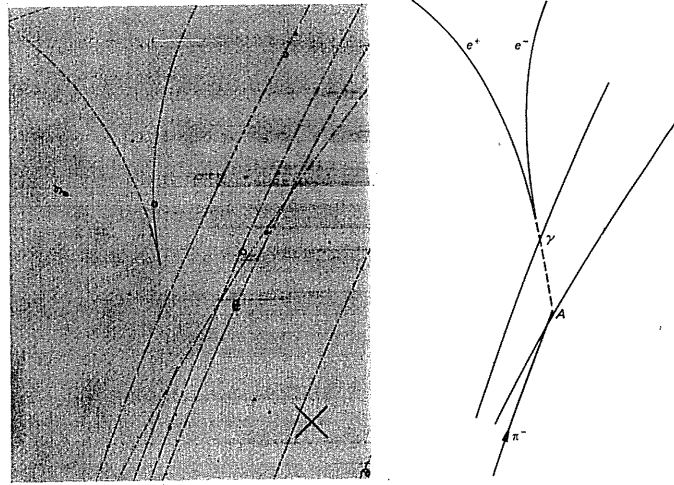
\includegraphics[width=\textwidth]{Imagenes/Camara de niebla.png}
    \captionof{figure}{Desintegración de un fotón en un par electrón-positrón}
    \label{fig: Desint elec-pos}
\end{minipage}
\newpage
\section{Leptones}

\begin{minipage}{0.6\textwidth}
    Como ya hemos mencionado, los leptones son, entre las partículas fundamentales, los fermiones de spin 1/2 que no participan en la interacción fuerte. \\\\
Si nos fijamos, tenemos leptones cargados ($e^-, \mu^-, \tau^-$) y no cargados, los llamados neutrinos. Como los neutrinos no son cargados \textbf{no} pueden participar en los procesos electromagnéticos y sólo participan en procesos \textbf{débiles}, mientras que los leptones cargados participan tanto en procesos electromagnéticos como en débiles.
\end{minipage}
\hfill
\begin{minipage}{0.3\textwidth}
\centering
\begin{tabular}{|c c c|}
\hline
{Nombre}       & {Masa } & {Carga } \\ \hline
$e$                   & 0.511                     & -1                 
\\ 
$\nu_e$    & $<10^{-5}$                & 0                  
\\ \hline
$\mu$                 & 106                       & -1                 
\\ 
$\nu_\mu$             & $<0.2$                    & 0                  
\\ \hline
$\tau$                & 1784                      & -1                 \\ 
$\nu_\tau$            & $<20$                     & 0                  
\\ \hline
\end{tabular}
\captionof{table}{Leptones fundamentales de la materia.}
\label{tab:leptones}
\end{minipage}
\subsubsection{Número leptónico}
A cada una de las familias se les va a asignar un número cuántico conservado, el \textbf{número leptónico}. Cada una de las partículas de una familia tendrán valor +1 mientras que las antipartículas tendrán valor -1.
\begin{tcolorbox}[colback=airforceblue!20, colframe=airforceblue, title=Ejemplo: Conservación del núemero leptónico ]
 Si tenemos la siguiente desintegración$$\gamma \longrightarrow e^-+e^+$$ vemos que el número leptónico al principio de la reacción es nulo, ya que tenemos un fotón mientras que a la derecha, tenemos un +1 que corresponde al electrón y un -1 que corresponde al positrón.\\\\
 La siguiente reacción no podría ser posible
 $$\mu^- \longrightarrow e^- +\gamma$$ ya que no se conservan los números leptónicos, a la izquierda $L_\mu=+1, L_e=0$ y a la derecha $L_\mu=0, L_e=1$, por lo que no se puede dar esta desintegración, la desintegración correcta será $$\mu^- \longrightarrow e^- +\overline{\nu_e}+\nu_\mu$$ Este canal es la manera más probable $\sim 100\%$ que tiene de desintegrarse el muón.
\end{tcolorbox}

El número leptónico se conserva en todos los procesos físico conocidos. Si no exsiten neutrinos en el proceso se reduce a la conservación de pares, por eso los leptones cargados solo pueden crear o destruir pares.
\subsubsection{¿Cómo sabemos que no hay familias de partículas más ligeras que la del electrón?}
Sabemos que no hay más partículas se debe a la estabilidad del electrón, ya que de haberlas, éste tendría que desintegrarse ya que se encontrarían en un estado de energía más bajo.
\newpage
\subsection{Cinemática de partículas cargadas (régimen no relativista)}
Si tenemos una partícula cargada, tiene dos formas de perder energía
\begin{itemize}
    \item \textbf{Colisión elástica}: Una colisión elástica en mecánica cuántica sólo transfiere energía pero no genera nuevos estados. 
    \begin{figure}
        \centering
        \includegraphics[width=0.5\linewidth]{Diagramas Tema 1/ColisionElastica.pdf}
        \caption{Esquema de una colisión elástica. HAY QUE CAMBIARLO}
        \label{fig:Colision Elastica}
    \end{figure}
    De la conservación de la energía y del momento lineal obtenemos
\begin{equation*}
    \begin{aligned}
        &m_1v^2=m_1+u_1^2+m_2u_2^2 \\
        & m_1v_1=m_2u_2 \cos(\phi)+m_1u_1\cos(\theta)\\
        & 0=m_2u_2\sin(\phi)-m_1u_1\sin(\theta)\\
    \end{aligned}
\end{equation*}
Con lo que podemos llegar a la siguiente relación
\begin{equation}
    (m_1+m_2)u_2=2m_1v_1\cos(\phi)
    \label{eq: relacion de transferencia colision elastica}
\end{equation}
Si la energía transferida a la partícula roja, utilizando la relación \ref{eq: relacion de transferencia colision elastica} obtenemos 
\begin{equation}
    \Delta T=\dfrac{1}{2}m_2u_2=\textcolor{red}{\frac{1}{2}} m_2 \frac{4m_1 \textcolor{red}{m_1v_1}}{(m_1+m_2)^2}\cos^2(\phi)= \textcolor{red}{T_\mathrm{i}} \frac{4m_1m_2}{(m_1+m_2)^2} \cos^2(\phi)
\end{equation}
Con lo que podemos obtener el cociente entre la energía transferida respecto a la energía inicial
\begin{equation}
    \frac{\Delta T}{T_\mathrm{i}}=\frac{4m_1m_2}{(m_1+m_2)^2} \cos^2(\phi) 
\end{equation}
Esta transferencia se hace máxima cuando la segunda partícula sale paralela a la trayectoria a la primera, es decir, $\phi=0$. Tenemos dos casos límites
\begin{itemize}
    \item $m_1 \gg m_2$ Para este caso, podemos despreciar $m_2$ en el denominador por lo tanto $\dfrac{\Delta T}{T_\mathrm{i}}=\dfrac{4m_2}{m_1} \xrightarrow[]{}0$, para el caso de un protón y chocando con un electrón $p\xrightarrow[]{}e^-$ la transferencia de energía es del $0.2\%$, esto quiere decir que el protón apenas pierde energía por lo que es muy penetrante.
    \item $m_1\sim m_2$ Para este caso tendremos que la transferencia de energía será \\$\dfrac{\Delta T}{T_\mathrm{i}}=\dfrac{4m_1}{(2m_1)^2} \xrightarrow[]{}1$, para el caso de dos electrones colisionando la transferencia es del $100\%$, por lo que el electrón es muy poco penetrante.
\end{itemize}
     \item \textbf{Radiación de frenado, \textit{Bremsstrahlung}}: Si recordamos cualquier partícula acelerada emite radiación, por lo que cuando una partícula gira, ésta emitirá radiación. Cuando un electrón atraviesa un átomo, recordar que está principalmente vacío, éste interaccionará con el campo electromagnético del átomo \footnote{La contribución principal viene dada por el núcleo}.
     
     \begin{figure}[h]
    \centering
    \includegraphics[]{Diagramas Tema 1/ElectronIntAtomo.pdf}
    \caption{Desviación de una partícula cargada por el campo eléctrico de otra.}
    \label{fig:Desviacion particula}
\end{figure}

     \noindent Si tomamos la expresión no relativista de dicha radiación (fórmula de Larmor)
\begin{equation}
    P=\frac{2}{3}\frac{q^2}{c^3}a^2 \xrightarrow[]{} \qty(\frac{zZ}{m})^2
\end{equation}
Vemos que cuanto mayor masa tenga una partícula menor será la energía emitida por radiación de frenado.

\begin{tcolorbox}[colback=airforceblue!20, colframe=airforceblue, title=Ejemplo: Protón vs electrón]
 Para estudiar las partículas utilizamos aceleradores, si calculamos el cociente entre la masa del protón y la del electrón es $\dfrac{m_p}{m_e}\sim 1900$, el electrón emitirá mucha radiación de frenado mientras que el protón emitirá muy poca, por ello los protones alcanzan energías más altas en los aceleradores de sincrotrón.\\\\
 Como los protones son más penetrantes, son utilizados para tratar tumores de difícil accesibilidad ya que son menos dañinas (aunque más ionizantes), los electrones no traspasan los primeros milímetros de tejido y como transfieren toda su energía provocan mayores daños.
\end{tcolorbox}
Si nos encontramos en el régimen relativista la potencia va como $P\sim m^{-4}$, por lo que se acentúa la diferencia vista en el ejemplo.
\end{itemize}
\subsection{Muones}
Cuando se empezó a estudiar la radiación natural, se pensaba que subiendo en altura detectores disminuiría la radiación ya que se creía que toda provenía del suelo. La sorpresa apareció cuando la radiación no disminuía sino que aumentaba. La radiación que apareció ahora se conocen como \textbf{rayos cósmicos}.
\\\\
Los rayos cósmicos son partículas provenientes del universo que cuando entran en la atmósfera hacen scattering y generan una cascada (\textit{shower}) de partículas hacia la superficie de la Tierra.
\newpage
\begin{figure}
    \centering

    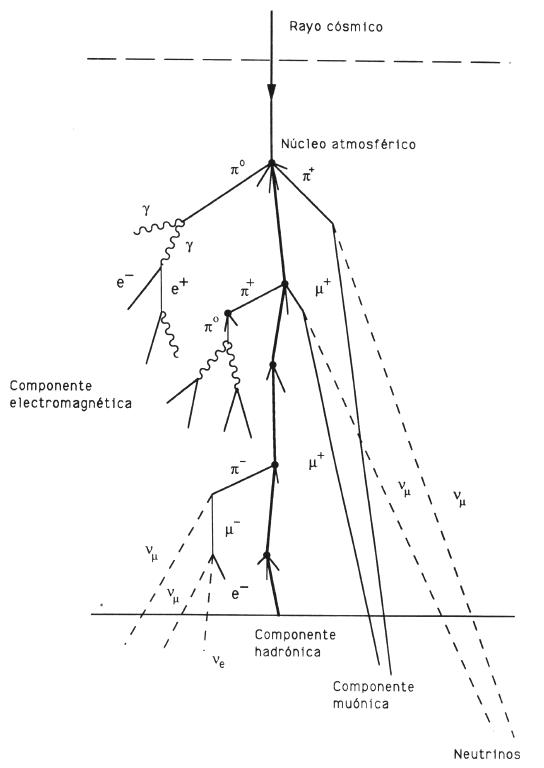
\includegraphics[width=0.85\textwidth]{Imagenes/RayosCosmicos.jpg}
    \caption{Scattering producido por un rayo cósmico. Vemos que se generan cuatro componentes: \textbf{electromagnética}, \textbf{hadrónica}, \textbf{muónica} y \textbf{neutrinos}. La componente electromagnética no atraviesa la atmósfera; de las componentes hadrónicas y muónicas tan sólo nos llegan algunas partículas; los neutrinos atraviesan sin ningún problema tanto la atmósfera como la Tierra.}
    \label{fig: rayo cosmico}
\end{figure}
\clearpage
\subsubsection{Descubrimiento del muón}
    El muón se detectó por primera vez en 1937. Se detectarón a la vez tanto una partícula como una antipartícula. Se teorizó con que se debía a una generación de pares causada por un fotón, aunque el par no era muón-antimuón, sino electrón-positrón pero ambos en un estado excitado.
\subsection{Neutrinos}
Los núcleos atómicos los denotamos como $^A _Z X$, por ejemplo para el plomo 208 tenemos
\begin{itemize}
    \item El número atómico es $Z=82$, que corresponde al número de protones.
    \item  El número de másico es $A=208$, que corresponde a la suma de nucleones dentro del núcleo.
    \item El número de neutrones $N=126$.
\end{itemize}
\begin{figure}[h]
    \centering
    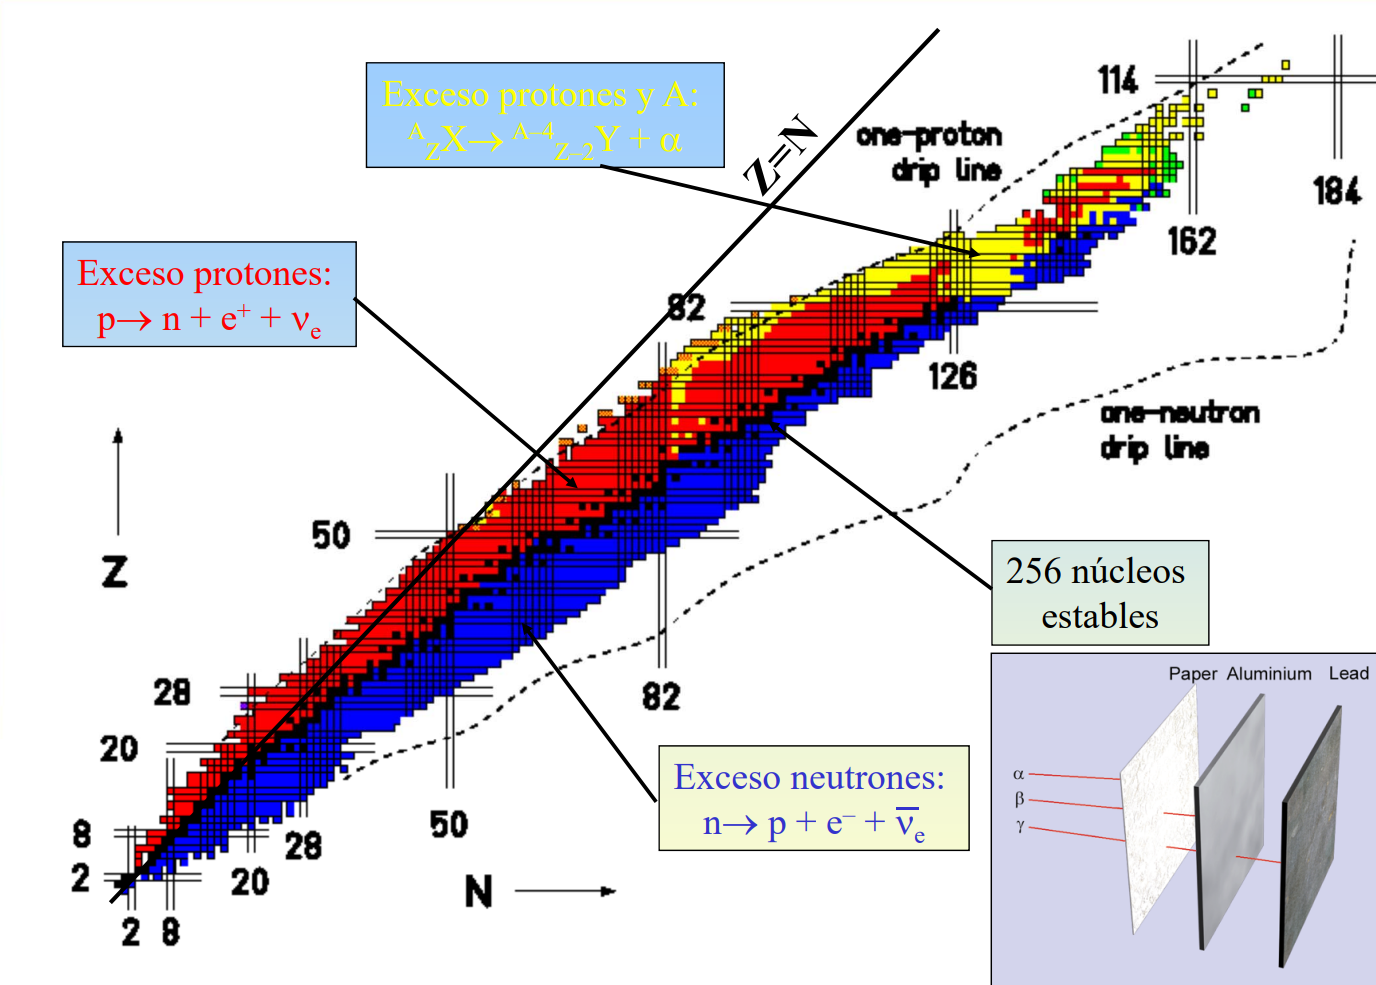
\includegraphics[scale=0.3]{Imagenes/DiagramaSegre.png}
    \captionof{figure}{Diagrama de Segre y capacidad de penetración de los distintos tipos de radiación. La línea negra representa los núcleos con el mismo número de protones y neutrones, la zona azul exceso de neutrones y la zona roja tiene exceso de protones. Las líneas discontinuas se conocen como \textbf{líneas de volteo}, estas líneas encierran la figura por lo que si añadimos por fuera de la inferior un neutrón éste no se ligará, y si añadimos un protón fuera de la superior éste no se ligará.}
    \label{fig: Diagrama Segre}
\end{figure}
Un núcleo puede desintegrarse mediante decaimiento $\beta$. En el diagrama de Segre (figura \ref{fig: Diagrama Segre}), los núcleos de la zona roja se desintegran a partir de decaimiento $\beta^+$, mientras que los que se encuentran en la zona azul tendremos decaimiento $\beta^-$. \footnote{Las partículas entre corchetes es para conservar el número leptónico.}
\newpage
\begin{itemize}
    \item \textbf{Decaimiento $\bm{\beta^-}$}: es la desintegración de un neutrón $n \longrightarrow p+e^-+[x_\nu]$ si tenemos un núcleo $(A,Z) \longrightarrow (A,Z+1)+e^-+[x_\nu]$.
    \item \textbf{Decaimiento $\bm{\beta^+}$}: es la desintegración de un protón $p \longrightarrow n+e^++[y_\nu]$ si tenemos un núcleo $(A,Z) \longrightarrow (A,Z-1)+e^-+[y_\nu]$.
\end{itemize}
Hay otra via para que un protón se transforme en un neutrón, es lo que se conoce como \textbf{captura electrónica}. En un átomo tenemos una posibilidad no nula de encontrar un electrón de la corteza en el núcleo. Cuando esto sucede se da el siguiente proceso $e^-+p\longrightarrow n+[z_\nu]$ y para el núcleo tenemos $e^-+(A,Z) \longrightarrow (A,Z-1)+[z_\nu]$.\\\\
De los decaimiento podemos hacer el estudio a través de las masas de los núcleos
\begin{equation}
    M_1\longrightarrow M_2+m \Rightarrow \Delta M=M_1-M_2-m>0
\end{equation}
En unidades naturales $\Delta M$ es la energía cinética que adquieren tanto $M_2$ como $m$, por lo tanto
\begin{equation*}
    \Delta M=\frac{p^2_{M_2}}{2M_2}+ \frac{p^2_{m}}{2m}
\end{equation*}
Por conservación del momento $\abs{p_{M_2}}=\abs{p_m}$ 
\begin{equation}
    \Delta M=\frac{p^2_{M_2}}{2M_2}+ \frac{p^2_{m}}{2m}=\frac{p^2_{m}}{2m}\qty(1+\frac{m}{M_2})=T_m\qty(1+\frac{m}{M_2})\Rightarrow T_m=\frac{\Delta M}{1+\dfrac{m}{M_2}}
    \label{eq: energia cinetica electron}
\end{equation}
Que para el caso de los decaimientos $\beta^\pm$ de los núcleos todos los valores de las masas son conocidos y son fijos, por lo que $m=m_e\lll M_2$ y  haciendo un desarrollo obtenemos $T_m \simeq \Delta M$, es decir, que la energía cinética del electrón siempre tenía que ser la misma y al ser la partícula más ligera es el que se lleva la mayor parte de la energía cinética.\\

\begin{minipage}{0.6\textwidth}
\begin{tcolorbox}[colback=airforceblue!20, colframe=airforceblue, title=Ejemplo: Desintegración del Bismuto-210]
 Si calculamos la energía que tiene la desintegración del $^{210}\text{Bi}$ en $^{210}\text{Po}$, $M_1=\unit[195600.2]{MeV}, M_2=\unit[195599]{MeV}$, cuya diferencia es de $\unit[1.16]{MeV}$ Por lo que corresponde con el valor que se muestra en la figura \ref{fig: DistribucionElectrones}.\\\\ Al término $\Delta M$ debemos sumarle las aportaciones de las energías de enlace por nucleón y la reionización del átomo para obtener dicha energía.
\end{tcolorbox}
\end{minipage}
\hfill
\begin{minipage}{0.35\textwidth}
    \centering
    \includegraphics[width=\textwidth]{Diagramas Tema 1/DistribucionEnergiaElectrones.pdf}
    \captionof{figure}{Distribución de energía cinética de los electrones}
    \label{fig: DistribucionElectrones}
\end{minipage}\\\\
Pero esto no explicaba que la distribución de energia cinética fuera una suave distribución y no un valor fijo.\\\\
En 1930 Pauli postuló el neutrino, que resolvía el problema de la distribución continua. Y se consiguió detectar en 1956.
\clearpage
\subsubsection{La necesidad del neutrino}
Vamos a analizar la reacción $n \longrightarrow p+e^-$. Si componemos los momentos angulares del protón y del electrón tenemos que componer $\dfrac{1}{2}\otimes \dfrac{1}{2}=0\oplus 1$, es decir, tenemos un bosón. Pero hemos partido de un neutrón, que es un fermión, por lo que si no consideramos que hay una partícula $[x_\nu]$ (como en la ecuacion del decaimiento $\beta^-$ anterior) no se conservaría el momento angular a escala subatómica y eso no puede ser.\\\\
Necesariamente tenemos que introducir una nueva partícula que ha de ser un \textbf{fermión} de spin $\dfrac{1}{2}$. Por lo que si acoplamos los 3 spines $\dfrac{1}{2}$ obtenemos el mismo resultado que la ecuación \ref{eq: Acoplamiento 3 spines 1/2}. Además como en la ecuación anterior sí que se conserva la carga, debe ser \textbf{neutra} y para que no se pueda su masa debía ser \textbf{muy baja} para ya que debía de estar por debajo de la precisión de los instrumentos. \\\\Posteriormente, con la incorporación de los números cuánticos, se determinaría que esta partícula debía ser una antipartícula, como ya denotamos a continuación. \footnote{Estamos introduciendo al neutrino como lo conocemos ahora aunque todavía no hemos determinado si el neutrino tiene antipartícula o no ó si es o no único.}
\subsubsection{Reacciones permitidas y no permitidas}
En toda la sección hemos planteado que el decaimiento $\beta^\pm$ se da en núcleos, pero, ¿se dará si tenemos al protón y al neutrón libres?\\\\
Recordemos que el decaimiento $\beta^-$ es la reacción
\begin{equation}
    n\longrightarrow p+e^-+\overline{\nu_e}
    \label{eq: Decaimiento beta -}
\end{equation}
Mientras que el decaimiento $\beta^+$ es la reacción
\begin{equation}
    p \longrightarrow n+e^++\nu_e
    \label{eq: Decaimiento beta +}
\end{equation}
En la naturaleza no sólo tenemos constricciones en los procesos con los números cuánticos y la carga, sino que también tenemos las ligaduras ``clásicas'': energía, momento lineal, momento angular...\\\\
La reacción \ref{eq: Decaimiento beta -} sí que se puede dar en partículas libres ya que conserva carga, número leptónico y energía, como $m_n-m_p\approx \unit[1.3]{MeV}$, si que nos cabe el electrón. Sin embargo para la reacción \ref{eq: Decaimiento beta +} aunque se conservan la carga y el número leptónico, no se conserva la energía y por eso no está permitida para protones libres.\\\\
Para ``pasar'' en reacciones de un lado a otro de la flecha, necesitamos conjugar la partícula. Por lo tanto de la racción \ref{eq: Decaimiento beta +} obtenemos otra reacción permitida
\begin{equation}
    \overline{\nu_e} + p \longrightarrow n+e^+
    \label{eq: colision proton antineutrino}
\end{equation}
En las colisiones, no tenemos problemas físicos con la energía ya que siempre puede alcanzarse en forma de energía cinética.
\clearpage
\subsubsection{Descubrimiento del neutrino}
En 1930, Hans Bethe propuso una forma de detectar los neutrinos, éstos se habían de detectar de manera indirecta. El procedimiento es el siguiente, mediante una colisión entre un antineutrino y un protón se generan un neutrón y un positrón
\begin{equation}
    \overline{\nu_e} + p \longrightarrow n+e^+
\end{equation}
Ese positrón se aniquila con un electrón dando lugar a un par de fotones, para que se conserve el momento lineal ambos saldrán en direcciones contrarias.
\begin{equation}
    e^++e^-\longrightarrow \gamma + \gamma
    \label{eq: aniquilacion e+ e-}
\end{equation}
Y el neutrón que se genera ha de ser capturado por otro núcleo liberando un fotón, correspondiente a la energía de ligadura.
\begin{equation}
    n+^A_ZX\longrightarrow ^{A+1}_Z X+ \gamma
    \label{eq: captura neutronica}
\end{equation}
En un proceso que se conoce como \textbf{captura neutrónica}.\\\\
Fue así como en 1956 Reines, Clyde y Cowan descubren el neutrino, para ello se fueron a un reactor nuclear, que es un generador de antineutrinos; y colocaron un tanque con agua al lado, después disolvieron en agua una sal de cadmio\footnote{El cadmio tiene una sección de captura neutrónica muy grande.} $(\text{CdCl}_2)$ y observaron primero dos fotones emitidos en direcciones opuestas a la vez y poco después varios fotones
\begin{figure}[h]
\begin{subfigure}[h]{0.45\textwidth}
    \centering
    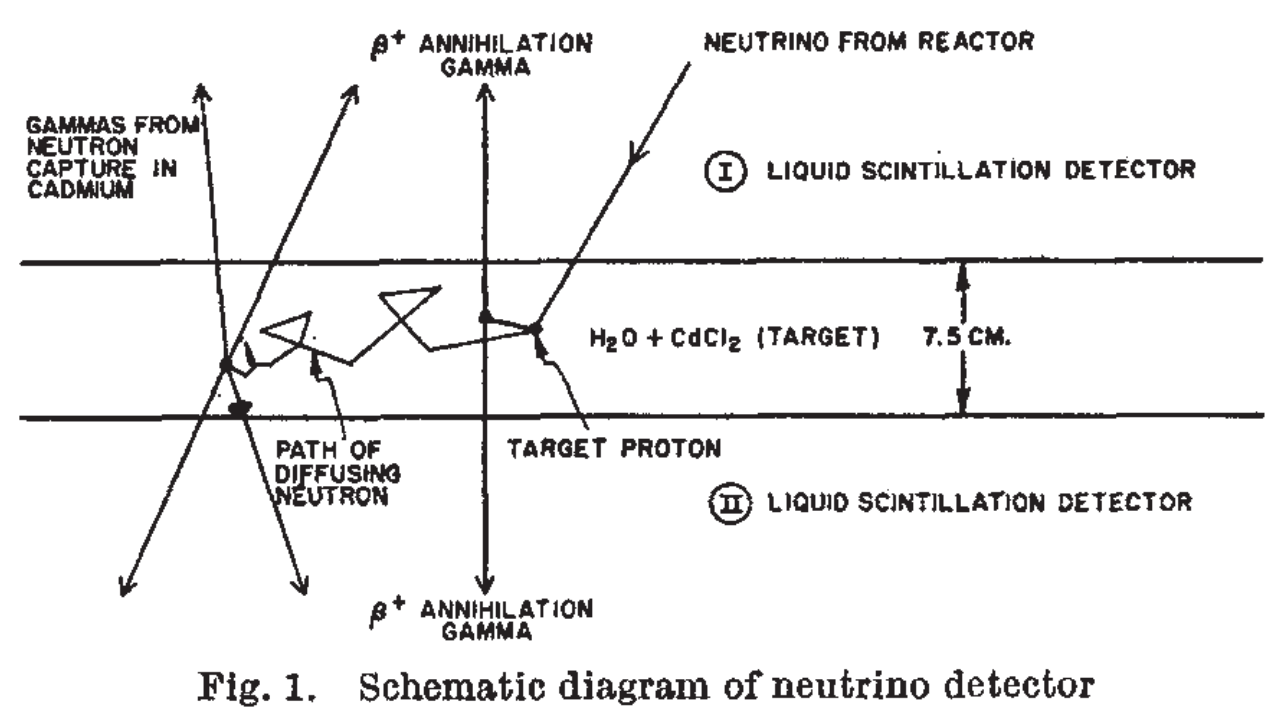
\includegraphics[width=\textwidth]{Imagenes/ExperimentoNeutrino.png}
    \subcaption{Esquema del experimento de detección de neutrinos}
\end{subfigure}
\hfill
\begin{subfigure}[h]{0.45\textwidth}
    \centering
    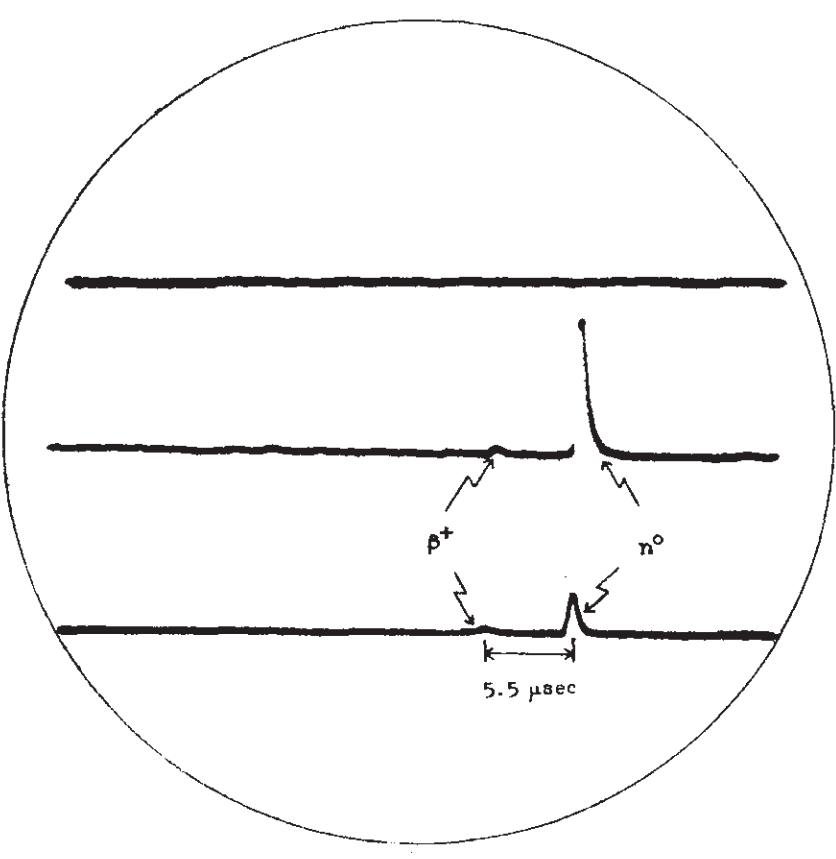
\includegraphics[scale=0.3]{Imagenes/DeteccionNeutrino.png}
    \subcaption{Esquema de la detección del neutrino. \textit{Foto más maravillosa y perfecta de un neutrino.}}
\end{subfigure}
\caption{Diseño del experimento y señal del neutrino. Aunque en la segunda imágen no se aprecia, hay un intervalo entre la primera detección de fotones y la segunda de $\unit[5.5]{\mu s}$, además se detectan dos fotones con diferentes energías al contrario que los detectados por la aniquilación de pares.}
\end{figure}

\noindent Ahora queda estudiar si el neutrino es único, es decir, es sólo perteneciente a una familia, y si tiene no una antipartcula.\\\\
\newpage
\subsubsection{¿Tiene el neutrino antipartícula?}
De los experimentos de Raines y Cowan se obtienen como productos la reacción \ref{eq: colision proton antineutrino}
\begin{equation*}
    \overline{\nu_e} + p \longrightarrow n+e^+ \quad \text{pero no} \quad \nu_e+n\longrightarrow p+e^-
\end{equation*}
Si se diera la segunda reacción tendríamos que los neutrinos interaccionan por de la misma manera con los nucleones del núcleo.
En 1955 se realizó un experimento que se basaba en la siguiente reacción
\begin{equation}
    \nu_e+^{37}_{17}\text{Cl}\longrightarrow e^-+^{37}_{18}\text{Ar}
\end{equation}
Como el Argón tiene un tiempo de vida medio de 35 días, si se producía la reacción debía haber cantidades considerables de Ar.  Si el experimento resultaba positivo el neutrino debía ser igual a su antipartícula y si resultaba negativo no lo eran. Para ello se midieron las reacciones que producían la radiación cósmica y solar sobre un tanque de cloro. Después se enterró el tanque y las reacciones de Ar que se producían eran de la sensibilidad del medidor por lo que se determinó que \textbf{no} eran la misma partícula.
\subsubsection{¿Existen más tipos de neutrinos?}
Así como se determinó que el muón tenía propiedades análogas a las del electrón pero con mayor masa (e inestabilidad), en los años 60 ya había dado tiempo para caracterizar las propiedades del muón (descubierto 30 años antes). \\\\
A finales de los 50 se descubrieron los piones, $\pi^\pm,\pi^0$, los piones tienen un tiempo de desintegración de $\tau\sim \unit[10]{ns}$, los piones decaen en muones a través de
\begin{equation}
    \pi^\pm \longrightarrow \mu^\pm +\nu/\overline{\nu}
    \label{eq: desintegracion piones}
\end{equation}
Para ello se desarrolló un experimento en Brookhaven que consistía en acelerar protones a velocidades ultrarrelativistas.

\begin{figure}[h]
    \centering
    \includegraphics[]{Diagramas Tema 1/ExpBrookhaven.pdf}
    \caption{Esquema del experimento de Brookhaven.}
    \label{fig:ExpBrookhaven}
\end{figure}
Si el neutrino fuera único, es decir, que el producido por desintegración de piones y por decaimiento beta fuera el mismo; en el régimen ultrarrelativista se debían poder dar más o menos la misma proporción de reacciones.
\begin{equation}
\left.
    \begin{aligned}
        & \overline{\nu}+p \longrightarrow n+e^+  \\
    & \nu+n \longrightarrow p+e^-
    \end{aligned}
    \hspace{1cm}
\right\|
\hspace{1cm}
\begin{aligned}
    & \overline{\nu}+p \longrightarrow n+\mu^+ \\
     & \nu+n \longrightarrow p+\mu^-
\end{aligned}
\label{eq: creacion de leptones carados}
\end{equation}
Vamos a explicar la figura \ref{fig:ExpBrookhaven}.  Un haz de protones con una energía cinética de $\unit[15]{GeV}$ choca contra una lámina de berilio generando piones. Estos piones recorren una distancia de $\unit[21]{m}$ hasta llegar al colimador, a lo largo de esta distancia el pion ya se ha desintegrado y hemos obenido muones y neutrinos. Los muones al llegar al detector, compuesto por un bloque de aluminio y un detector de partículas cargadas, han dejado su energía en los primeros $\unit[25]{cm}$ de longitud. Con lo cual los neutrinos debían dar lugar a las reacciones de la ecuación\ref{eq: creacion de leptones carados}, como sólo se detectaban muones, se concluyó que el neutrino no era único sino que había neutrinos de distintas familias.
\\\\
En los apéndices \ref{chap: Apendice A} y \ref{chap: Apendice B} se detalla toda la física necesaria para entender la producción y detección de las partículas más pesadas.
\subsection{La familia Tau}
En 1975 se detectó una pérdida de energía en un scattering de un par electrón-antielectrón,
\begin{equation}
    e^-+e^+\longrightarrow e^\pm +\mu^\mp + \geq \ \text{2 partículas no detectadas}
\end{equation}
Por conservación de carga se determinó que las partículas debían ser cargadas y que se produjeron por pares, como en los electrones y los muones. Cuando se midió la sección eficaz de los eventos se observó un pico como los que encontramos en la figura \ref{fig:Resonancias en seccion eficaz}  %INTRODUCIR LA IMAGEN DE LA SECCIÓN EFICAZ DEL PAPAER DE 1975
Después de un análisis estadístico (bastante pobre pues se hizo estadística con 8 eventos únicamente) se determinó que la masa de las nuevas partículas debía estar entre $\unit[1.6]{GeV/\textit{c}^2}$ y $\unit[2]{GeV/\textit{c}^2}$.
\\\\
Esta hipótesis resultó correcta pues si nos fijamos en la tabla \ref{tab: Particulas elementales} la masa del tau es de $\unit[1784]{GeV/\textit{c}^2}$
\subsubsection{Neutrino Tau}
Como el resto de familias de leptones tenían un neutrino asociado, se sabía que el tau debía tener un neutrino de su misma familia. No fue hasta el año 2001 que se pudo detectar una interacción del nautrino tau. Aunque el experimento realizado era análogo al realizado para la detección de los neutrinos electrónico y muónico, al ser el $\tau$ una partícula tan inestable, no se podía detectar ya que apenas recorría $\unit[2]{mm}$ antes de decaer. Se detectaron 4 eventos: 2 a través del canal
\begin{equation}
    \tau^- \longrightarrow e^-+\nu_\tau+\overline{\nu_e}
\end{equation}
Y otros a través del canal 
\begin{equation}
    \tau^- \longrightarrow h+\nu_\tau+X
\end{equation}
\section{Quarks y hadrones}
Como ya vimos en la sección \ref{subsubsec: Quarks y hadrones} los quarks son fermiones cargados de spin $1/2$ que participan en la interacción fuerte. Como vimos en la tabla \ref{tab: Particulas elementales} se clasifican en 3 familias, los quarks $u$, $c$ y $t$ tienen carga $q=2/3$ mientras que los quarks $d,s$ y $b$ tienen carga $-1/3$, cada uno de ellos tienen a su vez sus propias antipartículas. \\\\ 
Como vemos los quarks no tienen cargas que sean múltiplos enteros de la carga del electrón sino que es fraccionaria, esto hace que en la naturaleza no podamos tener quarks aislados, sino que únicamente podamos tener quarks en agregados de 3 partículas, \textbf{bariones}; o de una partícula y una antipartícula, \textbf{mesones}. De ahí que las masas que aparecene en la tabla \ref{tab: Particulas elementales} sólo se pueda determinar por métodos indirectos.
\subsection{Números cuánticos de los quarks. Sabores}
De manera similar a los leptones, podemos definir números cuánticos para los quarksm, denominados \textbf{sabores}. 
\begin{itemize}
    \item \textbf{Isospín}: Es el sabor asociado a los quarks $u$ y $d$. Asignamos al quark $I(u)=1/2$ y $I(d)=-1/2$ \footnote{En el capítulo 2 veremos que corresponde a la tercera componente de isospín, de momento vamos a quedarnos con el valor absoluto de todo el isospín.}.
    \item \textbf{Extrañeza}: Es el sabor asociado al quark extraño $s$. Se define como $\Tilde{s}=-\qty(N\qty(s)-N\qty(\overline{s}))$.
    \item  \textbf{Encanto}: Es el sabor asociado al quark encantado $c$. Se define como $\Tilde{c}=N\qty(c)-N\qty(\overline{c})$.
    \item \textbf{Belleza}: Es el sabor asociado al quark bottom (bello) $b$. Se define como $\Tilde{b}=-\qty(N\qty(b)-N\qty(\overline{b}))$
\end{itemize}
Todos estos números cuánticos \textbf{se conservan} en procesos \textbf{fuertes} pero \textbf{no se conesrvan} en procesos \textbf{débiles}.
\subsubsection{Número Bariónico}
Todos los quarks tienen un número común, llamado \textbf{número bariónico} $B$. A los quarks se les asigna un número bariónico $B(q)=1/3$ mientras que a los antiquarks se les asigna $B\qty(\overline{q})=-1/3$. Así definimos el número bariónico de un hadrón como \begin{equation}
    B=\frac{1}{3} \qty(N(q)+N\qty(\overline{q}))
\end{equation}
Obteniendo así que los bariones tienen número bariónico 1 y los mesones 0. Este número cuántico \textbf{se conserva} en todos los procesos físicos conocidos. 

\subsection{El zoo de las partículas elementales}
\noindent
\begin{minipage}{0.45\textwidth}
    En las tablas \ref{tab: Bariones} y \ref{tab: Mesones} se recogen las principales características de los mesones y los bariones.\\\\
    Como vemos en la figura \ref{fig: Zoo particulas} tenemos una cantidad ingente de partículas hacia el año 1955. W.Lamb en ese mismo año durante su discurso del nóbel dijo: \textit{Maybe physicists discovering a new particle ought to be fine 10.000}
\end{minipage}
\hfill
\begin{minipage}{0.45\textwidth}
    \centering
    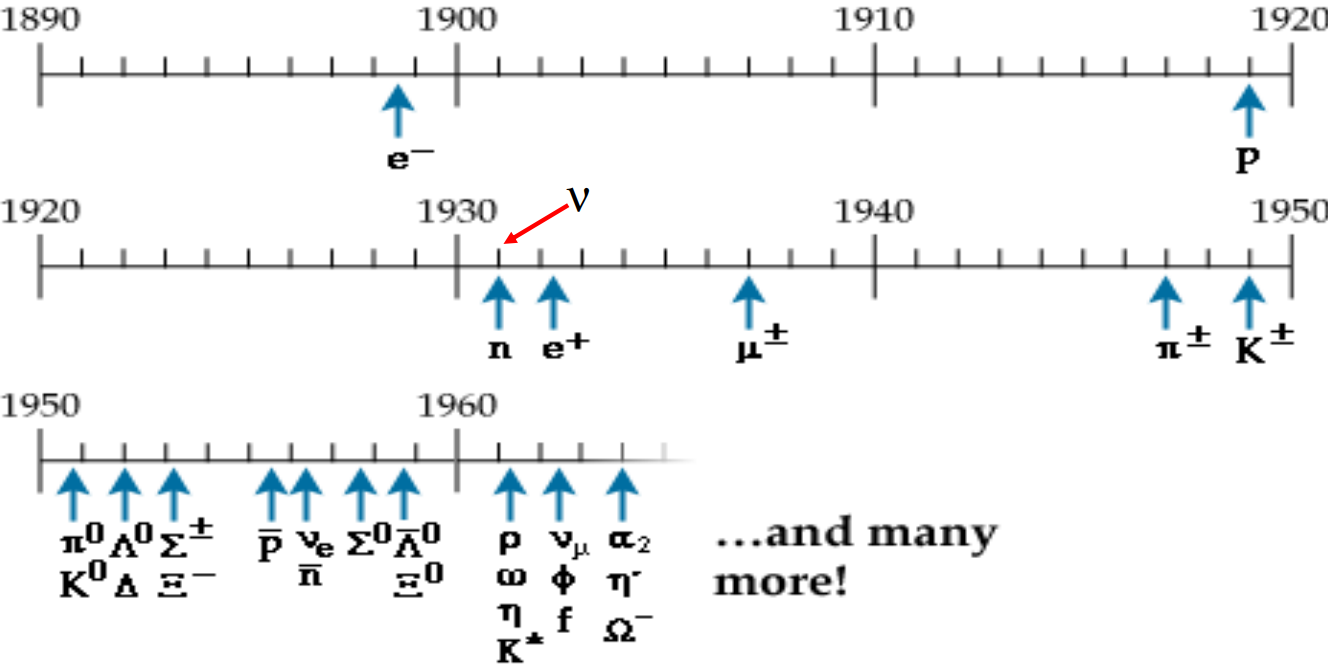
\includegraphics[width=\linewidth]{Imagenes/ParticleZoo.png}
    \captionof{figure}{Línea temporal del descubrimiento de las partículas elementales.}
    \label{fig: Zoo particulas}
\end{minipage}
\begin{table}[h]
    \centering
\begin{tabular}{|c|c|c|c|c|c|c|c|}
\hline
Barión            & $Q$  & Quarks       & $I$    & $\Tilde{s}$ & $\Tilde{c}$ & $\Tilde{b}$ & Masa   \\ \hline
$p^{+}$           & $+1$ & \textit{uud} & $1/2$  & 0           & 0           & 0           & 938.3  \\
$n^{0}$           & $0$  & \textit{udd} & $1/2$  & 0           & 0           & 0           & 939.6  \\
$\Delta^{++}$     & $+2$ & \textit{uuu} & $3/2$  & 0           & 0           & 0           & 1232   \\
$\Delta^{+}$      & $+1$ & \textit{uud} & $3/2$  & 0           & 0           & 0           & 1232   \\
$\Delta^{0}$      & $0$  & \textit{udd} & $3/2$  & 0           & 0           & 0           & 1232   \\  \hline \hline
$\Lambda^{0}$     & $0$  & \textit{uds} & $0$    & -1          & 0           & 0           & 1115.7 \\
$\Sigma^{0}$      & $0$  & \textit{uds} & $1$    & -1          & 0           & 0           & 1192.6 \\
$\Sigma^{+}$      & $+1$ & \textit{uus} & $1$    & -1          & 0           & 0           & 1189.4 \\
$\Sigma^{-}$      & $-1$ & \textit{dds} & $1$    & -1          & 0           & 0           & 1197.4 \\
$\Xi^{0}$         & $0$  & \textit{uss} & $1/2$  & -2          & 0           & 0           & 1314.8 \\
$\Xi^{-}$         & $-1$ & \textit{dss} & $1/2$  & -2          & 0           & 0           & 1321.7 \\
$\Omega^{-}$      & $-1$ & \textit{sss} & $0$    & -3          & 0           & 0           & 1672.5 \\ \hline \hline
$\Lambda_{c}^{+}$ & $+1$ & \textit{udc} & $0$    & 0           & 1           & 0           & 2286.5 \\
$\Sigma_{c}^{0}$  & $0$  & \textit{udc} & $1$    & 0           & 1           & 0           & 2453.8 \\
$\Sigma_{c}^{+}$  & $+1$ & \textit{uuc} & $1$    & 0           & 1           & 0           & 2452.9 \\
$\Sigma_{c}^{++}$ & $+2$ & \textit{uuc} & $1$    & 0           & 1           & 0           & 2453.8 \\
$\Xi_{c}^{0}$     & $0$  & \textit{usc} & $1/2$  & -1          & 1           & 0           & 2470.9 \\
$\Xi_{c}^{+}$     & $+1$ & \textit{dsc} & $1/2$  & -1          & 1           & 0           & 2467.8 \\
$\Omega_{c}^{0}$  & $0$  & \textit{ssc} & $0$    & -2          & 1           & 0           & 2695.2 \\
$\Xi_{c}^{++}$ & $+2$ & \textit{ccu} & $1/2$  & -1          & 2           & 0           & 2766.0 \\
$\Omega_{cc}$  & $+1$ & \textit{ccs} & $1/2$  & -1          & 2           & 0           & 2766.0 \\ \hline \hline
$\Lambda_{b}^{0}$ & $0$  & \textit{udb} & $0$    & 0           & 0           & -1          & 5619.6 \\
$\Sigma_{b}^{-}$  & $-1$ & \textit{ddb} & $1$    & 0           & 0           & -1          & 5815.5 \\
$\Sigma_{b}^{0}$  & $0$  & \textit{udb} & $1$    & 0           & 0           & -1          & 5812.7 \\
$\Sigma_{b}^{+}$  & $+1$ & \textit{uub} & $1$    & 0           & 0           & -1          & 5807.8 \\
$\Xi_{b}^{-}$     & $-1$ & \textit{usb} & $1/2$  & -1          & 0           & -1          & 5791.9 \\
$\Xi_{b}^{0}$     & $0$  & \textit{dsb} & $1/2$  & -1          & 0           & -1          & 5793.1 \\
$\Omega_{b}^{-}$  & $-1$ & \textit{ssb} & $0$    & -2          & 0           & -1          & 6046.1 \\
$\Omega_{b}^{++}$ & $+2$ & \textit{bbq} & $1/2$  & 0           & 0           & -2          & 6100.0 \\
$\Omega_{bb}^{+}$  & $+1$ & \textit{bbq} & $1/2$  & 0           & 0           & -2          & 6100.0 \\
$\Omega_{bbb}^{-}$  & $-1$ & \textit{bbb} & $0$    & 0           & 0           & -3          & 6100.0 \\ \hline
\end{tabular}
\caption{Bariones y sus principales propiedades. La tabla \ref{tab: Bariones} está dividida en 4 cuadrados, cada uno de ellos tiene asociado un sabor, isospín, extrañeza, encanto y belleza, respectivamente.}
\label{tab: Bariones}
\end{table}

\newpage
\begin{table}[h]
    \centering
    \begin{tabular}{|c|c|c|c|c|c|c|c|c|} \hline 
        Mesón & $Q$ & Quarks & $J$ &  \textit{I} & $\tilde{s}$ & $\tilde{c}$ & $\tilde{b}$ & Masa \\ 
        \hline 
        $\pi^{0}$ & $0$ & $u\bar{u} - d\bar{d}$ & 0 & 1 & 0 & 0 & 0 & 134.98 \\ 
        $\pi^{+}$ & $+1$ & $u\bar{d}$ & 0 & 1 & 0 & 0 & 0 & 139.57 \\ 
        $\pi^{-}$ & $-1$ & $d\bar{u}$ & 0 & 1 & 0 & 0 & 0 & 139.57 \\ 
        $\rho^{0}$ & $0$ & $u\bar{u} - d\bar{d}$ & 1 & 1 & 0 & 0 & 0 & 775.26 \\ 
        $\rho^{+}$ & $+1$ & $u\bar{d}$ & 1 & 1 & 0 & 0 & 0 & 775.26 \\ 
        $\rho^{-}$ & $-1$ & $d\bar{u}$ & 1 & 1 & 0 & 0 &0 & 775.26 \\ 
        \hline \hline 
        $K^{0}$ & $0$ & $d\bar{s}$ & 0 & 1/2 & -1 & 0 & 0 & 497.61 \\ 
        $K^{+}$ & $+1$ & $u\bar{s}$ & 0 & 1/2 & -1 & 0 & 0 & 493.68 \\ 
        $K^{*-}$ & $-1$ & $s\bar{u}$ & 1 & 1/2 & -1 & 0 & 0 & 891.66 \\ 
        $K^{*0}$ & $0$ & $s\bar{d}$ & 1 & 1/2 & -1 & 0 & 0 & 896.10 \\ 
        $\phi^{0}$ & $0$ & $s\bar{s}$ & 1 & 0 & -2 & 0 & 0 & 1019.46 \\ 
        $\omega^{0}$ & $0$ & $u\bar{u} + d\bar{d}$ & 1 & 0 & 0 & 0 & 0 & 782.65 \\ 
        $\eta^{0}$ & $0$ & $u\bar{u} + d\bar{d} - 2s\bar{s}$ & 0 & 0 & -2 & 0 & 0 & 547.86 \\ 
        $\eta'^{0}$ & $0$ & $u\bar{u} + d\bar{d} + s\bar{s}$ & 0 & 0 & -1 & 0 & 0 & 957.78 \\ 
        \hline \hline 
        $J/\psi^{0}$ & $0$ & $c\bar{c}$ & 1 & 0 & 0 & +1 & 0 & 3096.9 \\ 
        $\eta_{c}^{0}$ & $0$ & $c\bar{c}$ & 0 & 0 & 0 & +1 & 0 & 2983.9 \\ 
        $D^{+}$ & $+1$ & $c\bar{d}$ & 0 & 1/2 & 0 & +1 & 0 & 1869.6 \\ 
        $D^{0}$ & $0$ & $c\bar{u}$ & 0 & 1/2 & 0 & +1 & 0 & 1864.8 \\ 
        $D^{*+}$ & $+1$ & $c\bar{d}$ & 1 & 1/2 & 0 & +1 & 0 & 2010.3 \\ 
        $D^{*0}$ & $0$ & $c\bar{u}$ & 1 & 1/2 & 0 & +1 & 0 & 2006.9 \\ 
        $D_{s}^{+}$ & $+1$ & $c\bar{s}$ & 0 & 0 & -1 & +1 & 0 & 1968.3 \\ 
        $D_{s}^{*+}$ & $+1$ & $c\bar{s}$ & 1 & 0 & -1 & +1 & 0 & 2112.2 \\ 
        \hline \hline 
        $\Upsilon^{0}$ & $0$ & $b\overline{b}$ & 1 & 0 & 0 & 0 & 0 & 9460.3 \\ 
        $\eta_{b}^{0}$ & $0$ & $b\bar{b}$ & 0 & 0 & 0 & 0 & 0 & 9399.0 \\ 
        $B^{+}$ & $+1$ & $u\bar{b}$ & 0 & 1/2 & 0 & 0 & +1 & 5279.3 \\ 
        $B^{0}$ & $0$ & $d\bar{b}$ & 0 & 1/2 & 0 & 0 & +1 & 5279.6 \\ 
        $B^{*+}$ & $+1$ & $u\bar{b}$ & 1 & 1/2 & 0 & 0 & +1 & 5325.1 \\ 
        $B^{*0}$ & $0$ & $d\bar{b}$ & 1 & 1/2 & 0 & 0 & +1 & 5325.2 \\ 
        $B_{s}^{0}$ & $0$ & $s\bar{b}$ & 0 & 0 & -1 & 0 & +1 & 5366.8 \\ 
        $B_{s}^{*0}$ & $0$ & $s\bar{b}$ & 1 & 0 & -1 & 0 & +1 & 5415.4 \\ 
        $B_{c}^{+}$ & $+1$ & $c\bar{b}$ & 0 & 0 & 0 & +1 & +1 & 6274.9 \\ 
        $B_{c}^{*+}$ & $+1$ & $c\bar{b}$ & 1 & 0 & 0 & +1 & +1 & 6332.5 \\ 
        \hline 
    \end{tabular}
    \caption{Mesones y sus propiedades (la $J$ es el spin). En la tabla \ref{tab: Mesones} todas las combinaciones lineales están normalizadas. }
    \label{tab: Mesones}
\end{table}

\clearpage
\subsection{Hipótesis de los tres quarks ligeros} \label{subsec: hipotesis tres quarks ligeros}
En el año 1964, Murray Gell-Mann, a través de la teoría de grupos desarrolló una teoría para explicar la constitución de los bariones y los mesones. Postuló que las partículas fundamentales estaban constituidas por un \textbf{triplete unitario}, constituido por 
\begin{itemize}
    \item \textbf{Singlete isotópico} $(s)$: tenía carga $z$ en unidades de $e$.
    \item \textbf{Doblete isotópico} $(u,d)$ con carga $z+1$ y $z$ respectivamente.
\end{itemize}
Que fuesen tres partículas requería que estas partículas fundamentales fueran fermiones de spin 1/2 y tuvieran carga fraccionaria en unidades de $e$, $z=-1/3$. A estas partículas las denominó quarks.
\subsubsection{Representacion en la teoría de grupos}
La teoría de grupos nos permite tener representaciones irreducibles de los diagramas de Gell-Mann, cada una de estas representaciones corresponde a un grupo de partículas según el acoplamiento de los quarks.
\begin{figure}[h]
    \centering
    % Primera subfigura
    \begin{subfigure}[h]{0.3\textwidth}
        \centering
        \includegraphics[scale=0.65]{Diagramas Tema 2/DGellmanJP=0-.pdf}
    \end{subfigure}
   \hfill
    % Segunda subfigura
    \begin{subfigure}[h]{0.3\textwidth}
        \centering
        \includegraphics[scale=0.65]{Diagramas Tema 2/DGellManJP=1_2+.pdf}
    \end{subfigure}
    \hfill % Espacio entre subfiguras
    % Tercera subfigura
    \begin{subfigure}[h]{0.3\textwidth}
        \centering
        \includegraphics[scale=0.65]{Diagramas Tema 2/DGellManJP=3_2+.pdf}
    \end{subfigure}
    \caption{Diferentes diagramas de Gell-Mann.}
    \label{fig:figura_general}    
\end{figure}
\subsection{Descubrimiento de los quarks}
En 1954 Chambers y Hofstader realizaron un experimento donde demostraban que el protón tenía estructura a través de un scattering elástico de electrones de alta energía. El resultado que obtuvieron fue que el protón tenía un radio cuadrático medio distinto de 0, lo cual implicaba que no era puntual. En el apéncice \ref{chap: Apendice C} se desarrolla la teoría necesaria para entender cómo funciona el experimento.
\\\\
Más tarde en 1967, Friedmann, Kendall y Taylor en SLAC, demostraron la dispersión violenta del electrón producida por tres partículas puntuales, los quarks.
\subsubsection{Descubrimiento del quark encantado}
El 2 de diciembre de 1974 se publicaron en \textit{Physical Review Letters} dos artículos seguidos de dos experimentos uno en SLAC y otro en Brookhaven, sobre la observación de una resonancia muy estrecha en colisiones electrón-positrón (a la 
partícula se le denominó $\psi$) y la observación de una nueva partícula pesada, respectivamente (a la partícula se le denominó $J$). \\\\
La resonancia tenía una energía $E=\unit[3.1]{GeV}$ y una anchura de desintegración $\Gamma=\unit[1.3]{MeV}$ si nos fijamos en la regla de oro de Fermi \ref{eq: regla de oro de fermi}, como la densidad de estados es muy grande, el término correspondiente al elemento de matriz del potencial tenía que ser muy pequeño, es decir era un evento muy poco probable.
\subsubsection{Descubrimiento del bottom y top}
En 1977 en FermiLab se deterctaron tres resonancias del mesón $\Upsilon$ a través de una colisión protón-núcleo con una energía en el centro de masas de $\unit[400]{GeV}$.\\\\
En 1995 se consiguió medir en Fermilab, a través de colisiones de $\sqrt{s}=\unit[1.8]{TeV}$, el decaimiento de un par top-antitop en dos W y un par bottom. Este último descubrimiento es uno de las predicciones más robustas del modelos standard.
\pagestyle{fancy}
\fancyhead[R]{Física Nuclear y de Partículas: Tema 2}
\fancyhead[L]{4º Grado en Física}
\chapter{Interacciones fundamentales. Leyes de conservación}
\section{Partículas virtuales}
\noindent
\begin{minipage}{0.6\textwidth}
    De manera clásica, cuando introducimos una partícula con carga\footnotemark en el vacío, ésta genera un campo (líneas de campo). Si introducimos otra partícula que tiene el mismo tipo de carga, ésta se verá influida por el campo que ha generado la primera partícula.\\\\
    En mecánica cuántica las interacciones no están mediadas por los campos ``clásicos'' generados por las partículas, sino por partículas denominadas \textbf{bosones gauge} intercambiando momento.
\end{minipage}
\footnotetext{Entendemos carga como la carga asociada a la fuerza.}
\hfill
\begin{minipage}{0.35\textwidth}
    \centering
    \includegraphics[scale=1.2]{Diagramas Tema 2/ParticulaClasica.pdf}
    \captionof{figure}{Campo generado por una partícula clásica.}
    \label{fig: campoclasico}
\end{minipage}\\\\
\noindent \begin{minipage}{0.6\textwidth}
    Si consideramos un electrón siendo influido por una distribución de carga, el bosón gauge del campo electromagnético es el \textbf{fotón}. Vamos a estudiar el scattering desde el sistema CM, para ello nos vamos al vértice del diagrama:
    \begin{itemize}
        \item \textbf{Conservación del momento}:En el vértice pasamos de $e^-(m_ec^2,\vec{0}) \longrightarrow e^-(E_k,-\vec{k}) +
 \gamma(kc,\vec{k})$
        \item \textbf{Conservación de la energía}: En el vértice se conserva la energía $mc^2=\sqrt{m^2c^4+k^2c^2}+kc$, como $\abs{k}\ge 0$ la energía sólo se conserva si $\abs{k}=0$ por lo que, ¿no existe el fotón?
    \end{itemize}
\end{minipage}
\hfill
\begin{minipage}{0.35\textwidth}
    \centering
    \includegraphics[]{Diagramas Tema 2/ElectronDistribcarga.pdf}
    \captionof{figure}{Scattering de un electrón por una distribución de carga.}
    \label{fig: scattering electron y distribucion de carga}
\end{minipage}\\\\
Vamos a hacer de nuevo el análisis pero con partículas masivas. Si tenemos una interacción entre dos partículas $A$ y $B$ de masas $M_A$ y $M_B$ respectivamente que intercambian una partícula masiva $X$ con masa $M_X$ y volvemos realizar el mismo estudio:
\clearpage
\begin{figure}
    \centering
    \includegraphics[width=0.5\linewidth]{Diagramas Tema 2/IntAyB.pdf}
    \caption{Interacción de dos partículas a través de una partícula masiva.}
    \label{fig: intayb}
\end{figure}
\noindent En el primer vértice (línea A) tenemos
    \begin{equation*}
        \begin{aligned}
            &A(M_Ac^2,\vec{0})\longrightarrow A(M_Ac^2,\vec{p})+X(M_Xc^2,-\vec{p})\\ &\Delta E=E_A+E_X-M_Ac^2=\sqrt{M_A^2c^4+p^2c^2}+\sqrt{M_X^2c^4+p^2c^2}-M_Ac^2
        \end{aligned}
    \end{equation*}
Pero antes dijimos que para que se cumpla la conservación de energía la contribución de la energía debía ser nula, por lo que tenemos una \textbf{violación de la conservación energía en el vértice}.\\\\
Esta violación de la conservación de energía \textbf{está permitida} por el principio de incertidumbre, si recordamos
\begin{equation*}
    \Delta E\, \Delta t\sim \hbar \quad  \text{como} \quad E=\sqrt{M^2c^4+p^2c^2}  \Rightarrow \Delta t\sim \frac{\hbar}{\Delta E}
\end{equation*}
Por lo que cuanto mayor sea el incremento de energía, menos tiempo se podrá violar la conservación de energía. Por lo que nos encontramos con dos casos límite
\begin{equation*}
    \Delta E =\left\{\begin{aligned}
    & p \gg M_i \longrightarrow \sqrt{p^2c^2}+\sqrt{p^2c^2}-\cancel{M_Ac^2}=2pc\\
    & p \ll M_i \longrightarrow\sqrt{M_A^2c^4}+\sqrt{M_X^2c^4}-M_Ac^2= M_Xc^2
    \end{aligned} \right.
\end{equation*}
Es concretamente este tipo de partícula lo que conocemos como \textbf{partícula virtual}, es una partícula que no se puede medir ya que su tiempo de vida es tan corto que no podemos medir sus propiedades físicas.\\\\
Entonces como para cualquier valor del momento $\Delta E\ge M_X c^2$  se podrá violar la conservación de energía un tiempo $\tau\sim \dfrac{\hbar}{M_Xc^2}$, ésto nos permite definir una distancia de viaje máxima de las partículas virtuales a través de la expresión $R=c\tau$, que para el caso del fotón como $M_\gamma=0 \Rightarrow \tau= \infty$  y por lo tanto el alcance de dicha interacción es infinito, como ya sabíamos.\\\\
Para el caso de las partículas sin masa como los fotones virtuales \textbf{tampoco se pueden medir} ya que no cumplen la ecuación $E=pc$ ya que se les puede asociar una masa efectiva además de otras características que no tienen los fotones reales.\clearpage
Para otras interacciones tendremos 
\begin{itemize}
    \item \textbf{Interacción débil}: $M_{W^\pm,Z^0}\equiv \unit[80-90]{GeV} \longrightarrow R_\text{Débil}=\unit[2\cdot 10^{-3}]{fm}$, es decir, tienen que estar prácticamente pegadas.
    \item \textbf{Interacción nuclear fuerte}: El alcance que tiene es de $R_\text{fuerte}=\unit[1-2]{fm}$, por lo que la masa de la partícula mediadora debe tener una masa $M\equiv \unit[100-200]{MeV}$. Ésta fue la predicción de Yukawa y en 1947 se descubrió el $\pi^0$ con una masa $M=\equiv \unit[140]{MeV}$.
\end{itemize}
La razón por la que se especifica interacción \textit{nuclear} fuerte, se debe a que es una fuerza residual \footnote{Los quarks tienen color pero sus estados ligados como el protón y el neutrón han de tener color nulo. Sin embargo, cuando están muy cerca los quarks de diferentes nucleones pueden ``verse'' y de ahí nace la fuerza nuclear fuerte.} generada por la interacción fuerte (al igual que las fuerzas de Van der Waals nacen de la interacción electromagnética). La interacción fuerte está mediada por gluones, que son partículas sin masa pero no tiene alcance infinito como la electromagnética, volveremos a este problema más adelante. \label{sec: particulas virtuales}
\section{Intensidad entre interacciones}
\subsection{Potencial de Yukawa}
Si partimos de la ecuación de Klein-Gordon \ref{eq: Ecuacion de Klein-Gordon} para una patícula con masa
\begin{equation}
    -\frac{\hbar^2}{c^2} \pdv[2]{\phi(\vec{r},t)}{t}=-\hbar^2\grad^2\phi(\vec{r},t)+m^2c^2\phi(\vec{r},t)
\end{equation}
obtenemos la ecuación de propagación de un campo bosónico (masivo) arbitrario. Si nuestra función de onda no es función del tiempo, la ecuación resulta la Ecuación de Poisson
\begin{equation}
    \grad^2\phi(\vec{r})=\frac{m^2c^2}{\hbar^2} \phi(\vec{r}) \xrightarrow[\text{Espacio isótropo}]{R=\hbar/mc} \phi(\vec{r})=\phi(r) \Rightarrow \frac{1}{r^2} \pdv{}{r}\qty(r^2\pdv{\phi(r)}{r})=\frac{\phi(r)}{R^2}
\end{equation}
Donde hemos utilizado el laplaciano en esféricas y sólo tenemos contribución de la parte radial por ser el espacio isótropo. Por encontrarnos en esféricas $r>0$ y la solución que encontramos a esta ecuación es 
\begin{equation}
    \phi(r)=\frac{g}{4\pi\,r} \exp{-\dfrac{r}{R}}
    \label{eq: potencial de yukawa}
\end{equation}
Donde $g$ es una constante que nos dará la carga del campo asociado. Para el campo EM la ecuación resultaría la ecuación de Laplace y recuperamos el potencial coulombiano. En el sistema de unidades de Lorentz-Heaviside $(\mu_0=\epsilon_0=1)$
\begin{equation}
    \phi(r)=\frac{g}{4\pi} \frac{1}{e} \Rightarrow V(r)=e \phi(r)=\textcolor{red}{\frac{e^2}{4\pi}}\frac{1}{r} \frac{\hbar c}{\textcolor{red}{\hbar c}}=\textcolor{red}{\alpha} \frac{\hbar c}{r}.
\end{equation}
\clearpage

\subsubsection{Propagadador del potencial de Yukawa}
Si recuperamos el desarrollo que hicimos en el apéndice \ref{chap: Apendice C} la ecuación \ref{eq: transformada de fourier potencial de yukawa} 
$$I_2=\dfrac{4\pi}{\qty(\dfrac{q}{\hbar})^2+\qty(\dfrac{1}{R})^2}$$
es la transformadad de Fourier del potencial de Yukawa salvo la constante de normalización, por lo tanto
\begin{equation}
    A(q)=\frac{g}{4\pi} \dfrac{4\pi}{\qty(\dfrac{q}{\hbar})^2+\qty(\dfrac{1}{R})^2}=g \,\dfrac{\qty(\hbar c)^2}{q^2c^2+M^2c^4}
\end{equation}
Donde hemos vuelto a utilizar que $R=\dfrac{\hbar}{mc}$. Si a la transformada del potencial la multiplicamos por $g$ obtendremos el \textbf{progador}, es equivalente al potencial pero en el espacio de momentos.
\begin{equation}
    f(q)=gA(q)=g^2 \,\dfrac{\qty(\hbar c)^2}{q^2c^2+M^2c^4}
\end{equation}
Podemos definir entonces las constantes de la interacción $g$ como $\alpha_g=\dfrac{g^2}{4\pi \hbar c}$ y el propagador tendrá la forma
\begin{equation}
     f(q)=4\pi \alpha_g\,\dfrac{\qty(\hbar c)^3}{q^2c^2+M^2c^4}
     \label{eq: propagador de yukawa}
\end{equation}
Esta constante $\alpha_g$ nos permitirá saber la intensidad que tiene cualquier interacción. \\\\
A través de la regla de oro de Fermi $\lambda=\dfrac{2\pi}{\hbar} \rho(E) \abs{\mel{f}{V}{i}}^2 \ \text{con} \ \rho(E)=f(\Delta E)$, podemos calcular la  probabilidad de interacción. Como $\lambda\sim \abs{f(q)}^2\sim \alpha_g^2$, la constante de la interacción nos indicará cual es el \textbf{canal más probable para una interacción} (siempre que esté permitido).
\subsubsection{Amplitud de scattering y vértices en los diagramas de Feymann}
Cuando se da una interacción entre partículas, cada una de las partículas tiene un tipo de carga $g$, por lo tanto cuando representamos la interacción en un diagrama de Feymann, cada vértice contribuirá con una cantidad de carga $Z\cdot g$, esto quiere decir que el vértice en el diagrama de Feymann tendrá un valor de $Z\sqrt{\alpha_g}$ ya que recordemos que $\alpha_g\sim g^2$.\\\\
La amplitud de scattering es el elemento de matriz de la regla de oro de Fermi, este elemento va como el producto de cada uno de los vértices del diagrama. Por otro lado la sección eficaz va como el cuadrado del elemento.

\begin{tcolorbox}[colback=airforceblue!20, colframe=airforceblue, title=Ejemplo: Interacción electromagnética]
 En la figura \ref{fig: Interacciones electrones} se represetan dos interacciones permitidas entre electrones, como son de tipo electromagético, la constante de la interacción es la de estructura fina. Las amplitudes y secciones de cada uno de los procesos van como
 \begin{itemize}
     \item Proceso \ref{fig: interaccion electrones sin loop}: \textbf{Amplitud}: $\alpha$ \textbf{Sección eficaz}: $\alpha^2$
     \item Proceso \ref{fig:interaccion loop} \textbf{Amplitud} $\alpha^2$ \textbf{Sección Eficaz}: $\alpha^4$
 \end{itemize}
 Y como la probabilidad de que se de un proceso es proporcional a la sección eficaz, para el caso de la interacción electromagnética $\alpha \sim 10^{-2}$ estos procesos se pueden despreciar frente a otros a la hora de desarrollar una teoría. Pasa lo mismo con las correcciones de estructura fina del átomo de hidrógeno, como las contribuciones a la energía van con $\alpha^2$ se pueden despreciar o tratarse de manera \textbf{perturbativa}
\end{tcolorbox}
\begin{figure}[h!]
    \centering
    % Subfigura 1
    \begin{subfigure}{0.45\textwidth}
        \centering
        \includegraphics[width=0.65\textwidth]{Diagramas Tema 2/IntElectrones.pdf}
        \caption{Interacción electrón-electrón a través de un fotón}
        \label{fig: interaccion electrones sin loop}
    \end{subfigure}
    \hfill
    % Subfigura 2
    \begin{subfigure}{0.45\textwidth}
        \centering
        \includegraphics[width=\textwidth]{Diagramas Tema 2/IntElectronesLoop.pdf}
        \caption{Interacción electrón-electrón a través de un fotón que crea un par electrón-positrón.}
        \label{fig:interaccion loop}
    \end{subfigure}
    
    \caption{Diagramas de Feymann de dos interacciones posibles entre electrones}
    \label{fig: Interacciones electrones}
\end{figure}
\subsection{Constantes de interacciones. Intensidad de las interacciones}
Vamos a calcular las constantes de las interacciones que explicamos al principio del capítulo. Para las dos primeras vamos a considerar un sistema de dos protones separados una distancia $R$\\\\
\noindent
\begin{minipage}{0.4\textwidth}
    \subsubsection{Interacción electromagnética}
El potencial electromagnético se puede escribir como
\begin{equation*}
    V(r)=\frac{e^2}{4\pi \varepsilon_0 } \frac{1}{R} \frac{\hbar c}{\hbar c}= \alpha \frac{\hbar c}{R}
\end{equation*}
El valor de $\alpha\sim 10^{-2}$
\end{minipage}
\hfill
\begin{minipage}{0.5\textwidth}
    \subsubsection{Interacción gravitatoria}
De manera análoga, el potencial gravitatorio va como
\begin{equation*}
    V(r)=- G\frac{m_p^2}{R}\frac{c^4}{c^4} \frac{\hbar c}{\hbar c}=\frac{m_p^2c^4}{\qty(\dfrac{\hbar c}{G})c^4}\frac{\hbar c}{R}=\alpha_\mathrm{G}\frac{\hbar c}{R} 
\end{equation*}
El valor de $\alpha_\mathrm{G}\sim 10^{-39}$
\end{minipage}\\\\
Si calculamos la intensidad relativa entre ambas vemos que el cociente $\alpha_\mathrm{G}/\alpha\sim 10^{-37}$ por lo que nos podemos olvidar de esta interacción en los procesos entre partículas elementales.
\subsubsection{Interacción nuclear fuerte}
Vamos a estudiar dos casos, un sistema ligado y una desintegración:
\begin{itemize}
    \item El primer sistema que vamos a utilizar para calcular esta constante es el \textbf{deuterón} ($p-n$). Lo estudiaremos en su estado fundamental por lo que su energía de ligadura será $B=\unit[-2.225]{MeV}$ y su radio cuadrático medio $\unit[r_\mathrm{D}=1.971]{fm}$. Como las masas de las partículas son mucho mayores que la energía de ligadura, podemos tratar el problema de manera \textbf{no relativista}.\\\\
A través del Teorema del Virial, la energía del sistema la podemos calcular como $E=T+V$. Desarrollando $T$
\begin{equation*}
T=\frac{p^2}{2\mu} \sim \frac{\hbar^2}{R^2 m_p}=\frac{\qty(\hbar c)^2}{m_pc^2R^2}=\unit[2.67]{MeV}
\end{equation*}
Donde hemos utilizado que las masas del neutron y el proón son aproximadamente la misma y que $R=2r_\mathrm{D}$. En virtud del si sustituimos el potencial de Yukawa en el término del potencial, expresado en función de la constante fuerte $\alpha_\mathrm{S}$ obtenemos
\begin{equation*}
    2.67- \alpha_\mathrm{S} \frac{\hbar c}{R} \exp{-\frac{m_\pi c^2}{\hbar c}R}=-2.225 \Rightarrow \alpha_S=\frac{2.67+2.225}{3.376}=1.45 \sim 1
\end{equation*}
\item Vamos a estudiar dos desintegraciones de dos resonancias de la partícula $\Sigma^0$
\begin{equation*}
    \begin{aligned}
        &\Sigma^0(1385) \longrightarrow \Lambda+ \pi^0   \\
        & (2) \quad \Sigma^0(1192) \longrightarrow \Lambda+  \gamma
    \end{aligned}
    \left \} \begin{aligned}
        & \text{Fuerte; $\Gamma=\unit[36.2]{MeV}$, $BR=0.72$}\\
        &\text{EM;  $\tau=\unit[7.4\cdot 10^{-20}]{s}$, $BR=1$}
    \end{aligned} \right.
\end{equation*}
Como son dos procesos de naturaleza distinta podemos calcular el máximo teórico que tienen uno respecto a otro de producirse, para ello volvemos a utilizar la regla de oro de Fermi, en este caso vamos a simplificar las cuentas y a considerar que los espacios fásicos de las dos partículas son aproximadamente iguales, por lo que el cociente irá como $$R=\qty(\dfrac{\alpha_\mathrm{S}}{\alpha})^2=\dfrac{BR_1\cdot\Gamma_1}{\Gamma_2}\sim2900 \Rightarrow \alpha_\mathrm{S}\approx54\alpha \sim 1$$
Del primer proceso, tenemos que el tiempo es de $\tau=\unit[1.82\cdot 10^{-23}]{s}$
\end{itemize}
Como esta constante es del orden de la unidad, \textbf{no} admite teoría de perturbaciones.
\subsubsection{Interacción débil}
Vamos a comparar dos desintegraciones
\begin{equation*}
    \begin{aligned}
        &n\longrightarrow p+e^-+\overline{\nu_e} \\ 
        &\pi^- \longrightarrow e^- + \overline{\nu_e}\\
        &\pi^- \longrightarrow  \mu^- + \overline{\nu_\mu}
    \end{aligned}
\end{equation*}
Si comparamos los tiempo de desintegración tenemos $\tau_n=\unit[885.7]{s}$ y $\tau_\pi=\unit[2.6\cdot 10^{-8}]{s}$
vemos que necesitamos en una nueva escala de tiempos. La presencia del neutrino es lo que nos va a indicar que el proceso es \textbf{débil}.
\newpage
Esta interacción \textbf{necesariamente} tiene que \textbf{conservar la carga} pues el tiempo de vida del electrón es $\tau=\infty$ (es estable). Por otro lado tiene que conservar el número bariónico pues la vida media del proton es de $\tau>\unit[10^{29}]{year}$ (infinitamente superior a la vida del universo).\\\\
Vamos a determinar el orden de magnitud a través de las vidas medias. Vamos a comparar una desintegración del barión $\Lambda^+$, que es un proceso fuerte.
\begin{equation*}
    \Lambda^+\longrightarrow n+\pi^+ \Rightarrow
    \boxed{\Gamma=\unit[114-125]{MeV} \Rightarrow \tau=\unit[5\cdot10^{-24}]{s}}
\end{equation*}
Con la desintegración principal del barión $\Sigma^-$ ($BR=99.8\%$)
\begin{equation*}
    \Sigma^-\longrightarrow n+\pi^- \Rightarrow \boxed{\tau=\unit[1.48\cdot10^{-10}]{s}}
\end{equation*}
Este proceso \textbf{no conserva el sabor}, pues la composición del sigma es $\Sigma^-=dds$, en el estado inicial tenemos $s=-1$ mientras que en el estado final tenemos $s=0$. Si calculamos la razón entre las anchuras como hicimos en la interacción fuerte
\begin{equation*}
    R=\frac{\Gamma(\Lambda^+\xrightarrow{}n+\pi^+)}{\Gamma(\Sigma^-\xrightarrow{}n+\pi^-)}=\qty(\frac{\alpha_\mathrm{S}}{\alpha_\mathrm{W}})^2=\frac{\tau_\Sigma}{\tau_\Lambda}=2.96\cdot 10^{13} \quad \text{como} \quad \alpha_\mathrm{S}\sim 1, \alpha_\mathrm{W}\sim 1.8\cdot 10^{-7}
\end{equation*}
\subsubsection{Comparación de las escalas}
Si conocemos las vidas medias/anchuras de deintegración podemos conocer el proceso. 
\begin{table}[h]
\centering
\begin{tabular}{|c|ccc|}
\hline
Interacción& $\alpha_i$ & $\unit[\tau]{[s]}$ & $[\Gamma]$ \\ \hline
Fuerte           & 1          & $10^{-24}$       & MeV        \\
Electromagnética & $10^{-2}$  & $10^{-20}$       & KeV        \\
Débil            & $10^{-7}$  & $10^{-14} >$      & -          \\
Gravitatoria     & $10^{-39}$ & -                & -         \\ \hline
\end{tabular}
\caption{Tabla comparando las constantes de intensidad, escala de tiempos y rangos de energía. Para el caso de la interacción débil tenemos un rango muy grande.}
\label{tab: comparacion de escalas}
\end{table}
Además siempre que tengamos una desintegración se realizará a través del canal de interacción más rápido (mayor $\alpha_i$) \textbf{cuando esté permitido}.
\subsection{Unificación electrodébil}
De las soluciones estáticas de la ecuacición de Klein-Gordon \ref{eq: Ecuacion de Klein-Gordon} en el espacio de momentos obtenemos el propagador \ref{eq: propagador de yukawa}. Si tenemos bosones mediadores de masa muy grande, nos encontramos en el límite $Mc^2\gg qc$ y así 
\begin{equation}
    f(q)=4\pi \alpha_\mathrm{W} \frac{\qty(\hbar c)^3}{M^2c^4}=G_\mathrm{F}
    \label{eq: constante de Fermi}
\end{equation}
que nos daría la amplitud de la probabilidad de que sucediese un proceso débil. Esta constante se habría medido en núcleo y se denomina \textbf{constante de Fermi} $\dfrac{G_\mathrm{F}}{\qty(\hbar c)^3}=\unit[1.166\cdot 10^{-5}]{GeV^{-2}}$
\clearpage
En 1967/1968, Glashow-Weinberg y Salam, pudieron calcular la masa del bosón mediador de la interacción débil a través de la ecuación \ref{eq: constante de Fermi}
\begin{equation}
    Mc^2=\sqrt{\dfrac{4\pi \alpha_W}{G_\mathrm{F}/\qty(\hbar c)^3}}=\sqrt{\dfrac{4\pi \alpha}{G_\mathrm{F}/\qty(\hbar c)^3}}=\unit[88.7]{GeV}
\end{equation}
Es decir, supusieron que la constante de la interacción débil, no era $\alpha_\mathrm{W}$, sino $\alpha$, la constante de estructura fina, ya que al utilizar la constante débil, la partícula debía tener una masa de $\sim \unit[300]{MeV}$ que coincide con el valor experimental medido posteriormente.\\\\
Por lo tanto la probabilidad de emitir un fotón o un bosón $Z^0,W^\pm$ es la misma en altas energías, a bajas energía como la masa de los bosones débiles son tan descomunales, los procesos débiles son muy poco probables.
\begin{figure}[h!]
    \centering
    % Subfigura 1
    \begin{subfigure}{0.45\textwidth}
        \centering
        \includegraphics[width=0.65\textwidth]{Diagramas Tema 2/ElectronFoton.pdf}
        \caption{Electrón emite un fotón}
        \label{fig: interaccion electrones sin loop}
    \end{subfigure}
    \hfill
    % Subfigura 2
    \begin{subfigure}{0.45\textwidth}
        \centering
        \includegraphics[width=0.65\textwidth]{Diagramas Tema 2/ElectronZ0.pdf}
        \caption{Electrón emite un $Z^0$}
        \label{fig:interaccion loop}
    \end{subfigure}
    
    \caption{Diagramas de Feymann de dos emsiones de un electrón.}
    \label{fig: Emisioones electrones}
\end{figure}

\noindent En el régimen de bajas energías, la primera emisión es proporcional a $q^{-2}$ mientras que la segunda lo es $M^{-2}$, por lo tanto a bajas energías no consideraremos las emisiones de bosones débiles.
\subsection{Universalidad de la interacción débil} 
\begin{minipage}{0.6\textwidth}\label{sec: universalidad de la interaccion debil}
    El electrón es el leptón cargado más ligero y por lo tanto más estable, el muón tiene un factor de ramificación de 1 para la desintegración
    \begin{equation*}
        \mu^-\longrightarrow e^- +\overline{\nu_e}+ \nu_\mu
    \end{equation*}
    Con una vida media $\tau=\unit[2.2\cdot10^{-6}]{s}$. Mientras que la tau tiene dos canales de desintegración de aproximadamente el mismo factor de ramificación 
    \begin{equation*}
        \begin{aligned}
            &\tau^-\longrightarrow e^-+ \overline{\nu_e} +\nu_\tau \Rightarrow BR=0.178\\
        &\tau^-\longrightarrow \mu^- +\overline{\nu_\mu} +\nu_\tau \Rightarrow BR=0.174
        \end{aligned}
    \end{equation*}
Con una vida media $\tau=\unit[2.9\cdot10^{-13}]{s}$.     
\end{minipage}
\hfill
\begin{minipage}{0.35\textwidth}
    \centering
    \includegraphics[width=\textwidth]{Diagramas Tema 2/DesintegracionMuon.pdf}
    \captionof{figure}{Desintegración de un muon en su canal más probable. En el vértice del muón, el bosón $W^-$ es el que se lleva la carga del vértice.}
    \label{fig: desintegracion muon}
\end{minipage}\\\\
El cociente de las masas de los leptones cargados 
    \begin{equation}
        \frac{m_e}{m_\mu}\sim 5\cdot 10^{-3} \quad \frac{m_e}{m_\tau}\sim 3\cdot 10^{-4} \quad \frac{m_\mu}{m_\tau}\sim 6\cdot 10^{-2}
    \end{equation}

Vamos a plantear la siguiente hipótesis: toso los nodos de la interacción débil son iguales y vamos a decir que son iguales que los hadrónicos. Vamos a calcular las anchuras de desintegración anteriores, para ello utilizamos la expresión calculada en el apéndice \ref{chap: Apendice B}, la ecuación \ref{eq: espacio fasico desintegracion a tres cuerpos}; con la regla de oro de Fermi. 
\begin{equation}
    \begin{aligned}
        & \Gamma(\mu^-\longrightarrow e^- +\overline{\nu_e}+ \nu_\mu)=k\qty[\dfrac{G_\mathrm{F}}{\qty(\hbar c)^3}]^2m_\mu^5\\
        &\Gamma(\tau^-\longrightarrow e^-+ \overline{\nu_e} +\nu_\tau)=k\qty[\dfrac{G_\mathrm{F}}{\qty(\hbar c)^3}]^2m_\tau^5\\
        &\Gamma(\tau^-\longrightarrow \mu^-+ \overline{\nu_\mu} +\nu_\tau)=k\qty[\dfrac{G_\mathrm{F}}{\qty(\hbar c)^3}]^2m_\tau^5
    \end{aligned}
\end{equation}
Los factores distintos del espacio fásico están incluidos en la constatante $k$. Si nos fijamos en el diagrama \ref{fig: desintegracion muon} tenemos dos vértices\footnote{Da igual que sea el muón o el tau, es una desintegración a 3 cuerpos de una partícula pesada y dos ligeras.}, de ahí que tengamos un cuadrado en el exponente de la constante de Feymann. Por lo tanto, las anchuras de desintegración de ambos canales del tau han de ser iguales.
\subsubsection{Predicciones}
Si calculamos el valor teórico correspondiente a la desintegración del tau y del muón por el canal electrónico obtenemos.
\begin{equation*}
    \frac{\tau_\tau}{\tau_\mu}=\frac{BR(\tau^-\xrightarrow{} e^-+ \overline{\nu_e} +\nu_\tau)}{BR(\mu^-\xrightarrow{} e^- +\overline{\nu_e}+ \nu_\mu)}\frac{\Gamma(\mu^-\xrightarrow{} e^- +\overline{\nu_e}+ \nu_\mu)}{\Gamma(\tau^-\xrightarrow{} e^-+ \overline{\nu_e} +\nu_\tau)}=\frac{0.178}{1}\frac{m_\mu^5}{m_\tau^5}=1.324\cdot10^{-7}
\end{equation*}
Y si calculamos el experimental
\begin{equation*}
    \frac{\tau_\tau}{\tau_\mu}= \frac{2.903\cdot 10^{-13}}{2.197\cdot 10^{-6}}=1.321\cdot 10^{-7}
\end{equation*}
Como vemos, la teoría coincide con los experimentos. Por lo que podemos concluir que las interacciones del muón (2 familia) y el tau (3 familia) son idénticas con los electrones (1 familia).

\section{Simetrías espacio-temporales y simetrías internas}
Una \textbf{simetría} es una una transformación que deja invariante las ecuaciones del movimiento, esta definición es más general que la invarianza del lagrangiano, que recordemos que puede diferenciarse en una derivada total que \textbf{no dependa} de las velocidades.
\newpage
\subsection{Simetrías espacio-temporales}
Vamos a comparar cómo afectan las simetrías tanto en mecánica clásica como en mecánica cuántica. En mecánica clásica la información de los sistemas viene dada por el lagrangiano $\mathcal{L}=\mathcal{L}(\vec{r_i},\dot{\vec{r_i}};t)$, mientras que en mecánica cuántica la información del sistema está en la función de onda $\Psi(\vec{r},t)$.
\begin{itemize}
\item \textbf{Homogeneidad del espacio}: Si variamos el lagrangiano $\delta \mathcal{L}=0$ obtenemos que \\
$\vec{r_i}\xrightarrow[]{} \vec{r_i}+\vec{a}$ y nos aparece una integral primera del movimiento, el \textbf{momento lineal} $\vec{p}$.\\\\ En mecánica cuántica, si tenemos una función de onda $\Psi_{\alpha^\prime}(\vec{r})=\Psi_{\alpha}(\vec{r}+\vec{a})$, las transformaciones de las funciones de onda sólo pueden hacerlas operadores, para las traslaciones espaciales, tenemos el operador traslación $$\Psi_{\alpha^\prime}(\vec{r})=U(\vec{a})\Psi_{\alpha}(\vec{r})=\exp{-i\frac{\vec{a}\cdot \vec{p}}{\hbar}} \Psi_{\alpha}(\vec{r})$$
La simetría solo se satisface si el operador traslación deja invariante la ecuación de Shcrödinger, y como el operador traslación lo podemos desarrollar en serie de Taylor en potencias del momento, siempre va a conmutar con el hamiltoniano, por lo que el momento se conserva y es el \textbf{generador de las traslaciones espaciales} y forma una estructura de \textbf{grupo}.
    \item \textbf{Homogeneidad del tiempo}: En mecánica clásica si el lagrangiano no depende explícitamente del tiempo (al hacer la traslación temporal no cambia), la cantidad conservada corresponde con el hamiltoniano que cuando no depende del tiempo coincide con la energía.\\\\
    En mecánica cuántica estudiamos los sistemas a través de la ecuación de Schrödinger dependiente del tiempo
    \begin{equation*}
        i\hbar \pdv{\Psi}{t}=H\Psi
    \end{equation*}
    De manera análoga con el operador traslación espacial, el operador traslación temporal tiene la forma $T=\exp{-i\dfrac{H\cdot t}{\hbar}}$ y como el hamiltoniano conmuta consigomismo, el hamiltoniano es el \textbf{generador de las traslaciones temporales}
    \item \textbf{Isotropía del espacio}: Si el espacio es isótropo, el lagrangiano se es invariante bajo rotaciones, por lo que se conserva el \textbf{momento angular} $\vec{L}=$cte.\\\\ En mecánica cuántica no tiene por qué conservarse el momento angular orbital ni el de spin, pero \textbf{siempre} ha de conservarse el \textbf{momento angular total} $\vec{J}=\vec{S}\otimes \vec{L}$
\end{itemize}
\subsection{Internas}
Las simetrías internas son simetrías características de los sistemas que no son función de las coordenadas clásicas. Un ejemplo de simetría interna es el \textbf{isospín}, esta simetría hace indistinguibles al protón y al neutrón frente a una transformación (interacción fuerte).
\newpage
\subsection{Tipos de simetrías}
Las simetrías pueden ser de dos tipos
\begin{itemize}
    \item \textbf{Simetría discreta}: Estas simetrías son multiplicativas por lo tanto si tenemos un conjunto de 
    operadores $P_i$, la simetría total será $$P=\prod_i P_i$$
    \item \textbf{Simetrías contínuas}: Las simetrías continua tienen estructuras de grupo, por lo que son ``aditivas'' en el sentido de la teoría de grupos, un ejemplo es el momento angular $$\vec{L}=\bigoplus_i \vec{\ell_i}$$
\end{itemize}
\section{Paridad}
La paridad tiene una serie de características. Las partículas podemos definirlas en función de su spin y su paridad con la forma $J^P$.
\begin{itemize}
    \item Es una simetría discreta que se caracteriza $\vec{r} \longrightarrow -\vec{r}$. 
    \item Es un obsrevable, por lo tanto es hermítico.
    \item Es un operador unitario, por lo que sus autovalores son $\pm 1$.
    \item Es una simetría de la \textbf{interacción fuerte} y \textbf{electromagnética} pero \textbf{no} de la interacción débil.
\end{itemize}
En función de la paridad podemos clasificar vectores:
\begin{itemize}
    \item \textbf{Vectores polares}: son los vectores que cambian de signo bajo paridad, un ejemplo es el operador traslación y o el operador momento. Se define como $1^-$.
    \item \textbf{Vectores axiales}: son los vectores que no cambian de signo bajo paridad, un ejemplo es el momento angular, ya que $\vec{L}=\vec{r}\times \vec{p}=-\vec{r}\times -\vec{p}=\vec{L} $. Se define como $1^+$.
\end{itemize}
También podemos clasificar escalares:
\begin{itemize}
    \item \textbf{Escalares}: es un escalar de la forma $a=\vec{p_1}\cdot \vec{p_2}\xrightarrow[]{} a$, es decir, es invariante bajo paridad. Definimos su paridad como $0^+$.
     \item \textbf{Pseudoescalares}: es un escalar de la forma $a=\vec{p_1}\cdot \vec{p_2}\xrightarrow[]{} -a$, es decir, no es invariante bajo paridad. Definimos su paridad como $0^-$.
\end{itemize}
Esto nos sirve para clasificar partículas (campos).
\subsubsection{Paridad de un sistema físico. Sistema de dos partículas}
Supongamos que tenemos un sistema de dos partículas que interaccionan a través de un potencial central $    V(\vec{r}=V(r_{12})$, por lo que la función de onda en coordenadas esféricas será $ \Psi_{nml}(\vec{r})=R_{nl}(r)Y_{lm}(\theta,\varphi)$, si hacemos un cambio de paridad $$\vec{r}\xrightarrow[]{} -\vec{r} \Rightarrow \left \{ \begin{aligned}
    &r\xrightarrow[]{} r \\ &\theta \xrightarrow[]{} \pi-\theta\\ &\varphi \xrightarrow[]{} \pi+\varphi
\end{aligned} \right. \xrightarrow[\text{Armónicos esféricos}]{} Y_{lm}(\pi-\theta,\pi+\varphi)=(-)^{l} Y_{lm}(\theta,\varphi)$$
Por lo tanto la paridad sobre la función de onda esféricas actúa $PY_{lm}(\theta,\varphi)=(-)^l Y_{lm} (\theta,\varphi)$.\\\\
Para un sistema de 2 partículas, la simetría bajo intercambio de partículas coincide con la paridad.
\subsubsection{Paridad de un sistema físico. Sistema de $N$ partículas}
Un sistema de \textit{N} partículas está rejido por un potencial $V(\vec{r}_{k=1\dots N})= \displaystyle \sum_{i<j}^N V(\vec{r}_{ij})$ y la función de onda del sistema será el producto de funciones de onda en coordenadas de Jacobi $\Psi(\vec{r}_{k=1\dots N})=\displaystyle \prod^{N-1}_{i=1} \phi(\lambda_i)$, por lo tanto la paridad dela función de onda del sistema será $P\Psi(\vec{r}_{k=1\dots N})=(-)^{L_\lambda}\Psi (\vec{r}_{k=1\dots N})$ con $L_\lambda=\displaystyle {\sum_i^{N-1}l_{\lambda_i}}$\\\\
En un sistema de $N$ partículas sólo tenemos un caso en el que la paridad está determinada de forma \textbf{unívoca}. Cuando tenemos el mismo momento angular relativo ya que la suma de dos enteros iguales siempre es par y podemos tener momento angular total (composición) 0.
\subsection{Paridad Intrínseca}
Si tenemos una partícula libre, su función de onda será $\Psi^a_{\vec{p}} (\vec{x},t)=\exp{-i\dfrac{\vec{p}\cdot \vec{x}-Et}{\hbar}}$ que si aplicamos paridad obtenemos
\begin{equation*}
    \hat{P}\Psi^a_{\vec{p}} (\vec{x},t)= P_a \Psi^a_{\vec{p}} (-\vec{x},t)=P_a \Psi^a_{-\vec{p}} (\vec{x},t)
\end{equation*}
Donde $P_a$ es una fases de módulo 1. Si nos encontramos en reposo $p=0$ y la función es $\Psi^a (\vec{x},t)$ que es autoestado de la paridad y por lo tanto $P_A=\pm 1$.\\\\
Por lo tanto al imponer conservación de paridad en un sistema, tenemos que incluir la paridad intrínseca.
\subsubsection{¿Por qué no ha aparecido en la mecánica cuántica no relativista?}Si recordamos la ecuación de Schrödinger tiene asociada una ecuación de continuidad, esta ecuación conserva el número de partículas, por lo que la paridad se conserva de manera inmediata ya que la paridad de las funciones de onda en el estado final e incial ha de ser la misma.
\subsubsection{¿Cómo se puede determinar la paridad intríseca?}
Este resultado se obtiene de forma natural de la ecuación de Dirac estática, eso no lo vamos a ver por lo que veremos una demostración \textit{ad hoc}.\\\\
Partimos del positronio, este estado ligado se desintegra cuando el momento angular orbital total es 0\footnote{Ya que la contribución del término centrífugo es 0 y no hay divergencia en $r\xrightarrow[]{}0$.}. Sin embargo, tenemos que tener en cuenta el spin, si acoplamos los spines $\dfrac{1}{2} \otimes \dfrac{1}{2}=0\oplus 1$ que corresponden al \textit{para}positronio ($^1S_0$) y \textit{orto}positronio ($^3S_1$) respsectivamente. \\\\
\noindent
\begin{minipage}{0.6\textwidth}
    A tavés de la teoría semiclásica de la radiación podemos estudiar la polarización de los fotones emitidos en la desintegración de un par electrón-positrón. El estado de los fotones viene dado por dos vectores, el vector momento $\vec{k}$ y el vector polarización $\vec{\epsilon}$.\\\\
    Del acoplamiento de los momentos angulares totales obtenemos
    \begin{equation*}
        J_\mathrm{i}=\Vec{L}_{e^-e^+}\otimes \vec{J}_{e^-}\otimes \vec{J}_{e^+}=0\otimes \textcolor{red}{\vec{S}_{e^-}\otimes \vec{S}_{e^+}}=0\otimes \textcolor{red}{0}=0
    \end{equation*}
\end{minipage}
\hfill
\begin{minipage}{0.35\textwidth}
    \centering
    \includegraphics[width=\textwidth]{Diagramas Tema 2/Polarizacionfotones.pdf}
    \captionof{figure}{Esquema de la polarización de dos fotones emitidos por una aniquilación de pares.}
\end{minipage}\\\\

Donde hemos elegido que el acoplamiento del spin sea antisimétrico., como el momento angular inicial es 0, por conservacion del momento también tiene que ser 0 y por lo tanto el fotón es una partícula \textbf{(pseudo)escalar}. Ahora bien, la función de onda la podemos construir a través de 
\begin{equation}
    \begin{aligned}
       & \vec{\epsilon}_1 \cdot \vec{\epsilon}_2 \propto \cos(\varphi) \quad \text{Paridad: } +\\
       &  \qty(\vec{\epsilon}_1 \times \vec{\epsilon}_2 ) \cdot \vec{k} \propto \sin(\varphi)\quad \text{Paridad: } -
    \end{aligned}
    \label{eq: paridad de la polarizacion}
\end{equation}
No podemos utilizar $\vec{\epsilon}_i \cdot \vec{k}=0$, estas cantidades dependen del ángulo de polarización $\varphi=\widehat{\qty(\vec{\epsilon}_1,\vec{\epsilon}_2)}$, por lo tanto el momento angular orbital del estado final $L_{\gamma \gamma}$ tiene que tener la misma polaridad que el término dominante de la función de onda.\\\\
La paridad sí que se conserva en la interacción electromagnética, por ello el estado inicial está bien definido. Con lo cual, vamos a estudiar la paridad:
\begin{itemize}
    \item \textbf{Estado inicial}: La paridad del estado inicial viene dada por la paridad intrínseca de cada uno de los leptones y la paridad del movimiento relativo entre ellos. 
    \item \textbf{Estado final}: La paridad del estado final viene dada por la paridad de cada uno de los fotones y la paridad del momento relativo. Como la paridad intrínseca de los fotones es la misma como vimos al ser un operador unitario, el cuadrado de su valor esperado necesariamente es 1.

\end{itemize}

\begin{equation*}
    \left \{ \begin{aligned}
        &P_\mathrm{i}=P_{e^+}\cdot P_{e^-} \cdot (-)^{L_{e^-e^+}} \\
        &P_\mathrm{f}=P_{\gamma}\cdot P_{\gamma} \cdot (-)^{L_{\gamma \gamma}}=(-)^{L_{\gamma \gamma}}
    \end{aligned} \right. \Rightarrow P_{e^+}\cdot P_{e^-}=(-)^{L_{\gamma \gamma}}
\end{equation*}    

\noindent En 1946 J.A. Wheeler propuso un experimento para determinar la paridad del positrón a través de la aniquilación del par electrón-positrón, con momento angular relativo nulo. Para ello se estudió la polarización de los fotones emitidos en la aniquilación y se observó que la razón entre los fotones cuyas componentes eran perpendiculares y los que cuyas componentes eran paralela era 2, por lo que la contribución dominante era el término proporcional a $\sin(\varphi)$ (antisimétrico) por lo tanto $L_{\gamma \gamma}=$impar. Por lo tanto el positrionio es un \textbf{pseudoescalar} $0^-$
\subsection{Convenio de paridad en partículas y antipartículas}
Como acabamos de ver, el positronio es una partícula pseudoescalar, podemos decir que la paridad intrínseca de las partículas y las antipartículas está relacionada por
\begin{equation}
    P_f\cdot P_{\Bar{f}}=-1
\end{equation}
Así la paridad de la partículas será positiva y la de las antipartículas será negativa. Cabe mencionar que la paridad satisface el teorema de spin-estadística, así podemos determinar la razón entre la paridad de un mesón y un antimesón es
\begin{equation}
    \left.\begin{aligned}
        &P_M=P_q\cdot P_{\Bar{q}} (-)^{L_{q\Bar{q}}}=(-)^{1+L_{q\Bar{q}}} \\
        &P_{\Bar{M}}=P_q\cdot P_{\Bar{q}} (-)^{L_{q\Bar{q}}}=(-)^{1+L_{q\Bar{q}}}
    \end{aligned} \right \} \Rightarrow P_M \cdot P_{\Bar{M}}=1
\end{equation}
Con lo que obtenemos cómo se relacionan la paridad intrínseca de los \textbf{bosones}.\\\\
De manera análoga podemos obtener la paridad de los bariones
\begin{equation}
        \left.\begin{aligned}
        &P_B=P_{q_1}\cdot P_{q_2} \cdot P_{q_3} (-)^{L_{12}} (-)^{L_{(12)3}} \\
        &P_{\Bar{B}}=P_{\Bar{q_1}}\cdot P_{\Bar{q_2}} \cdot P_{\Bar{q_3}} (-)^{L_{12}} (-)^{L_{(12)3}}
    \end{aligned} \right \} \Rightarrow P_B \cdot P_{\Bar{B}}=-1
\end{equation}
\subsubsection{Paridad del fotón}
Partimos de la ley de Gauss para el campo eléctrico.
\begin{equation}
\div \vec{E}(\vec{r},t)=\frac{1}{\varepsilon_0} \rho(\vec{r},t)
\label{eq: ley de gauss}
\end{equation}

Para que esta ecuación del movimiento sea invariante bajo paridad, tenemos que cambiar$$\vec{r}\xrightarrow[]{}-\vec{r}, \quad \grad \xrightarrow[]{} -\grad, \quad \rho(\vec{r},t) \xrightarrow[]{} \rho(-\vec{r},t), \quad \vec{E}(\vec{r},t) \xrightarrow[]{} -\vec{E}(-\vec{r},t)$$
Si suponemos que estamos en el vacío, $\vec{J},\rho=0$.
El campo eléctrico lo podemos expresar en función del potencial de eléctrico y el potencial vector a través del teorema de Helmholtz
\begin{equation}
    \vec{E}(\vec{r},t)=-\grad \phi -\frac{1}{c} \pdv{\vec{A}(\vec{r},t)}{t}
    \label{eq: campo electrico y potenciales}
\end{equation}

Si fijamos del gauge de Coulomb $\displaystyle \left \{ \begin{aligned}
&\phi(\vec{r},t)=0\\
& \div \vec{A}(\vec{r},t)=0
\end{aligned}\right.$ el campo eléctrico sólo depende del potencial vector y como hemos visto, el campo eléctrico tiene paridad $\vec{E}(\vec{r},t) \xrightarrow[]{} -\vec{E}(-\vec{r},t)$, por lo que el potencial vector ha de tener la misma $\vec{A}(\vec{r},t) \xrightarrow[]{} -\vec{A}(-\vec{r},t)$, como el fotón tiene spin 1 es una \textbf{partícula vectorial polar}, $1^-$.

\subsubsection{Determinación experimental de la paridad del pión}

Como sabemos el pión es el mesón más ligero $\sim \unit[140]{MeV}$, en el estado más ligero que puede tener (onda S), el momento angular orbital relativo es 0 (par)\footnote{Esto aplicará tanto para bariones como mesones.}, por lo tanto para el pión $\pi^-=d\overline{u}$, el momento angular total $\vec{J}=\vec{L}\otimes \vec{S}=0$ y al igual que el positronio es una partícula \textbf{pseudoescalar}.\\\\
La paridad del pión se midió mucho antes de postular los quarks, a través de la absorción\footnote{Un proceso de absorción implica que \textbf{no} tenemos que aportar energía para vencer la barrera centrífuga de la ecuación de Schrödinger de un potencial central, por lo que \textbf{sólo se da en estados de onda S}.} de piones por el deuterón.
\begin{equation}
    \pi^- +d \longrightarrow n+n
\end{equation}
El deuterón es un estado ligado de un protón y un neutrón, esta partícula es un bosón por lo tanto si acoplamos los spines obtenemos $S=1$ \footnote{Los spines de una partícula con estructura son la composición de todos los momentos angulares que forman el sistema.} , mientras que el momento angular orbital toma valores $L=0,2$; que escogiendo el estado de onda S, podemos acoplar los momentos angulares obteniendo $J=L\otimes S=0\otimes 1=1$.\\\\
La paridad del sistema será 
\begin{equation*}
    P_{\pi^-} \cdot P_d (-)^{L_{\pi^- d}}=(P_n)^2 (-)^{L_{nn}} \Rightarrow P_{\pi^-} =(-)^{L_{nn}}
\end{equation*}
Donde hemos utilizado que la paridad del deutrón y la del neutrón es positiva y que $L_{\pi^-d}=0$. Por otro lado en el estado final la función de onda es completamente antisimétrica y la podemos descomponer en dos partes, una radial y otra correspondiente al momento angular total $\Psi_{nn}=\psi_{nn}(r)\chi_{nn}$. La paridad de la función de momento angular total nos la dará el momento angular total, por ello utilizamos la conservación del momento angular total en el sistema.
\begin{equation}
    \begin{aligned}
        & \vec{J}_\mathrm{i}= \vec{J}_{\pi^-} \otimes \vec{J}_d \otimes \vec{L}_{\pi^-d}=0\otimes 1 \otimes \Rightarrow  \vec{J}_\mathrm{i}=1 \\
        & \vec{J}_\mathrm{f}= \vec{J}_n \otimes \vec{J}_n \otimes \vec{L}_{nn}=\frac{1}{2}  \otimes  \frac{1}{2} \otimes  L_{nn}
    \end{aligned}
\end{equation}
\clearpage
Al acoplar $\dfrac{1}{2} \otimes \dfrac{1}{2}=0\oplus 1$ vemos dos situaciones \label{sec: estado ligado de dos neutrones}
\begin{itemize}
    \item 0: Esta función de spin es \textbf{antisimétrica} por lo que la función radial tiene que ser simétrica y por lo tanto el momento angular orbital relativo $L_{nn}$ tiene que ser par, que al acoplarlo con 0 nos da un momento par, que viola el pcpo de exclusión de Pauli.
    \item 1: Esta función de spin es \textbf{simétrica} por lo que la función radial tiene que ser antisimétrica y el momento angular orbital relativo $L_{nn}$ tiene que ser impar, que al acoplarlo con 1 nos da un momento impar, de hecho, el único momento que al acoplarlo con 1 nos da 1 es 1 por lo que $L_{nn}=1$ (onda P).
\end{itemize}
Con lo que hemos demostrado que el pion es una partícula pseudoescalar. Si el pión tuviese paridad positiva esta reacción no se debería observar a través de la interacción fuerte.\\\\
Por último nos falta mencionar que los \textbf{neutrinos no tienen paridad definida} pues la interacción débil no conserva la paridad.
\subsection{Paridad C}
\begin{itemize}
    \item Es una simetría discreta que se caracteriza por camibar $\text{Partícula} \longleftrightarrow \text{Antipartícula}$ sin modificar grados de libertad espaciales o internos. 
    \item Es un obsrevable, por lo tanto es hermítico.
    \item Es un operador unitario, por lo que sus autovalores son $\pm 1$.
    \item Es una simetría de la \textbf{interacción fuerte} y \textbf{electromagnética} pero \textbf{no} de la interacción débil.
\end{itemize}
Como la paridad C cambia partículas por antipartículas, cambia todas las ``cargas'' conocidas: $Q,B,L,\Tilde{S}\dots$ 
\begin{equation}
    C QC^\dagger=-Q \hspace{1cm}
       C L_iC^\dagger=-L_i \hspace{1cm}
       C BC^\dagger=-B \hspace{1cm} C\Tilde{S}C^\dagger=-\Tilde{S}
\end{equation}
Vamos a ver cómo se comporta el operador conjugación de carga frente a los autoestados de los operadores de carga. Si tenemos un autoestado del operador $Q$, tenemos $Q\ket{a}=q_a\ket{a}$, pero qué sucede si aplicamos C-paridad antes ó después de aplicar $Q$:
$QC\ket{a}=Q\ket{\overline{a}}=q_{\overline{a}}\ket{\overline{a}}$, pero si aplicamos $CQ\ket{a}=C q_a\ket{a}=q_aC\ket{a}=q_{a}\ket{\overline{a}}$. Como vemos los estados con carga no son autoestados del operador paridad pero, esto nos hace ver que sí que existen autoestados del operador paridad, son aquellos autoestados cuyas cargas sean todas 0, como es el caso del fotón o del $\pi^0$.
\subsubsection{Paridad C del ${\pi^0}$}
En la naturaleza observamos que los piones neutros se desintegran en dos fotones 
\begin{equation*}
    \pi^0\longrightarrow \gamma+\gamma \xrightarrow[\text{C-Paridad}]{} C_{\pi^0}=\qty (C_\gamma)^2=+1\Rightarrow J^{PC}(\pi^0)\equiv 0^{-+}
\end{equation*}
Donde hemos utilizado que la C-Paridad es  una simetría discreta, por lo que la ley de conservación es multiplicativa.
\subsubsection{Paridad C del fotón}
Hagamos lo mismo que para determinar la paridad intrínseca del fotón. A partir de la ecuación \ref{eq: campo electrico y potenciales}, como el potencial vector cambia de signo al cambiar de signo del campo eléctrico, por lo que la paridad C del fotón es $C_\gamma=-$ y lo podemos representar como $J^{PC}(\gamma)=1^{--}$

\begin{tcolorbox}[colback=airforceblue!20, colframe=airforceblue, title=Ejemplo: Desintegracion del pion neutro en 2 y 3 fotones]
 Como hemos visto la C paridad del fotón es $C_\gamma=-1$ mientras que la del $\pi^0$ $C_{\pi^0}=+1$. Supongamos que tenemos los siguientes procesos electromagnéticos
 \begin{equation*}
     \pi^0\longrightarrow \gamma+\gamma \hspace{2cm} \pi^0\longrightarrow \gamma+\gamma+\gamma
 \end{equation*}
 Si comparamos las anchuras de desintegración, el espacio fásico de ambas reacciones es el mismo, pero no lo será el elemento de matriz, por lo que la razón entre las anchuras dependerá de la constante de estructura fina
 \begin{equation*}
     R_\mathrm{Th}=\frac{\Gamma(\pi^0\xrightarrow[]{} \gamma+\gamma+\gamma)}{\Gamma(\pi^0\xrightarrow[]{} \gamma+\gamma)}=\frac{\alpha^3}{\alpha^2}\sim 10^{-2}
 \end{equation*}
 Sin embargo experimentalmente se ha comprobado que $R\ll 3\cdot 10 ^{-8}\ll\alpha$ \footnotemark, es decir, que el proceso $\pi^0\xrightarrow[]{} \gamma+\gamma$ es un \textbf{proceso prohibido}. La razón por la que está prohibido se debe a que no conserva la C-paridad ya que en el estado inicial la C-paridad es 1 mientras que en el final es $-1=C_\gamma \cdot C_\gamma \cdot C_\gamma$.
\end{tcolorbox}
\footnotetext{Podríamos pensar que el proceso no es electromagnético, sino que es débil, pero debido a la presencia de los fotones es imposible que lo sea.}

\noindent Tenemos más partículas que tienen paridad C bien definida. 
\begin{equation*}
    \begin{aligned}
        &\rho_0\longrightarrow \pi^0+\gamma \Rightarrow C_{\rho_0}=- \\
        & \eta \longrightarrow \gamma+\gamma \Rightarrow C_{\eta}=+\\
        &\omega \longrightarrow \pi^0 +\gamma \Rightarrow C_{\omega}=-
    \end{aligned}
\end{equation*}
\subsubsection{Paridad C de sistemas partícula-antipartícula}
Como hemos mencionado antes, la paridad C no afecta a los grados de libertad espaciales ni internos. Supongamos que tenemos un fermión y un antifermión en un estado ligado, la función de onda del sistema es
\begin{equation}
    \Psi(1,2)=\frac{1}{\sqrt{2}} \qty[\textcolor{blue}{\psi_f (1)\psi_{\bar{f}} (2) }\textcolor{red}{\phi_L(\vec{r}_{12}) \chi_S(\xi_1,\xi_2)}-\textcolor{blue}{\psi_f (2)\psi_{\bar{f}} (1)}\textcolor{red}{ \phi_L(\vec{r}_{21}) \chi_S(\xi_2,\xi_1)}]
\end{equation}
Si aplicamos C-paridad a la parte \textcolor{blue}{fermiónica} de la función de onda vemos que $C\psi_f (1)\psi_{\bar{f}} (2)= \psi_f (2)\psi_{\bar{f}} (1)$, es decir, al aplicar C-paridad hemos cambiado la partícula 1 por la partícula 2. \\\\
La parte \textcolor{red}{espacial y de spin} bajo intercambio de partículas se ven afectadas
\begin{equation*}
    \begin{aligned}
        &\phi_L(\vec{r}_{12})=(-)^L \phi_L(\vec{r}_{21}) \quad \text{Debido al armonico esferico} \\
        & \chi_S(\xi_1,\xi_2)= (-)^{S-s_1-s_2} \chi_S(\xi_2,\xi_1)
    \end{aligned}
\end{equation*}
Por lo tanto si aplicamos la C-paridad a la función de onda de un par partícula-antipartícula $$C\Psi(1,2)=-(-)^L(-)^{S-2s_f}\Psi(1,2)=(-)^{L+S}$$
El primer menos sale de que la función tiene que ser completamente antisimétrica, y hemos utilizado que la partícula y la antipartícula tienen el mismo spin y por ser fermiones al ser semientero, su contribución y la de la antisimetría de la función hace que se cancelen $-(-)^{2s_f=\text{impar}}=+1$ \footnote{Recordar que $S=s_f \otimes s_{\bar{f}}$ y $L=\ell_1 \otimes \ell_2$.}. Por lo tanto, tenemos que 
\begin{equation}
    C\Psi(1,2)=(-)^{L+S} \Psi(1,2)
\end{equation}
Para el caso de los bosones la función de onda es completamente simétrica
\begin{equation}
    \Psi(1,2) = \frac{1}{\sqrt{2}} \qty[\psi_f (1)\psi_{\bar{f}} (2) \phi_L(\vec{r}_{12}) \chi_S(\xi_1,\xi_2) + \psi_f (2)\psi_{\bar{f}} (1) \phi_L(\vec{r}_{21}) \chi_S(\xi_2,\xi_1)]
\end{equation}

\noindent Al aplicar la C-paridad tenemos $$C\Psi(1,2)=+(-)^{L}(-)^{S-2s_b}\Psi(1,2)$$ en este caso el spin de los bosones $s_b$ es un entero, por lo que la contribución es par y concluimos
\begin{equation}
    C\Psi(1,2)=(-)^{L+S} \Psi(1,2)
\end{equation}
De manera análoga al ejemplo del $\pi^0$, si estudiamos la desintegración del positronio en el estado $^1S_0$, no podemos generar 3 fotones ya que viola la paridad C, el resultado al comparar las anchuras de desintegración teóricas y las experimentales es que $R_\mathrm{th}\sim \alpha \sim 10^{-2}; R_\mathrm{exp}<10^{-5}$.
\section{Isospín}
\noindent
\begin{minipage}{0.6\textwidth}
    El isospín es una simetría de la interacción fuerte. El isospin nace al estudiar lo que se conocen como \textbf{núcleos espejo}, estos núcleos tienen el mismo número de nucleones $A$, estos núcleos tienen un nivel energético muy parecido, es decir, a primer orden podríamos considerarlos \textbf{iguales}.\\\\ Un ejemplo está en la figura \ref{fig: niveles de energia A7}, como vemos hay una pequeña diferencia entre los niveles de energía entre los núcleos del litio y el berilio y eso se debe a correcciones electromagnéticas.
\end{minipage}
\hfill
\begin{minipage}{0.35\textwidth}
    \flushright
    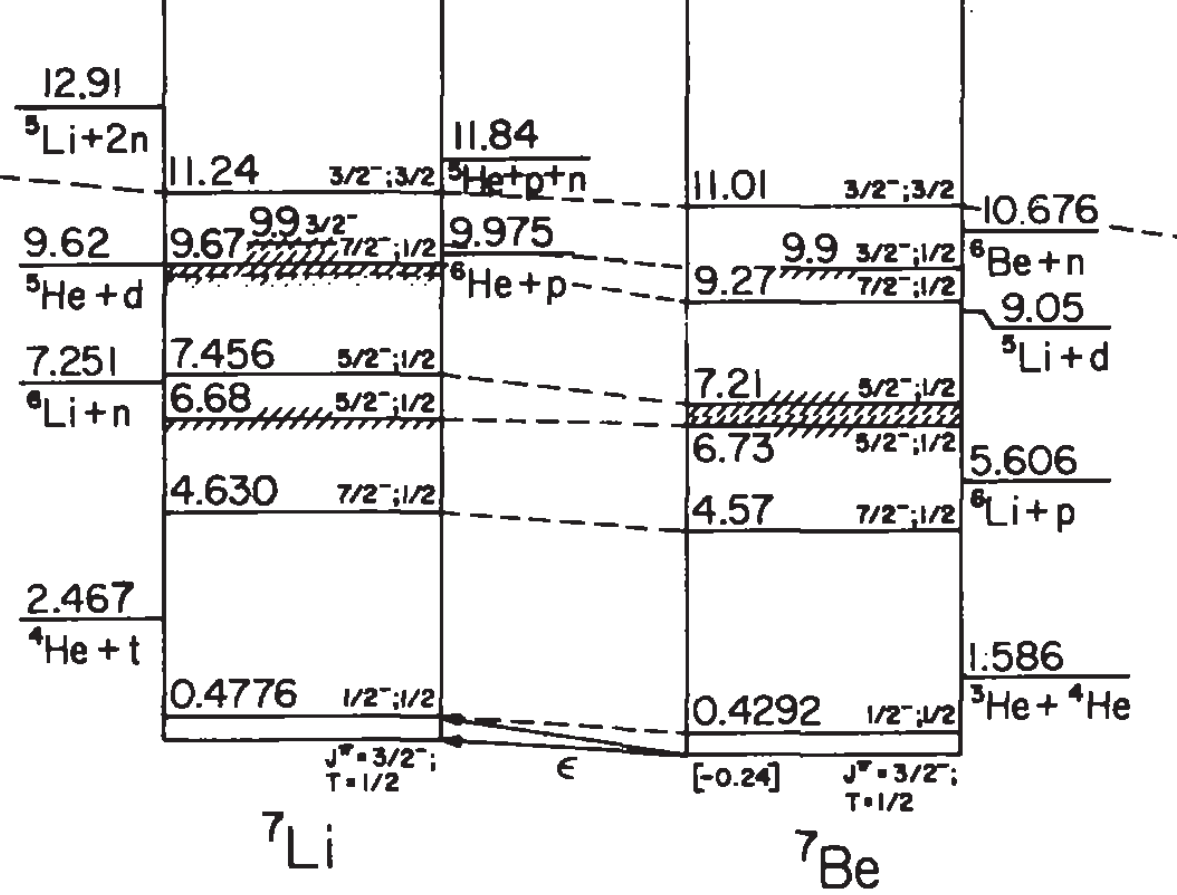
\includegraphics[width=\linewidth]{Imagenes/NivelesEnergiaA7.png}
     \captionof{figure}{Niveles de energía de núcleos con $A=7$.}
     \label{fig: niveles de energia A7}
\end{minipage}
\newpage
\noindent
\begin{minipage}{0.6\textwidth}
    Un ejemplo más ilustrativo son los núcleos con $A=6$ concretamente en $^6\text{He},^6\text{Li},^6\text{Be}$ podemos describir los núcleos como (p,n), por lo tanto tenemos $^6\text{He}=(2,2)+(0,2),^6\text{Li}=(2,2)+(1,1),^6\text{Be}=(2,2)+(2,0)$. Como vemos hay una simetría entre el $^6\text{He}$ y $^6\text{Be}$ ya que hemos cambiado los neutrones por protones respectivamente.
\end{minipage}
\hfill
\begin{minipage}{0.35\textwidth}
    \centering
\begin{tabular}{|ccc|}
\hline
Núcleo        & p & n \\
\hline \hline
$^6\text{He}$ & 2 & 4 \\
$^6\text{Li}$ & 3 & 3 \\
$^6\text{Be}$ & 4 & 2 \\
\hline
\end{tabular}
\captionof{table}{Nucleones dentro de los núcleos con $A=6$.}
\label{tab: Nucleos A6}
\end{minipage}
\\\\ Como la energía de los núcleos es más o menos la misma, la simetría de isospín es \textbf{independiente de la carga}, además la existencia de un estado intermedio como es el $^6\text{Li}$ tenemos que al cambiar protones por neutrones, lo hacemos \textbf{nucleón a nucleón} y no varios a la vez.
\subsection{Analogía de Heisenberg. El espacio de isospín}
En los experimentos de Stern-Gerlach (1922), se observo que en presencia de un campo magnético el electrón se definía en 2 estados y como $2s_e+1=2 \Rightarrow s_e=1/2$. Estos estados correspondían con las proyecciones del spin, $\ket{1/2,1/2},\ket{1/2,-1/2}$.
\\\\
Si recordamos la tabla \ref{tab: Bariones} el neutrón y el protón tienen masas prácticamente iguales y los experimentos nos dicen que ambos tienen la misma $J^p\equiv 1/2^+$, pero hay una pequeña diferencia, y es que mientras que el protón es estable $\tau=\infty$ el neutrón no lo es $\tau=\unit[885.7]{s}$, que se desintegra por el canal débil. Debido a que los núcleos espejos tienen propiedades muy similares, la única interacción que nos queda para explicar esta simetría debe ser la \textbf{interacción fuerte}\footnote{No puede ser débil ya que el neutrón se desintegra y queremos cambiar protones por neutrones y por EM tampoco ya que el neutrón no tiene carga eléctrica.}. \\\\
El neutrón se descubrió en 1932 y en ese mismo año Heisenberg postuló que el protón y el neutrón no eran más que dos posibles estados de una partícula que denominó \textbf{nucleón}. Como había sólo dos posibles estados definió un nuevo número cuántico llamado \textbf{isospín}\footnote{\textit{Spín} de los \textit{isó}topos, spin isotópico.} por lo tanto podemos definir los estados
\begin{equation*}
    2I_N+1=2 \Rightarrow I_N=1/2 \left \{ \begin{aligned}
        &\ket{I\,I_3}=\ket{1/2 , 1/2}\equiv \ket{p}\\
        &\ket{I\,I_3}=\ket{1/2 , -1/2}\equiv \ket{n}
    \end{aligned} \right.
\end{equation*}
Podemos entonces calcular la carga, en unidades de $e$, de los bariones mediante el isospín a través de $Q=I_3+1/2$. Además por ser dos estados de la misma partícula para la interacción fuerte los nucleones tienen la \textbf{misma masa} y son \textbf{indistinguibles} para esta interacción.
\subsubsection{Espacio de isospín}
El isospín se tiene las mismas propiedades que un operador tipo momento angular, por lo tanto el conmutador de sus componentes debe ser $[I_i,I_j]=i\hbar \epsilon_{ijk}I_k$ y como $I^2=\sum^3_i I_i^2$ debe conmutar $[I^2,I_i]=0$, por lo tanto podemos construir los estados igual que en el caso del spin y el momento angular una base que diagonalice en $\qty{I^2,I_3}$.\\\\
Por ser un operador tipo momento angular, los autovalores de los estados propios $\ket{I,I_3}$ son $I^2\ket{I,I_3}=\hbar^2I(I+1)\ket{I,I_3}$ y $I_3\ket{I,I_3}=\hbar I_3\ket{I,I_3}$.\\\\
Supongamos que, al igual que el momento angular total es conservado por el Hamiltoniano de Schrödinger, el isospín lo será para la interacción fuerte, $\qty[H_\mathrm{S},\vec{I}]=0$ y calculamos el elemento de matriz $\mel{I^\prime, I_3^\prime}{H_\mathrm{S}}{I,I_3}$:
\begin{itemize}
    \item Dependencia en la tercera componente $\mel{I, I_3^\prime}{H_\mathrm{S}}{I, I_3}$ $$0=\mel{I, I_3^\prime}{\qty[H_\mathrm{S},I_3]}{I, I_3}=\hbar(I^\prime_3-I_3)\mel{I, I_3^\prime}{H_\mathrm{S}}{I, I_3}\sim \delta_{I_3^\prime I_3}$$
    
    \item Dependencia en el isospín total $\mel{I^\prime, I_3}{H_\mathrm{S}}{I, I_3}$ $$0=\mel{I^\prime, I_3}{\qty[H_\mathrm{S},I^2]}{I, I_3}=\hbar^2(I^\prime (I^\prime+1)-I(I+1))\mel{I^\prime, I_3}{H_\mathrm{S}}{I, I_3}=\hbar^2(I^\prime-I)(I^\prime+I+1)$$ Como el término $I^\prime+I+1$ nunca puede ser 0 necesariamente $I^\prime=I$ por lo tanto $\mel{I^\prime, I_3}{H_\mathrm{S}}{I, I_3}\sim \delta_{I^\prime I}$.

    \item El autovalor del hamiltoniano de la interacción fuerte depende únicamente del isospín total y no sólo de la tercera componente $\mel{I^\prime, I_3^\prime}{H_\mathrm{S}}{I, I_3}$: 
    Como $\qty[H_\mathrm{S}, \vec{I}]=0$ también lo harán los operadores escalera del isospín $\qty[H_\mathrm{S},I_\pm]$, recordamos que al aplicar un operador escalera sobre un estado $I_\pm\ket{I,I_3}=\hbar\sqrt{I(I+1)-I_3(I_3\pm 1)} \ket{I,I_3\pm1}$, por lo tanto $$0=\mel{I,I_ 3}{\qty[H_\mathrm{S},I_+]}{I, I_3-1}\Rightarrow \mel{I,I_3}{H_\mathrm{S}I_+}{I, I_3-1}=\mel{I,I_3}{I_+H_\mathrm{S}}{I, I_3-1}$$ $$\hbar\sqrt{I(I+1)-I_3(I_3- 1)}\mel{I^\prime, I_3^\prime}{H_\mathrm{S}}{I, I_3}=\hbar\sqrt{I(I+1)-I_3(I_3- 1)} \mel{I^\prime, I_3^\prime-1}{H_\mathrm{S}}{I, I_3-1}$$
    $$\mel{I^\prime, I_3^\prime}{H_\mathrm{S}}{I, I_3}=\mel{I^\prime, I_3^\prime-1}{H_\mathrm{S}}{I, I_3-1}$$
    Por lo tanto el elemento de matriz no puede depender de la tercera componente, sólo del isospín total, $\mel{I,I_3}{H_\mathrm{S}}{I,I_3}=A_I $.
\end{itemize}
En conclusión, la interacción fuerte no depende de la tercera componente de isospín, aunque si del isospín total. 
\begin{equation}
    \mel{I^\prime, I_3^\prime}{H_\mathrm{S}}{I,I_3}=A_I\delta_{I^\prime I}\delta_{I_3^\prime I_3}
    \label{eq: elemento de matriz del hamiltoniano fuerte}
\end{equation}
Es decir, una vez especificiado el isospín total, no se distingue entre el protón y el neutrón. Así, calculamos los estados de dos partículas en el espacio de isospín total.

\subsection{Interacción Nucleón-Nucleón. Teorema de Spin-Estadísitca}
Vamos a estudiar cómo interaccionan dos nucleones, para ello conocemos que el isospín total del protón y del neutrón es el mismo $I_1¡=I_2=1/2$ si acoplamos este spin tenemos $\dfrac{1}{2}\otimes \dfrac{1}{2}=0\oplus 1$. Los estados que con acoplamiento a $I=1$
\begin{equation}
\begin{aligned}
    &\ket{11}=\ket{1/2,1/2} \otimes \ket{1/2,1/2} \equiv \ket{pp}\quad \ \ket{1-1}=\ket{1/2,-1/2} \otimes \ket{1/2,-1/2} \equiv \ket{nn}\\
    &\ket{10} =\frac{1}{\sqrt{2}}\qty{\ket{1/2,1/2} \otimes \ket{1/2,-1/2} +\ket{1/2,-1/2} \otimes \ket{1/2,1/2}} \equiv \frac{1}{\sqrt{2}}\qty{\ket{pn}+\ket{np}}
    \label{eq: acoplamientos nucleones isospin 1}
\end{aligned}
\end{equation}

\noindent Si utilizamos la ecuación \ref{eq: elemento de matriz del hamiltoniano fuerte} tenemos que $\mel{11}{H_\mathrm{S}}{11}=\mel{10}{H_\mathrm{S}}{10}=\mel{1-1}{H_\mathrm{S}}{1-1}=A_1$. \\\\
El estado acoplado a $I=0$
\begin{equation}
    \ket{0,0}=\frac{1}{\sqrt{2}}\qty{\ket{1/2,1/2} \otimes \ket{1/2,-1/2} -\ket{1/2,-1/2} \otimes \ket{1/2,1/2}} \equiv \frac{1}{\sqrt{2}}\qty{\ket{pn}-\ket{np}}
    \label{eq: acoplamiento nucleones isospin 0}
\end{equation}
Por lo tanto $\ev{H_\mathrm{S}}{00}=A_0$. Ahora bien, conocemos un estado ligado entre nucleones, el deuterón $pn$, cuál de todos los estados antes escritos describe el deuterón. Si el deuterón lo describe el estado $\ket{10}$ entonces por la simetria de isospín, tenemos que el estado ligado de dos protones y el estado ligado de dos neutrones es posible encontrarlo en la naturaleza, sin embargo hemos demostrado en la sección \ref{sec: estado ligado de dos neutrones} que no es posible un estado ligado de dos neutrones, por lo tanto el deuterón vendrá descrito por la función de onda $\ket{00}$.
\subsubsection{Teorema de spin-estadística e isospín}
El teorema de spin-estadística para fermiones sin isospín nos dice que la función de onda total debe ser antisimétrica $\Psi=\psi(r)\chi_{S}$. Para los estados $\ket{pp},\ket{nn},\ket{pn}$ tenemos que el protón y el neutrón \textbf{son distinguibles}, lo que nos lleva a 

\begin{equation*}
    \begin{aligned}
        & \ket{pp}: \quad L=\mathrm{Par} \Rightarrow \psi(r)=\mathrm{Sim} \left \{ \begin{aligned}
            &S=0 \Rightarrow \chi_S=\text{AntiSim \checkmark}\\
            &S=1 \Rightarrow \chi_S=\text{Sim \XSolidBrush}
        \end{aligned}\right.\\\\
        & \ket{nn}: \quad L=\mathrm{Impar} \Rightarrow \psi(r)=\mathrm{AntiSim} \left \{ \begin{aligned}
            &S=0 \Rightarrow \chi_S=\text{AntiSim \XSolidBrush}\\
            &S=1 \Rightarrow \chi_S=\text{Sim \checkmark}
        \end{aligned}\right.\\\\
        & \ket{pn}: \text{Son distinguibles ya que una esta cargada y otra no y podemos tener }L+S=\text{impar} 
    \end{aligned}
\end{equation*}

 Si ahora incluimos el isospín la función de onda para los fermiones tendrá la forma $\Psi=\psi(r)\chi_{S}\chi_{S}\chi_{I}$, ahora al introducir este grado de libertad, protón y neutrón son \textbf{indistinguibles} desde la interacción fuerte y las funciones de onda serán

\begin{equation*}
    \begin{aligned}
        & \ket{pp}: \ L=\mathrm{Par} \Rightarrow \psi(r)=\mathrm{Sim} \left \{ \begin{aligned}
            &S=0 \Rightarrow \chi_S=\text{AntiSim},I=\text{Impar}\Rightarrow \chi_I=\text{Sim \checkmark}\\
            &S=1 \Rightarrow \chi_S=\text{Sim \XSolidBrush}
        \end{aligned}\right.\\\\
        & \ket{nn}: \ L=\mathrm{Impar} \Rightarrow \psi(r)=\mathrm{AntiSim} \left \{ \begin{aligned}
            &S=0 \Rightarrow \chi_S=\text{AntiSim \XSolidBrush}\\
            &S=1 \Rightarrow \chi_S=\text{Sim}, I=\text{Impar}\Rightarrow \chi_I=\text{Sim \checkmark}
        \end{aligned}\right.\\\\
        & \ket{pn}: \text{La función de onda total debe ser antisimétrica.}\\
        & \underbrace{L+S}_{\text{Impar}}= \left \{\begin{aligned}
            &L=\text{Par} \Rightarrow \psi(r)=\text{Sim}, S=1\Rightarrow \chi_S=\text{Sim}, I=0 \Rightarrow \chi_I=\text{AntiSim \checkmark}\\
            &L=\text{Impar} \Rightarrow \psi(r)=\text{AntiSim}, S=0\Rightarrow \chi_S=\text{AntiSim}, I=0 \Rightarrow \chi_I=\text{AntiSim \checkmark}
        \end{aligned} \right.
    \end{aligned}
\end{equation*}

\noindent Por lo tanto tenemos que la restricción del principio de exclusión de Pauli será $L+S+I=$impar
\subsection{Relación de Gell-Mann-Nishijima. Asignación de isospín al resto de hadrones}
\subsubsection{\underline{Materia Nuclear Ordinaria}}
El isospín no está reservado únicamente para los nucleones, si nos fijamos en los piones (mediadores de la interacción nuclear) también tienen isospín. Si recordamos el pion tiene por estados 
\begin{equation*}
    \begin{aligned}
        &\pi^0 \quad J^\pi=0^-  \quad m_{\pi^0}=\unit[134.979]{MeV/\textit{c}^2} \\
        &\pi^\pm \quad J^\pi=0^- \quad m_{\pi^\pm}=\unit[139.570]{MeV/\textit{c}^2}
    \end{aligned}
\end{equation*}
Al igual que para le neutrón y el protón la diferencia de masas se debe a las correcciones electromagnéticas ya que difieren en la segunda cifra significativa. Se diferencian en carga y en su vida media ya que mientras que el pión neutro se desintegra por EM; los piones cargados se desintegran por débil.\\\\
Ahora bien, como la interacción fuerte no distingue la carga tenemos 3 posibles estados
\begin{equation*}
    \pi^{\pm,0}\Rightarrow 2I_\pi+1=3\Rightarrow I_\pi=1 \Rightarrow \left \{ \begin{aligned}
        &\ket{11}=\pi^+ \\
        & \ket{10}=\pi^0\\
        &\ket{1-1}=\pi^-
    \end{aligned}\right.
\end{equation*}
Como ya hemos hecho para los nucleones, queremos relacionar la tercera componente de isospín con la carga de los piones, en este caso se corresponde con $Q=I_3$. Esta asignación también la hacemos para los mesones $\rho^{0,\pm}$\\\\
Vamos a estudiar el caso del cuadruplete $\Delta$, como tenemos 4 posibles estados tendremos que el isospín de esta partícula será
\begin{equation*}
    \Delta^{++,+,0,-}\Rightarrow 2I_\Delta+1=4 \Rightarrow I_\Delta=\frac{3}{2} \Rightarrow \left \{ \begin{aligned}
        & \ket{3/2,+3/2}=\Delta^{++} \\
        & \ket{3/2,+1/2}=\Delta^{+}  \\
        & \ket{3/2,-1/2}=\Delta^{0}  \\
        & \ket{3/2,-3/2}=\Delta^{-}  
    \end{aligned}\right.
\end{equation*}
Que tendría como relación de carga e isospín $Q=I_3+\dfrac{1}{2}$ (la misma que para los nucleones), por lo que podemos establecer que esa relación es válida para los bariones mientras que la que hemos deducido del pión será válida para los meones. Tanto nucleones, como $\Delta$'s, como $\pi$'s pertencen a la \textbf{materia nuclear ordinaria}, es decir, el único sabor distinto de 0 es el del número bariónico y podemos obtener la \textbf{relación de Gell-Mann-Nishijima} para materia nuclear ordinaria:
\begin{equation}
    \boxed{\frac{Q}{e}=I_3+\frac{B}{2}}
    \label{eq: Relacon de Gell-Mann Nishijima sin extrañeza}
\end{equation}
\newpage
\subsubsection{Consecuencias y validez de la simetría de isospín}
Vamos a estudiar dos ejemplos, el primero tenemos veremos reacciones pión nucleón\\\\
\noindent
\begin{minipage}{0.45\textwidth}
Tenemos ocho procesos diferentes en las interacciones pión nucleón:

    \begin{equation*}
    p + \pi^+ \longrightarrow p + \pi^+
\end{equation*}
\begin{equation*}
    p + \pi^- \longrightarrow p + \pi^-, \, n + \pi^0
\end{equation*}
\begin{equation*}
    p + \pi^0 \longrightarrow p + \pi^0, \, n + \pi^+
\end{equation*}
\begin{equation*}
    n + \pi^- \longrightarrow n + \pi^-
\end{equation*}
\begin{equation*}
    n + \pi^+ \longrightarrow p + \pi^0, \, n + \pi^+
\end{equation*}
\begin{equation*}
    n + \pi^0 \longrightarrow n + \pi^0, \, p + \pi^-
\end{equation*}

\end{minipage}
\hfill
\begin{minipage}{0.45\textwidth}
    Si estudiamos los acoplamientos de isospín, como el isospín del pion es $I_\pi=1$ y $I_N=\dfrac{1}{2}$ tenemos que 
    \begin{equation*}
        1\otimes \frac{1}{2}=\frac{1}{2}\oplus \frac{3}{2}
    \end{equation*}
    Y recordando la ecuación \ref{eq: elemento de matriz del hamiltoniano fuerte} tenemos:
    \begin{equation*}
        \begin{aligned}
            & \ev{H_\mathrm{S}}{3/2 I_3}=A_{1/2}\\
            & \ev{H_\mathrm{S}}{3/2 I_3}=A_{3/2}
        \end{aligned}
    \end{equation*}    
\end{minipage}\\\\
\noindent
Los ocho procesos están descritos únicamente por dos cantidades linealmente independientes. 
\\\\
Estudiemos ahora la generación de piones en un scattering protón$\equiv \ket{1/2,1/2}$ deuterón$\equiv \ket{00}$, en este caso tenemos dos canales de desintegración
\begin{equation*}
    \begin{aligned}
        &p+d\longrightarrow \,^3\text{He}+\pi^0 \\
        &p+d\longrightarrow \,^3\text{H}+\pi^+
    \end{aligned}
\end{equation*}
En el estado inicial tenemos que $\ket{i}\equiv \ket{1/2,1/2}\otimes \ket{00}=\textcolor{red}{\braket{\frac{1}{2}0\frac{1}{2}0}{\frac{1}{2}\frac{1}{2}}}\ket{\frac{1}{2}\frac{1}{2}}=\textcolor{red}{1}\ket{\frac{1}{2}\frac{1}{2}}$. Ahora queremos calcular el la función de onda en el estado final, el isospín del $^3\text{He}$ es $I_3(^3\text{He})=\dfrac{1}{2}$ y la función de onda ha de ser
\begin{equation*}
\ket{\pi^0\, ^3\text{He}}=\ket{10}\otimes\ket{\frac{1}{2} \frac{1}{2}}=\braket{10\frac{1}{2} \frac{1}{2}}{\frac{1}{2}\frac{1}{2}}\ket{\frac{1}{2}\frac{1}{2}}+\braket{10\frac{1}{2} \frac{1}{2}}{\frac{3}{2}\frac{1}{2}}\ket{\frac{3}{2}\frac{1}{2}}=-\sqrt{\frac{1}{3}} \ket{\frac{1}{2}\frac{1}{2}}+\sqrt{\frac{2}{3}}\ket{\frac{3}{2}\frac{1}{2}}
\end{equation*}

\noindent El tritio tiene proyección de isospín  $I_3(^3\text{H})=-\dfrac{1}{2}$ y la función de onda del estado final es 
\begin{equation*}
    \ket{\pi^0\, ^3\text{H}}=\ket{11}\otimes\ket{\frac{1}{2} -\frac{1}{2}}=\braket{11\frac{1}{2} -\frac{1}{2}}{\frac{1}{2}\frac{1}{2}}\ket{\frac{1}{2}\frac{1}{2}}+\braket{11\frac{1}{2} -\frac{1}{2}}{\frac{3}{2}\frac{1}{2}}\ket{\frac{3}{2}\frac{1}{2}}=\sqrt{\frac{2}{3}} \ket{\frac{1}{2}\frac{1}{2}}+\sqrt{\frac{1}{3}}\ket{\frac{3}{2}\frac{1}{2}}
\end{equation*}
Ahora comparemos las secciones eficaces de cada scattering
\begin{equation*}
    R=\frac{\sigma(p+d\xrightarrow{} \,^3\text{He}+\pi^0 )}{\sigma (p+d\xrightarrow[]{} \,^3\text{H}+\pi^+)}= \frac{\mel{\pi^0\, ^3\text{He}}{H_\mathrm{S}}{pd}}{\mel{\pi^0\, ^3\text{H}}{H_\mathrm{S}}{pd}}
\end{equation*}

Los elementos de matriz son
\noindent

\begin{minipage}{0.65\textwidth}
    \begin{equation*}
    \begin{aligned}
        &\mel{\Pi^0 \; ^3\text{He}}{H_\mathrm{S}}{p d} = 
\qty( - \sqrt{\frac{1}{3}} \bra{\frac{1}{2} +\frac{1}{2}} + \sqrt{\frac{2}{3}} \bra{\frac{3}{2} +\frac{1}{2}} ) H_\mathrm{S} \ket{\frac{1}{2} +\frac{1}{2}} \\&= - \sqrt{\frac{1}{3}} \bra{\frac{1}{2} +\frac{1}{2}} H_\mathrm{S} \ket{\frac{1}{2} +\frac{1}{2}} + \sqrt{\frac{2}{3}} \bra H_\mathrm{S} \ket{\frac{1}{2} +\frac{1}{2}}= - \sqrt{\frac{1}{3}} A_{1/2}
    \end{aligned}
\end{equation*}
\end{minipage}
\hfill
\begin{minipage}{0.25\textwidth}
     $$\mel{\pi^0\, ^3\text{H}}{H_\mathrm{S}}{pd}=\displaystyle \sqrt{\dfrac{2}{3}}A_{1/2}$$ y por lo tanto $R=\dfrac{1}{2}$
\end{minipage}\newpage
Es decir, solamente sabiendo que $\qty[H_\mathrm{S},\vec{I}]=0$ hemos sido capaces de conocer relaciones entre las secciones eficaces. 
\subsubsection{\underline{Materia nuclear extraña}}
En el siguiente proceso , fuerte
\begin{equation}
    \pi^- +p\longrightarrow K^0+\Lambda
    \label{eq: absorcion pion por proton}
\end{equation}
Las partículas extrañas se desintegran a través de interacción débil como
$$\begin{aligned}
    &K^0 \longrightarrow \pi^++\pi^-\\
    &\Lambda \longrightarrow p+\pi^-
\end{aligned}$$
Ahora vamos a determinar el isospín del barión $\Lambda$, como sólo hay una, tenemos que $2I_\Lambda+1=1$ y por lo tanto $I_\Lambda=0$. Si buscamos la relación entre la carga eléctrica y la tercera componente de isospín es $Q=I_3$. \\\\Para el isospín del $K^0$, podríamos pensar que sucede igual que para los piones, pero no se conserva el isospín, por lo tanto lo estudiaremos a partir de la reacción \ref{eq: absorcion pion por proton}
\begin{equation*}
    \begin{aligned}
        & \quad \quad \quad \pi^- +p\longrightarrow K^0+\Lambda\\
        &I: \quad \quad 1 \quad  \frac{1}{2} \longrightarrow \boxed{\frac{1}{2},\frac{3}{2}} \quad 0 \\
        & I_3: \quad -1 \quad \frac{1}{2} \longrightarrow  I_3(K^0) \quad  0
    \end{aligned}
\end{equation*}
Ahora bien, como la tercera componente de isospín es conservada y se calcula de manera algebraica, $I_3(K^0)=-\dfrac{1}{2}$, pero cuál es el isospín total del kaón neutro, si suponemos que tenemos $I_{K^0}=\dfrac{3}{2}$ deberían existir kaones doblemente cargados ya que habría 4 estados ($\Delta$'s) y no existen mesones doblemente cargados, además si nos adentramos en el modelo quark, como los mesones están compuestos por dos quarks, es imposible alcanzar cargas mayores a 1 con sólo dos quarks. \\\\Por lo tanto el isospín total del kaón es $I_{K^0}=\dfrac{1}{2}$,Por lo tanto tenemos que sólo hay $2I_{K}+1=2$ estados, $(K^0,K^+)$ y la relación de isospín y carga para los kaones es $Q=I_3+\dfrac{1}{2}$. Pero conocemos un estado con carga negativa del kaón, para solucionarlo suponemos que existe otro doblete que sea $K^-,K^0_?$ que para este caso la relación carga isospín será $Q=I_3-\dfrac{1}{2}$.\\\\
Si recordamos la ecuación \ref{eq: Relacon de Gell-Mann Nishijima sin extrañeza}, vemos que ni el barión lambda ni el kaón la satisfacen, pero los nucleones y los piones son materia nuclear ordinaria, no extraña. Esto lo podemos solucionar si definimos la \textbf{hipercarga} como  $Y=B+S$, obteniendo finalmente la \textbf{relación de Gell-Mann Nishijima} 
\begin{equation}
    \boxed{Q=I_3+\frac{Y}{2}}
    \label{eq: Relacion de Gell-Mann nishijima}
\end{equation}
\newpage
\section{Propiedades fundamentales de la interacción fuerte}
Con todo lo introducido anteriormente, podemos establecer una clasificación de las partículas que son producidas en reacciones fuertes y decaen por interacción débil y electromagnética., de acuerdo a su isospín, extrañeza, número bariónico. Tenemos



\begin{table}[h!]
    \centering
    \setlength{\tabcolsep}{10pt}
    \begin{tabular}{|c|c|c|c|c|c|c|c|c|}
        \hline
        \textbf{B} & \textbf{S} & \textbf{I} & \multicolumn{5}{c|}{$I_3$} & \textbf{Masa} \\
        \cline{4-8}
        & & & -1 & -1/2 & 0 & 1/2 & 1 & \\
        \hline
        1 & 0 & $\frac{1}{2}$ & & $n$&  & $p$ &  & 939 \\
        \hline
        1 & -1 & 0 & & & $\Lambda$ & & & 1116 \\
        \hline
        0 & 0 & 1 & $\pi^-$ & & $\pi^0$ & & $\pi^+$ & 139 \\
        \hline
        0 & +1 & $\frac{1}{2}$ & & $K^0$ & & $K^+$ & & 495 \\
        \hline
        0 & -1 & $\frac{1}{2}$ &  & $K^-$ &  & $\bar{K}^0$ & & 495 \\
        \hline
        1 & -1 & 1 & $\Sigma^-$ & & $\Sigma^0$ & & $\Sigma^+$ & \begin{tabular}{c} 1197 \\ 1192 \\ 1189 \end{tabular} \\
        \hline
        1 & -2 & $\frac{1}{2}$ & & $\Xi^0$ &  & $\Xi^-$ & & \begin{tabular}{c} 1318 \\ 549 \end{tabular} \\
        \hline
        1 & -3 & 0 & & & $\Omega^-$ & & & $**$ \\
        \hline
        0 & 0 & 0 & & & $\eta$ & & & 549 \\
        \hline
    \end{tabular}
    \caption{Clasificación de partículas producidas por reacciones fuertes.}
    \label{tab: particulas producidas por reacciones fuertes}
\end{table}

La conservación de todos estos números cuánticos en procesos fuertes nos da información de la naturaleza de algunos decaimientos como es el caso de los bariones $\Sigma^+\xrightarrow{} n+\pi+,$  $\Xi^-\xrightarrow[]{} \Lambda+\pi^-$ que lo hacen por débil ya que no conservan extrañeza, ó $\Sigma^0\xrightarrow[]{} \Lambda+\gamma$ que lo hace por electromagnética.\\\\
Una propiedad interesante por de esta tabla es que si seguimos la misma fila, están degeneradas para la interacción fuerte. Ésto nos permite construir multipletes de isospín.
\begin{figure}[h]
    \centering
    % Primera subfigura
    \begin{subfigure}[h]{0.3\textwidth}
        \centering
        \includegraphics[scale=0.65]{Diagramas Tema 2/DGellmanJP=0-.pdf}
        \caption{Partículas $J^P=0^-$}
    \end{subfigure}
   \hfill
    % Segunda subfigura
    \begin{subfigure}[h]{0.3\textwidth}
        \centering
        \includegraphics[scale=0.65]{Diagramas Tema 2/DGellManJP=1_2+.pdf}
         \caption{Partículas $J^P=\dfrac{1}{2}^+$}
    \end{subfigure}
    \hfill % Espacio entre subfiguras
    % Tercera subfigura
    \begin{subfigure}[h]{0.3\textwidth}
        \centering
        \includegraphics[scale=0.65]{Diagramas Tema 2/DGellManJP=3_2+.pdf}
        \caption{Partículas $J^P=\dfrac{3}{2}^+$}
    \end{subfigure}
    \label{fig: diagramas de gellmann}    
    \caption{Representaciones irreducibles de los bariones y los mesones con quarks ligeros.}
\end{figure}

Si representamos estos diagramas en un plano cartesiano $(I_3,Y)$ si nos movemos por las líneas alcanzaremos todos los hadrones.

\newpage
\subsection{Hipótesis de los tres quarks ligeros. (Otra vez)}

Si recordamos la sección \ref{subsec: hipotesis tres quarks ligeros}, Gell-Mann postuló que las partículas fundamentales estaban constituidas por un doblete $u,d$ y un singlete $(s)$ cuyos elementos denominó quarks. 
\\\\
Los quarks y los antiquarks los podemos tienen una representación fundamental
\begin{figure}[h]
    \begin{subfigure}{0.45\textwidth}
        \centering
        \includegraphics[width=0.65\textwidth]{Diagramas Tema 2/RepreIrreducibleQuark.pdf}
        \caption{Representación irreducible del doblete $(u,d)$ y el singlete $(s)$.}
        \label{fig: Representacion irreducible quark}
    \end{subfigure}
    \hfill
        \begin{subfigure}{0.45\textwidth}
        \centering
        \includegraphics[width=0.65\textwidth]{Diagramas Tema 2/RepreIrreducibleAntiQ.pdf}
        \caption{Representación irreducible del doblete $(\bar{u},\bar{d})$ y el singlete $(\bar{s})$.}
        \label{fig: Representacion irreducible antiquarks}
    \end{subfigure}
    \caption{Representaciones irreducibles de quarks y antiquarks}
\end{figure}

Así podemos efectuar la asignación de quarks tanto a los bariones como a los mesones.
\subsubsection{Diagramas de Quarks}
Las reacciones perrmitidas por interacción fuerte se pueden dibujar fácilmente en términos de diagramas de quarks. La si tenemos las desintegraciones de la $\Delta^{++}$
$$\Delta^{++}\longrightarrow \pi^++p \hspace{2cm} \Delta^{++}\longrightarrow \pi^++\pi^+ $$

Si los representamos en diagramas de quarks ambas reacciones serán
\begin{figure}[h]
    \centering
    \begin{subfigure}{0.45\textwidth}
        \centering
        \includegraphics[width=0.65\textwidth]{Diagramas Tema 2/DiagramadeQuarksDelta++Posible.pdf}
        \caption{Diagrama de quarks de $\Delta^{++}\xrightarrow[]{} \pi^++p$.}
        \label{fig: diagrama de quarks delta ++ posible}
    \end{subfigure}
    \hfill
        \begin{subfigure}{0.45\textwidth}
        \centering
        \includegraphics[width=0.65\textwidth]{Diagramas Tema 2/DiagramaQuarksDelta++imposible.pdf}
        \caption{Diagrama de quarks de $\Delta^{++}\xrightarrow[]{} \pi^++\pi^+$.}
        \label{fig: diagrama de quarks delta ++ imposible}
    \end{subfigure}
    \caption{Diagramas de quarks}
    \label{fig:diagramas posibles e imposibles}
\end{figure}

Por lo tanto si en el diagrama no podemos seguir las líneas fermiónicas la reacción no podrá darse.

\subsubsection{Estados exóticos}
Como ya hemos mencionado tenemos las estructuras más sencillas de los quarks son los mesones $(q\bar{q})$ y los bariones $(qqq)$. La extrañeza y la carga pueden tomar valores\\\\
\noindent
\begin{minipage}{0.45\linewidth}
    \centering
\begin{tabular}{|cc|}
\hline
\textit{S} & \textit{Q} \\
\hline \hline
-3         & -1         \\
-2         & -1,0       \\
-1         & -1,0,+1    \\
0          & -1,0,+1,+2 \\
\hline
\end{tabular}
\captionof{table}{Valores posibles de carga y extrañeza para los bariones.}
\label{tab: cargay y extraeza bariones}
\end{minipage}
\hfill
\begin{minipage}{0.45\linewidth}
    \centering
\begin{tabular}{|cc|}
\hline
\textit{S} & \textit{Q} \\
\hline \hline
-1         & -1,0       \\
0          & -1,0,+1    \\
1          & 0,+1      \\
\hline
\end{tabular}
\captionof{table}{Valores posibles de carga y extrañeza para los mesones.}
\label{tab: cargay y extraeza mesones}
\end{minipage}
\\\\
Por lo tanto todas las partículas que no satisfagan estas reacciones reciben el nombre de \textbf{estados exóticos}, siempre que puedan existir en la naturaleza, un ejemplo es el pentaquark $\Theta^+(1540)$ que tiene $B=1, S=+1, Q=+1$, que tiene por estructura $(\bar{s}dduu)$. Tras encontrar esta partícula, se demostró que no existe en $\unit[1540]{MeV}$.
\subsection{Color}
El modelo de Gell-Mann tenía un problema fundamental: contradecía toda la física conocida hasta el momento.\\\\
Por ejemplo el barión $\Delta^{++}(uuu)$ viola el principio de exclusión de Pauli \footnote{\textbf{Notación}: Los quarks en máxima componente de spin los denotamos como $\uparrow$ mientras que los que tengan mínima componente $\downarrow$}, conocemos que el spin de la partíucula es $J=3/2 \Rightarrow s=3/2$. Si escogemos el quark $\Delta^{++}(\uparrow \uparrow)\equiv S_z=3/2$ necesariamente los tres quarks deben ser $u \uparrow$, por lo tanto la función de onda en el espacio de sabor del $\Delta^{++}$ será $$\Psi_{\Delta^{++}}=u\uparrow u\uparrow u\uparrow \xrightarrow[]{} \chi_S=\text{simétrica\footnotemark}$$
\footnotetext{Es simétrica por ser el acoplamiento de \textbf{máxima componente} de momento angular, que para tres partículas es la única que está determinada de manera unívoca.}
Como son estados ligeros, deben estar en onda $S, (\ell=0) \xrightarrow[]{} \psi_r=\text{simétrica}$. Por lo tanto el espacio de sabor de la función de onda es simétrica, lo que viola el principio de exclusión de Pauli, pero sí que se observa en la naturaleza. Para ello introducimos un nuevo número cuántico para antisimetrizar la función de onda, como hicieron Stern y Gerlach con el spín.\\\\
Greenberg (1964) postuló la existencia de un nuevo número cuántico al que llamó color. Éste número cuántico debía arreglar el poblema de la $\Delta^{++}$, y por tanto necesitamos al menos 3 grados de libertad. Para ello asignamos un estado diferente a cada uno de los quarks de manera que la función de onda sea totalmente antisimétrica, a estos estados los llamamos: rojo $R$, verde $G$ y azul $B$ en analogía a la teoría óptica del color. La simetría de color presenta las siguientes propiedades
\newpage
\begin{itemize}
    \item \textbf{Confinamiento}: El color \textbf{no existe} libre en la naturaleza, por lo tanto todas las partículas deben ser blancas $R+G+B$.
    \item \textbf{Tres colores}: La función de onda debe ser antisimétrica.
    \item \textbf{Sólo es simetría de la interacción fuerte}: Solo los quarks tienen color. El color de un antiquark es el \textbf{anticolor}.
\end{itemize}

Ahora podemos estudiar cuántas partículas podemos obtener en la hipótesis de los tres quarks ligeros de Gell-Mann. Si denotamos como $\alpha$, $\beta$, $\gamma$ a las posibles partículas, tenemos tres posibles configuraciones:
\begin{itemize}
    \item $\alpha \beta \gamma$: Sólo conocemos una posible configuración $(uds)\equiv \Lambda, \Sigma^0$. Acoplando los momentos angulares
    $$\alpha \beta=\frac{1}{2}\otimes \frac{1}{2} \Rightarrow \left \{ \begin{aligned}
        0 \otimes \frac{1}{2}= \frac{1}{2} \\\\ 1\otimes \frac{1}{2} = \frac{1}{2},\frac{3}{2}
    \end{aligned}\right. $$
    Donde el último acople a $\dfrac{1}{2}$ se debe al acoplo con $\gamma$.
\item $\alpha \alpha \beta$: La función de onda de color es antisimétrica, por lo tanto la función de onda radial y la de isospín  de las $\alpha$ debe ser simétrica $\ell,I=1$. Así $$\alpha \alpha =1 \Rightarrow \left \{ \begin{aligned}
     \frac{1}{2} \\\\ \frac{3}{2}
    \end{aligned}\right. $$
Para las cuales tenemos seis posibles combinaciones $(uud),(uus),(ddu),(dds),(ssu),(ssd)$.
\item $\alpha \alpha \alpha$: Para este caso sólo tenemos 3 combinaciones posibles $(uuu), (ddd), (sss)$ y todas han de tener acoplo a máxima componente por lo tanto $J=3/2$
\end{itemize}
En total podemos tener 8 partículas de spin $1/2$ y 10 partículas de spin $3/2$ que coincide con los diagramas \ref{fig: diagramas de gellmann}
\subsubsection{¿Cuántos colores hay? Hipótesis del color}
Tenemos las siguientes reacciones en una colisión electrón-positrón, estas reacciones son electromagnéticas
\begin{equation*}
    \left \{ \begin{aligned}
         &e^++e^-\longrightarrow \mu^++\mu^- \\
         &e^++e^-\longrightarrow q+\bar{q} \xrightarrow[]{} \text{hadrones}
    \end{aligned} \right.
\end{equation*}
Con secciones eficaces $\sigma(e^++e^- \xrightarrow[]{} \mu^++\mu^-))=\dfrac{\pi}{8}\dfrac{\alpha^2}{E^2}$ , $\sigma(e^++e^- \xrightarrow[]{} \text{hadrones}))= \displaystyle\sum_a e^2_a\dfrac{\pi}{8}\dfrac{\alpha^2}{E^2}$, donde en esta última no hemos tenido en cuenta el color y $a$ son los sabores $u,d,c,s,b$ de los distintos quarks y $e_a$ su respectiva carga en unidades de la carga fundamental.\\\\
 La razón entre las secciones eficaces es $$R=\sum_a e^2_a=\qty(\dfrac{2}{3})^2+\qty(-\dfrac{1}{3})^2+\qty(\dfrac{2}{3})^2+\qty(-\dfrac{1}{3})^2+\qty(-\dfrac{1}{3})^2=\dfrac{11}{9}\sim 1$$ lo cual iba en contra de los experimentos que decían que la razón debía ser $R_\text{exp}\lesssim 4$, que es lo que obtenemos si tenemos en cuenta el color ya que $R=N_\mathrm{c} \dfrac{11}{9} \lesssim 4 \Rightarrow N_\mathrm{c}=3$
 \subsection{Diferencia de masa de multipletes}
  En un diagrama de Gell-Mann las \textbf{líneas de isospín} (verticales) son de origen electromagnético. La masa de una partícula viene dada por la masa constituyente (masa de todas las particulas que la forman), y los términos de acoplamiento fuerte y electromagnético. Por ejemplo para el caso de los bariones $\Sigma^+(1189),\Sigma^0 (1193), \Sigma^-(1197)$ tenemos:
\begin{equation*}
\begin{aligned}
    M(\Sigma^-) &= 2m_d + m_s + \cancelto{A}{\mel{1 -1}{H_\mathrm{S}}{1 -1}} + \cancelto{\frac{\delta}{3}}{\dfrac{1}{9}\delta + 2 \dfrac{1}{9}\delta} \\
    M(\Sigma^0) &= m_u + m_d + m_s + \cancelto{A}{\mel{1 0}{H_\mathrm{S}}{1 0}} + \cancelto{-\frac{\delta}{3}}{\dfrac{1}{9}\delta + 2 \dfrac{2}{3} \qty(-\dfrac{1}{3}) \delta} \\
    M(\Sigma^+) &= 2m_u + m_s +\cancelto{A}{\mel{1 1}{H_\mathrm{S}}{1 1}} + \cancelto{0}{\dfrac{4}{9}\delta + 2 \dfrac{2}{3} \qty(-\dfrac{1}{3}) \delta}
\end{aligned}
\end{equation*}

\noindent Manipulando un poco estas expresiones llegamos a que la diferencia entre las masas $$m_d-m_u=\dfrac{1}{3}\qty[M(\Sigma^-)+M(\Sigma^0)-2M(\Sigma^+)]=\unit[3.78]{MeV}$$
Si estudiamos la diferencia de masas entre las partículas de una misma línea de hipercarga (lado izquierdo del diagrama de Gell-Mann \ref{fig: diagramas de gellmann}) vemos que el resultado es aproximadamente constante $$\underbrace{\Sigma^*(1384)-\Delta(1232)}_{\unit[152]{MeV}}\approx \underbrace{\Xi^*(1533)-\Sigma^*(1384)}_{\unit[149]{MeV}}\approx \underbrace{\Omega^--\Xi^*(1533)}_{\unit[139]{MeV}}$$ Esto nos peremite estimar la masa del quark $s$ es $m_s=m_u+\delta$ y por ello Gell-Man dividió sus quarks en un doblete y un singlete. Si nos movemos alrededor de las líneas de hipercarga, estamos cambiando un quark extraño por uno ligero y por tanto tenemos que $m_s-m_{u,d}\approx \unit[150]{MeV}$.\\\\ Fue la última igualdad la que permitió a Gell-Mann postular que debía existir una partícula con extrañeza -3 y como se conocía su masa tan sólo hubo que alcanzar dichas energías en la colisión para que Gell-Mann obruviera el premio Nobel en 1969.
\subsubsection{¿Por qué tienen distinta masa los bariones de $J=1/2$ y $J=3/2$?}
El orgígen de la diferencia de masa entre los multipletes están en el acoplamiento de spin de la partícula.\newpage
Si recordamos los niveles de energía atómicos tenían correcciones más allá del potencial coulombiano, las correcciones que corresponden las interacciones de los  spines de los núcleos con el spin de los electrones se conocen como \textbf{correcciones hiperfinas}.\\\\
La interacción entre fermiones cargados viene dada por el \textbf{potencial de Breit-Fermi}, este potencial a primer orden tiene un término coulombiano y a segundo orden introduce el término que depende del spin de las partículas por ello si suponemos que nos encontramos en un estado de onda S
\begin{equation}
H_{SS}=k\sum_{i<j}    \frac{\vec{s}_i\cdot \vec{s}_j}{m_im_j}
\label{eq: potencial de fermi-breit}
\end{equation}
En materia nuclear ordinaria (los quarks $u$ y $d$ tienen más o menos la misma masa) el potencial de interacción será 
\begin{equation*}
    H_{SS}=\frac{k}{m^2}\qty(\vec{s}_1\cdot \vec{s}_2+\vec{s}_1\cdot \vec{s}_3+\vec{s}_3\cdot \vec{s}_3)=\frac{k}{2m^2}\qty(\underbrace{\qty(\vec{s}_1+\vec{s}_2+\vec{s}_3)^2}_{J^2}-\vec{s}_1^{\,2}-\vec{s}_2^{\,2}-\vec{s}_3^{\,2})
\end{equation*} 
Si calculamos el valor esparado de este pootencial obtenemos 
\begin{equation*}
    \expval{H_{SS}}=\frac{k}{2m^2}\qty(J(J+1)-\frac{9}{4})\Rightarrow \left \{ \begin{aligned}
        & \mathrm{Octete} \ (J=\nicefrac{1}{2}) \xrightarrow{} -\nicefrac{3}{4}\\
        & \mathrm{Decuplete} \ (J=\nicefrac{3}{2}) \xrightarrow{} \nicefrac{3}{4}
    \end{aligned} \right. \times \frac{k}{2m^2}
\end{equation*}
Así podemos sacar la diferencia de masas entre deltas y nucleones: $M_\Delta-M_N= \dfrac{3}{2}\dfrac{k}{m^2}=\unit[292]{MeV}$.
\subsection{Propiedades del potencial de la interacción fuerte}
Vamos a estudiar ahora la diferencia de masa entre las partículas ${\Sigma^+}^*(uus),\Sigma(uds),\Lambda(uds)$, que tienen por spin total $\nicefrac{3}{2},\nicefrac{1}{2},\nicefrac{1}{2}$, respectivamente.  estos hiperones tienen un doblete de quarks $uu,ud$, este doblete lo denotaremos como $\vec{s}_d=\vec{s}_2+\vec{s}_3$.\\\\
Las funciones de onda de color siempre son antisimétricas. Para el doblete ligero en los $\Sigma$'s tendremos que tanto la función de onda radial (onda S) como la de sabor (el intercambio $u\leftrightarrow u, u \leftrightarrow d$) son simétricas , por lo que el spin debe de ser simétrica y $s_d=1$. Para el caso de la $\Lambda$ tenemos que la función de onda de sabor es antisimétrica por ser ortogonal a $\Sigma$ y por ende la función de onda de spin debe serlo también por lo que en este caso $s_d=0$.
\\\\
El potencial de interacción dentro de los hiperones en este caso es
\begin{equation*}
    H_{SS}=\frac{k}{m_u^2}\qty(\vec{s}_2\cdot \vec{s}_3)+\frac{k}{m_um_s}\qty(\vec{s_1}\cdot \vec{s_d})=\frac{k}{2m_u^2}\qty({\vec{s}_d}^{\,2}-{\vec{s}_2}^{\,2}-{\vec{s}_3}^{\,2})+\frac{k}{2m_um_s}\qty(J^2-{\vec{s}_d}^{\,2}-{\vec{s}_1}^{\,2})
\end{equation*}
Y su valor esperado
\begin{equation*}
    \expval{H_{SS}}=\frac{k}{m_u^2}\qty(s_d(s_d+1)-\frac{3}{2})+\frac{k}{m_um_s}\qty(J(J+1)-s_d(s_d+1)-\frac{3}{4}) \Rightarrow
\end{equation*}
$$\expval{H_{SS}}=\mqty({\Sigma^+}^* \\ \Sigma \\ \Lambda)=\frac{k}{4m_u^2}\mqty(1 \\1 \\-3)+\frac{k}{2m_um_s}\mqty(1\\-2\\0)$$

Con lo que podemos calcular las diferencias de masa
\begin{equation*}
    \begin{aligned}
        &M_{\Sigma^*}-M_{\Sigma^0}=\frac{3}{2}\frac{k}{m_um_s}=\delta_{N\Delta}\frac{m_u}{m_s} \\
        &M_{\Sigma^0}-M_{\Lambda}= \frac{k}{m_u^2}-\frac{k}{m_um_s}=\frac{2}{3 }\delta_{N\Delta}\qty[1-\frac{m_u}{m_s}]\\
        &M_{\Sigma^*}-M_{\Lambda}=\frac{k}{m_u^2}+2\frac{k}{m_um_s}=\frac{2}{3 }\delta_{N\Delta}\qty[1+\frac{m_u}{m_s}]
    \end{aligned}
\end{equation*}

Como $\delta_{N\Delta}=M_\Delta-M_N=\unit[292]{MeV}$ y ajustando datos experimentales obtenemos que $\dfrac{m_u}{m_s}=0.64$ podemos predecir el incremento de las masas de todas las partículas que quisiéramos, por lo tanto tenemos que necesariamente en la interacción entre quarks hay una contribución spin-spin.

\subsubsection{Mesones pesados. Interacción quark-antiquark}

Hasta ahora hemos trabajado con materia nuclear ordinaria y extrañeza donde la contribución del término de interacción spin-spin era de primer orden, pero conocemos quarks más pesado $c$ y $b$\footnote{Son los quarks pesados que pueden formar estados ligados.} y queremos saber cómo afecta esta contribución al espectro de energía de los mesones, para ello utilizamos el principio de incertidumbre de Heissenberg
\begin{equation*}
    \left.\begin{aligned}
        &\Delta x \, \Delta p \sim \hbar \Rightarrow \Delta p c \sim\frac{\hbar c}{\Delta x} \sim \unit[400]{MeV} \\
        &pc\sim mc^2 \frac{v}{c} \Rightarrow \frac{v}{c} \sim \frac{pc}{mc^2}
    \end{aligned} \right \} \Rightarrow \frac{v}{c} \sim \frac{\Delta pc}{mc^2}\Rightarrow \left \{ 
    \begin{aligned}
        &m_c=\unit[1200]{MeV} ,  \ \frac{v}{c}\sim \frac{1}{3}\\
        &m_b=\unit[5000]{MeV} , \ \frac{v}{c}\sim \frac{4}{50}
    \end{aligned}
    \right.
\end{equation*}
Esto quiere decir que los estados de charmonio y bottomonio pueden ser descritos en un régimen no relativista, por lo que podemos tratar dichas contribuciones como teoría de perturbaciones.\\\\
Antes de conocer cómo funcionan el potencial de inteacción entre los quaks, vamos a fijarnos en el potencial de otro estado ligado de par partícula antipartícula, el positronio. 
Si nos fijamos en la figura \ref{fig:espectros eeccbb}, las líneas del espectro para el positronio, vienen dadas por el potencial de Coulomb donde la contribución M1 corresponde a la interacción entre spines. Comparando los espectros del charmonio y del bottomonio, vemos que presentan líneas similares (salvando la escala), ya que presentan el mismo número de ondas S y P, lo que nos sugiere que el potencial de la interacción fuerte tiene una \textbf{contribución de tipo Coulombiana}. Esta contribución no podía ser de otra manera pues como vimos en \ref{sec: particulas virtuales} el gluón era una partícula sin masa.
\newpage
\begin{figure}[h]
    \centering
    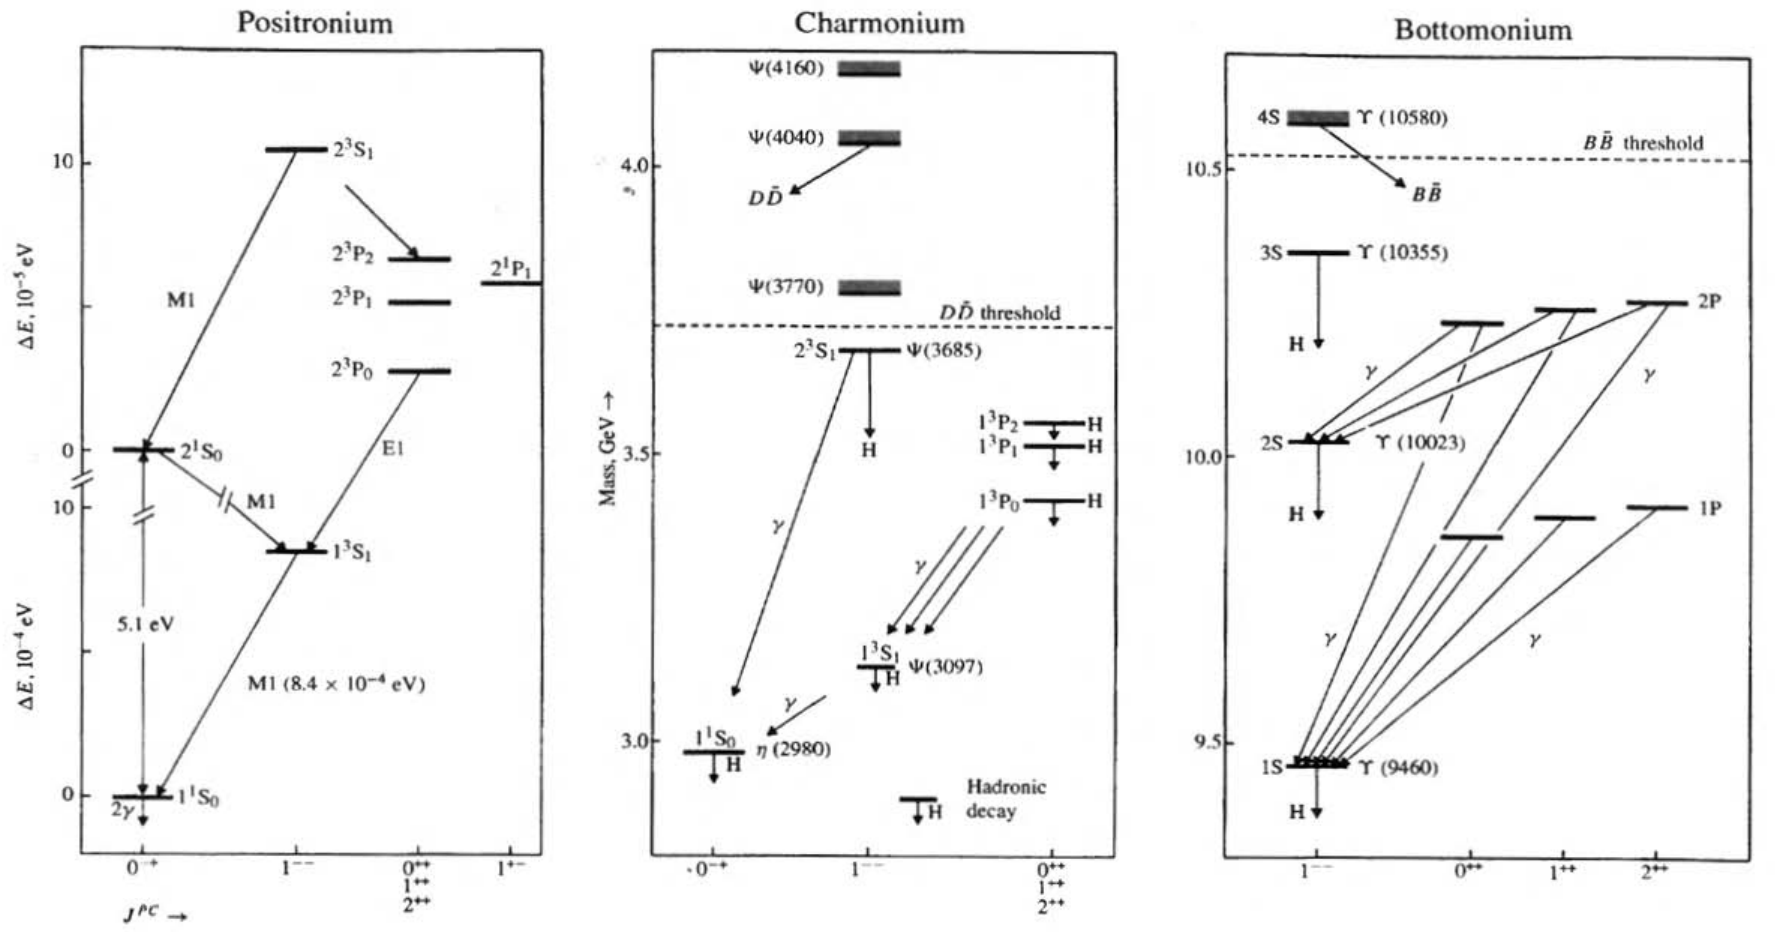
\includegraphics[width=1\linewidth]{Imagenes/NivelesEnergiaEECCBB.png}
    \caption{Niveles de energía del positrionio, charmonio ($c\bar{c}$) y bottomonio ($b\bar{b}$). }
    \label{fig:espectros eeccbb}
\end{figure}
La energía y la masa del charmonio $(c\bar{c})$ vienen dadas por 
$$E_n^{(c\bar{c})}=-\frac{1}{2}\mu c^2 \frac{\alpha_s^2}{n^2} \ \text{con} \ \mu=\frac{m_c}{2} \Rightarrow M_{c\bar{c}}=2mcc^2+E_n^{c\bar{c}}=2m_cc^2 \qty(1-\frac{\alpha_s^2}{8n^2})$$
Si comparamos con los datos experimentales y utilizamos la masa de la tabla \ref{tab: Particulas elementales} obtenemos que para el estado fundamental la masa debe ser $M_{c\bar{c}}\sim \unit[2.6]{MeV}$, que se desvía mucho de los datos experimentales.
\begin{table}[h]
\centering
\begin{tabular}{cc|c|c|}
\cline{3-4}
                                             &  & \textbf{$c\bar{c}$} & \textbf{$b\bar{b}$} \\ \hline
\multicolumn{1}{|c|}{\multirow{2}{*}{$n=1$}} & $^1S_0$   & 2984                & 9399                \\ \cline{2-4} 
\multicolumn{1}{|c|}{}                       & $^3S_1$   & 3097                & 9460                \\ \hline
\multicolumn{1}{|c|}{\multirow{6}{*}{$n=2$}} & $^3P_0$   & 3415                & 9860                \\ \cline{2-4} 
\multicolumn{1}{|c|}{}                       & $^3P_1$   & 3511                & 9892                \\ \cline{2-4} 
\multicolumn{1}{|c|}{}                       & $^3P_2$   & 3556                & 9913                \\ \cline{2-4} 
\multicolumn{1}{|c|}{}                       & $^1P_1$   & 3525                & 9899                \\ \cline{2-4} 
\multicolumn{1}{|c|}{}                       & $^1S_0$   & 3638                & 9999                \\ \cline{2-4} 
\multicolumn{1}{|c|}{}                       & $^3S_1$   & 3686                & 10023               \\ \hline
\multicolumn{1}{|c|}{$n=3$}                  & $^3S_1$   & 4040                & 10355               \\ \hline
\multicolumn{1}{|c|}{$n=4$}                  & $^3S_1$   & 4415                & 10580               \\ \hline
\end{tabular}
\caption{Datos experimentales de las masas de los estados de charmonio y bottomonio}
\label{tab: charmonio y bottomonio datos experimentales}
\end{table}

Debemos utilizar  $\alpha_s^2=1.623$ y la \textbf{masa constituyente} de los quarks $c/\bar{c}$, $m_cc^2=\unit[1942]{MeV}$, esta masa es análoga a la masa efectiva en física del estado sólido y representa la influencia de la interacción entre los quaks en el estado ligado.\\\\
Sabemos que el potencial de la interacción fuerte debe incluir un término de confinamiento ya que los quarks no existen libres en la naturaleza, ésto se comprueba al intentar separar los quarks que forman un mesón. Si los intentamos separar alcanzaremos energías que permitan crear una pareja quark-antiquark y se formarán más mesones. A este fenómeno se le conoce como \textbf{confinamiento} y nos sugiere que el potencial de la interacción fuerte debe tener un término adicional.
\\\\
Si intentamos ajustar este término con los potenciales más usuales, pozo infinito cuadrado, oscilador armónico, potencial lineal... El que reproduce mejor las medidas experimentales es el potencial lineal.
\begin{equation*}
    V_\mathrm{c}(x)=\left \{  \begin{aligned}
        &\Lambda^2 x \ \text{si} \ x\ge0 \\
        & 0 \ \text{si} \ x<0
    \end{aligned}\right.
\end{equation*}
Si resolvemos la ecuación de Schrödinger con dicho potencial, la solución es analítica y se conoce como funciones de Airy ($\mathrm{Ai}(x)$), así la ecuación de ondas será
\begin{equation*}
    \Psi_n(x)=N\qty(2m\hbar \Lambda^2)^{1/3} \mathrm{Ai}\qty(\qty(2m\hbar \Lambda^2)^{1/3}+\qty(x-\frac{E_n}{\Lambda^2})\frac{1}{\hbar})
\end{equation*}
Si imponemos que la función de onda ha de anularse en el orígen, es decir $\Psi_n(0)=0$, encontramos que $$E_n=\frac{\Lambda^2\hbar}{\qty(2m\hbar \Lambda^2)^{1/3}}(-\xi_n)$$ Donde $\xi_n$ son los ceros de las funciones de Airy.
\\\\
Es decir, que el potencial de la interacción fuerte a distancias cortas tiene un comportamiento del tipo coulombiano mientras que a largas distancias entra el juego el confinamiento y se comporta como un potencial lineal, al potencial que se comporta de esta manera se le conoce como \textbf{potencial de Cornell}
\begin{equation}
    V(r)=-\frac{k}{r}+\frac{r}{a^2}
\end{equation}
Este potencial no tiene solución analítica pero si introducimos la interacción spin-spin en teoría de perturbaciones reproducimos el espectro de energía de los mesones pesados de manera bastante precisa\footnote{Se puede completar más el espectro añadiendo términos de aniquilación.}. 

\section{Propiedades fundamentales de la interacción débil}
La interacción débil tiene un problema fundamental y es que \textbf{no} forma estados ligados. Por lo tanto debemos estudiarla a partir de reacciones.\\\\ Sólo se da en aquellos casos en los que las interacciones fuerte y electromagnética estén prohibidas. En consecuencia los procesos débiles tienen \textbf{vidas medias muy largas}, generando un espectro muy amplio ya que tenemos ejemplos como el neutrón con $\tau_n \sim \unit[10^3]{s}$ y el pión con $\tau_\pi \sim \unit[10^{-8}]{s}$ debido a que la diferencia de energías entre el estado final e inicial es muy pequeña (explicación en la sección \ref{sec: particulas virtuales}).
\newpage
\noindent
\begin{minipage}{0.5\linewidth}
    La interacción débil conserva:
\begin{itemize}
    \item Momento angular, $J$ y carga $Q$.
    \item Números leptónicos de cada familia, $L_i$.
    \item Número bariónico, $B$.
\end{itemize}
\end{minipage}
\hfill
\begin{minipage}{0.4\linewidth}
    La interacción débil no conserva:
    \begin{itemize}
        \item Paridad y $C-$paridad.
        \item Isospín y número de quarks.
        \item Sabor.
    \end{itemize}
\end{minipage}\\\\

Y viene mediada por 3 bosones gauge: $W^\pm, Z^0$. Hasta 1973, se entendían todos los procesos sólo con $W^\pm$ pero el Modelo Standar exigía la existencia del $Z^0$ que se descubrió a finales de los 70. Así podemos clasificar los procesos débiles en \textbf{corrientes cargadas}, mediadas por $W^\pm$; y \textbf{correntes neutras}, mediadas por $Z^0$.\\\\
Otra clasificación que podemos hacer es en función de las partículas que participan en las reacciones y que son
\begin{itemize}
    \item \textbf{Leptónicos}: Si \textbf{todas las partículas} son leptones. Por ejemplo: $\mu^- \longrightarrow e^- +\nu_\mu + \overline{\nu}_e$.
    \item \textbf{Semileptónicos}: Si involucra hadrones y leptones. Por ejemplo: $n \longrightarrow p+ e^-  + \overline{\nu}_e$
    \item \textbf{Hadrónicos}: Si \textbf{todas las partículas} son hadrones. Por ejemplo: $\Lambda \longrightarrow p +\pi^-$
\end{itemize}
\subsection{Corrientes cargadas. Procesos Leptónicos}
\noindent
\begin{minipage}{0.6\textwidth}
    En los procesos leptónicos el bosón débil se ``lleva'' la carga del leptón cargado, transformándolo en su correspondiente neutrino, y se la transfiere a un leptón más ligero, generando además el antineutrino correspondiente.\\\\
    Cada vértice del diagrama \ref{fig: desintegracion muon} es leptónico, por lo que tienen la misma carga $g_W$. Por lo tanto la probabilidad que tiene de darse este proceso es $P\sim \abs{\alpha_W}^2$ con $\alpha_W=\dfrac{\alpha}{m_W}$ y $\alpha \sim g^2$.
\end{minipage}
\hfill
\begin{minipage}{0.35\textwidth}
    \centering
    \includegraphics[width=0.8\textwidth]{Diagramas Tema 2/DesintegracionMuonII.pdf}
    \captionof{figure}{Desintegración débil del muón.}
    \label{fig: desintegracion muon}
\end{minipage}
\subsection{Corrientes cargadas. Procesos semileptónicos}
En estos procesos encontramos tanto quarks como leptones. Si intentamos medir cómo se acopla el mesón $W^-$ a los quarks tenemos un problema, pues los quarks tienen color y no seríamos capaces de ver la reacción fundamental. Para estudiar estos procesos se hicieron dos hipótesis
\newpage
\subsubsection{Simetría quark-leptón}
\noindent
\begin{minipage}{0.6\textwidth}
    Los leptones y los quarks los tenemos agrupados en 3 familias. Puesto que todas las partículas participan en la interacción débil, se postuló que los quarks de la 1ª familia $(u,d)$ participan de la misma manera que los leptones de la 1ª familia $(e^-,\nu_e)$.\\\\
Cuando se introdujo esta simetría, no se conocía el quark $c$. Pero ahora podemos generalizarlo también a la 2ª familia, así
\begin{equation}
    \mqty(u\\d) \Leftrightarrow \mqty(e^-\\\nu_e), \quad \mqty(c\\s) \Leftrightarrow \mqty(\mu^-\\\nu_\mu) 
\end{equation}
En la sección \ref{sec: universalidad de la interaccion debil}, demostramos que las diferentes familias de leptones participaban de igual manera en la interacción débil. Por lo tanto si asociamos $g_W$ a $W^\pm$, como ya hicimos en los procesos leptónicos, esa $g_W$ será la misma para todos los leptones, lo que significa que $g_W=g_{ud}=g_{cs}$.
\end{minipage}
\hfill
\begin{minipage}{0.35\textwidth}
    \centering
    \includegraphics[width=\textwidth]{Diagramas Tema 2/DiagramadeQuarksBeta-.pdf}
    \captionof{figure}{Diagrama de Feynmann de la desintegración $\beta^-$.} \label{fig: desintegracion beta}
    \vspace{1.5cm}
    \includegraphics[width=\textwidth]{Diagramas Tema 2/DesintegracionPion+.pdf}
    \captionof{figure}{Diagrama de Feynmann de la desintegración del $\pi^-$.} \label{fig: desintegracion pion}
\end{minipage}\\\\

\noindent Por ello, como el $W^\pm $ mezclaba leptones de la misma familia, también lo hará con quarks de la misma familia. Fue así como se pudo entender los procesos \ref{fig: desintegracion beta} y \ref{fig: desintegracion pion}.
\subsubsection{Mezcla de quarks. Postulado de Cabibbo}
Aunque se entendían muchos de los procesos debido a la simetría quark-leptón, había un proceso que no se entendía ya que mezcla distintas familias de quarks.
$$K^-(s\bar{u})\longrightarrow \mu^-+\bar{\nu}_\mu$$

Cabibbo definió un estado $d^\prime$ que es combinación del quark $d$ y $s$. Así la 1ª familia de quarks está formada por $\mqty(u\\d^\prime)$. Este nuevo estado se define como 
\begin{equation}
d^\prime=d\cos(\theta_\mathrm{C})+s\sin(\theta_\mathrm{C})
\label{eq: estado mezcla ds}
\end{equation}
Así podemos tener vértices que mezclan $(u,d)$ y $(u,s)$ (Figura \ref{fig:vertices UD}), modificando así el valor de las constantes de interacción de esos vértices.
\begin{equation}
    \begin{aligned}
        &g_{ud}=g_W \cos{(\theta_\mathrm{C})}\\
        &g_{us}=g_W \sin{(\theta_\mathrm{C})}
    \end{aligned}
    \label{eq: constantes mezcla}
\end{equation}
\begin{figure}[h]
    \centering
    \includegraphics[width=0.5\linewidth]{Diagramas Tema 2/VerticesUD.pdf}
    \caption{Vértice ($ud^\prime W$) y su interpretación como suma de vértices ($udW$) y ($usW$). El vértice $(usW)$ está suprimido por el ángulo de Cabibbo.}
    \label{fig:vertices UD}
\end{figure}
Ahora bien, tenemos que tener en cuenta que el ángulo de Cabibbo $(\theta_\mathrm{C})$, debe ser pequeño para no modificar lo que conocemos sobre la desintegración del pión y que esté suprimido para el kaón
\newpage
Tras la propuesta de la existencia del quark $c$ por parte de Glashow, Iliopoulos y Maiani (GIM) en 1970, se modificó la teoría de Gell-Mann de la existencia de un doblete y un singlete a dos dobletes y en analogía al quark $d$, se introdujo un estado $s^\prime$ ortogonal al estado $d^\prime$
\begin{equation}
    s^\prime=-d\sin(\theta_\mathrm{C})+s\cos(\theta_\mathrm{C}) 
    \label{eq: estado mezcla sd}
\end{equation}

La introducción del quark encantado permite introducir una matriz para pasar de los quarks físicos a los quarks descritos por la teoría débil a través de 
\begin{equation}
   Q= \mqty(-\sin(\theta_\mathrm{C}) & \cos(\theta_\mathrm{C})\\
    \cos(\theta_\mathrm{C}) &\sin(\theta_\mathrm{C}))
    \label{eq: matriz ckm}
\end{equation}
que se conoce como matriz de intercambio de quarks. Además introduce un nuevo número cuántico \textbf{el encanto}.
Así las constante de interacción \ref{eq: constantes mezcla} serán
\begin{equation}
    \begin{aligned}
        &g_{ud}=g_{cs}=g_W \cos{(\theta_\mathrm{C})}\\
        &g_{us}=-g_{cd}=g_W \sin{(\theta_\mathrm{C})}
    \end{aligned}
    \label{eq: constantes mezcla total}
\end{equation}
Y a los vértices descritos en la figura \ref{fig:vertices UD} tenemos que añadir también los producidos por la desintegración del $c\xrightarrow[]{} s^\prime+W^+$
\begin{figure}[h]
    \centering
    \includegraphics[width=0.5\linewidth]{Diagramas Tema 2/VerticesDS.pdf}
    \caption{Vértice ($cs^\prime W$) y su interpretación como suma de vértices ($cdW$) y ($csW$). El vértice $(cdW)$ está suprimido por el ángulo de Cabibbo debido a la expresión \ref{eq: estado mezcla sd}.}
    \label{fig:vertices DS}
\end{figure}

Ahora queremos determinar el ángulo de Cabibbo, para ello vamos a comparar la desintegración del kaón y la desintegración del pión y la del neutrón y el muón.
\begin{equation}
  \left.  \begin{aligned}
        &\frac{\Gamma\qty(K^-\xrightarrow{}\mu^-+\bar{\nu}_\mu)}{\Gamma\qty(\pi^-\xrightarrow{}\mu^-+\bar{\nu}_\mu)} \sim \frac{g_{us}^2}{g_{ud}^2} \sim \tan^2(\theta_\mathrm{C})\\\\
        &\frac{\Gamma\qty(n\xrightarrow{}p+e^-+\bar{\nu}_e)}{\Gamma\qty(\mu^-\xrightarrow{}e^-+\bar{\nu}_e+{\nu}_\mu)} \sim \frac{g_{ud}^2}{g_{W}^2} \sim \cos^2(\theta_\mathrm{C})
    \end{aligned} \right \} \Rightarrow \theta_\mathrm{C}=13^{\degree}
\end{equation}

\noindent De la comparación de estas dos reacciones tenemos que $\dfrac{g_{us}^2}{g_{ud}^2}=\dfrac{g_{cd}^2}{g_{cs}^2}=\tan^2(\theta_{C})$, con lo que todos los procesos débiles que contengan un quark $c$ en el estado final estarán favorecidos a tener un quark $s$ en el estado final. Esto hace que todo aquello que vaya medido por $g_{us}$ y $g_{cd}$ son procesos suprimidos por Cabibbo; y los medidos por $g_{ud}$ y $g_{cs}$ están favorecidos. \\\\
Así tenemos que los decaimientos del quark $c$ en quarks ligeros por el ángulo de Cabibbo son
\begin{equation}
    \begin{aligned}
        &c\longrightarrow s+l^++\nu_l \quad \text{con} \quad l=e,\mu\\
        & c\longrightarrow s+u+\bar{d}
    \end{aligned}
    \label{eq: Decaimientos favorecidos c}
\end{equation}

\subsubsection{Reglas de selección}
De la teoría de Cabibbo podemos extraer reglas de selección para no tener necesidad de dibujar el diagrama de quarks.\\\\
Para estudiar la regla de selección en procesos semileptónicos estudiemos los siguientes procesos
\begin{equation*}
    \begin{aligned}
        &\Sigma^- \longrightarrow n+e^-+\bar{\nu}_e \\
        &\Sigma^+ \longrightarrow n+e^++\nu_e
    \end{aligned}
\end{equation*}
Si comparamos los espacios fásicos son exactamente iguales por lo que podríamos suponer que $R_\mathrm{th}=\dfrac{\Gamma\qty(\Sigma^+ \longrightarrow n+e^++\nu_e)}{\Gamma\qty(\Sigma^- \longrightarrow n+e^-+\bar{\nu}_e)}\simeq 1$ pero experimentalmente hemos sabemos que $R_\mathrm{exp}<5\cdot 10^{-3}$. \\\\
Debemos tener en cuenta supresión de Cabibbo, para ello estudiamos la parte hadrónica de ambos procesos
\begin{equation*}
    \begin{aligned}
        &\mathrm{Proceso} \ \Sigma^- : \quad dds \longrightarrow ddu \\
        &\mathrm{Proceso} \ \Sigma^+:  \quad uus \longrightarrow udd
    \end{aligned}
\end{equation*}

Por lo tanto en el proceso $\Sigma^-$ tenemos que cambiar un quark $s$ por un quark $u$ mientras que en el proceso $\Sigma^+$ tenemos que cambiar dos quarks $u\leftrightarrow d$ y $s \leftrightarrow d$, es decir, tenemos dos cambios de sabor (dos emisiones de un bosón $W$), lo cual la probabilidad de este proceso es despreciable ($P\sim \abs{\alpha_W}^4$).\\\\
Vamos a analizar procesos que sólo\footnote{Nos centramos en la parte hadrónica, a los leptones no afecta a este análisis.} incluyan quarks ligeros y extraños, en estos procesos tenemos dos casos
\begin{itemize}
    \item \textbf{No aparecen quarks extraños}: El intercambio $u\leftrightarrow d$ por lo tanto $\Delta Q=\pm 1$ y $\Delta s=0$.
    \item \textbf{Presencia de quarks extraños}: En estos procesos tenemos la siguiente transformación $$\left \{ \begin{aligned}
        &u\xrightarrow{} s+W^+ \Rightarrow \Delta s =-1=\Delta Q\\
        &s\xrightarrow{} u+W^- \Rightarrow \Delta s =+1=\Delta Q
    \end{aligned} \right.$$
    Por lo que la regla de selección es $\Delta s=\Delta Q=\pm 1$. 
\end{itemize}

Esto garantiza procesos a primer orden, que para el proceso $\Sigma^-, \Delta Q=\Delta s=1$ mientras que para el proceso $\Sigma^+, \Delta Q=-1, \Delta s=+1$ por lo que está \textbf{suprimido} a primer orden.\\\\
Ahora vamos a calcular las reglas de selección para procesos que incluyen encanto. Para ello utilizamos los decaimientos \ref{eq: Decaimientos favorecidos c}, para ello estudiamos las desintegraciones del mesón $D^+(c\bar{d})$:
\begin{equation*}
    \begin{aligned}
        &(1): \quad D^+ \longrightarrow K^-+\pi^++e^++\nu_e \\
        &(2): \quad D^+ \longrightarrow \pi^-+\pi^++e^++\nu_e
    \end{aligned}
\end{equation*}
Como hicimos para los procesos con extrañeza analizamos la parte hadrónica de ambos procesos
\begin{equation*}
    \begin{aligned}
        &\text{Proceso} \ (1): c\bar{d}\xrightarrow[]{} \bar{u}s+u\bar{d}\\
        &\text{Proceso} \ (2):c\bar{d}\xrightarrow[]{} \bar{u}d+u\bar{d}
    \end{aligned}
\end{equation*}

En el proceso (1) los incrementos de sabor y carga son $\Delta c=-1,\Delta s=-1, \Delta Q=-1$. En el proceso (2) los incrementos de sabor y carga son $\Delta c=-1,\Delta s=0, \Delta Q=-1$. Ahora si tenemos en cuenta que los decaimientos favorecidos \ref{eq: Decaimientos favorecidos c} son los que tienen incremento de extrañeza, por lo tanto $\Delta c=-1, \Delta s=-1, \Delta Q=-1,0$ \footnote{Quitamos la contribución de $\Delta Q=0$ ya que en corrientes neutras los cambios de sabor están suprimidos (página siguiente).}. Por lo tanto $\boxed{\Delta s=\Delta c=\Delta Q=\pm 1}$.
\subsection{Corrientes cargadas. Procesos hadrónicos}
Estos procesos están descritos por simetría Quark-Leptón + Mezcla de Quarks. Estos procesos sólo tienen hadrones en ambos lados de la reacción como vimos en la figura \ref{fig: diagrama de quarks delta ++ posible}.
\subsubsection{Reglas de selección. Incremento de extrañeza}
En estos procesos necesariamente la carga se tiene que conservar, por lo tanto $\Delta Q=0$ y sólo tenemos cambios en la extrañeza $\Delta s=0,\pm1$.\\\\
Vamos a suponer que el barión cascada $\Xi^- (ssd)$ se puede desintegrar por los siguientes canales:
\begin{equation*}
    \begin{aligned}
        &\quad \Xi^- \longrightarrow \Lambda^0+\pi^- \ \Delta Q=0 \ \Delta s=+1 \\
        &\quad \Xi^- \longrightarrow n+\pi^- \ \Delta Q=0 \ \Delta s=+2
    \end{aligned}
\end{equation*}
En la naturaleza sólo se observa el primer proceso, pues el segundo necesita de al menos dos bosones $W$. Análogamente para la partícula $\Omega^-$ tenemos la siguiente cadena
$$\Omega^-\xrightarrow[]{} \textcolor{red}{\Xi^0}+\pi^- \xrightarrow[]{} \textcolor{red}{\Lambda^0}+\pi^0 \xrightarrow[]{} \textcolor{red}{p+\pi^-}$$

\noindent Cada una de los diferentes pasos tienen un cambio de extrañeza $\Delta s=+1$.
\subsubsection{Reglas de selección. Incremento de isospín}

Como ya sabemos el isospín no es una simetría de la interacción débil, dentro de los procesos hadrónicos hay observaciones fenomenológicas acerca de la preferencia de isospín en la naturaleza. Esta violación de isospín la naturaleza va a hacerla en la menor cantidad posible, por lo que la regla de selección es 
\begin{equation}
    \boxed{\Delta s=1, \ \abs{\Delta I}=\frac{1}{2}}
\end{equation}

\noindent Esto se entiende debido a que el cambio $[s (I=0)\leftrightarrow u,d(I=\nicefrac{1}{2})]$.
%Aqui no se si hacer el ejemplo con el teorema de Wigner-Eckart y explicarlo con los apuntes de Eliecer.

\subsection{Corrientes neutras}
Estas corrientes vienen mediadas por el intercambio de bosones $Z^0$. Como necesariamente se tienen que conservar los números leptónicos y la carga, sólo tenemos dos vías por las que se pueden dar las corrientes neutras
\begin{figure}[h]
    \centering
    \includegraphics[width=0.5\linewidth]{Diagramas Tema 2/VerticesNeutros.pdf}
    \caption{Vertices neutros.}
    \label{fig:Vertices neutros}
\end{figure}

Para que en las corrientes neutras podamos tener hadrones necesitamos introducir de nuevo \textbf{simetría quark-laptón + mezcla de quarks}. \\\\ Podemos tener 6 vértices neutros (quarks de la 3ª familia) no suprimidos: $$\nu_e\nu_e Z^0 \quad \nu_\mu\nu_\mu Z^0 \quad e^-e^- Z^0 \quad \mu^-\mu^- Z^0 \quad uu Z^0 \quad d^\prime d^\prime Z^0$$

Fijémonos que estos vértices no tienen intercambio de sabor ya que son los suprimidos, demostrémolos:
\begin{equation*}
    \begin{aligned}
    & d^\prime d^\prime Z^0=ddZ^0 \cos^2\theta_\mathrm{C}+ssZ^0 \sin^2\theta_\mathrm{C} +(dsZ^0+sdZ^0\cos\theta_\mathrm{C})\sin\theta_\mathrm{C}\cos\theta_\mathrm{C}\\
    & s^\prime s^\prime Z^0=ddZ^0 \cos^2\theta_\mathrm{C}+ssZ^0 \sin^2\theta_\mathrm{C} -(dsZ^0+sdZ^0\cos\theta_\mathrm{C})\sin\theta_\mathrm{C}\cos\theta_\mathrm{C}
    \end{aligned}
\end{equation*}

\noindent Que si sumamos ambos vértices vemos que los intercambios de sabor de quarks se suprimen.\\\\
Por lo tanto, los vértices neutros de quarks conservan extrañeza y encanto, al contrario que los vértices de las corrientes cargadas.
Esto se puede comprobar experimentalmente a partir de los decaimientos de los kaones.
\begin{equation*}
    \begin{aligned}
        &K^+\longrightarrow \pi^0 +\mu^++\nu_\mu \quad BR_i=3.35 \cdot 10^{-2} \quad \text{Corriente cargada}\\
        &K^+\longrightarrow \pi^+ +\nu_l+\bar{\nu}_l \ \quad BR_i<1.14\cdot 10^{-10} \quad \text{Corriente neutra}
    \end{aligned}
\end{equation*}

\noindent Si estudiamos las anchuras de desintegración de todos estos procesos $$R_\mathrm{exp}=\frac{\sum_l \Gamma\qty(K^+\xrightarrow[]{} \pi^++\nu_l+\bar{\nu}_l)}{\Gamma\qty(K^+\xrightarrow[]{} \pi^0+\mu^++\nu_\mu )}<10^{-7}$$

Por lo que el proceso neutro está suprimido debido al cambio de extrañeza.
\subsection{Violación de paridad}
La no universalidad de la paridad en los procesos físicos fue una cuestión que trajo muchos dolores de cabeza hasta 1956. En los años 50 había un problema en la física de partículas llamado ``puzzle de la partícula $\tau-\theta\,$'' donde se conocía $\tau \xrightarrow[]{} 2\pi$ y $\theta \xrightarrow[]{} 3\pi$. Hasta que la $\theta$ se midió un modo de desintegración $\theta\xrightarrow[]{} \pi^++\pi^0$. Como los piones tienen $J^P=0^-$, por lo que si imponemos conservación de momento angular tenemos ${J}_\theta={L}_{\pi \pi}$ si imponemos conservación de paridad, el acoplo de momentos angulares debe ser en onda S para paridad + y en onda P para paridad -, por lo que obtenemos la siguiente serie 
$J^P_\theta=0^+,1^-+2^+...$ \\\\
En el caso de la $\tau$ se había medido un modo cargado $\tau^+\xrightarrow[]{} 2\pi^++ \pi^-$ en el que $J^P_\tau=0^-$, por lo que los momentos angulares relativos debían ser iguales.\\\\
Experimentalmente se demostró que estas partícula tenían spin nulo y la misma masa por lo que necesariamente debían ser la \textbf{misma partícula}. Esto supone un problema ya que debemos tener una paridad distinta para una misma partícula.
\subsubsection{Hipótesis de Lee y Yang}

Lee y Yang supusieron que la paridad no se conservaba estrictamente, para decir que $\theta$ y $\tau$ son dos modos de decaimiento de la misma partícula. Esto se puede suponer como una evidencia de que la paridad no se conserva en la interacción débil.
\\\\
Esto trae consigo otro problema, no se conserva con la C-paridad. El hecho de que las partículas y las antipartículas tuvieran la misma media se demostraba como invarianza bajo transformaciones de C-paridad. Aunque esto también se puede demostrar suponiendo invarianza bajo \textbf{transformaciones de Lorentz} como vimos con la ecuación\ref{eq: Ecuacion de Klein-Gordon}.\\\\
En 1956 Madame Wu demostró que la hipótesis de Lee y Yang era correcta, para ello se midió la interacción débil de los núcleos de cobalto-60, que se desintegra por $\beta^-$. Através de $^{60}\mathrm{Co}\xrightarrow[]{}^{60}\mathrm{Ni}+e^-+\bar{\nu}_e$. En los núcleos es fácil determinar el spin y la paridad, por lo que se planteó medir la distribución angular de los electrones emitidos y así determinando si existe una dirección privilegiada para estos electrones.\\\\
Se podían dar dos situaciones:
\begin{itemize}
    \item Si el proceso fuese invariante bajo paridad, la probabilidad debería ser la misma en las direcciones perpendicular y antiperpendicular al campo magnético \footnotemark. 
    \item Si el proceso no fuese invariante bajo paridad, si que existe una dirección privilegiada
\end{itemize}
\footnotetext{Para determinar el spin necesitamos el campo magnético como en el experimento de Stern-Gerlach}

Lo que se observó fue que se emitían más electrones en la dirección contraria al campo por lo que \textbf{no se conservaba} la paridad.
\part{Física Nuclear}
\pagestyle{fancy}
\fancyhead[R]{Física Nuclear y de Partículas: Tema 3}
\fancyhead[L]{4º Grado en Física}
\chapter{El núcleo atómico. Propiedades Globales}
Los núcleos atómicos son complicados de estudiar. Su característica más general es que están formados por \textbf{nucleones}, ésto nos genera el primer problema y es que \textbf{no} tenemos un nucleón privilegiado sobre el que podamos establecer un origen sobre el que realicemos transformaciones.
\section{Generalidades del núcleo}
El núcleo atómico es un sistema muy complejo (muchas partículas), sobre el que tenemos que considerar las 3 interacciones fundamentales: electromagnética fuerte y débil. Por ser un sistema de muchos cuerpos, los estudios se realizan desde un punto de vista fenomenológico.\\\\
Los núcleos por están compuestos por nucleones $(p,n)$ podemos definir tres números: $A$, número másico; $Z$, número atómico; $N=A-Z$, número de neutrones. Podemos establecer así diferentes relaciones entre núcleos:\\\\
\noindent
\begin{minipage}{0.4\textwidth}
    \begin{itemize}
    \item Si tienen \textbf{misma} $Z$ se conocen como isótopos.
    \item Si tienen \textbf{misma} $N$ se conocen como isótonos.
    \item Si tienen \textbf{misma} $A$ se conocen como isóbaros.
\end{itemize}
\end{minipage}
\hfill
\begin{minipage}{0.55\textwidth}
    \begin{tcolorbox}[colback=amber!20, colframe=amber, title={Notación: Representación de los núcleos}]
    Los núcleos los vamos a representar através de su símbolo químico $X$ y índices, $A$ como superíndice y $Z$ como subíndice a la izquierda, a veces representaremos $N$ como un subíndice a la derecha.
    \begin{equation}
        ^A_ZX_N
    \end{equation}
\end{tcolorbox}
\end{minipage}\\\\

Se conocen nucleos con número másico $A=1,290$ y unos 2000 núcleos distintos de los quales $\sim250$ son estables y $\sim350$ quasi-estables.

\subsubsection{Estabilidad nuclear}
Otra clasificación que podemos hacer es en función del número de partículas que componen el núcleo, si nos centramos en los núcleos estables encontramos
\newpage

\begin{table}[h]
\centering
\begin{tabular}{c|ccc|}
\cline{2-4}
 & \multicolumn{1}{c|}{Z} & \multicolumn{1}{c|}{N} & \begin{tabular}[c]{@{}c@{}}nº de núcleos \\ estables\end{tabular} \\ \hline
\multicolumn{1}{|c|}{\multirow{2}{*}{A=impar}} & Impar & Par   & $50$  \\
\multicolumn{1}{|c|}{}                         & Par   & Impar & $55$  \\ \cline{1-1}
\multicolumn{1}{|c|}{\multirow{2}{*}{A=par}}   & Par   & Par   & $165$ \\
\multicolumn{1}{|c|}{}                         & Impar & Impar & $4$   \\ \hline
\end{tabular}
\caption{Número de núcleos estables en función del número de nucleones que lo componen. Los núlceos pares tipo $(I,I)$  sólo son 4 y son núcleos ligeros: $^2_1 \mathrm{H},\  ^6_3 \mathrm{Li}, \ ^{10}_5 \mathrm{B}, \  ^{14}_7 \mathrm{N}$.}
\label{tab: nucleos estables en funcion del numero de nucleones}
\end{table}

Si recordamos la figura \ref{fig: Diagrama Segre}, para $A<40, Z\approx N$ tenemos que los núcleos son simétricos, mientras que a partir de $A\sim 40$, el cociente $N/Z$ va aumentando hasta tomar valores de 1.54 (uránidos).\\\\
Existen valores de $Z$ y $N$ denominados \textbf{números mágicos} para los que hay un elevado número de núcleos estables : 2, 8, 20, 28, 50, 82, 126. A partir de $Z>83$ no tenemos núcleos estables ya que se desintegran por emisión de partículas $\alpha$ (núcleos de $^4\mathrm{He}$), el núcleo estable de mayor $Z$ es el $^{209}_{\ 83}\mathrm{Bi}$.\\\\
Los núcleos atómicos pueden tener en lugar de un nucleón un barión $\Delta$, lo que se conoce como \textbf{hipernúcleos}, así tenemos isótopos como el $^{\ \ 6}_{\Lambda \Lambda}\mathrm{He}$ constituído por $^{\ \ 6}_{\Lambda \Lambda}\mathrm{He}=2p+2n+2\Lambda$, estos núcleos no son estables en la superficie de la Tierra, pero pueden existir en situaciones extremas como cortezas de estrellas de neutrones.

\subsubsection{Sistema de muchas partículas}
Debido a que el núcleo es un sistema de muchas partículas, tenemos un número de grados de libertad demasiado grande como para poder considerarlos todos, por ello utilizaremos un conjunto de observablaes a los que denominamos \textbf{propiedades estáticas del núcleo}: Carga eléctrica, radio nuclear, masa nuclear, energía de ligadura, momento angular, paridad, momentos electromagnéticos...

\section{Distribución de carga y masa nuclear. Factores de forma}

El tamaño y la forma de un objeto se analizan a partir de la radiación que dispersan, para ello necesitamos que la longitud de onda de la radiación \footnote{No tiene que ser necesariamente radiación electromagnética, recordar que existe la longitud Compton\\ $\lambda_\mathrm{C}=\dfrac{h}{p}$}con la que estamos bombardenado el objeto sea $\lambda \lesssim $ tamaño del objeto. Así podemos determinar las distribuciones de carga y masa:
\begin{itemize}
    \item \textbf{Distribución carga nuclear}: se determina mediante un scattering del núcleo con electrones, y permiten determinar la estructura interna (protones y neutrones) del núcleo. La razón por la que se utilizan leptones se debe a que ellos \textbf{no} participan en la interacción fuerte.
    \item \textbf{Distribución de masa nuclear}: se determina a partir de un scattering Rutherford, para ello se utilizan partículas $\alpha=2p+2n$ a muy alta energía, esto hace que podamos romper el scattering Rutherford y entre en juego la fuerza fuerte, lo que nos permite ver el tamaño del núcleo.
\end{itemize}
\subsection{Distribución de carga nuclear}
Si recordamos de la figura \ref{tab: comparacion de escalas}, el radio nuclear es de $r_\mathrm{N}\sim \unit[10]{fm}$, por lo que la longitud de onda que deben tener los electrones con los que bombardeemos el núcleo será $$\lambda \lesssim \unit[10]{fm} \Rightarrow p>\dfrac{h}{\lambda}=\dfrac{2\pi \hbar c}{pc}\sim \unit[100]{MeV/\textit{c}^2}$$

Por lo que estamos utilizando electrones \textbf{ultrarrelativistas} $(pc\gg mc^2)$. Este tratamiento nos permite realizar un tratamiento ondulatorio del electrón, si suponemos que el núcleo es un disco esférico de diámetro $D$, nos aparece como no podía ser de otra manera un patrón de Airy que toma por expresión en el primer mínimo:
\begin{equation}
    \sin\theta=1.22\frac{D}{\lambda}
    \label{Difraccion de Airy}
\end{equation}
    \begin{tcolorbox}[colback=airforceblue!20, colframe=airforceblue, title={Ejemplo: Patrones de difracción del $^{12}\mathrm{C}$ y $^{16}\mathrm{O}$.}]
Si incidimos con un haz de electrones con una energía de $\unit[420]{MeV}$ sobre un núcleo de $^{12}\mathrm{C}$ encontramos que el primer mínimo se encuentra a 51,5\degree, así podemos obtener el tamaño del núcleo $$\lambda=\frac{2\pi \hbar c}{pc}\Rightarrow D=\frac{1.22}{\sin(51.5\degree)} \frac{2\pi 197.327}{420}=\unit[4.6]{fm}$$
Por lo que el radio del $^{12}\mathrm{C}, r(^{12}\mathrm{C})=\unit[2.3]{fm}$, del mismo modo si incidimos con un haz con la misma energía sobre $^{16}\mathrm{O}$ encontramos que el primer mínimo de difracción está en 43.8\degree lo que nos da un radio de $r(^{16}\mathrm{O})=\unit[2.6]{fm}$.\\\\
Así mismo si cambiamos la energía del haz incidente a $\unit[360]{MeV}$ para el oxígeno-16, encontramos el mínimo en $53.9\degree$ que nos da el mismo radio.
\end{tcolorbox}

\noindent \begin{minipage}{0.6\textwidth}
    Si realizamos un scattering sobre núcleos pesados, observamos que hay varios mínimos de difracción a diferentes ángulos pero ninguno se hace nulo (figura \ref{fig:Scattering de electrones y nucleos}), este comportamiento se debe a que el núcleo no es rígido como una bola de billar, sino que es difuso al estilo de la nube electrónica de un átomo (figura \ref{fig: Distribucion de carga nuclear}).\\\\
De la figura \ref{fig: Distribucion de carga nuclear} podemos extraer que la densidad de carga del núcleo es aproximadamente igual en el centro independientemente de $A$. A medida que nos alejamos del centro la densidad de carga empieza a caer de manera progresiva, así definimos \textit{skin thickness} ($t$) como la distancia en la que la densidad de carga pasa de valer el 90\% de su valor central al 10\%.
\end{minipage}
\hfill
\begin{minipage}{0.35\textwidth}
    \centering
    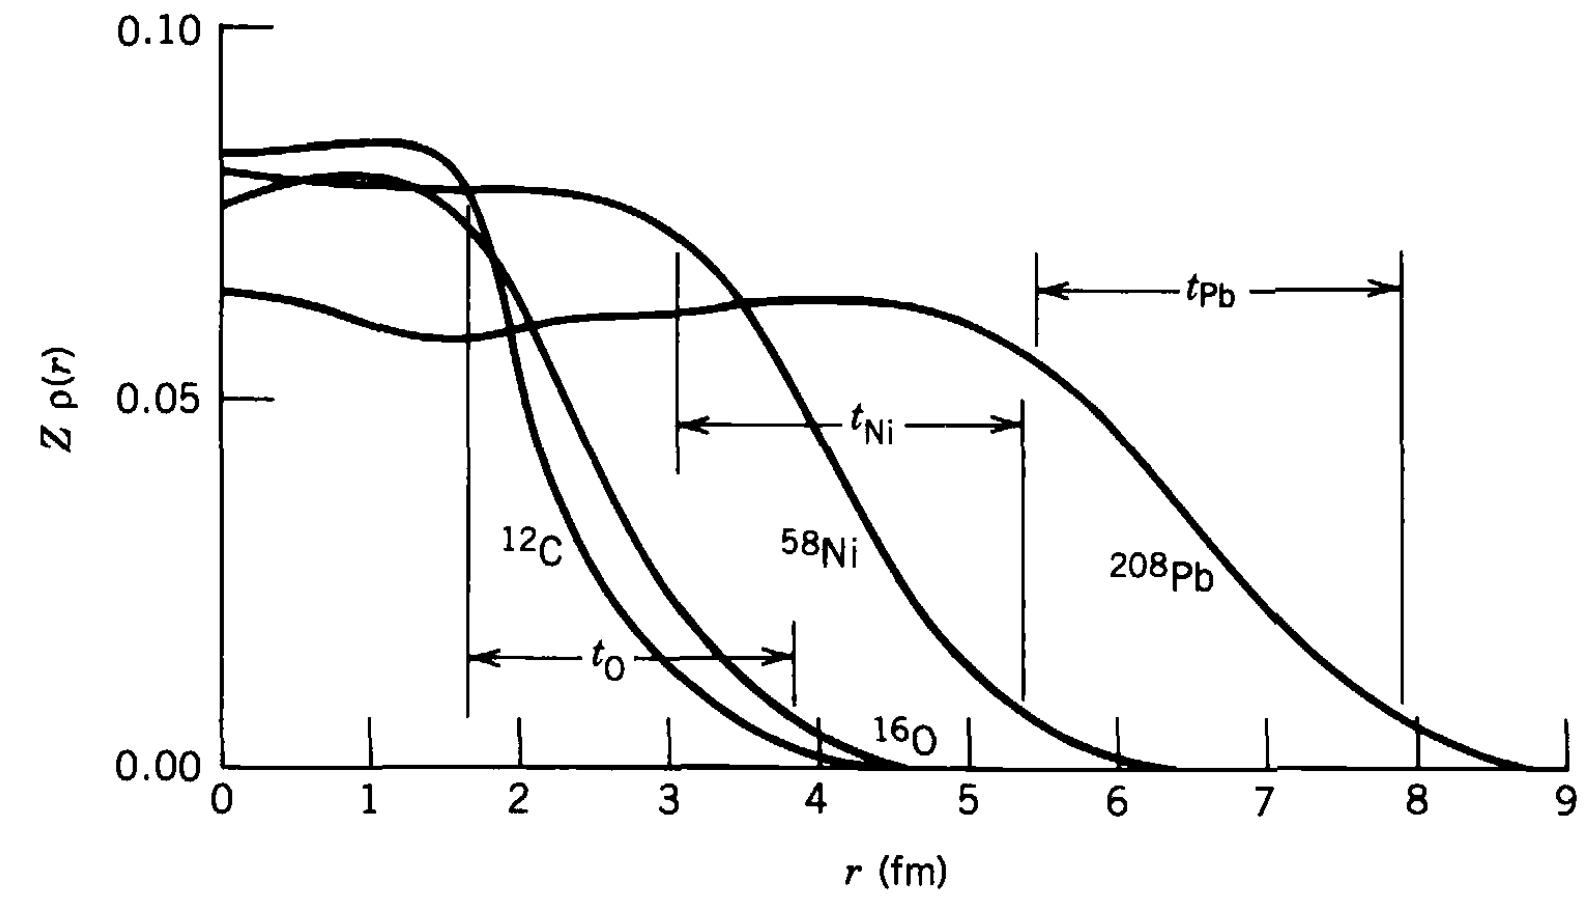
\includegraphics[width=\linewidth]{Diagramas Tema 3/Densidad de carga nucleos.png}
    \captionof{figure}{Distribución de carga de distintos núcleos en función del radio.}
    \label{fig: Distribucion de carga nuclear}    
\end{minipage}

\noindent
\begin{minipage}{0.55\textwidth}
Una cantidad de gran importancia para la física nuclear es la sección eficaz de un scattering elástico de electrones con una carga puntual (scattering $e^-+e^+$). En un scattering relativista tenemos que la sección eficaz diferencial viene dada por 
\begin{equation}
    \eval{\dv{\sigma}{\Omega}}_\mathrm{Mott}=\frac{\alpha^{2}Z^{2}(\hbar c)^{2}}{4E^{2}v^{4}\sin^{4}\left(\frac{\theta}{2}\right)}\left[1-\frac{v^{2}}{c^{2}}\sin^{2}\left(\frac{\theta}{2}\right)\right]
    \label{eq: seccion eficaz mott}
\end{equation}

Que es la versión relativista del scattering Rutherford. Ahora bien, si cambiamos la carga puntual por un núcleo, simplemente tenemos que introducir el \textbf{factor de forma}\footnotemark.
\begin{equation}
    \eval{\dv{\sigma}{\Omega}}_\mathrm{Exp}=\eval{\dv{\sigma}{\Omega}}_\mathrm{Mott}\abs{F(q)}^2
\end{equation}
\end{minipage}
\footnotetext{El desarrollo del factor de forma y del radio cuadrático medio lo encontramos en el apéndice \ref{chap: Apendice C}.}
\hfill
\begin{minipage}{0.4\textwidth}
    \centering
    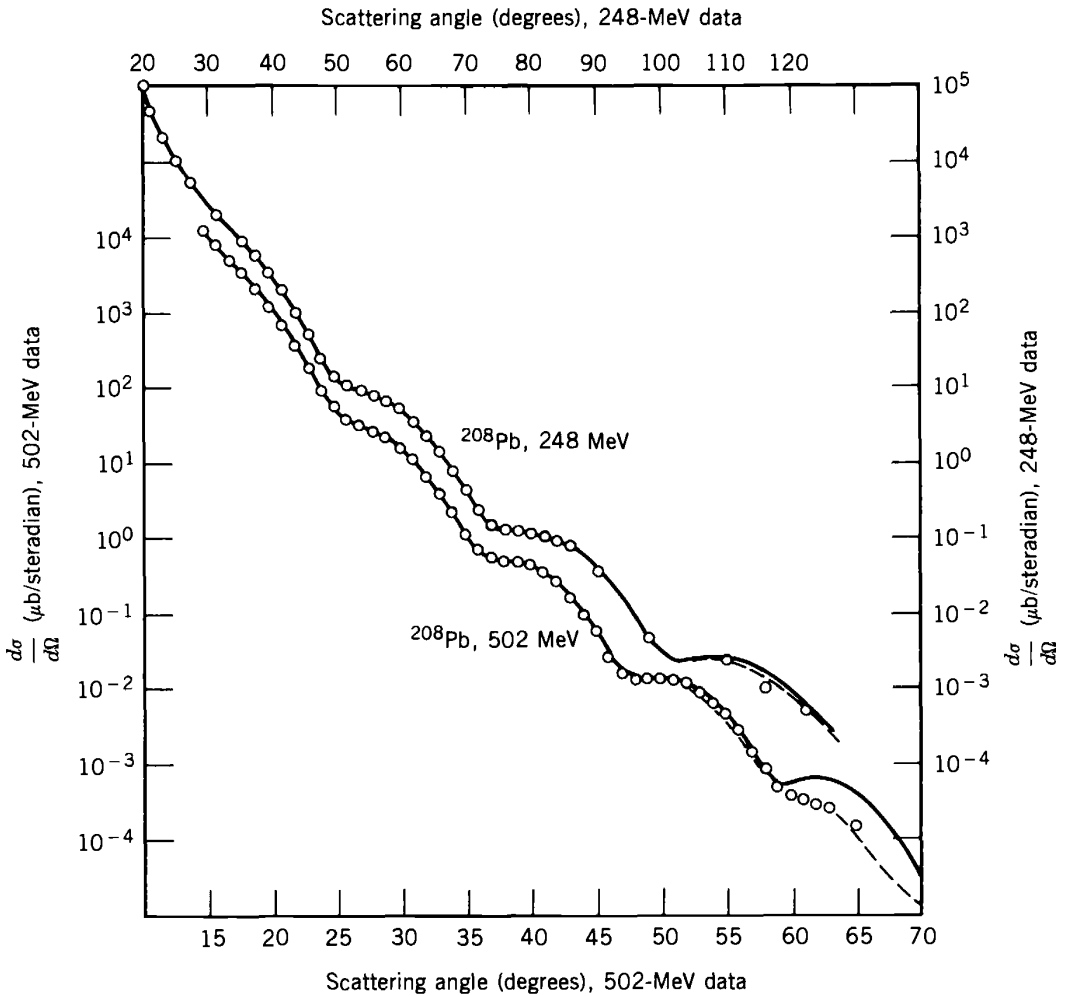
\includegraphics[scale=0.25]{Diagramas Tema 3/Scattering de Plomo.png}
    \captionof{figure}{Scattering de electrones sobre núcleos de $^{208}\mathrm{Pb}$.}
    \label{fig:Scattering de electrones y nucleos}
\end{minipage}
\\\\

Así podemos hacer predicciones postulando la distribución de carga y calculando su factor de forma podemos ver cómo se amolda a los datos experimentales\footnote{El proceso inverso es imposible realizarlo ya que no es posible alcanzar todos los datos numéricos necesarios para realizar al integral impropia de la transformada.}. Volviendo al análisis que hicimos de la figura \ref{fig: Distribucion de carga nuclear} podemos determinar el radio nuclear 
\begin{equation}
 \frac{A}{\frac{4}{3}\pi R^3}=\text{cte} \Rightarrow R=R_0A^{1/3} \quad \text{con} \quad R_0=\unit[1.23]{fm}
    \label{eq: radio nuclear}
\end{equation}

\noindent Mientras que para la \textit{skin thickness} tenemos que el valor es $t\approx \unit[2.3]{fm}$.
\\\\
La distribución que mejor reproduce estos resultados es la distribución de Fermi
\begin{equation}
    \rho(r)=\dfrac{\rho_0}{1+\exp{\dfrac{r-c}{a_0}}}
    \label{eq: distribucion de Fermi}
\end{equation}
Donde $c$ es la disntancia donde $\rho(c)=\dfrac{1}{2} \rho_0$, y $a_0$ es un parámetro empírico que nos dice cómo decae la distribución, que para núcleos con $A\ge 20$ tenemos que 
\begin{equation*}
    c=\unit[1.07 A^{1/3}]{fm} \quad \quad \quad a_0=\unit[0.54]{fm}\equiv \text{cte}
\end{equation*}
\subsubsection{Radio equivalente de una distribución de carga uniforme}
Si calculamos el radio cuadrático $\expval{r^2}=\displaystyle  \dfrac{\int_0^\infty r^4 \rho \dd r}{\int_0^\infty r^2 \rho \dd r}=\dfrac{3}{5}R^2$, así $\expval{r^2}^{1/2}=\sqrt{\frac{3}{5}}R\approx \unit[0.94 A^{1/3}]{fm}$. Obtenemos el radio equivalente de una distribución uniforme, lo que es más fácil de integrar y no se aleja demasiado de los resultados experimentales.
\newpage

\subsubsection{Métodos alternativos}
El análisis de las distribuciones de carga lo podemos hacer a partir de transiciones atómicas, para ello hacemos uso de los potenciales
\begin{equation}
    V_\mathrm{Puntual}(r)=-\frac{Ze^2}{4\pi \varepsilon_0 r} \quad \quad V_\mathrm{Extenso}(r)= \left \{
\begin{aligned}
& \quad\frac{-Ze^2}{4\pi\varepsilon_0R}\left\{\frac{3}{2}-\frac{1}{2}{\left(\frac{r}{R}\right)}^2\right\} \quad \text{si} \quad r\le R \\\\
& \quad\frac{-Ze^2}{4\pi\varepsilon_0r} \quad \text{si} \quad r\ge R
\end{aligned} \right.
\label{eq: potenciales de transicion atomica}
\end{equation}

Si utilizamos que la transiciones más probables son aquellas que siguen la regla de selección $\Delta \ell =1$, tenemos que la función de onda del orbital más interno es $\Psi(r)=\displaystyle \sqrt{\frac{Z^3}{\pi a_0^3}}\exp{-\frac{Zr}{a_0}}$ con lo que la diferencia de energía entre núcleos puntuales y extenso es es 
\begin{equation}
    \Delta E=\expval{V}_\mathrm{Extenso}-\expval{V}_\mathrm{Puntual}=\frac{2}{5} \frac{Z^4e^2}{4\pi\varepsilon_0}\frac{R^2}{a_0^3}
\end{equation}
Para transiciones $K_\alpha (2p \xrightarrow{} 1s)$ encontramos que el incremento de energía en isótopos vecinos es
\begin{equation*}
    E_K(A)-E_K(A^{\prime})=-\frac{2}{5}\frac{Z^4e^2}{4\pi\varepsilon_0}\frac{R_0^2}{a_0^3}{\left(A^{2/3}-{A^{\prime }}^{2/3}\right)}
\end{equation*}

Esto nos permite hacer un ajuste obteniendo que $R_0=\unit[1.2]{fm}$ como no podía ser de otra manera.\\\\
La ventaja de utilizar este método es que nos permite estudiar los núcleos de $Z$ elevado, ya que si cambiamos un electrón por un muón el radio de Bohr $(a_0^\mu(\mathrm{^{208}Pb})=\unit[3]{fm})$ se reduce considerablemente y encontramos que el muón puede estar dentro del núcleo ya que $R=\unit[7.1]{fm}$.
\subsection{Distribución de masa nuclear}
Hasta ahora hemos utilizado únicamente el scattering de leptones con protones, pero queremos saber la relevancia que tienen los neutrones dentro del mismo.\\\\
Como ya hemos mencionado, para estudiar esta distribución utilizamos partículas $\alpha$ y en función de la energía cinética que tengan las partículas podemos determinar la influencia de la interacción fuerte.\\\\
De la misma manera que utilizamos muones para estudiar el núcleo atómico, podemos utilizar piones ya que estos participan en la interacción fuerte. Comparando los rayos X emitidos por un átomo piónico con los calculados usando sólo la interacción coulombiana obtenemos información acerca de la extensión del núcleo. Por último como la absorción de los piones por parte de los nucleones no emite rayos X se genera un defecto que también puede ser medible.
\newpage
\section{Spín, paridad y momentos electromagnéticos nucleares}
Como ya sabemos, el núcleo es un sistema formado por $A$ cuerpos, pero el hamiltoniano que describe este sistema $H= \displaystyle \sum_i^A -\dfrac{\hbar^2}{2m_i} \laplacian-V(\vec{r}_1,\cdots, \vec{r}_A)$ no es posible resolverlo de manera exacta. Sin embargo el simple hecho de que se pueda escribir nos dice que podemos tener estados ligados (espectro discreto de energía), además la función de onda que describa los estados del núcleo debe ser completamente antisimétrica, por último sabemos que los estados excitados se desintegran emitiendo radiación electromagnética.

\subsection{Spín nuclear}

Definimos el momento angular de un núcleo como la suma de los momentos angulares de spin $s_i$ y momentos angulares orbitales $l_i$
\begin{equation}
    \vec{J}=\sum_i^A \vec{l}_i+\vec{s}_i=\sum_i^A \vec{j}_i
\end{equation}

Como le potencial no tiene por qué ser central no podemos utilizar el momento angular orbital como número cuántico pero sí que podemos utilizar el total, tomando los operadores $J_z$ y $J^2$ para la base de autofunciones los valores esperados son $\expval{J_z}=\hbar m$ con $m=-J,\cdots, J$ y $ \expval{J^2}=J\hbar^2(J+1)$.
\\\\
\noindent Tenemos varias restricciones sobre los momentos angulares totales de los nucleones:
\begin{itemize}
    \item Por ser fermiones, los nucleones tienen $j_i$ semientero, por lo que si $A$ es par, $J$ es un entero mientras que si $A$ es impart $J$ es semientero.
    \item Experimentalmente se ha medido que para los nucleos con $(Z,N)=$ (par,par) el estado fundamental es $J=0$. El $J$ de un núcleo con $A$ semientero, se puede entender en muchas ocasiones en términos del spin del nucleón desapareado.
\end{itemize}

\noindent Al hecho de que en el estado fundamental de los núcleos con $A$ par $J=0$ se le conoce como \textbf{pairing}, esto confiere estabilidad a los núcleos ya que los acoplamientos de spin sólo se dan en partículas idénticas, es decir, $(p,p)$ y $(n,n)$ ya que son los únicos casos en los que podemos tener acoplamiento a spin total $J=0,1$.

\subsection{Paridad nuclear}
Como la paridad es una simetría de la interacción fuerte y de la interacción electromagnética, debe ser un buen número cuántico para los estados nucleares. Como vemos en la figura \ref{fig:espectro de energia y JP de los nucleos}, los estados están identificados por $J^P$ y dentro de un núcleo podemos tener distintos estados excitados.
\newpage
\begin{figure}[h]
    \centering
    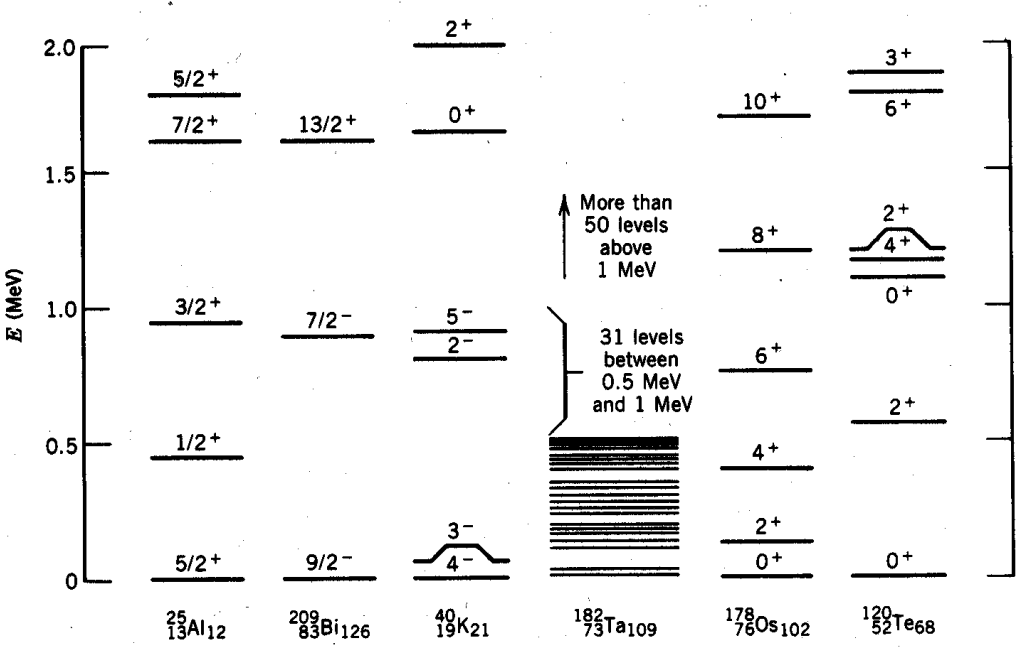
\includegraphics[width=0.7\linewidth]{Diagramas Tema 3/Espectro de energía de distintos nucleos.png}
    \caption{Espectro de energía de diferentes núcleos atómicos. Se muestran además la $J^P$ los diferentes estados de los núcleos.}
    \label{fig:espectro de energia y JP de los nucleos}
\end{figure}

La paridad de los nucleones por convenio está fijada a $P_N =+$ mientras que para los antinucleones será $P_{\Bar{N}} =-$. La paridad del núcleo la podemos calcular entonces como\\ $P=(-)^L\prod_i^A P_i$, pero como no podemos conocer los diferentes momentos angulares orbitales, tomaremos la paridad del nucleón como un dato experimental que \textbf{no} tiene relación teórica con el momento angular total $J$ del núcleo.
\\\\
Experimentalmente se ha medido que para los núcleos (par,par) tienen $J^P=0^+$, además como pasaba para los núcleos con $A$ impar la paridad la podemos determinar en muchas ocasiones en función del nucleón desapareado.
\subsection{Momento dipolar magnético}

El momento dipolar magnético nos permite estudiar la dinámica de un sistema en el seno de un campo magnético. El momento magnético de un sistema lo podemos calcular como 
\begin{equation}
    \vec{\mu}=\sum_i^A \vec{\mu}_i=\frac{1}{\hbar}\qty(g_i^{(l)}\vec{l}_i+ g_i^{(s)}\vec{s}_i)\frac{e \hbar c }{2m_p c} \quad \text{con} \quad g_i^{(l)}=\left \{ \begin{aligned}
        &g_p^{(l)}=1 \\
        &g_n^{(l)}=0
    \end{aligned} \right., \quad g_i^{(s)}=\left \{ \begin{aligned}
        &g_p^{(s)}=5.58 \\
        &g_n^{(s)}=-3.82
    \end{aligned} \right.
    \label{eq: momento magnetico}
\end{equation}

Donde los $g_i$ son las razones giromagnéticos en términos del magnetón nuclear $\mu_N=\dfrac{e \hbar c}{2m_p c}$. Debido a las fuerzas de pairing y a la expresión \ref{eq: momento magnetico} sólo contribuyen al momento magnético los nucleones desapareados (siempre podemos descomponer un núcleo en un corazón (par,par)+(0,1) ó (1,0)). Esta propiedad nos permite tratar los núcleos como partículas únicas ya que únicamente con la partícula desapareada y su spin, obtenemos todas las propiedades del núcleo.\\\\

\subsection{Momento cuadrupolar eléctrico}
El momento cuadrupolar eléctrico lo medimos en barn [$\unit[1]{b}=\unit[10^{-26}]{m^2}$] y su valor está entre $[-1,8]$b. El momento cuadrupolar eléctrico se define como
\begin{equation}
    Q_{20}=e\sqrt{\frac{16\pi}{5}}\langle\psi(\vec{r})|r^2\mathrm{Y}_{20}^*(\theta,\varphi)|\psi(\vec{r})\rangle=e\langle J,J|3z^2-r^2|J,J\rangle=e\left[3\langle z^2\rangle-\langle r^2\rangle\right]
    \label{eq: momento cuadrupolar}
\end{equation}
\noindent
\begin{minipage}{0.6\textwidth}
    y nos da información sobre la forma que tiene el núcleo:
\begin{itemize}
    \item Si $\langle z^2\rangle=\langle x^2\rangle=\langle y^2\rangle\to Q_{20}=0\Rightarrow$ El núcleo es esférico.
    \item Si $\langle z^2\rangle>\langle x^2\rangle=\langle y^2\rangle\to Q_{20}>0\Rightarrow$ El núcleo es prolato.
    \item Si $\langle z^2\rangle<\langle x^2\rangle=\langle y^2\rangle\to Q_{20}<0\Rightarrow$ El núcleo es oblato.
\end{itemize}

En el momento cuadrupolar nuclear tenemos contribución de todos los nucleones salvo en las proximidades de los números mágicos, esto es similar al caso de los gases nobles cuya contribución cuadrupolar es 0 debido a que todos los electrones que tienen están en capa cerrada.\\\\
En la figura \ref{fig: momentos quadrupolares} observamos que los núcleos en las proximidades de algunos números hacen su momento cuadrupolar nulo (muy bajo), a estos números de nucleones se les conocen como \textbf{números mágicos}. Esto parece sugerir que en el núcleo tenemos una estructura de capas.
\end{minipage}
\hfill
\begin{minipage}{0.35\textwidth}
    \centering
    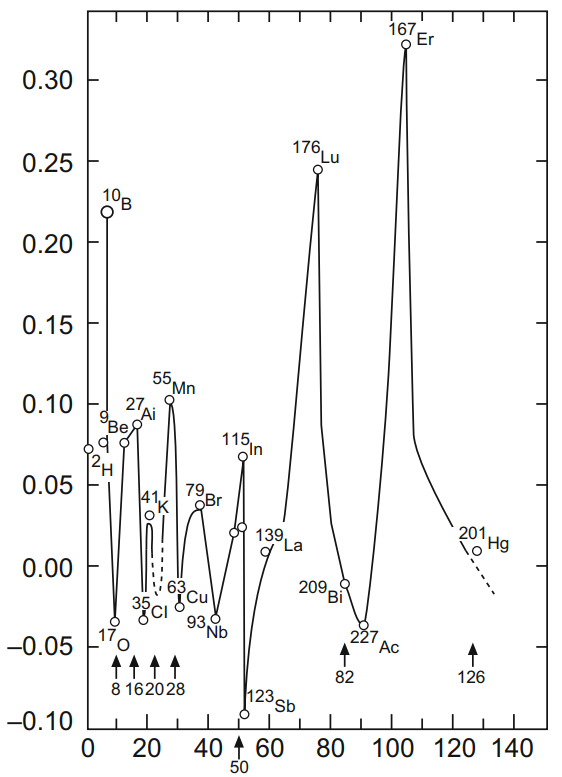
\includegraphics[width=\linewidth]{Diagramas Tema 3/Momentos cuadrupolares de los nucleos.png}
    \captionof{figure}{Momentos cuadrupolares reducidos para núcleos con número impar de protones \( Z \) o neutrones \( N \) graficados en función de este número.}
    \label{fig: momentos quadrupolares}
\end{minipage}

\section{Masa de los núcleos. Fórmula semiempírica de masas} 
Vamos a definir la masa de un núcleo como 
\begin{equation}
    M_\mathrm{nucleo}c^2=m(^A_Z X_N)c^2-Zm_ec^2+\sum_{i=1}^Z  
 B_i^e
 \label{eq: masa de un nucleo}
\end{equation}
donde $m(^A_Z X_N)$ es la masa del átomo (no del núcleo) y $B_i^e$ es la energía de ligadura que siente cada uno de los electrones, este término es despreciable ya que estas energía son del orden de los rayos X $(\unit[10-100]{keV})$ y la masa de un nucleón es del orden de los GeV.
\subsection{Energías de ligadura y de separación}
De manera análoga para el caso de los átomos, la energía de ligadura de un núcleo la definimos como 
\begin{equation}
    B(^A_Z X_N)=\qty[Z m(^1\mathrm{H})+Nm_n- m(^A_Z X_N)]c^2
    \label{eq: energia de ligadura}
\end{equation}

\begin{tcolorbox}[colback=applegreen!20, colframe=applegreen, title={Definición: Unidad de masa atómica}]
    Definimos la unidad de masa atómica como 
    \begin{equation*}
        \unit[1]{uma}=\frac{m\qty(^{12}\mathrm{C})}{12}
    \end{equation*}
\end{tcolorbox}

Podemos expresar la unidad de masa atómica en MeV, resultando $\unit[1]{uma}=\unit[931.5]{MeV}$, es decir, dentro del núcleo los nucleones son más ligeros por la energía de ligadura.\\\\
Definimos la energía de ligadura por nucleón como $\dfrac{B}{A}$ y el defecto de masa de un núcleo como 
\begin{equation}
    ^A \Delta = m(^A_Z X_N)c^2-\unit[A]{[uma]}
    \label{eq: defecto de masa}
\end{equation}

\begin{figure}[h]
        \centering
    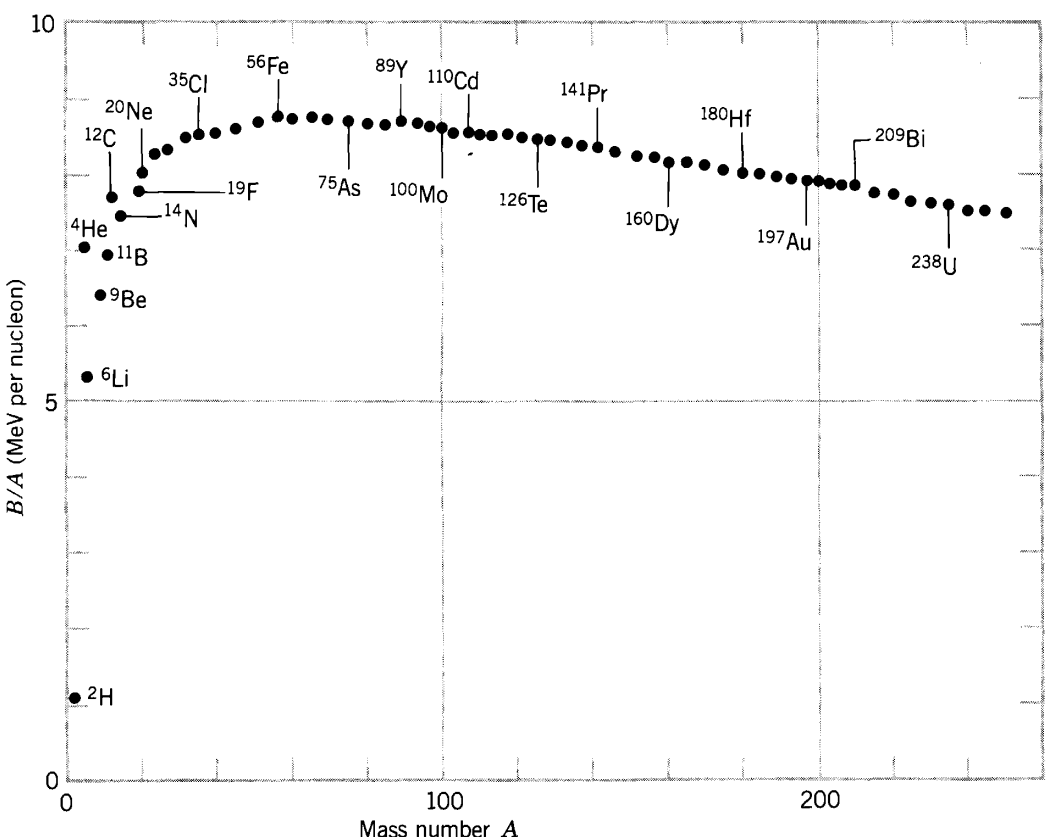
\includegraphics[width=\linewidth]{Diagramas Tema 3/Energia de ligadura por nucleon.png}
    \caption{Energía de ligadrua por nucleón en función del número de nucleones. Como vemos el núcleo de carbono-12 está fuera de la curva, al igual que las el núcleo de $^4$He (partícula $\alpha$).}
    \label{fig: energia de ligadura por nucleon frente al numero masico}
\end{figure}

Podemos utilizar el defecto de masa para saber cómo es la robustez del núcleo atómico, si el núcleo tiene mayor defecto de masa el núcleo estará más ligado que el átomo de $^{12}$C y viceversa
    $$\left \{ \begin{aligned}
        &^A \Delta >0 \xrightarrow[]{} \frac{B}{A}(^A_Z X_N)< \frac{B}{A}(^A_Z \mathrm{C})\\
        &^A \Delta <0 \xrightarrow[]{} \frac{B}{A}(^A_Z X_N)> \frac{B}{A}(^A_Z \mathrm{C})
    \end{aligned}   \right.$$

Si analizamos la figura \ref{fig: energia de ligadura por nucleon frente al numero masico} la energía es más o menos constante $\nicefrac{B}{A}\sim \unit[8]{MeV}$ salvo para núcleos ligeros. Esta curva tiene un máximo en $A\approx 60$, por lo que los núcleos atómicos que tienden a llegar a  este estado liberan energía de dos maneras
\begin{itemize}
    \item Para $A<60$ la energía de enlace por nucleón aumenta cuando añadimos nucleones, lo que conocemos como \textbf{fusión}.
    \item Para $A>60$ Aumentamos la energía de ligadura fraccionando los núcleos, lo que conocemos como \textbf{fisión}.
\end{itemize}

    Otra energía que podemos definir es la energía de separación, que es la energía que tenemos que darle a un núcleo para arrancarle un protón o un neutron.
    \begin{equation}
        \left \{  \begin{aligned}
    & S_n=\qty[m\qty(^{A-1}_Z X_{N-1})+m_n-m(^A_Z X_N)]c^2=B\qty(^A_Z X_N)-B\qty(^{A-1}_Z X_{N-1})\\
    &S_p=\qty[m\qty(^{A-1}_{Z-1} X_{N})+m\qty(^1\mathrm{H})-m(^A_Z X_N)]c^2=B\qty(^A_Z X_N)-B\qty(^{A-1}_{Z-1} X_{N})
        \end{aligned}
        \right.
        \label{eq: energías de separacion para el neutron y el proton}
    \end{equation}
    Este concepto es análogo a las energías de ionización en un átomo.\\
    \begin{tcolorbox}[colback=airforceblue!20, colframe=airforceblue, title={Ejemplo: Fusión del Deuterio en Helio-4}]
    Dada la siguiente reacción
    \begin{equation*}
        ^2\mathrm{H}+^2\mathrm{H} \longrightarrow ^4\mathrm{He}
    \end{equation*}
    Si hacemos uso de la ecuación \ref{eq: masa de un nucleo} y comparamos las energías de ambos miembros de la reacción, para el primer miembro tenemos  $2\qty(m_p+m_n-B_{^2\mathrm{H}})$ mientras que en el segundo $2m_p+2m_n-B_{^4\mathrm{He}}$, como las masas de los nucleones contribuyen de igual manera, la energía obtenida de la reacción es la diferencia de las energías de ligadura, como $\unit[B_{^2\mathrm{H}}=4.4]{MeV}$ y $\unit[B_{^4\mathrm{He}}=28]{MeV}$ obtenemos $\unit[24]{MeV}$ de la reacción.
\end{tcolorbox}

\subsection{Fórmula semiempírica de masas (Weizsäcker)}

Para intentar reproducir la curva que aparece en la figura \ref{fig: energia de ligadura por nucleon frente al numero masico} vamos a introducir la fórmula semiempírica de masas, esta fórmula no es reproducible por ningún (único) modelo nuclear. .\\\\

En lo primero que tenemos que pensar es cómo interaccionan los nucleones dentro del núcleo, volviendo a la figura \ref{fig: energia de ligadura por nucleon frente al numero masico}, vemos que a partir de $A=15$ la energía por nucleón varía entre $ \unit[[7.4,8.8]]{MeV}$, es decir, no es exactamente constante (como sí lo sería si todos los nucleones interaccionasen con todos) por lo que diremos que la interacción nuclear \textbf{satura}. 
\\\\
Veamos los términos que ha de tener la fórmula semiempírica de masas:
\begin{itemize}
    \item \textbf{Término de volumen} $a_\mathrm{V}A$: Como la interacción nuclear satura, la densidad del núcleo es \textbf{constante}, esto implica que cada nucleón tiene el mismo número de vecinos y cada nucleón contribuye a $B$ con la misma intensidad. Como hemos dicho que la densidad es constante y el núcleo es más o menos esférico, el volumen va como $R^3=R_0^3A$ la energía debe seer proporcional a $A$.
    \item \textbf{Término de superficie} $a_\mathrm{S}A^{2/3}$: Los nucleones que se encuentran en la superficie no tienen el mismo número de vecinos que los que se encuentran dentro del núcleo por lo que están menos ligados. Esta contribución resta (ya que estaríamos contando de más), y de manera análoga al término de volumen, la superficie de la esfera va como $R^2=R_o^2A^{2/3}$, este término ha de ser proporcional a $A^{2/3}$.
    \item \textbf{Término de Coulomb} $a_\mathrm{C}Z(Z-1)A^{-1/3}$: Los protones se repelen entre sí debido a la fuerza de Coulomb. Si hay $Z$ protones todos se repelen entre sí, luego el término es proporcional a $Z(Z-1)$. Si asumimos que la distribución de la carga es uniforme:
    \begin{equation}
        E_\mathrm{C}=-\frac{3}{5} \frac{e^2}{4\pi\varepsilon_0} \frac{Z(Z-1)}{R}=-\frac{3}{5} \frac{e^2}{4\pi\varepsilon_0} \frac{Z(Z-1)}{R_0A^{1/3}}
    \end{equation}
    Este término también resta (ya que separa los nucleones) y es proporcional a $Z(Z-1)A^{-1/3}$.
    \item \textbf{Término de simetría} $a_\mathrm{sym}\dfrac{(A-2Z)^2}{A}$: En la figura \ref{fig: Diagrama Segre} (plot de Segre) los núcleos con $A<40$ son simétricos, es decir, $N\approx Z \approx \nicefrac{A}{2}$. Por encima de este valor $\nicefrac{Z}{A}\approx \nicefrac{1}{2}$. Por lo que este término es cero si $Z=\nicefrac{A}{2}$ y su importancia decrece con $A$.\\\\
    Este término tiene gran relevancia en los núcleos pesados, pues de no existir tendríamos núcleos con un número infinito de neutrones.
    \item \textbf{Término de apareamiento} $\delta$: Tiene en cuenta la tendencia observada de los nucleones a agruparse por parejas. Si $A$ es impar el término no contribuye. Si $A$ es par tenemos dos posibilidades:
    \begin{itemize}
        \item Si $Z$ y $N$ son impares $B$ aumentará al transformar un neutrón en un protón o viceversa.
        \item Si $Z$ y $N$ disminuye $B$ al transformar un nucleón en otro.
    \end{itemize}
    Podemos parametrizarlo mediante la siguiente función \footnote{El exponente también puede ser $-\nicefrac{3}{4}$}
    \begin{equation}
        \delta = \left \{ \begin{aligned}
            &- a_\mathrm{p}A^{-1/2}  & \quad \text{si} \quad \text{(I,I)}\\
            &0 & \quad \text{si} \quad \text{(I,P) ó (P,I)} \\
            & a_\mathrm{p}A^{-1/2} & \quad \text{si} \quad \text{(P,P)}
        \end{aligned} \right.
    \end{equation}
    \label{eq: termino de pairing}
\end{itemize} 

Así la fórmula semiempírica de masas será
\begin{equation}
    \begin{aligned}
        &m(^A_Z X_N)c^2=\qty[Z m(^1\mathrm{H})+Nm_n]c^2-B(^A_Z X_N) \quad \mathrm{con} \\
        &B(^A_Z X_N)=a_\mathrm{V}A-a_\mathrm{S}A^{2/3}-a_\mathrm{C}\frac{Z(Z-1)}{A^{1/3}}-a_\mathrm{sym} \frac{(A-2Z)^2}{A}+\delta(A)
    \end{aligned}
    \label{eq: formulas semiempirica de masas}
\end{equation}


Fijémonos que esta ecuación \textbf{no considera los números mágicos}, por lo que en sus proximidades observaremos fluctuaciones.\\\\
La fórmula semiempírica de masas incorpora características individuales y globales de los núcleos, los 3 primeros términos considera al núcleo un ente global (partícula única), mientras que los 2 últimos hemos utilizado propiedades de los constituyentes (nucleones).

\begin{table}[h]
\centering
\begin{tabular}{|ccccc|}
\hline
\multicolumn{1}{|c|}{$a_\mathrm{V}$} &
  \multicolumn{1}{c|}{$a_\mathrm{S}$} &
  \multicolumn{1}{c|}{$a_\mathrm{C}$} &
  \multicolumn{1}{c|}{$a_\mathrm{sym}$} &
  $a_\mathrm{p}$ \\ \hline \hline
$\unit[15.67]{MeV}$ &
  $\unit[17.23]{MeV}$ &
  $\unit[0.72]{MeV}$ &
  $\unit[23.287]{MeV}$ &
  $\unit[12 \footnotemark]{MeV}$ \\ \hline
\end{tabular}
\caption{Valor de las constantes de la fórmula semiempírica de masas.}
\label{tab: constantes de Formula semiempirica de masas}
\end{table}
\footnotetext{En el caso de utilizar el exponente $-\nicefrac{3}{4}$, el valor de esta constante es $a_\mathrm{p}=\unit[34]{MeV}$}
\section{Inestabilidad nuclear}
La fórmula semiempírica de masas nos permite analizar la estabilidad de los núcleos, así como en qué modos va hacia la estabilidad. Si tenemos una reacción $$a+A\longrightarrow b+B$$
Definimos el \textbf{factor \textit{Q}} como 
\begin{equation}
    Q=\qty[M(a)+M(A)-M(b)-M(B)]c^2 \left \{ \begin{aligned}
        &Q>0 \quad \text{Exotérmica}\\
        &Q<0 \quad \text{Endotérmica}
    \end{aligned} \right.
    \label{eq: factor Q}
\end{equation}
Para el caso de las desintegraciones, la reacción tiene la forma $A\xrightarrow[]{} b+c+\cdots$ y para que se produzcan de manera espontánea $Q>0$
\subsection{Tipos de desintegraciones radiactivas} \label{sec: Tipos de desintegraciones radiactivas}
\begin{itemize}
    \item \textbf{Desintegración $\bm{\alpha}$}: El núcleo emite una partícula $\alpha\equiv\, ^{\ 4}\mathrm{He}$. La desintegración tiene la forma 
    \begin{equation*}
        ^A _Z X_N \longrightarrow ^{A-4} _{Z-2} Y_{N-2}+ ^4\mathrm{He}
    \end{equation*}
        
    Como vimos en el apéndice \ref{chap: Apendice B}, por ser una desintegración a dos cuerpos (no relativista + relativista) con la energía de las partículas $\alpha$ está \textbf{discretizada}.
    \item \textbf{Desintegración $\bm{\beta^-}$}: El núcleo corrige el exceso de neutrones transformando un neutrón en un protón y emitiendo el electrón resultante junto con un antineutrino
    \begin{equation*}
        ^A _Z X_N \longrightarrow ^{\ \ \ A} _{Z+1} Y_{N-1}+ e^-+\Bar{\nu}_e
    \end{equation*}

        Por ser una desintegración a tres cuerpos (2 relativistas + 1 pesado) el electrón presenta un espectro continuo de energías.

    \item \textbf{Desintegración $\bm{\beta^+}$}:  El núcleo corrige el exceso de protones transformando un neutrón en un protón y emitiendo el positrón resultante junto con un neutrino
    \begin{equation*}
        ^A _Z X_N \longrightarrow ^{\ \ \ A} _{Z-1} Y_{N+1}+ e^++{\nu}_e
    \end{equation*}

    De igual menera, el positrón presenta un espectro contínuo de energías \ref{fig: Emisioones electrones}

    \item \textbf{Captura electrónica}: El núcleo corrige un exceso de protones absorbiendo un electrón atómico y emitiendo el neutrino correspondiente
    \begin{equation*}
        ^A _Z X_N +e^- \longrightarrow ^{\ \ \ A} _{Z-1} Y_{N+1}++{\nu}_e
    \end{equation*}

    Esto compite con la desintegración $\beta^+$, pero sólo en los casos en los que tenemos $M_X-M_Y<2m_e$ ya que si no se cumpliese no se conserva la energía y estaría prohibido.

    \item \textbf{Desintegración $\bm{\gamma}$}: Un núcleo de un estado excitado se desintegra a su estado fundamental emitiendo un fotón 
    $${^A _Z X_N }^*\longrightarrow ^A _Z X_N+\gamma$$
    
    El espectro de los fotones emitidos es \textbf{discreto}.
    
    \item \textbf{Conversión interna}: El núcleo en un estado excitado se desintegra a su estado fundamental transfiriendo energía a un electrón atómico que es expulsado.
    $${^A _Z X_N }^*\longrightarrow ^A _Z X_N+e^-$$

    Esta desintegración compite con la desintegración $\gamma$, y el espectro de los electrones emitidos es discreto, los electrones al reordenarse emiten rayos X con energías discretas.
    \item \textbf{Fisión espontánea}: Un núcleo pesado se fragmenta en dos núcleos más ligeros
    $${^A _Z X_N }^*\longrightarrow {^{A^\prime} _{Z^\prime} Y_{N^\prime}+ ^{A-A^\prime} _{Z-Z^\prime} Y_{N-N^\prime}  }$$
    La distribución de la masa de los núcleos resultantes sigue una  distribución asimétrica, por ejemplo, en la desintegración del $^{235} _{92} \mathrm{U} \longrightarrow ^{95}\mathrm{Kr}+^{137}\mathrm{Ba}$
    \item \textbf{Emisión de un nucleón}: Un nucleón expulsa el exceso de nucleones. Suele darse tras una fisión nuclear y es cómo se originan las reacciones en cadena en un reactor.
\end{itemize}

\section{Parábolas de estabilidad}
La fórmula semiempírica de masas \ref{eq: formulas semiempirica de masas} la podemos escribir como una parábola:
\begin{equation}
    M(A,Z)=\gamma Z^2-\beta Z + \alpha \quad \text{con} \quad \left \{ 
    \begin{aligned}
    &\gamma= \frac{a_\mathrm{C}}{A^{1/3}}+4\frac{a_\mathrm{sym}}{A} \\
    &\beta=-m_pc^2+m_nc^2-4a_\mathrm{sym}\qty(\frac{a_\mathrm{C}}{A^{1/3}}) \\
    &\alpha= m_nc^2-a_\mathrm{V} +a_\mathrm{S}A^{-1/3}+a_\mathrm{sym} + \frac{\delta}{A}
    \end{aligned} \right.
\end{equation}

Si fijamos $A$ y minimizamos la función $M(A,Z)$, obtenemos el elemento químico más estable para un $A$ dado.
\begin{equation}
    Z^\mathrm{Th}_\mathrm{min}=\frac{(m_n-m_p)c^2+4a_\mathrm{sym}}{2\frac{a_\mathrm{c}}{A^{1/3}}+8\frac{a_\mathrm{sym}}{A}}
    \label{eq: Z minimo para un A constante}
\end{equation}

Esta ecuación si $A$ es pequeño se comporta como $Z^\mathrm{Th}_\mathrm{min} \xrightarrow[]{} A/2$; si $A$ es grande $Z^\mathrm{Th}_\mathrm{min}<A/2$; y para $A$ muy grandes $Z^\mathrm{Th}_\mathrm{min}/A\approx 0.4 $.
\subsubsection{Parábolas de estabilidad. Núcleos impares}
    Los núcleos impares se desplazan sobre la parábola de estabilidad a través de las desintegraciones fundamentales $\textcolor{blue}{\beta^-}$, $\textcolor{applegreen}{\beta^+}$ ó \textcolor{applegreen}{CE}; hasta alcanzar el valor $Z_\mathrm{min}$.
\subsubsection{Parábolas de estabilidad. Núcleos Pares}
    En el caso de los núcleos pares tendreemos dos núcleos estables para un $A$ fijo, uno con vida media infinita (estable) y otro con vida media muy larga, que sólo se podría desintegrar por doble desintegración $\beta$ (línea punteada de la figura \ref{fig: Parabola Estabilidad A par})
\begin{figure}[h]
    \begin{subfigure}{0.45\textwidth}
            \centering
    \includegraphics[width=\linewidth]{Diagramas Tema 3/ParabolaEstabilidadAimpar.pdf}
    \caption{Parábola de estabilidad para $A$ impar.} 
    \label{fig: Parabola Estabilidad A impar}
    \end{subfigure}
    \hfill
    \begin{subfigure}{0.45\textwidth}
            \centering
    \includegraphics[width=\linewidth]{Diagramas Tema 3/ParabolaEstabilidadApar.pdf}
    \caption{Parábolas de estabilidad para $A$ par.} 
    \label{fig: Parabola Estabilidad A par}
    \end{subfigure}
    \caption{Parábolas de estabilidad.}
\end{figure}
\pagestyle{fancy}
\fancyhead[R]{Física Nuclear y de Partículas: Tema 4}
\fancyhead[L]{4º Grado en Física}
\chapter{Inestabilidad Nuclear}

\section{Radiactividad natural y desintegración nuclear}
Es lícito pensar que el origen de la física nuclear se debe a las emisiones radiactivas de los minerales naturales de $$\begin{aligned}
    & ^{238} _{92} \mathrm{U} \xrightarrow{} t_\mathrm{\nicefrac{1}{2}}\sim \unit[4.5\cdot10^{9}]{year}\\
    &^{232} _{90} \mathrm{Th} \xrightarrow{} t_\mathrm{\nicefrac{1}{2}}\sim \unit[14.1\cdot10^{9}]{year}
\end{aligned}$$
Cuyas vidas medias son del orden de la edad de la Tierra.
La radiactividad artificial nace en 1934 cuando Irene y Frederic Joliot-Curie produjeron el $^{13} _7\mathrm{N}^*$, un núcleo inestable que no existe en la naturaleza, a través de la reacción
$$\alpha + ^{10} _{\ 5} \mathrm{B}\longrightarrow \textcolor{red}{^{13} _{\ 7}\mathrm{N}^*} +n \textcolor{red}{\longrightarrow ^{13} _{\ 6}\mathrm{C}+ e^++\nu_e}$$
En 1930 sintetizarán el $^{30}\mathrm{P}$: 
$$\alpha + ^{27} _{13} \mathrm{Al}\longrightarrow \textcolor{red}{^{30} _{15}\mathrm{P}^*} +n \textcolor{red}{\longrightarrow ^{30} _{14}\mathrm{Si}+ e^++\nu_e}$$

Este tipo de estudios permitieron descubrir cuatro elementos no detectados, el Tecnecio, Prometio, Astato y Francio; sin tienen isótopos estables. Como dato existen más de 40 elementos en la corteza terrestre que son radiactivos.

\subsection{Ley de desintegración radiactiva}
Poco después de descubrirse la existencia de la radiactividad se observó que la tasa de desintegración disminuye exponencialmente con el tiempo. Vamos a definir una serie de conceptos relevantes en el estudio de la inestabilidad nuclear\\\\
Definimos la \textbf{actividad} de una muestra , $A$, como el número de núcleos que se desintegran por unidad de tiempo. Si $N$ es el número de átomos de un radionucleido en el instante $t$, entonces 
\begin{equation}
    \dv{N(t)}{t}=-\lambda N(t) \Rightarrow N(t)=N_0\exp{-\lambda t}
    \label{eq: ley de desintegracion radiactiva}
\end{equation}

Donde $\lambda$ es la constante de desintegración, ésta se define como la probabilidad de desintegración de un núcleo por unidad de tiempo, esta constante se caracteriza por 
\newpage
\begin{itemize}
    \item Ser independiente de $t$.
    \item No podemos decir cuándo un núcleo va a desintegrarse, pero si podemos describir el comportamiento de un gran número de núcleos idénticos.
\end{itemize}
Por lo tanto la actividad la definimos como 
\begin{equation}
    A(t)=-\dv{N(t)}{t}=\lambda N(t) =\lambda N_0 \exp{-\lambda t}\Rightarrow [A(t)]\equiv \unit[1]{Bq}=\unit[1]{desintegracion/s}
    \label{eq: actividad radiactiva}
\end{equation}
Como el Bequerelio (Bq) es una unidad muy pequeña, se toma el Curio (Ci) como unidad de medida en una desintegración, esta unidad se define como $$\unit[1]{Ci}=\unit[3.7\cdot 10^{10}]{Bq}$$

Definimos \textbf{semivida} como el periodo de tiempo necesario para que se desintegre la mitad de la muestra
\begin{equation}
    A(t_{\nicefrac{1}{2}})=\frac{A_0}{2} \xrightarrow{} \frac{A_0}{2}=A_0\exp{-\lambda t_{\nicefrac{1}{2}}} \Rightarrow \boxed{t_{\nicefrac{1}{2}}=\frac{\log 2}{\lambda}} \footnotemark
    \label{eq: semivida}
\end{equation}
\footnotetext{log es el logaritmo natural, el logaritmo en base 10 lo denotaré como $\log_{10}$.}

Definimos \textbf{vida media} como el promedio de tiempo  que un núcleo individual tarda en desintegrarse
\begin{equation}
    \tau=\displaystyle \dfrac{ \displaystyle\int_0^\infty t \abs{\dv{N}{t}}\dd t}{ \displaystyle\int_0^\infty  \abs{\dv{N}{t}}\dd t}= \dfrac{ \displaystyle \int^\infty_0 t \exp{-\lambda t}}{ \displaystyle\int^\infty_0  \exp{-\lambda t}}=\frac{1}{\lambda}=\frac{t_{\nicefrac{1}{2}}}{\log 2}
    \label{eq: Vida media}
\end{equation}

Definimos \textbf{actividad específica} como la actividad por unidad de masa
\begin{equation}
    A^\prime =\frac{A}{m}=\lambda \frac{N_A}{M_\mathrm{At}}
    \label{eq: activida especifica}
\end{equation}

Ahora supongamos que tenemos una cadena de desintegración $N_0\xrightarrow[]{} N_1\xrightarrow[]{} N_2$, de una misma especie en este caso las desintegraciones de las especies $N_1$ y $N_2$ vienen dadas por 
\begin{equation*}
     \left. \begin{aligned}
        &N_1(t)=N_0\exp{-\lambda t}\\
        &N_2(t)=N_0\qty(1-\exp{-\lambda t})
    \end{aligned} \right \} N_1(t)+N_2(t)=N_0
\end{equation*}

Normalmente un núcleo se desintegra en varios estados finales. En este caso, cada desintegración estará caracterizado por una constante $\lambda_i$, así la desintegración de una sustancia será 
\begin{equation}
    \eval{\dv{N}{t}}_\mathrm{Total}=\sum_i \eval{\dv{N}{t}}_i=-N\sum_i\lambda_i=-N \lambda_\mathrm{Total} \Rightarrow \boxed{N(t)=N_0\exp{-\lambda_\mathrm{Total}t}}
\end{equation}
Para el caso de los productos, tenemos
\begin{equation}
    N_{i}(t)=N_0 \frac{\lambda_i}{\lambda_\mathrm{Total}}(1-\exp{-\lambda_\mathrm{Total}t})=N_0BR_i (1-\exp{-\lambda_\mathrm{Total}t})
\end{equation}
\newpage
\subsection{Producción y desintegración de radionucleidos. Radiactividad artificial}
Los radionucleidos se producen a través de \textbf{bombardeo nuclear}.\\\\
Supongamos que tenemos una placa de $^{23}\mathrm{Na}$ hiperpuro sobre la que incidimos con un haz de deuterones, con ello produciremos la siguiente reacción:
\begin{equation*}
    ^{23}\mathrm{Na} + ^{\ 2}\mathrm{H}\longrightarrow \textcolor{red}{^{24}\mathrm{Na}} + ^{\ 1}\mathrm{H} \textcolor{red}{\xrightarrow[]{\ \lambda_1 \ } \,^{24}\mathrm{Mg}+e^-+\Bar{\nu}_e }
\end{equation*}
La tasa de producción del radionucleido $^{24}\mathrm{Na}$ será $R=N_{0}\phi\sigma$. Como el número de partículas que hay en la placa es del orden (incluso superior) del número de Avogadro,  podemos suponer que la cantidad de  núcleos padres es constante; por otro lado, la sección eficaz del haz es $\sigma=\unit[1]{b}=\unit[10^{-24}]{cm^{-2}}$, mientras que el flujo de deuterones es de $\phi=\unit[10]{cm^{-2}\,s^{-1}}$ por lo tanto tenemos que la probabilidad de producción será $\phi \sigma =\unit[10^{-10}]{s^{-1}}\equiv \unit[10^{-6}]{hour^{-1}}$, con lo que asumimos que la tasa de producción es constante.\\\\
La expresión que nos da la tasa de producción en función del tiempo es

\begin{equation}
    \dd N_{^{24}\mathrm{Na}}=R\dd t-\lambda_1N_{^{24}\mathrm{Na}}\dd t \Rightarrow N_{^{24}\mathrm{Na}}=\frac{R}{\lambda_1}\qty(1-\exp{-\lambda_1 t})
    \label{eq: tasa de produccion}
\end{equation}

En función del tiempo de irradiación, tenemos tres regímenes diferentes\\
\noindent 
\begin{minipage}{0.6\textwidth}
\begin{itemize}
    \item $t\ll t_{\nicefrac{1}{2}} \Rightarrow A_{^{24}\mathrm{Na}} \simeq R\lambda_1t$
    \item $t\gg t_{\nicefrac{1}{2}} \Rightarrow A_{^{24}\mathrm{Na}} \simeq R$
    \item Cuando se produce la desconexión del haz incidente $t=t_{\mathrm{des}} \Rightarrow A_{^{24}\mathrm{Na}}\simeq R\qty(1-\exp{-\lambda_1 t_\mathrm{des}}) \exp{-\lambda_1(t-t_\mathrm{des})}$
\end{itemize}
\end{minipage}
\hfill
\begin{minipage}{0.35\textwidth}
    \centering
    \includegraphics[width=\linewidth]{Diagramas Tema 4/Actividadmuestra radiada.pdf}
    \captionof{figure}{Diferentes regímenes de actividad de una muestra.}
    \label{fig: actividad de una muestra}
\end{minipage}
\\\\
Los radionucleidos tienen infinidad de aplicaciones, aunque las más conocidas son las aplicaciones médicas.
\subsection{Series radiactivas. Ecuaciones de Bateman}
En la naturaleza los núcleos hijos son estables y se desintegran en otra serie de productos, supongamos que tenemos una cadena de desintegraciones compuesta por tres especies
$$N_1\xrightarrow[]{\ \lambda_1\ } N_2 \xrightarrow[]{\ \lambda_2 \ } N_3$$
Estudiemos la variación de las distintas especies nucleares
\begin{equation}
    \dv{N_1}{t}=-\lambda_1 N_1, \quad \dv{N_2}{t}=\lambda_1 N_1-\lambda_2 N_2, \quad \dv{N_3}{t}=\lambda_2 N_2
    \label{eq: variaciones serie de desintegracion}
\end{equation}

Estamos en el caso más general, por lo que supondremos que en $t=0$ tenemos $N_{1,0},N_{2,0},N_{3,0}$ partículas de cada una de las especies. Cada una de estas ecuaciones tendrá solución

\begin{equation}
    N_1(t) = N_{1,0} \exp{-\lambda_1 t}
    \label{eq: desintegracion nucleo padre}
\end{equation}

\begin{equation}
    N_2(t) = N_{1,0} \frac{\lambda_1}{\lambda_2 - \lambda_1} 
    \qty(\exp{-\lambda_1 t} - \exp{-\lambda_2 t}) 
    + N_{2,0} \exp{-\lambda_2 t}
    \label{eq: desintegracion nucleo hijo inestable}
\end{equation}

\begin{equation}
    \begin{aligned}
        N_3(t) = & N_{1,0} \qty(1 + \frac{1}{\lambda_2 - \lambda_1}
        \qty(\lambda_1 \exp{-\lambda_1 t} - \lambda_2 \exp{-\lambda_2 t})) \\
        & + N_{2,0} \qty(1 - \exp{-\lambda_2 t}) + N_{3,0}
    \end{aligned}
    \label{eq: desintegracion nucleo nieto estable}
\end{equation}

Para tiempos $t\ll t_{\nicefrac{1}{2},1}\  (\lambda_2\gg \lambda_1)$ podemos considerar que la actividad de la especie $N_1$ es constante y decimos que las especies están en \textbf{equilibrio secular}, si además tenemos que $t\gg t_{\nicefrac{1}{2},2}$ tendremos que $\dfrac{A_2}{A_1} \approx 1$ , en la figura \ref{fig: actividad de una muestra}, es el valor máximo que alcanza la actividad. \\\\
Si consideramos tiempos  $t > t_{\nicefrac{1}{2},1}\  (\lambda_2> \lambda_1)$ las actividades de los núcleos pares e hijos son proporcionales después de cierto tiempo transcurrido.\\\\
Si calculamos el cociente entre las actividades de las especies $N_2$ y $N_1$, a partir de las ecuaciones \ref{eq: desintegracion nucleo hijo inestable} y \ref{eq: desintegracion nucleo padre} tenemos
\begin{equation*}
    \frac{A_2}{A_1}=\frac{\lambda_2}{\lambda_2-\lambda_1}\qty(1-\exp{-(\lambda_2-\lambda_1)t})
\end{equation*}
Recuperando la condición $\lambda_2 > \lambda_1$ tenemos que para $t\gg  \dfrac{1}{\lambda_2-\lambda_1}$ podemos aproximar el cociente por $$\frac{A_2}{A_1}=\frac{\lambda_2}{\lambda_2-\lambda_1}\approx 1$$
Esta ultima igualdad es lo que se conoce como \textbf{equilibrio tansitorio}. \\\\
Por último tenemos la situación en la que $\lambda_2<\lambda_1$, en este caso el cociente entre actividades será:
\begin{equation*}
    \frac{A_2}{A_1}=\frac{\lambda_2}{\lambda_2-\lambda_1}\qty(1-\exp{-(\lambda_2-\lambda_1)t}) \xrightarrow[]{\lambda_2<\lambda_1} \frac{A_2}{A_1}=\frac{\lambda_2}{\abs{\lambda_2-\lambda_1}}\qty(\exp{(\lambda_2-\lambda_1)t}-1)
\end{equation*}
Que para $t\gg t_{\nicefrac{1}{2},1}$ la actividad de la especie $N_2$ es 
\begin{equation*}
    A_2(t)=A_{1,0}\frac{\lambda_2}{\lambda_1-\lambda_2}\exp{-\lambda_2t}
\end{equation*}

A esta situación se le conoce como \textbf{no equilibrio}.

\subsubsection{Ecuaciones de Bateman}
Las expresiones anteriores se pueden extender al caso general de cadenas con varias generaciones de desintegraciones nucleares. El caso general es 
\begin{equation}
    N_1\xrightarrow[]{\lambda_1} N_2 \xrightarrow[]{\lambda_2} \cdots \xrightarrow[]{\lambda_{n-1}} N_n
    \label{eq: cadena general}
\end{equation}

Y la actividad del $n$-ésimo radionucleido es 
\begin{equation}    A_n(t)=N_{1,0}\Bigg(\prod_{i=1}^n\lambda_i\Bigg)\Bigg(\sum_{k=1}^n\frac{e^{-\lambda_kt}}{\prod_{j=1}^n\left(\lambda_j-\lambda_k\right)}\Bigg)
\label{eq: actividad del nesimo nucleido de una cadena radiactiva}
\end{equation}

Para el caso del equilibrio secular tenemos $$A_1(t)=A_2(t)=\cdots = A_{n-1}(t)$$

\subsection{Radiactividad natural}
Algunos de los elementos naturales que constituyen la corteza terrestre son radiactivos (unos 40). Una parte procede de elementos formados junto con la Tierra, y que debido a su larga vida media aún son medidos; y otra procede de los núcleos hijos productos de los desintegrados. Otra componente está formada por elementos producidos en colisiones de rayos cósmicos con los núlceosde la atmósfera.\\\\
La radiactividad natural de origen terrestre es debida en su mayor parte a las desintegraciones de las cadenas de elementos pesados (tranuránidos, $Z>83$). De ellos únicamente el radón supone un problema serio para la salud.\\\\
La mayoría de elementos pesados se desintegran por dos canales: $\alpha$ y $\beta$. Esto nos permite definir cuatro series de desintegraciones fundamentales: $^{232}\mathrm{Th}(4n), ^{241}\mathrm{Np}(4n+1), ^{238}\mathrm{U}(4n+2), ^{241}\mathrm{U}(4n+3)$, debido a que la vida media del $^{241}\mathrm{Np}$ es ``sólo'' de 2 millones de años, esta cadena ya no existe de forma natural en la Tierra.
\subsection{Datación radiométrica: Carbono-14}

El $^{14}\mathrm{C}$ se forma constantemente en la atmósfera debido a la acción de los rayos cósmicos. $$ _{\ 7}^{14}\mathrm{N} +n \longrightarrow{} _{\ 6} ^{14} \mathrm{C}+p$$

De tal forma que la composición isotópica del C en nuestro planeta es de $98.89\%$ de $^{12}\mathrm{C}$, $1.11\%$ de $^{13}\mathrm{C}$ y $10^{-10}\%$ de $^{14}\mathrm{C}$.\\\\
Un organismo vivo absorbe $^{14}\mathrm{C}$ durante toda su vida. Cuando muere, deja de introducir carbono-14 nuevo y el que posee sólo se desintegra. Por lo tanto, midiendo su actividad podemos obtener la fecha de fallecimiento. Si denominamos al tiempo de fallecimiento como $t_0$ a partir de la ecuación \ref{eq: ley de desintegracion radiactiva} tenemos 
$$N_{^{14}\mathrm{C}}(t)=N_{^{14}\mathrm{C}}(t_0) \exp{-\lambda (t-t_0)} \Rightarrow \Delta t= t-t_0= \frac{t_{\nicefrac{1}{2}}}{\log 2} \log(\frac{N_{^{14}\mathrm{C}}(t)}{N_{^{14}\mathrm{C}}(t_0)})$$

Recordemos que $t_{\nicefrac{1}{2}}({}^{14}\mathrm{C})=\unit[5730]{year}$, la intensidad de $^{14}\mathrm{C}$ deja de ser medible a partir de $t\approx 10 t_{\nicefrac{1}{2}}$, por lo tanto es aplicable entre 50 y 60000 años.\\\\ La datación por carbono-14 tiene varios problemas, debido a la quema de combustibles fósiles la concentración de $^{12}\mathrm{C}$ ha cambiado. Otro problema son las pruebas nucleares realizadas durante la Guerra Fría, lo que ha incrementado la concentración de $^{14}\mathrm{C}$ en la atmósfera.

\subsection{Datación radiométrica geológica: Rubidio-87}
Para medir escalas geológicas no podemos medir la actividad en función del tiempo, por lo que estudiamos la razón entre el núcleo padre y el núcleo hijo.\\\\
La más utilizada es la desintegración $\beta^- $ del $^{87}\mathrm{Rb}$ en $^{87} \mathrm{Rb}$. Una característica del Sr es que tenemos dos isótopos estables con una composición isotópica similar: $^{86}\mathrm{Sr}, ^{87}\mathrm{Sr}$.\\\\
Una primera posibilidad es suponer que en el instante de tiempo inicial, cuando la roca se formó, sólo existieran núcleos padre y que no han aparecido nuevos núcleos padre en todo el tiempo transcurrido. $$N_{^{86}\mathrm{Sr}}(t_\mathrm{hoy})+N_{^{86}\mathrm{Rb}}(t_\mathrm{hoy})=N_{^{86}\mathrm{Rb}}(t)$$ Recuperando de nuevo la ecuación \ref{eq: ley de desintegracion radiactiva} vemos que 
$\Delta t=\dfrac{t_{\nicefrac{1}{2}}}{\log 2} \log(1+\dfrac{N_{^{87}\mathrm{Sr}}(t)}{N_{^{87}\mathrm{Rb}}(t_0)})$\\\\
Supongamos ahora que cuando se formó la roca existieran núcleos hijos en el material, 
$$N_{^{86}\mathrm{Sr}}(t_\mathrm{hoy})+N_{^{86}\mathrm{Rb}}(t_\mathrm{hoy})=N_{^{86}\mathrm{Rb}}(t)+N_{^{86}\mathrm{Sr}}(t)$$
En este caso la expresión anterior no es vlaída. Lo que hacemos es utilizar otro isótopo estable del núcleo hijo $N_{^{86}\mathrm{Sr}}(t_\mathrm{hoy})=N_{^{86}\mathrm{Sr}}(t_0)$. Obteniendo $$\frac{N_{^{87}\mathrm{Sr}}(t_\mathrm{hoy})}{N_{^{86}\mathrm{Sr}}(t_\mathrm{hoy})}=m\frac{N_{^{86}\mathrm{Sr}}(t_\mathrm{hoy})}{N_{^{87}\mathrm{Rb}}(t_\mathrm{hoy})}+b$$
El procedimiento consiste en localizar rocas con distintos minerales ricos en estroncio y midiendo la proporción de estroncio-87 y rubidio-87 respecto a la de estroncio-86 obtenemos una serie de puntos que ajustamos a una recta y su pendiente nos dará la edad.
\section{Desintegración beta. Modelo de Fermi}

La desintegración $\beta$ nuclear constituye la primera manifestación de la interacción débil y su estudio introdujo algunos de los cambios más significativos en la Física del siglo XX. Hacia 1920 se había establecido claramente la presencia de un espectro continuo de electrones de origen nuclear en la desintegración $\beta$ como consecuencia de ser una desintegración a 3 cuerpos. Además por ser producto de la interacción débil no conserva paridad.\\\\
Recordamos que la desintegración $\beta$ compite con la captura electrónica pero se diferencia de esta debido a la emisión de rayos X característicos.\\\\ 
En 1934 Fermi formula una teoría de la desintegración $\beta$ utilizando el neutrino y consigue explicar la forma de los espectros.
\newpage
\subsubsection{Balance energético. Estudio del factor \textit{Q}}
Esta sección corresponde al desarrollo de la sección \ref{sec: Tipos de desintegraciones radiactivas}. Recordando la definición del factor $Q$ dada por la ecuación \ref{eq: factor Q} \footnote{Tomaremos $c=1$ en esta sección para ahorrar términos y en el caso de ser necesarias se incluirán. También despreciaremos las energías de ligadura salvo cuando sea necesario.}
\begin{itemize}
    \item Desintegración $\beta^-$: De la reacción 
      \begin{equation*}
        ^A _Z X_N \longrightarrow {}^{A} _{Z+1} Y_{N-1}+e^-+\Bar{\nu}_e
        \end{equation*}
    Luego el factor $Q_{\beta^-}=m(^{A} _{Z}X_N )-\qty[ m({}^{A} _{Z+1} Y_{N-1})+ m_e- \textcolor{red}{m_e}\footnotemark ]$ Así para que se produzca una $\beta^-$ simplemente se necesita que la masa del átomo final sea menor que la del inicial. Si expresamos la definición del factor $Q_{\beta^-}$ en términos de la masa nuclear y la masa del electrón tenemos 
    \begin{equation*}
        \begin{aligned}
            Q_{\beta^-}=&\qty[m_\mathrm{Nuclear}({}^A_Z X_N)+Zm_e]-\qty[m_\mathrm{Nuclear}({}^A_{Z+1} Y_{N-1})+(Z+1)m_e-m_e]=\\ &m_\mathrm{Nuclear}({}^A_Z X_N)-m_\mathrm{Nuclear}({}^A_{Z+1} Y_{N-1})=m({}^A_Z X_N)-m({}^A_{Z+1} Y_{N-1})
        \end{aligned}
    \end{equation*}
    \item Desintegración $\beta^+$: De la reacción
          \begin{equation*}
        ^A _Z X_N \longrightarrow {}^{A} _{Z-1} Y_{N+1}+e^++\nu_e
        \end{equation*}
    Luego el factor $Q_{\beta^+}=m(^{A} _{Z}X_N )-\qty[ m({}^{A} _{Z-1} Y_{N+1})+ m_e+ \textcolor{red}{m_e}\footnotemark ]$. Si expresamos la definición del factor $Q_{\beta^-}$ en términos de la masa nuclear y la masa del electrón tenemos 
    \begin{equation*}
        \begin{aligned}
            Q_{\beta^-}=&\qty[m_\mathrm{Nuclear}({}^A_Z X_N)+Zm_e]-\qty[m_\mathrm{Nuclear}({}^A_{Z-1} Y_{N+1})+(Z-1)m_e+m_e]=\\ &m_\mathrm{Nuclear}({}^A_Z X_N)-m_\mathrm{Nuclear}({}^A_{Z-1} Y_{N+1})-2m_e= m({}^A_Z X_N)-m({}^A_{Z-1} Y_{N+1})-2m_e
        \end{aligned}
    \end{equation*}
    Este proceso sólo se dará si el núcleo padre y el núcleo hijo se diferencian en $2m_e\sim \unit[1]{MeV}$.
    \item Captura electrónica $\varepsilon$: De la reacción
    \begin{equation*}
        e^-+{} ^A _Z X_N\longrightarrow{} ^{A} _{Z-1}Y_{N+1} + \nu_e
    \end{equation*}
    Ahora sí que vamos a considerar la energía de ligadura, el factor $Q$ de la reacción es 
    \begin{equation*}
        Q_\varepsilon=m(^A _Z X_N)+m_e-m({} ^{A} _{Z-1}Y_{N+1})-B\approx m(^A _Z X_N)-m({} ^{\ \ A} _{Z-1}Y_{N+1})
    \end{equation*}
    Como la energía de ligadrua del electrón y la masa del electrón son del mismo orden, tenemos que la diferencia $m_ec^2-B\sim \unit[1]{keV}$ y lo podemos despreciar.
\end{itemize}
\footnotetext{Como la masa atómica es la masa de los átomos neutros debemos quitar ese electrón ya que la masa de $^{A} _{Z+1} Y_{N-1}$ está ionizado ya que tiene $Z$ electrones.}
\footnotetext{Al igual que antes tenemos que tener en cuenta la ionización de los átomos por lo que al tener este un protón menos que el núcleo padre tenemos que sumar la masa del nuevo electrón.}
\newpage
\subsection{Teoría de Fermi de la desintegración beta}

Como la desintegración $\beta$ de un núcleo es un proceso débil, consideraremos que estos procesos están en el régimen perturbativo dependiente del tiempo.\\\\
Partimos de un hamiltoniano $H_0$ responsable de los estados (quasi)\textbf{estacionarios}\footnote{Recordemos que los tiempos característicos de la interacción fuerte son del orden de $\unit[10^{-24}]{s}$ mientras que los de la interacción débil son superiores a $\unit[10^{-14}]{s}$ (Tabla \ref{tab: comparacion de escalas}) } nucleares y $H_1 =H_1(t)\equiv \alpha H_1$ con $\alpha \ll 1$ una perturbación dependiente del tiempo tal que $H=H_0+\alpha H_1$. \\\\ En un núcleo, la interacción dominante es la interacción fuerte, por lo que los estados iniciales, $\ket{\mathrm{i}}\equiv \chi_\mathrm{i}$ son propios del hamiltoniano de dicha interacción, por ser \textbf{estados ligados} presentan un espectro discreto. Las partículas ligeras producto de la desintegración las consideraremos \textbf{libres} por lo que tenemos \textbf{transiciones al continuo}.  Este tipo de transiciones vienen regidas por la regla de oro de Fermi (ecuación \ref{eq: regla de oro de fermi}) que tiene como expresión diferencial
\begin{equation*}
   \dd \lambda=\frac{2\pi}{\hbar} \abs{V_\mathrm{if}}^2 (4\pi)^2 \frac{\dd n_e \dd n_\nu}{\dd E_\mathrm{f}}
\end{equation*}
Los estados alcanzables \footnote{Como son partículas libres, el conjunto de estados alcanzable es una esfera de radio $p=\abs{\vec{p}}$ y tomando el diferencial de volumen $\dd V=4\pi p^2 \dd p$} por los leptones son
\begin{equation*}
    \left.\begin{aligned}
        &\dd n_e =\frac{4\pi p^2V\dd p}{h^3}\\
        &\dd n_{\Bar{\nu}} =\frac{4\pi q^2V\dd q}{h^3}
    \end{aligned} \right\} \Rightarrow \frac{\dd n_e \dd n_{\Bar{\nu}}}{\dd E_\mathrm{f}} = V^2 \frac{(4\pi)^2 p^2 q^2}{h^6} \frac{\dd p \dd q}{\dd E_\mathrm{f}}
\end{equation*}

Donde $p$ es el momento del electrón y $q$ es el momento del antineutrino. El elemento de matriz es $$V_\mathrm{if}=\mel{\mathrm{f}}{H_1}{\mathrm{i}}=\int \psi_\mathrm{f}^* H_1 \phi_\mathrm{i} \dd^3 x=\int \qty[\chi_\mathrm{f} \varphi_e \varphi_{\Bar{\nu}}]^* H_1 \chi_\mathrm{i} \dd^3 x=G_\mathrm{F} \int \qty[\chi_\mathrm{f} \varphi_e \varphi_{\Bar{\nu}}]^* \mathcal{O}_\mathrm{Ad} \chi_\mathrm{i} \dd^3 x =G_\mathrm{F} M_\mathrm{if}$$ 
Donde $G_\mathrm{F}$ es la constante de Fermi (ecuación \ref{eq: constante de Fermi}) y nos da la intensidad de la interacción y contiene las constantes que dimensionan el operador $H_1=g\mathcal{O}_\mathrm{Ad}$.
Como los leptones del estado final se mueven como partículas libres después de la interacción  sus funciones de onda son 
\begin{equation*}
        \varphi_e(\vec{r})=\frac{1}{\sqrt{V}} \exp{i\frac{\vec{p}\cdot \vec{r}}{\hbar}}\quad \quad \varphi_\nu(\vec{r})=\frac{1}{\sqrt{V}} \exp{i\frac{\vec{q}\cdot \vec{r}}{\hbar}}
\end{equation*}

Las energías cinéticas típicas para el electrón son de $T_e=\unit[1]{MeV}$ por lo que $$T_e=\sqrt{m_e^2c4+p^2c^2}-m_ec^2 \Rightarrow \sqrt{\qty(T_e+m_ec^2)^2-m_e^2c^4}=pc= \unit[1.4]{MeV}$$ Con lo que el cociente $\dfrac{p}{\hbar}=\unit[0.007]{fm^{-1}} \Rightarrow \vec{p}\cdot \vec{r} \ll 1$ y esto nos permite desarrollar en serie las funciones de onda.
\newpage
\begin{equation*}
    \begin{aligned}
        &\varphi_e=\frac{1}{\sqrt{V}} \exp{i\frac{\vec{p}\cdot \vec{r}}{\hbar}}=\frac{1}{\sqrt{V}}\qty[1+i\frac{\vec{p}\cdot \vec{r}}{\hbar}+\cdots]\\
        &\varphi_{\Bar{\nu}}=\frac{1}{\sqrt{V}} \exp{i\frac{\vec{q}\cdot \vec{r}}{\hbar}}=\frac{1}{\sqrt{V}}\qty[1+i\frac{\vec{q}\cdot \vec{r}}{\hbar}+\cdots]
    \end{aligned}
\end{equation*}
Si nos quedamos a primer orden tenemos que las funciones de onda son $\varphi_\ell\approx \dfrac{1}{\sqrt{V}}$ y a esta aproximación se le denomina \textbf{aproximación permitida} y a las transiciones que se dan en esta aproximación las llamaremos \textbf{transiciones permitidas}. A las transiciones posibles que se dan para términos superiores de la serie se les conoce como \textbf{transiciones prohibidas} y son mucho menos probables que las permitidas.
De la ecuación \ref{eq: desarrollo en armonicos esfericos exponencial imaginaria} vemos que cada uno de los términos de la exponencial corresponde a un armónico esférico, ésto nos dará los estados de momento angular con el que salen los leptones.\\\\
En la aproximación permitida la probabilidad diferencial viene dada por 
\begin{equation*}
    \dd \lambda= \frac{2\pi }{\hbar} G_\mathrm{F}^2 \abs{M_\mathrm{if}}^2 \frac{(4\pi)^2 p^2 q^2}{h^6} \dd p \dv{q}{E_\mathrm{f}}
\end{equation*}
Donde $M_\mathrm{if}=\displaystyle \int \chi_\mathrm{f}^* \mathcal{O}_\mathrm{Ad} \chi_\mathrm{i} \dd^3x$ se conoce como \textbf{elemento de matriz nuclear}. La energía del estado final viene dada por $E_\mathrm{f}=E_e+E_{\Bar{\nu}}=E_e+qc$ (despreciamos la masa del neutrino) por lo que $\displaystyle \dv{q}
{E_\mathrm{f}}=\dfrac{1}{c}$. La distribución del momento del electrón la podemos escribir como
\begin{equation}
    N(p)\dd p=C p^2 q^2 \dd p
    \label{eq: densidad de estados electron desintegracion beta}
\end{equation}
\noindent
\begin{minipage}{0.6\textwidth}
Por otro lado $Q=E_\mathrm{f}=T_e+qc $ y el momento es $$ q=\dfrac{Q-T_e}{c}=\dfrac{Q-\sqrt{m^2c^4+p^2c^2}+mc^2}{c}$$ por lo que la distribución de momento es
\begin{equation}
    N(p)=\frac{C}{c} p^2 \qty[Q-\sqrt{m^2c^4+p^2c^2}+mc^2]^2
    \label{eq: densidad de estados de momento electron desintegracion beta}
\end{equation}
Esta distribución se anula cuando $p=0$ y $Q=T_e$.\\\\
Podemos escribir la ecuación \ref{eq: densidad de estados electron desintegracion beta} en términos de la energía cinética del electrón a través de 
\begin{equation*}
    p\dd p=\frac{1}{c^2} \qty(T_e+m_ec^2)\dd T_e
\end{equation*}

Obteniendo
\begin{equation}
    N(T_{e})=\frac{C}{c^5}(T_{e}^2+2T_{e}m_{e}c^2)^{1/2}(Q-T_{e})^2(T_{e}+m_{e}c^2)
    \label{eq: densidad de estados de energia cinetica electron desintegracion beta}
\end{equation}
Esta distribución se hace nula cuando $T_e=0$ y $T_e=Q$.
\end{minipage}
\hfill
\begin{minipage}{0.35\textwidth}
    \centering
    \includegraphics[width=\textwidth]{Diagramas Tema 4/Distribucion de estados beta.pdf}
    \captionof{figure}{Distribución de la energía y el momento del electrón. La superior corresponde a la ecuación \ref{eq: densidad de estados de momento electron desintegracion beta} mientras que la inferior corresponde a  \ref{eq: densidad de estados de energia cinetica electron desintegracion beta}.}
\end{minipage}
\newpage

Podríamos suponer que la desintegración $\beta^-$ y la $\beta^+$ tienen el mismo espectro debido a que las masas en los estados inicial y final de la desintegración son la misma. \\\\
En la figura \ref{fig:momentos y energia cineticas de positrones y electrones} representamos los espectros de momento y energía de la desintegración $\beta^\pm$. Con lo que la suposición de que el espectro es el mismo para electrones y positrones no es correcta.
\begin{figure}[h]
    \centering
    \includegraphics[width=\linewidth]{Diagramas Tema 4/Distribuciones de momento de positrones y electrones.pdf}
    \caption{Espectros de energía cinética y momento de electrones y positrones en la desintegración del $^{64}\mathrm{Cu}$ (calculados con la función de Fermi no relativista, en unidades arbitrarias normalizadas al máximo de cada panel). Si vemos la distribución de energía cinética, vemos que los electrones cuando se emiten se encuentran atraídos por el núcleo por lo que su energía cinética es muy baja; por otro lado los poistrones son repelidos por el núcleo por ello no encontramos positrones sin energía cinética y son muy pocos con energía baja.}
    \label{fig:momentos y energia cineticas de positrones y electrones}
\end{figure}

Por último nos queda determinar la forma que tiene el operador que nos provoca la transición, este operador se determinó de manera fenomenológica y fue gracias a la no conservación de la paridad de la interacción débil cuando se determinó que tenía que ser una combinación de un operador vectorial y un operador axial, así
\begin{equation}
    H_1=G_\mathrm{F}\mathcal{O}_\mathrm{Ad}=G_\mathrm{F} \sum_{j=1}^A \qty(\tau_\mp (j)+g_A \sigma(j) \tau_\mp(j)) \quad \text{ con } \quad g_A=\frac{G_V}{G_A}
    \label{eq: operador desintegracion beta}
\end{equation}

Donde $\tau_\mp$ son los operadores escalera de isospín y $\sigma$ es el operador de spin. Si analizamos el operador del decaimiento $\beta$ diferenciamos dos términos y dos tipos de decaimientos:
\begin{itemize}
    \item \textbf{Decaimiento tipo Fermi}: Asociado al primer término, tiene carácter vectorial, por estar formado por un operador escalera de isospín nos da el intercambio entre $(n\leftrightarrow p)$; describe transiciones con $\vec{S}=\vec{S}_e+\vec{S}_{\Bar{\nu}}=0 \xrightarrow[]{} S_0=S_\mathrm{f}$
    \item \textbf{Decaimiento tipo Gamow-Teller}: Asociado al segundo termino, tiene carácter axial y está formado por un operador de spin y otro de escalera de isospín, las transiciones descritas para la parte de spin $\vec{S}=\vec{S}_e+\vec{S}_{\Bar{\nu}}=1 \xrightarrow[]{} S_0=S_\mathrm{f}=\pm 1$.
\end{itemize}

A modo de resumen, podemos decir que el espectro de energías de la desintegración $\beta$ tiene tres contribuciones:
\begin{itemize}
    \item \textbf{Interacción Coulombiana}: Debido a la diferencia de cargas entre el electrón y el positrón la influencia ejercida por el núcleo hijo sobre el leptón cargado nos modifica la distribución, ésta interacción viene dada por la \textbf{función de Fermi} $F(Z,p)\equiv F(Z,T_e)$.
    \item \textbf{Factor estadístico} $p^2(Q-T_e)^2$: Nos modifica el final de la distribución, si consideramos la masa del neutrino tiene la forma $p^2\sqrt{(Q-T_e)^2-m^2_\nu c^4}(Q-T_e)$.
    \item \textbf{Elemento de matriz nuclear}: Como al introducir las funciones de onda leptónicas hemos hecho dos aproximaciones, la primera suponiendo que es onda plana y la segunda del desarrollo en serie, podemos redefinir el elemento de matriz $M_\mathrm{if}\equiv M_\mathrm{if} S(p,q)$, al elemento $M_\mathrm{if}$ le asignaremos la parte correspondiente a las funciones de onda de los núcleos padre e hijos mientras que al factor de forma $S(p,q)$ le asignaremos las contribuciones de los momentos del electrón y del antineutrino de las transiciones prohibidas.
\end{itemize}

Por lo que finalmente tenemos que la distribución de energías será:

\begin{equation}
    N(p)= \frac{G_\mathrm{F}^2}{2\pi^3c^3\hbar^7} \left(Q-T_e\right)p^2 F(Z,p)\left[M_\mathrm{if}|^2S(p,q)\right]
    \label{eq: densidad de energía total}
\end{equation}
\subsection{Forma de los espectros de la desintegración beta. Plot de Kurie}
\noindent
\begin{minipage}{0.6\textwidth}

    En la aproximación permitida tenemos que el elemento de matriz es constante (no hay factor de forma) por lo tanto $$Q-T_e\propto \displaystyle \sqrt{\frac{N(p)}{p^2F(Z,p)}}=f(T_e)$$ Si la aproximación es correcta, podemos representar $f(T_e)$ y obtendremos una recta que corta el eje de abcisas en  $T_e\eval_\mathrm{max}$. En caso de no serlo, el diagrama no será lineal, sino que estará curvado y habrá que introducir el factor de forma.\\\\
    Vemos que a bajas energías la aproximación no es correcta, esto se debe al scattering producido entre el núcleo y el electrón, pero se puede corregir con el factor de forma.
\end{minipage}
\hfill
\begin{minipage}{0.35\textwidth}
     \centering
     \includegraphics[width=\textwidth]{Diagramas Tema 4/Plot De Kurie.pdf}
     \captionof{figure}{Plot de Kurie de una transición permitida (esquema ilustrativo para el $^{66}\mathrm{Ga}$).}
     \label{fig: plot de kurie}
\end{minipage}
\newpage
\subsection{Vida media comparativa}
\noindent
\begin{minipage}{0.6\textwidth}
    Si integramos probabilidad diferencial en todo el espectro de energías obtenemos
\begin{equation*}
    \lambda= \int^{p_\mathrm{max}}_0 \dv{\lambda}{p} \dd p= \frac{G_\mathrm{F}^2 \abs{M_\mathrm{if}}^2}{2\pi^3 c^3 \hbar^7} \int^{p_\mathrm{max}}_0 F(Z,p) p^2 (Q-T_e)^2 \dd p
\end{equation*}
Podemos definir la integral de Fermi como 
\begin{equation*}
    f(Z,Q))\frac{1}{m_e^5c^7} \int^{p_\mathrm{max}}_0 F(Z,p)p^2(Q-T_e)^2\dd p
\end{equation*}
que es una integral tabulada, por lo que podemos escribir la probabilidad de desintegración como 
\begin{equation}
    \lambda=k G_\mathrm{F}^2 \abs{M_\mathrm{if}}^2 f(Z,Q) \quad \text{ con } \quad k=\frac{m_e^5 c^4}{2\pi^3\hbar^7}
    \label{eq: probabilidad de desintegración beta}
\end{equation}

\end{minipage}
\hfill
\begin{minipage}{0.35\textwidth}
    \centering
    \includegraphics[width=\linewidth]{Diagramas Tema 4/Semivida comparativa.pdf}
    \captionof{figure}{Representación de la semivida comparativa, vemos que abarca 20 órdenes de magnitud, desde $\unit[10^3]{s}$ hasta $\unit[10^{22}]{s}$.}
\end{minipage}\\\\

Definimos la \textbf{semivida comparativa} como
\begin{equation}
    ft=f(Z,Q)t_\mathrm{\nicefrac{1}{2}}=\frac{\log 2}{k G_\mathrm{F}^2 \abs{M_\mathrm{if}}^2}
    \label{eq: semivida comparativa}
\end{equation}

Que depende únicamente del elemento de matriz nuclear, por lo que nos proporciona información acerca de la estructura nuclear y nos permite comparar desintegraciones débiles de distintos núcleos. Debido a que la semivida comparativa tiene una variación tan grande, habitualmente utilizamos su logaritmo en base 10 para estudiar las reacciones, por lo que $\log_{10}(ft)\in [3,22]$.
\subsubsection{Transiciones superpermitidas}
 Definimos las \textbf{transiciones superpermitidas} como aquellas transiciones que tienen una semivida comparativa muy baja $\log_{10}(ft)\sim 3-4$ y se caraceterizan por ser transiciones del tipo $0^+\xrightarrow[]{} 0^+$. Que las transiciones superpermitidas tengan semividas muy bajas quiere decir que son las más probables pues recordemos que $\lambda \sim \nicefrac{1}{t_{\nicefrac{1}{2}}}$.\\\\
De la ecuación \ref{eq: semivida comparativa} vemos que a medida que el elemento de matriz va disminuyendo, ésta va aumentando lo que nos quiere decir que en las transiciones superpermitidas, las funciones de onda nucleares de los núcleos padre e hijo son muy parecidas, concretamente para estas transiciones el elemento de matriz nuclear toma por valor $\abs{M_\mathrm{if}}=\sqrt{2}$. \\\\
Podemos determinar la constante de Fermi $G_\mathrm{F}$ a partir de la ecuación \ref{eq: semivida comparativa} pues la semivida comparativa es medible, obteniendo que $G_\mathrm{F}=\unit[0.88\cdot 10^{-4}]{Mev fm^{3}}$, el cual no coincide con el que calculamos en la ecuación \ref{eq: constante de Fermi} ya que lo que en realidad hemos calculado es la constante asociada al vértice $ud$ de una desintegración débil, por lo que hemos calculado $G_\mathrm{F}\cos(\theta_\mathrm{c})$.

\subsection{Reglas de selección. Momento angular y paridad}
La desintegración beta (independientemente del tipo que sea) sigue la siguiente reacción
\begin{equation*}
      ^A _Z X_N \longrightarrow {}^{A} _{Z\pm1} Y_{N\mp1}+e^\mp+\Bar{\nu}_e/\nu_e
\end{equation*}

Hemos dicho que a través de la ecuación \ref{eq: desarrollo en armonicos esfericos exponencial imaginaria} podemos asociar un armónico esférico a las diferentes transiciones, por ello tenemos que las transiciones permitidas tienen ($L=0$) y las prohibidas tienen ($L>0$)\footnote{Cada unidad extra de $L$ reduce la probabilidad de transición en un factor $10^3-10^4$. \label{footnote: probabilidad momento angular}}. Si aplicamos la conservación de momento angular, obtenemos
\begin{equation}
    \vec{J}_\mathrm{i}(X)= \vec{J}_\mathrm{f}(Y)+\vec{L}(e-\nu)+\vec{S}(e-\nu)
    \label{eq: conservacion momento angular desintegracion beta}
\end{equation}

En la aproximación permitida, $L=0$, pero los leptones por tener spin $S_\ell=\dfrac{1}{2}\hbar$ pueden contribuir a cambiar el momento momento angular del núcleo hijo dependiendo de si los spines son paralelos $\qty(\abs{\vec{S}}=\hbar)$ o antiparalelos $\qty(\abs{\vec{S}}=0)$.
\subsubsection{Paridad}
La interacción entre núcleos contiene una parte debido a la interacción fuerte y otra debido a la interacción débil. Los efectos de la interacción débil en la espectroscopía (violación de paridad) son muy pequeños ($10^{-7}$) comparados con el efecto de la interacción fuerte. Dicho efecto consiste en añadir a la función de onda nuclear una pequeña componente de la paridad contraria. En la inmensa mayoría de los casos esta violación no tiene consecuencias para la espectroscopía por lo tanto se puede asumir que la paridad se conserva con lo que el cambio de paridad nuclear viene determinado entonces por el momento angular orbital de los leptones
\begin{equation*}
    P_\mathrm{i}(X)=P_\mathrm{f}(Y)(-)^L
\end{equation*}

\subsubsection{Isospín}
Como la desintegración beta es un proceso débil, podríamos suponer que el isospín no es un buen número cuántico para estudiar estos procesos. Sin embargo, para las transiciones permitidas, sí que debemos considerarlo pues al ser un cambio de $n\leftrightarrow p$, el operador \ref{eq: operador desintegracion beta} ($\mathcal{O}_\mathrm{Ad}=\sum \tau_\mp$) y como las funciones de onda de los núcleos padre e hijo son muy parecidas en estas transiciones, debemos tener en cuenta el isospín.
\subsubsection{Reglas de selección}
Vamos a detallar los incrementos de números cuánticos de las transiciones permitidas y prohibidas, cada una de ellas tendrán asociadas una desintegración tipo \textbf{Fermi} y otras \textbf{Gamow-Teller}.
\begin{itemize}
    \item \textbf{Transiciones Permitidas}: No tienen momento angular orbital asociado ($L=0  \quad \Delta P=\mathrm{no}$).
    \begin{itemize}
        \item Fermi: $\Delta J=0, \quad \Delta I_z=\pm1, \quad \Delta P=\mathrm{no}$ 
        \item Gamow-Teller: $\Delta J=0,\pm 1 \quad \Delta I_z=\pm1$ En este caso los procesos $0^+\xrightarrow[]{}0^+$ están prohibidos ya que sólo pueden ser de tipo Fermi.
    \end{itemize}
    \item \textbf{Transiciones Prohibidas primeras}: Tienen momento angular orbital ($L=1  \quad \Delta P=\mathrm{si}$).
    \begin{itemize}
        \item Fermi: $\Delta J=0,\pm 1$ (salvo losprocesos $0\xrightarrow[]{}0$)
        \item Gamow-Teller: $\Delta J=0,\pm1, \pm 2 $.
    \end{itemize}
    \item \textbf{Transiciones Prohibidas segundas}: Tienen momento angular orbital ($L=2  \quad \Delta P=\mathrm{no}$).
    \begin{itemize}
        \item Fermi: $\Delta J=\pm 2$
        \item Gamow-Teller: $\Delta J=\cancel{0,\pm1},\pm2,\pm3 $ ya que la contribución principal está en las transiciones permitidas $^{\ref{footnote: probabilidad momento angular}}$.
    \end{itemize}
        \item \textbf{Transiciones Prohibidas terceras}: Tienen momento angular orbital ($L=3  \quad \Delta P=\mathrm{si}$).
    \begin{itemize}
        \item Fermi: $\Delta J=\pm 3$
        \item Gamow-Teller: $\Delta J=\cancel{0,\pm1, \pm 2},\pm3,\pm4 $ ya que la contribución principal está en las transiciones prohibidas primeras.
    \end{itemize}
    \item \textbf{Transiciones Prohibidas cuartas}: Tienen momento angular orbital ($L=4  \quad \Delta P=\mathrm{no}$).
    \begin{itemize}
        \item Fermi: $\Delta J=\pm 3$
        \item Gamow-Teller: $\Delta J=\cancel{0,\pm1, \pm 2,\pm3},\pm4,\pm5 $ ya que la contribución principal está en las transiciones prohibidas segundas y en las permitidas.
    \end{itemize}
     Sólo se conoce un caso y es el $$\mathrm{In}\qty({\frac{9}{2}}^+)\longrightarrow \mathrm{Sn}\qty({\frac{1}{2}}^+)$$
\end{itemize}
\section{Desintegración alfa. Modelo de Gamow}
Los procesos de desintegración $\alpha$ siguen la reacción 
\begin{equation*}
        ^A _Z X_N \longrightarrow {}^{A-4} _{Z-2} Y_{N-2}+\alpha
\end{equation*}

Originalmente se identifica como la radiación natural menos penetrante. Fue descubierta por Rutherford en 1903 mientras estudiaba la emisión radiactiva del radio en presencia de campos eléctricos y magnéticos; fue en 1909 cuando determinó que las partículas que formaban dicha radiación eran núcleos de Helio-4.\\\\ Los procesos $\alpha$ se caracterizan por ser desintegraciones a dos cuerpos, por lo que las partículas $\alpha$ \textbf{siempre} tienen la misma energía para una misma transición de estados, por otro lado por ser partículas cargadas las hace más fáciles de estudiar.\\\\
La emisión $\alpha$ es un efecto consecuencia de la repulsión coulombiana debido a que esta crece como $Z^2$ (ecuación \ref{eq: formulas semiempirica de masas}), será el tipo de desintegración predominante para \textbf{núcleos pesados}, concretamente se limita principalmente a núcleos con $A>170$. Por último cabe preguntarnos si es posible emitir otro tipo de núcleos en una desintegración, la respuesta nos viene dada por el factor $Q$ de la reacción, pues recordemos que sólo se pueden producir desintegraciones con $Q>0$, en la siguiente tabla se recogen las energías emitidas por distintas partículas para el $^{232}\mathrm{U}$.

\begin{table}[h!]
\centering
\begin{tabular}{|c||c|c|c|c|c|c|c|c|c|c|c|}
\hline
Partícula&$n$ & $^1\mathrm{H}$ & $^2\mathrm{H}$ & $^3\mathrm{H}$ & $^3\mathrm{He}$ & $^4\mathrm{He}$ & $^5\mathrm{He}$ & $^6\mathrm{He}$ & $^6\mathrm{Li}$ & $^8\mathrm{Be}$ \\
\hline
Energía &$-7.26$ & $-6.12$ & $-10.70$ & $-10.24$ & $-9.92$ & $\textcolor{red}{5.41}$ & $-2.59$ & $-6.19$ & $-3.79$ & $\textcolor{red}{10.8}$ \\
\hline
\end{tabular}
\caption{Energía emitida [MeV] ($Q$) por distintos canales de emisión del $^{232}\mathrm{U}$ calculada a través de la fórmula semiempírica de masas.}
\label{tab: energia emitida desintegracion alfa}
\end{table}

Estos resultados son extensibles al resto de elementos, debido a la alta energía de ligadura de la partícula $\alpha, B_\alpha=\unit[28,296]{MeV}$ \textbf{no existe} una partícula más ligera que cumpla las condiciones de energía\footnote{En los procesos de fisión normalmente se liberan neutrones de los productos pero eso se debe a las deformidades del núcleo y contribuciones de asimetría y no a las repulsiones coulombianas.}, por último vemos en la tabla \ref{tab: energia emitida desintegracion alfa} que hay un núcleo más pesado que sí que es posible emitir, pero veremos que la emisión de núcleos pesados es muy improbable.
\subsubsection{Balance energético}
La energía liberada durante la reacción es $$Q=\qty(m(^A _ZX)- m(^{A-4} _{Z-2}Y_{N-2})-m(\alpha))c^2=T_Y+T_\alpha$$ Si nos situamos en el sistema CM tenemos que $$\abs{p_\alpha}=\abs{p_Y}$$ Las energías típicas en los procesos $\alpha$ están entorno a  $\unit[5]{MeV}$, por lo que el proceso es \textbf{no relativista} $T\ll mc^2$. Podemos escribir entonces la energía cinética de las partículas como
\begin{equation}
    T_\alpha=\frac{Q}{(1+m_\alpha/m_{Y})}\approx Q\qty(1-\frac{4}{A})\quad \quad  T_Y=\frac{Q}{(1+m_Y/m_{\alpha})}\approx Q\frac{4}{A}
    \label{eq: energias cineticas desintegracion alfa}
\end{equation}

Donde hemos utilizado la aproximación $\nicefrac{4}{A-4}\approx \nicefrac{4}{A}$ para $A\gg 4$ y que la masa de los nucleones para núcleos pesados es más o menos constante. \\\\En este caso la partícula $\alpha$ se lleva la mayor parte de la energía cinética $\sim 98\%$; por otro lado las energías del núcleo son del orden de $\unit[100]{keV}$, que es mucho mayor que la energía de disociación de los átomos en un sólido $\sim \unit[10]{eV}$, por lo que los núcleos se pueden liberar de la celda en la que se encuentran, pero debido a la baja capacidad de penetración no se liberan al ambiente.
\subsection{Sistemática del decaimiento alfa. Regla de Geiger-Nuttall} 

Geiger y Nuttall observaron en 1911, mientras estudiaban el alcance de las partículas $\alpha$ en series naturales, que los emisores $\alpha$ con $Q$ elevado presentan vidas de media cortas y viceversa

\begin{equation}
    \begin{aligned}
    &^{232}\mathrm{Th}\quad Q_{\alpha}=\unit[4.08]{MeV}\quad t_{\nicefrac{1}{2}}=\unit[1.4\cdot^{10}]{year}\\
    &^{218}\mathrm{Th}\quad Q_{\alpha}=\unit[9.85]{MeV}\quad t_{\nicefrac{1}{2}}=\unit[1\cdot10^{-7}]{s}
\end{aligned}
\label{eq: desintegraciones de dos isotopos de th}
\end{equation}

Es decir, un factor 2 en la energía de las partículas $\alpha$ produce un factor $10^{24}$ en la semivida. Si representamos $\log_{10}(t_{\nicefrac{1}{2}})$ respecto a $Q$ vemos que hay una relación bien definida para los núcleos par-par como se ve en la figura \ref{fig: semivida vs Q alfa}
\begin{figure}[h]
    \centering
    % Primera subfigura
    \begin{subfigure}[b]{0.45\textwidth}
        \centering
        \includegraphics[width=\textwidth]{Diagramas Tema 4/Semivida vs Q.pdf}
        \caption{Representación $\log_{10}(t_{\nicefrac{1}{2}})$ vs $Q$ de las desintegraciones $\alpha$ de núcleos par-par, calculada con el modelo de Gamow para distintos elementos.}
        \label{fig: semivida vs Q alfa}
    \end{subfigure}
    \hfill
    % Segunda subfigura
    \begin{subfigure}[b]{0.45\textwidth}
        \centering
        \includegraphics[width=\textwidth]{Diagramas Tema 4/Q vs A Geiger Nuttall.pdf}
        \caption{Valor $Q$ de varias cadenas isotópicas de núcleos pesados (valores de tablas de masas).}
        \label{fig: Q vs A geiger nuttall}
    \end{subfigure}
    \caption{Reglas de Geiger-Nuttall.}
    \label{fig: Reglas de geiger nuttall}
\end{figure}


La razón por la que sólo representamos los núcleos par-par se debe a que existe una importante dispersión si consideramos todos los núcleos. Otro comportamiento similar ocurre con los núcleos impar-impar aunque no es tan suave como el mostrado en la figura \ref{fig: semivida vs Q alfa}.\\\\
Otra relación sistemática (figura \ref{fig: Q vs A geiger nuttall})se da para núcleos con $A>212$, se observa que al aumentar $N$ para un $Z$ fijo se reduce el valor $Q$ de la reacción. Se observa una discontinuidad en $N=126$, lo que evidencia la estructura de capas nuclear.\\\\
\noindent
\begin{minipage}{0.6\textwidth}
    Utilizando la fórmula semiempírica de masas obtenemos $$\begin{aligned}
    &Q=B(\alpha)+B({}^{A-4} _{Z-2} Y_{N-2})-B( ^A _Z X_N)\approx \unit[28.3]{MeV} -\\&-4a_\mathrm{V}+\frac{8}{3}a_\mathrm{S}A^{-1/3}+4a_\mathrm{C}\frac{Z}{A^{1/3}}-4a_\mathrm{sym} \qty(1-\frac{2Z}{A})^2+24A^{-3/2}
\end{aligned}$$

Que si comparamos con los valores de las desintegraciones del torio (tabla \ref{tab: desintegraciones torio})
\end{minipage}
\hfill
\begin{minipage}{0.35\textwidth}
    \centering
\begin{tabular}{|ccc|}
\hline
Isótopo             & $Q_\mathrm{teo}$ & $Q_\mathrm{exp}$ \\
\hline\hline
$^{220}\mathrm{Th}$ & 7.24                         & 8.95                         \\
$^{232}\mathrm{Th}$ & 5.14                         & 4.08   \\             \hline
\end{tabular}
\captionof{table}{Energías liberadas (MeV) por la desintegración $\alpha$ del $^{220}\mathrm{Th}$ y $^{232}\mathrm{Th}$.}
\label{tab: desintegraciones torio}
\end{minipage}
\\\\
Vemos que el signo de la energía es correcto y que es un valor razonable, pues apenas distan una unidad, además la fórmula semiempírica de masas predice el decrecimiento del valor $Q$ pero experimentalmente sabemos que decrece de forma más rápida que la predicha.
\newpage
\noindent
\begin{minipage}{0.6\textwidth}
\subsection{Teoría de la desintegración alfa}
    La teoría de la emisión $\alpha$ fue desarrollada en 1928 por Gamow y por Condon y Gourney independientemente.\\\\
    Este modelo es un modelo de \textbf{un cuerpo} en el que se supone que la partícula $\alpha$ se ``preforma'' en el núcleo padre y después es emitida; la partícula se mueve en una \textbf{pozo esférico} de radio $a=R_0A^{1/3}$ y profundiadad $-V_0$ que viene determinado por el núcleo hijo.\\\\
    La emisión tiene lugar por \textbf{efecto tunel} a través de la barrera coulombiana que es $V(r)=\dfrac{ zZ^\prime \alpha \hbar c}{r} $ siendo $Z^\prime$ la carga del núcleo hijo.\\\\
    Si nos fijamos en la figura \ref{fig: potencial de barrera emision alfa} vemos que la barrera tiene un máximo que se corresponde con $B=V(a)$, esta altura máxima corresponde con la energía de ligadura del núcleo.
\end{minipage}
\hfill
\begin{minipage}{0.35\textwidth}
    \centering
    \includegraphics[width=\textwidth]{Diagramas Tema 4/PotencialdeBarreraemisionalfa.pdf}
    \captionof{figure}{Potencial de barrera propuesto por Gamow. En la región resaltada en gris es donde se encuentra la partícula $\alpha$.}
    \label{fig: potencial de barrera emision alfa}
\end{minipage}
\\\\
La línea $Q$ no da la energía de la reacción y por lo tanto la energía cinética de la partícula $\alpha$.
Por estar en un problema de un cuerpo, la constante de desintegración de la reacción será $$\lambda=fP$$ siendo $f$ la frecuencia con la que choca la partícula contra las paredes del pozo.\\\\
Para hacer un estudio de los órdenes de magnitud de este potencial, vamos a calcular la probabilidad de transición de una barrera de altura $\dfrac{1}{2}(B-Q)$ y anchura $\dfrac{1}{2}(b-a)$ (zona roja de la figura \ref{fig: potencial de barrera emision alfa}) que vemos que se acopla bastante bien a la barrera del modelo. Si recordamos el coeficiente de transmisión exacto que tiene una barrera de potencial para estados de resonancia es
\begin{equation}
    T=\dfrac{1}{1+\dfrac{1}{4}\dfrac{V_0^2}{E(V_0-E)}\sinh^2k_2w}
    \label{eq: coeficiente de transmision}
\end{equation}

Siendo $w$ la anchura del pozo y $\hbar k_2=\sqrt{2m(E-V_0)}$, que en este caso, $\hbar k_2=\sqrt{m(B-Q)}$. Si suponemos un caso típico como es la desintegración alfa del torio $Z=90, \ a=\unit[7.5]{fm},\\  B=\unit[34]{MeV},\  k_2=\unit[1.6]{fm^{-1}} \ \text{y} \ Q=\unit[6]{MeV}$, por último $b$ es el punto en el que la partícula sale del potencial, es decir, $V(b)=Q$ por lo tanto $$b=\frac{zZ^\prime\alpha \hbar c}{Q}\xrightarrow[]{\text{Des }\alpha}\unit[42]{fm}$$

Por lo tanto $k_2\nicefrac{1}{2}(b-a)\gg 1$ y podemos aproximar la ecuación \ref{eq: coeficiente de transmision} como $$P=\abs{T}^2\approxeq \exp{-k_2(b-a)}$$

Obteniendo finalmente $$P\sim 2\cdot 10^{-25} \quad \lambda \sim \unit[10^{-3}]{s^{-1}} \quad t_{\nicefrac{1}{2}}\sim \unit[700]{s}$$

El cálculo exacto de la barrera lo podemos hacer a través de una expansión en serie del potencial de Coulomb en barreras de altura $V(r)$ y anchura $\dd r$\footnote{Es similar a realizar el cálculo de una integral definida utilizando la integral de Riemann.}, obteinendo que la probabilidad de penetrar cada barrera infinitesimal es
\begin{equation}
    \dd P=\exp{-2 \dd r \sqrt{\frac{2m}{\hbar^2}(V(r)-Q)}} \Rightarrow P= \exp{-2G}
    \label{eq: probabilidad de transicion barrera de coulomb}
\end{equation}
Siendo $G$ lo que se cono como \textbf{factor de Gamow}
\begin{equation*}
    G=\sqrt{\frac{2m}{\hbar}} \int ^b _a \sqrt{V(r)-Q} \dd r
\end{equation*}

Que si lo evaluamos obtenemos
\begin{equation}
    G=zZ^\prime \alpha \sqrt{\frac{2mc^2}{Q}}\qty[\arccos{\sqrt{\frac{Q}{B}}}-\sqrt{\frac{Q}{B}\qty(1-\frac{Q}{B})}]\xrightarrow[]{\nicefrac{Q}{B}\ll 1} zZ^\prime \alpha \sqrt{\frac{2mc^2}{Q}}\qty(\frac{\pi}{2}-2\sqrt{\frac{Q}{B}})
    \label{eq: factor de Gamow}
\end{equation}

Por último la frecuencia la podemos estimar a través de $f=\dfrac{v_\alpha}{2a}\approx \dfrac{c \sqrt{2T_\alpha/m_\alpha c^2}}{2a}$ obteniendo finalmente que la constante de desintegración es 
\begin{equation}
    \lambda= f P= f\exp{-2zZ^\prime \alpha \sqrt{\frac{2mc^2}{Q}}\qty(\frac{\pi}{2}-2\sqrt{\frac{Q}{B}})}=\frac{\log 2}{t_{\nicefrac{1}{2}}} 
    \label{eq: anchura de desintegracion emision de nucleos analitica}
\end{equation}

Por lo que podemos calcular las vidas medisa en función de $A$ y $Q$.
\begin{table}[h!]
\centering
\begin{tabular}{|cccc|}
\hline
$A$ & $Q$ (MeV) & $t^\mathrm{Medido}_{\nicefrac{1}{2}}$  & $t^\mathrm{Calculado}_{\nicefrac{1}{2}}$  \\ 
\hline \hline
220 & 8.95 & $10^{-5}$ & $3.3 \cdot 10^{-7}$ \\
222 & 8.13 & $2.8 \cdot 10^{-3}$ & $6.3 \cdot 10^{-5}$ \\
224 & 7.31 & $1.04$ & $3.3 \cdot 10^{-2}$ \\
226 & 6.45 & $1.85 \cdot 10^{3}$ & $6.0 \cdot 10^{1}$ \\
228 & 5.52 & $6.0 \cdot 10^{7}$ & $2.4 \cdot 10^{6}$ \\
230 & 4.77 & $2.5 \cdot 10^{12}$ & $1.0 \cdot 10^{11}$ \\
232 & 4.08 & $4.4 \cdot 10^{17}$ & $2.6 \cdot 10^{16}$ \\
\hline
\end{tabular}
\caption{Vidas medias calculadas para desintegracines $\alpha$ de distintos isótpos de torio.}
\label{tab: desintegraciones del torio}
\end{table}

Vemos que existe una diferencia de 1-2 órdenes de magnitud en un rango de 20 órdenes, por ello introducimos el factor de preformación $p_\alpha\approxeq 0.1$ que no es más un parámetro que ajustamos para que nos coincidan los órdenes, lo podemos interpretar como \textit{la probabilidad de que la partícula alfa se forme dentro del núcleo}, ya que si no esta formada no se puede emitir.
\newpage
\subsubsection{Comentario}
Aunque el modelo de Gamow es muy simple, pues hemos cambiado un problema de $N$ cuerpos a uno de 1 cuerpo y no hemos tenido en cuenta para nada las funciones de onda nucleares (y por ende la regla de oro de Fermi), reproduce muy bien las medidas experimentales sobretodo para los núcleos par-par.
\subsection{Emisión de otras partículas pesadas}
Los cáclulos realizados en sección anterior nos permiten interpretar la posibilidad de tener otros tipos de desintegraciones para $z\neq 2$, supongamos que tenemos dos posibles emisiones en la desintegración del $^{220}_{90} \mathrm{Th}$
\begin{equation*}
\begin{aligned}
{}^{220}_{90}\text{Th} &\to {}^{208}_{84}\text{Po} + {}^{12}_{6}\text{C} 
\quad Q = 32.1 \, \text{MeV} \quad T_{\nicefrac{1}{2}}^{\text{teo}} = 2.3 \cdot 10^6 \, \text{s} \\
{}^{220}_{90}\text{Th} &\to {}^{216}_{88}\text{Ra} + \alpha 
\quad \ \, \; Q = 8.95 \, \text{MeV} \quad T_{\nicefrac{1}{2}}^{\text{teo}} = 3.3 \cdot 10^{-7} \, \text{s}
\end{aligned}
\end{equation*}

Como vemos la emisión de núcleos de $^{12}\mathrm{C}$ tendría una vida media 13 ordenes de magnitud superior, por lo que aunque son posibles, no son facilmente observables. Sí que se ha observado
\begin{equation*}
\begin{aligned}
{}^{223}_{88}\text{Ra} &\to {}^{209}_{82}\text{Pb} + {}^{14}_{6}\text{C} 
\quad Q = 31.8 \, \text{MeV} \quad T_{\nicefrac{1}{2}}^{\text{exp}} = 8.5 \cdot 10^{14} \, \text{s} \\
{}^{223}_{88}\text{Ra} &\to {}^{219}_{86}\text{Rn} + \alpha 
\quad \ \, \; Q = 11.2 \, \text{MeV} \quad T_{\nicefrac{1}{2}}^{\text{teo}} = 9.7 \cdot 10^{5} \, \text{s}
\end{aligned}
\end{equation*}

Sin embargo a través de los cálculos de la teoría de Gamow vemos que $\dfrac{\lambda_{^{14}\mathrm{C}}}{\lambda_\alpha}\sim 10^{-3}$, por lo que si volvemos a introducir los factores de preformación, las discrepancias nacen de la diferencia de probabilidades de formar los clusters.
\subsubsection{Emisión de protones}
No se suelen observar ya que como vimos en la tabla \ref{tab: energia emitida desintegracion alfa} suelen ser negativos, por lo que requerimos núcleos muy ricos en protones para poder observar dicha emisión. Si bombardeamos núcleos pesados podemos sintetizar $^{151} _{\ 72}\mathrm{Lu}$ que se desintegra en $^{150} _{\ 71}\mathrm{Yb}+p$, con un tiempo de semivida $t_{\nicefrac{1}{2}}=\unit[85\pm 10]{ms}$.

\subsection{Momento angular y paridad}

La desintegración $\alpha$ es un proceso fuerte, por lo que conserva paridad y por ser no relativista conserva spin y momento angular orbital.\\\\
Como no puede ser de otra manera $J^P(\alpha)=0^+$, además el núcleo hijo y la partícula $\alpha$ tienen momento angular relativo $l$, por lo que en un proceso de desintegración $\alpha$ siempre tendremos que 
\begin{equation*}
    J_\mathrm{i}=J_\mathrm{f}\otimes J_\alpha \otimes l, \quad P_\mathrm{f}= P_\mathrm{i}(-)^l
\end{equation*}

Si el núcleo inicial tiene $J^P=0^+$, sólo se observarán las transiciones $0^+\longrightarrow 0^+.1^-,2^+\cdots$. Las intensidad des las transiciones a los diferentes estados excitados debido a que la contribución de la barrera centrífuga se hace dominante cuando aumentamos $l$ y al aumentar la energía de excitación del núcleo hijo.

%\pagestyle{fancy}
\fancyhead[R]{Física Nuclear y de Partículas: Tema 5}
\fancyhead[L]{4º Grado en Física}
\chapter{Modelos del Núcleo}
Como ya hemos visto, los núcleos atómicos presentan una estrctura en sus energías de separación de manera muy parecida a cómo los átomos presentan sus energías de ionización, lo que nos sugiere que al igual que el modelo atómico tenía una estructura de capas, el núcleo también ha de tener una estructura similar.
\section{Estructura de capas. Números mágicos}
A la hora de entender un núcleo, no podemos obviar una serie de números en los cuales el núcleo presenta unas propiedades muy especiales, los \textbf{números mágicos} los cuales fueron presentados en el tema 3.
\\\\
El hecho de que existan los números mágicos nos dice que los nucleones se disponen en capas dentro del núcleo, así el modelo más efectivo para estudiar los núcleos atómicos es el \textbf{modelo de capas}\\\\
El modelo de capas se aplica sin modificaciones para los núcleos par-par, pues todos tienen $J^P=0^+$ en su estado fundamental; y con hipótesis adicionales (regla de Nordheim) para los núcleos impar-impar y para los núcleos con $A$ impar.\\\\
Este modelo es una teoría de campo medio (teoría efectiva), es decir, que cada nucleón se mueve en un potencial generado por el resto de nucleones; recordemos que la fuerza nuclear satura, por lo que el potencial que ven todos los nucleones (salvo superficie) es el mismo. Por lo tanto al construir dicho potencial, hemos de exigir que nos reproduzca de manera natural los números mágicos. Estos números son $$Z/N=2,8,20,28,50,82,126$$ y hablamos de núcleos \textbf{doblemente mágicos} cuando tanto sus protones y sus neutrones tienen un número mágico de ocupación \textit{e.g} oxígeno-16 $(8p,8n)$; mientras que hablamos de núcleos \textbf{simplemente mágicos} cuando sólo uno de los distintos nucleones tiene un número mágico de ocupación \textit{e.g} flúor-17 $(9p,8n)$.

\noindent
\begin{minipage}{0.55\textwidth}
\subsubsection{Evidencias empíricas del modelo de capas}
Si analizamos de esta manera la desviación de la masa respecto a la calculada con la fórmula semiempírica, vemos que las desviaciones más grandes se dan precisamente en los números mágicos.
\\\\
Existen muchas evidencias experimentales para suponer la estructura de capas.\\\\
En la figura \ref{fig: Seccion eficaz captura neutronica} vemos que cuando tenemos núcleos mágicos en neutrones, la sección eficaz es muy baja.\\\\
En la figura \ref{fig: Energias de separacion} vemos que las energías de separación se hacen máximas en los números mágicos.\\\\
En la figura \ref{fig: Energias de alfa vs neutrones} observamos una discontinuidad en $N=126$.
\\\\
En la figura \ref{fig: Radios de carga nuclear equivalente y numeros magicos} vemos que éstos se hacen pequeños al pasar por los números mágicos, que traducido al factor de forma, los núcleos atómicos se vuelven más esféricamente simétricos en las inmediaciones de los números mágicos.
\begin{center}
         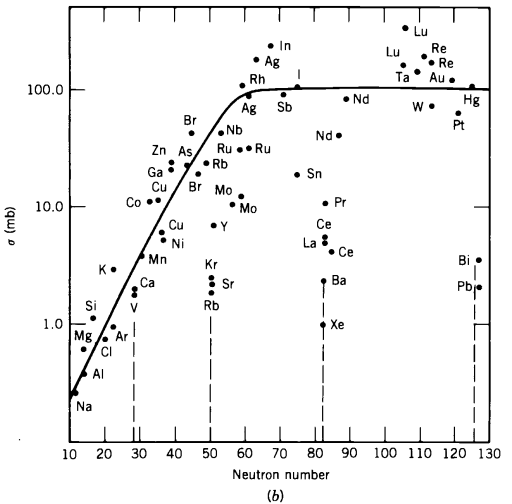
\includegraphics[width=\textwidth]{Diagramas Tema 5/Seccion eficaz vs neutrones.png}
        \captionof{figure}{Sección eficaz de captura neutrónica de varios núcleos.} 
    \label{fig: Seccion eficaz captura neutronica}
\end{center}
\end{minipage}
\hfill
\begin{minipage}{0.4\textwidth}
        \centering
    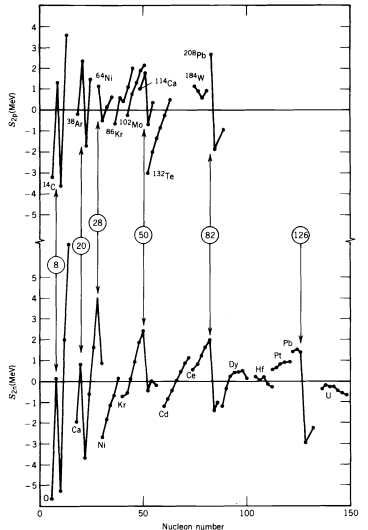
\includegraphics[width=\textwidth]{Diagramas Tema 5/Energias de separacion en funcion vs A.png}
    \captionof{figure}{(Arriba) Energías de separación de dos protones para secuencias de isótopos. Se indica el miembro de menor $Z$. (Abajo) Energías de separación de dos neutrones.}
    \label{fig: Energias de separacion}
\vfill
    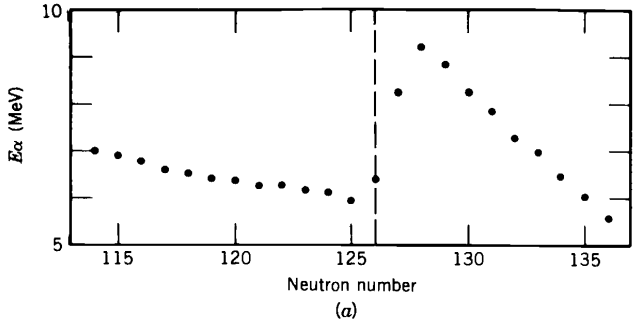
\includegraphics[width=\textwidth]{Diagramas Tema 5/Energia desintegracion alfa vs neutrones.png}
        \captionof{figure}{Energías de las partículas $\alpha$ emitidas por isótopos de Rn.} 
    \label{fig: Energias de alfa vs neutrones}
\vfill
    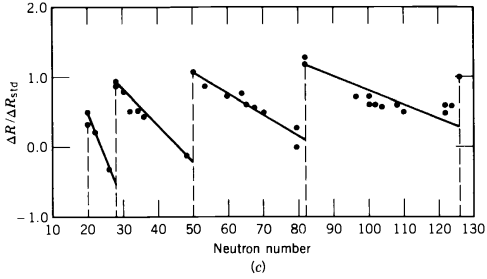
\includegraphics[width=\textwidth]{Diagramas Tema 5/Diferencias radio de carga equivalente.png}
        \captionof{figure}{Cambios en el radio de carga nuclear equivalente cuando tenemos $\Delta N=2$.} 
    \label{fig: Radios de carga nuclear equivalente y numeros magicos}
\end{minipage}
\newpage
\subsection{El potencial del modelo de capas}
A la hora de determinar el potencial que tiene el núcleo atómico, podemos pensar en distintos potenciales triviales para ver cómo reproducen los números de estados de ocupación
\subsubsection{Pozo esférico 3D}
\noindent
\begin{minipage}{0.6\textwidth}
El primer potencial que podemos probar es el pozo cuadrado partiendo de que la energía de ligadura por nucleón $\nicefrac{B}{A}\sim \mathrm{cte}$ y que la fuerza nuclear satura. Si suponemos un potencial con la forma 
\begin{equation*}
    V(r) \left \{ \begin{aligned}
        -&V_0 \quad r<R_0\\
        & 0 \ \, \quad r\geq R_0
    \end{aligned} \right.
\end{equation*}

Las soluciones en la componente radial del pozo cuadrado en 3 dimensiones corresponden a las funciones de Bessel, $$R_{nl}(r)= c\, j_l(\vec{k} \vec{r}) \quad \text{con} \quad k^2=\frac{2m}{\hbar^2}(E+V_0)$$ 
\end{minipage}
\hfill
\begin{minipage}{0.35\textwidth}
    \centering
    \includegraphics[width=\textwidth]{Diagramas Tema 5/PozoCuadrado3D.pdf}
    \captionof{figure}{Pozo cuadrado en 3 dimensiones.}
\end{minipage}
que si recordamos, para $l=0 \xrightarrow[]{} j_0=\dfrac{\sin(kr)}{kr}$, mientras que para $l \neq 0$ son más complicadas. 
\\\\
Una cosa que podemos hacer es tomar el pozo infinito, con la condición de que $j_l(kR_0)=0$, así las energías están relacionadas con los 0`s de las funciones de Bessel. \\\\
Las energías del pozo son $E_{nl}=(kr)_{nl}^2\dfrac{\hbar}{2mR^2_0}$ donde $(kr)_{nl}$ son los 0's de las funciones de Bessel; hemos de tener en cuenta también la degeneración que nos produce el spin.
En la siguiente tabla obtenemos los estados de ocupación del modelo.


\begin{table}[h]
\centering
\begin{tabular}{|ccccc|}
\hline
Estado & $(kr)_{nl}$ &                      & $2(2l+1)$ & Acumulado \\ \hline \hline
1s     & $3.142$       & (1)                  & 2         & \textcolor{applegreen}{2}         \\ \hline
1p     & $4.493$       & (2)                  & 6         & \textcolor{applegreen}{8}         \\ \hline
1d     & $5.763$       & \multirow{2}{*}{(3)} & 10        & 18        \\
2s     & $6.283$       &                      & 2         & \textcolor{applegreen}{20}        \\ \hline
1f     & $6.988$       & (4)                  & 14        & 34        \\ \hline
2p     & $7.725$       & \multirow{2}{*}{(5)} & 6         & 40        \\
1g     & $8.183$       &                      & 18        & \textcolor{red}{58}        \\ \hline
2d     & $9.095$       & \multirow{3}{*}{(6)} & 10        & 68        \\
1h     & $9.356$       &                      & 22        & 90        \\
3s     & $9.425$       &                      & 2         & \textcolor{red}{92}        \\ \hline
\end{tabular}
\caption{0's ordenados de las funciones de Bessel. Los números coloreados representan el número de estados de ocupación predichos por el modelo. Hemos utilizado la notación espectroscópica $nl$ donde $n$ es el $n$-ésimo 0 de cada una de las funciones y $l=0\equiv s, \ l=1\equiv p$... }
\label{tab: ceros de bessel}
\end{table}

Vemos que para los 3 primeros números mágicos el modelo sí que nos reproduce bien los resultados pero no para el resto.
\subsubsection{Oscilador armónico}
Como segunda idea podemos pensar que el potencial será una variación del oscilador armónico, en el que se van generando capas en las que la paridad va cambiando. Suponiendo un potencial con la forma
\begin{equation*}
    V(r)=\frac{1}{2}m\omega^2r^2
\end{equation*}
Las soluciones radiales de este potencial son los polinomios asociados de Laguerre
$$R_{nl}(r)=Nr^l \exp{\alpha r^2} L^{l+\nicefrac{1}{2}}_{\nicefrac{1}{2}(n-l)}(2\alpha r^2) \quad \text{con} \quad \alpha=\frac{m\omega}{2\hbar} \Rightarrow E_{nl}=\hbar \omega \qty(2n-l+\frac{3}{2})$$

Las energías están degeneradas $(2n+l+1)(2n+l+2)$ y aunque sí que sí que reproduce bien los tres primeros estados de ocupación, los niveles están equiespaciados, lo que no concuerda con los experimentos.

\begin{table}[h]
\centering
\begin{tabular}{|cccccc|}
\hline
$2n+l$             & Estado & l & n & $2(2l+1)$           & Acumulado                            \\ \hline \hline
2                  & 1s     & 0 & 1 & 2                   & \textcolor{applegreen}{2}            \\ \hline
3                  & 1p     & 1 & 1 & 6                   & \textcolor{applegreen}{8}            \\ \hline
\multirow{2}{*}{4} & 2s & 0 & 2 & \multirow{2}{*}{12} & \multirow{2}{*}{\textcolor{applegreen}{20}} \\
                   & 1d     & 2 & 1 &                     &                                      \\ \hline
\multirow{2}{*}{5} & 2p     & 1 & 2 & \multirow{2}{*}{20} & \multirow{2}{*}{\textcolor{red}{40}} \\
                   & 1f     & 3 & 1 &                     &                                      \\ \hline
\multirow{3}{*}{6} & 3s     & 0 & 3 & \multirow{3}{*}{30} & \multirow{3}{*}{\textcolor{red}{70}} \\
                   & 2d     & 2 & 2 &                     &                                      \\
                   & 1h     & 4 & 1 &                     &                                      \\ \hline
\multirow{3}{*}{7} & 3p & 1 & 3 & \multirow{3}{*}{42} & \multirow{3}{*}{\textcolor{red}{112}}       \\
                   & 2g     & 3 & 2 &                     &                                      \\
                   & 1i     & 5 & 1 &                     &                                      \\ \hline
\end{tabular}
\caption{Estados de ocupación y niveles orbitales de para el modelo de capas de oscilador armónico.}
\label{tab: ocupacion oscilador armonico}
\end{table}

Vemos que este potencial también reproduce bien los 3 primeros números de ocupación pero no el resto.\\\\
Una consecuencia de utilizar estos potenciales es que requieren que la energía de separación de los nucleones sea infinita y no incorporan nada de la corteza nuclear. El pozo infinito es demasiado abrupto mientras que el oscilador armónico es demasiado suave.\\\\
Necesitamos buscar un potencial más realista para alcanzar más números mágicos \newpage
\subsubsection{Potencial de Woods-Saxon}
\begin{minipage}{0.6\textwidth}
    Como ya hemos mencionado, el potencial no puede ser tan suave como el oscilador armónico ni tan brusco como el pozo infinito, buscaremos un punto intermedio que respete la distribución de carga y de materia nuclear. Este potencial es el potencial de \textbf{Woods-Saxon} y, salvo un signo, la forma que tiene la distribución de carga en un núcleo representado en la figura \ref{fig: Distribucion de carga nuclear}, y tiene la forma
\begin{equation}
    V(r)=-\dfrac{V_0}{1+\exp{\dfrac{r-R}{a}}}
    \label{eq: potencial de woods saxon}
\end{equation}
\end{minipage}
\hfill
\begin{minipage}{0.35\textwidth}
    \centering
    \includegraphics[width=\textwidth]{Diagramas Tema 5/PotencialWoodsSaxon.pdf}
    \captionof{figure}{Potencial de Woods-Saxon.}
    \label{fig: potencial woodssaxon}
\end{minipage}
\\\\
Este potencial satisface todas las propiedades del colectivas del núcleo descritas en el tema 3, en esencia lo que nos hace respecto al potencial del oscilador armónico es romper la degeneración de las capas principales. La rotura es tanto mayor, cuanto mayor es el momento angular orbital, por ejemplo: el orbital 1g ($l=4$) se mueve mucho y ocupa una posición intermedia entre las dos bandas anteriores generando un nuevo número mágico, el 58. Aun así no nos reproduce bien los números mágicos.\\\\
Como este potencial respeta las propiedades globales, vamos a modificarlo para que nos reproduzca bien los números mágicos. Fue en 1949 cuando María Goeppert Mayer y colaboradores quienes introdujeron una corrección que satisfacía los números mágicos. \\\\Esta corrección, al igual que el modelo de capas, nació de la física atómica. Si recordamos las correcciones de estructura fina, éstas se debían a correcciones relativistas, la distribución de carga del núcleo y al término de interacción \textbf{spin-órbita} producido por la interacción del momento magnético del electrón con el campo magnético generado por el mismo al girar alrededor del núcleo.
\\\\
La idea que ayudo a Mayer a entender esta modificación fue la dependencia fuerte del spin que hay en las fuerzas nucleares. El ejemplo estaba en el deuterón, un estado ligado de dos partículas distintas en un estado de spin 1, pero no ligado en el estado de spin 0 $$ \begin{aligned}
    &S=1 \xrightarrow[]{} {}^3S_1-{}^3D_1\quad \text{Deuterón}\\
    &S=0 \xrightarrow[]{} {}^1S_0 \quad \quad \quad \ \; \;\text{No ligado}
\end{aligned}$$ 
Debía de estar invertido pues el que tiene $j$ más alta tiene menor energía. Esto llevó a pensar que el potencial promedio debía tener un término de spin-órbita. Además como la interacción spin-spin era fuerte, la de spin-órbita también lo será, argumentemos esto algo más:
\begin{itemize}
    \item No puede ser de origen electromagnético, pues ha de modificar la estructura de capas del núcleo y esta interacción es demasiado débil como para cambiar las capas generadas por el potencial de Woods-Saxon.
    \item El signo es contrario al electromagnético, ya que para $j$ grandes tenemos menores energías.
    \item La dependencia radial dará la intensidad , y en princpio no tiene mucha influencia, por lo que parametrizaremos el modelo con $a$.
\end{itemize}

Vamos a construir el operador $V_\mathrm{SO}=a{\vec{l}\cdot \vec{s}}$, si partimos de la definición del momento angular total $\vec{J}=\vec{l}+\vec{s}$ obtenemos
\begin{equation*}
    \vec{j}^2=\qty(\vec{l}+\vec{s})^2=l^2+s^2+2\vec{l}\cdot \vec{s}\Rightarrow \vec{l}\cdot \vec{s}=\frac{1}{2}(j^2-l^2-s^2)
\end{equation*}
Así el valor esperado del operador $\vec{l}\cdot \vec{s}$ será
\begin{equation*}
\expval{\vec{l}\cdot \vec{s}}=\frac{\hbar^2}{2}\qty(j(j+1)-l(l-1)-s(s-1))
\end{equation*}
Si consideramos $s=\dfrac{1}{2}$ y $j=l\pm \dfrac{1}{2}$ obtenemos finalmente
\begin{equation}
    \expval{\vec{l}\cdot \vec{s}} = \left \{ \begin{aligned}
    &j=l+\frac{1}{2} \Rightarrow \frac{l}{2}\\
    &j=l+\frac{1}{2} \Rightarrow  -\frac{1}{2}(l+1)
\end{aligned}\right.
\label{eq: valor esperado operador spin orbita}
\end{equation}

La anchura de la degeneración, $\Delta w$, vendrá dada por 
\begin{equation*}
   \Delta w= \expval{\vec{l}\cdot \vec{s}}_{j=l+1/2}-\expval{\vec{l}\cdot \vec{s}}_{j=l-1/2}=\frac{\hbar}{2}(2l+1)
\end{equation*}

Por lo tanto, a medida que aumenta el momento angular orbital, mayor será la separación entre niveles. En las capas bajas no ocurre nada respecto a los $l$ bajos.\\\\ Si consideramos el nivel 1f, $l=3$, éste degenera en $j=l \pm \nicefrac{1}{2}=\nicefrac{5}{2},\nicefrac{7}{2}$, con estados de ocupación 6 y 8 respectivamente. La degeneración para cada nivel es $(2j+1)$, producto de los valores $m_j$.\\\\
Por último hemos de considerar que $V_\mathrm{SO}<0$, así los miembros con mayor $j$ son arrastrados hacia niveles menos energéticos, lo que nos genera los \textbf{números mágicos}, el modelo además predice un nuevo número mágico, el 184.\\\\ 
La intensidad $a$ del potencial la podemos predecir de datos experimentales, para ello podemos coger dos núcleos con la misma $l$, pero con distinta $j$. La diferencia de energías se deberá al $V_\mathrm{SO}$, siendo $a=\dfrac{2\Delta w}{2l+1}$, si, por ejemplo, escogemos los núcleos de oxígeno-16 y calcio-40, obtenemos que $a=\unit[-2.03]{MeV^{-1}s^{-2}}$ y $a=\unit[-2.05]{MeV^{-1}s^{-2}}$ respectivamente. \\\\
En la siguiente página vemos como se desdoblan los niveles de energías para protones y neutrones. Las discrepancias entre protones y neutrones de la figura vienen dadas por las contribuciones coulombianas de la repulsión entre protones.
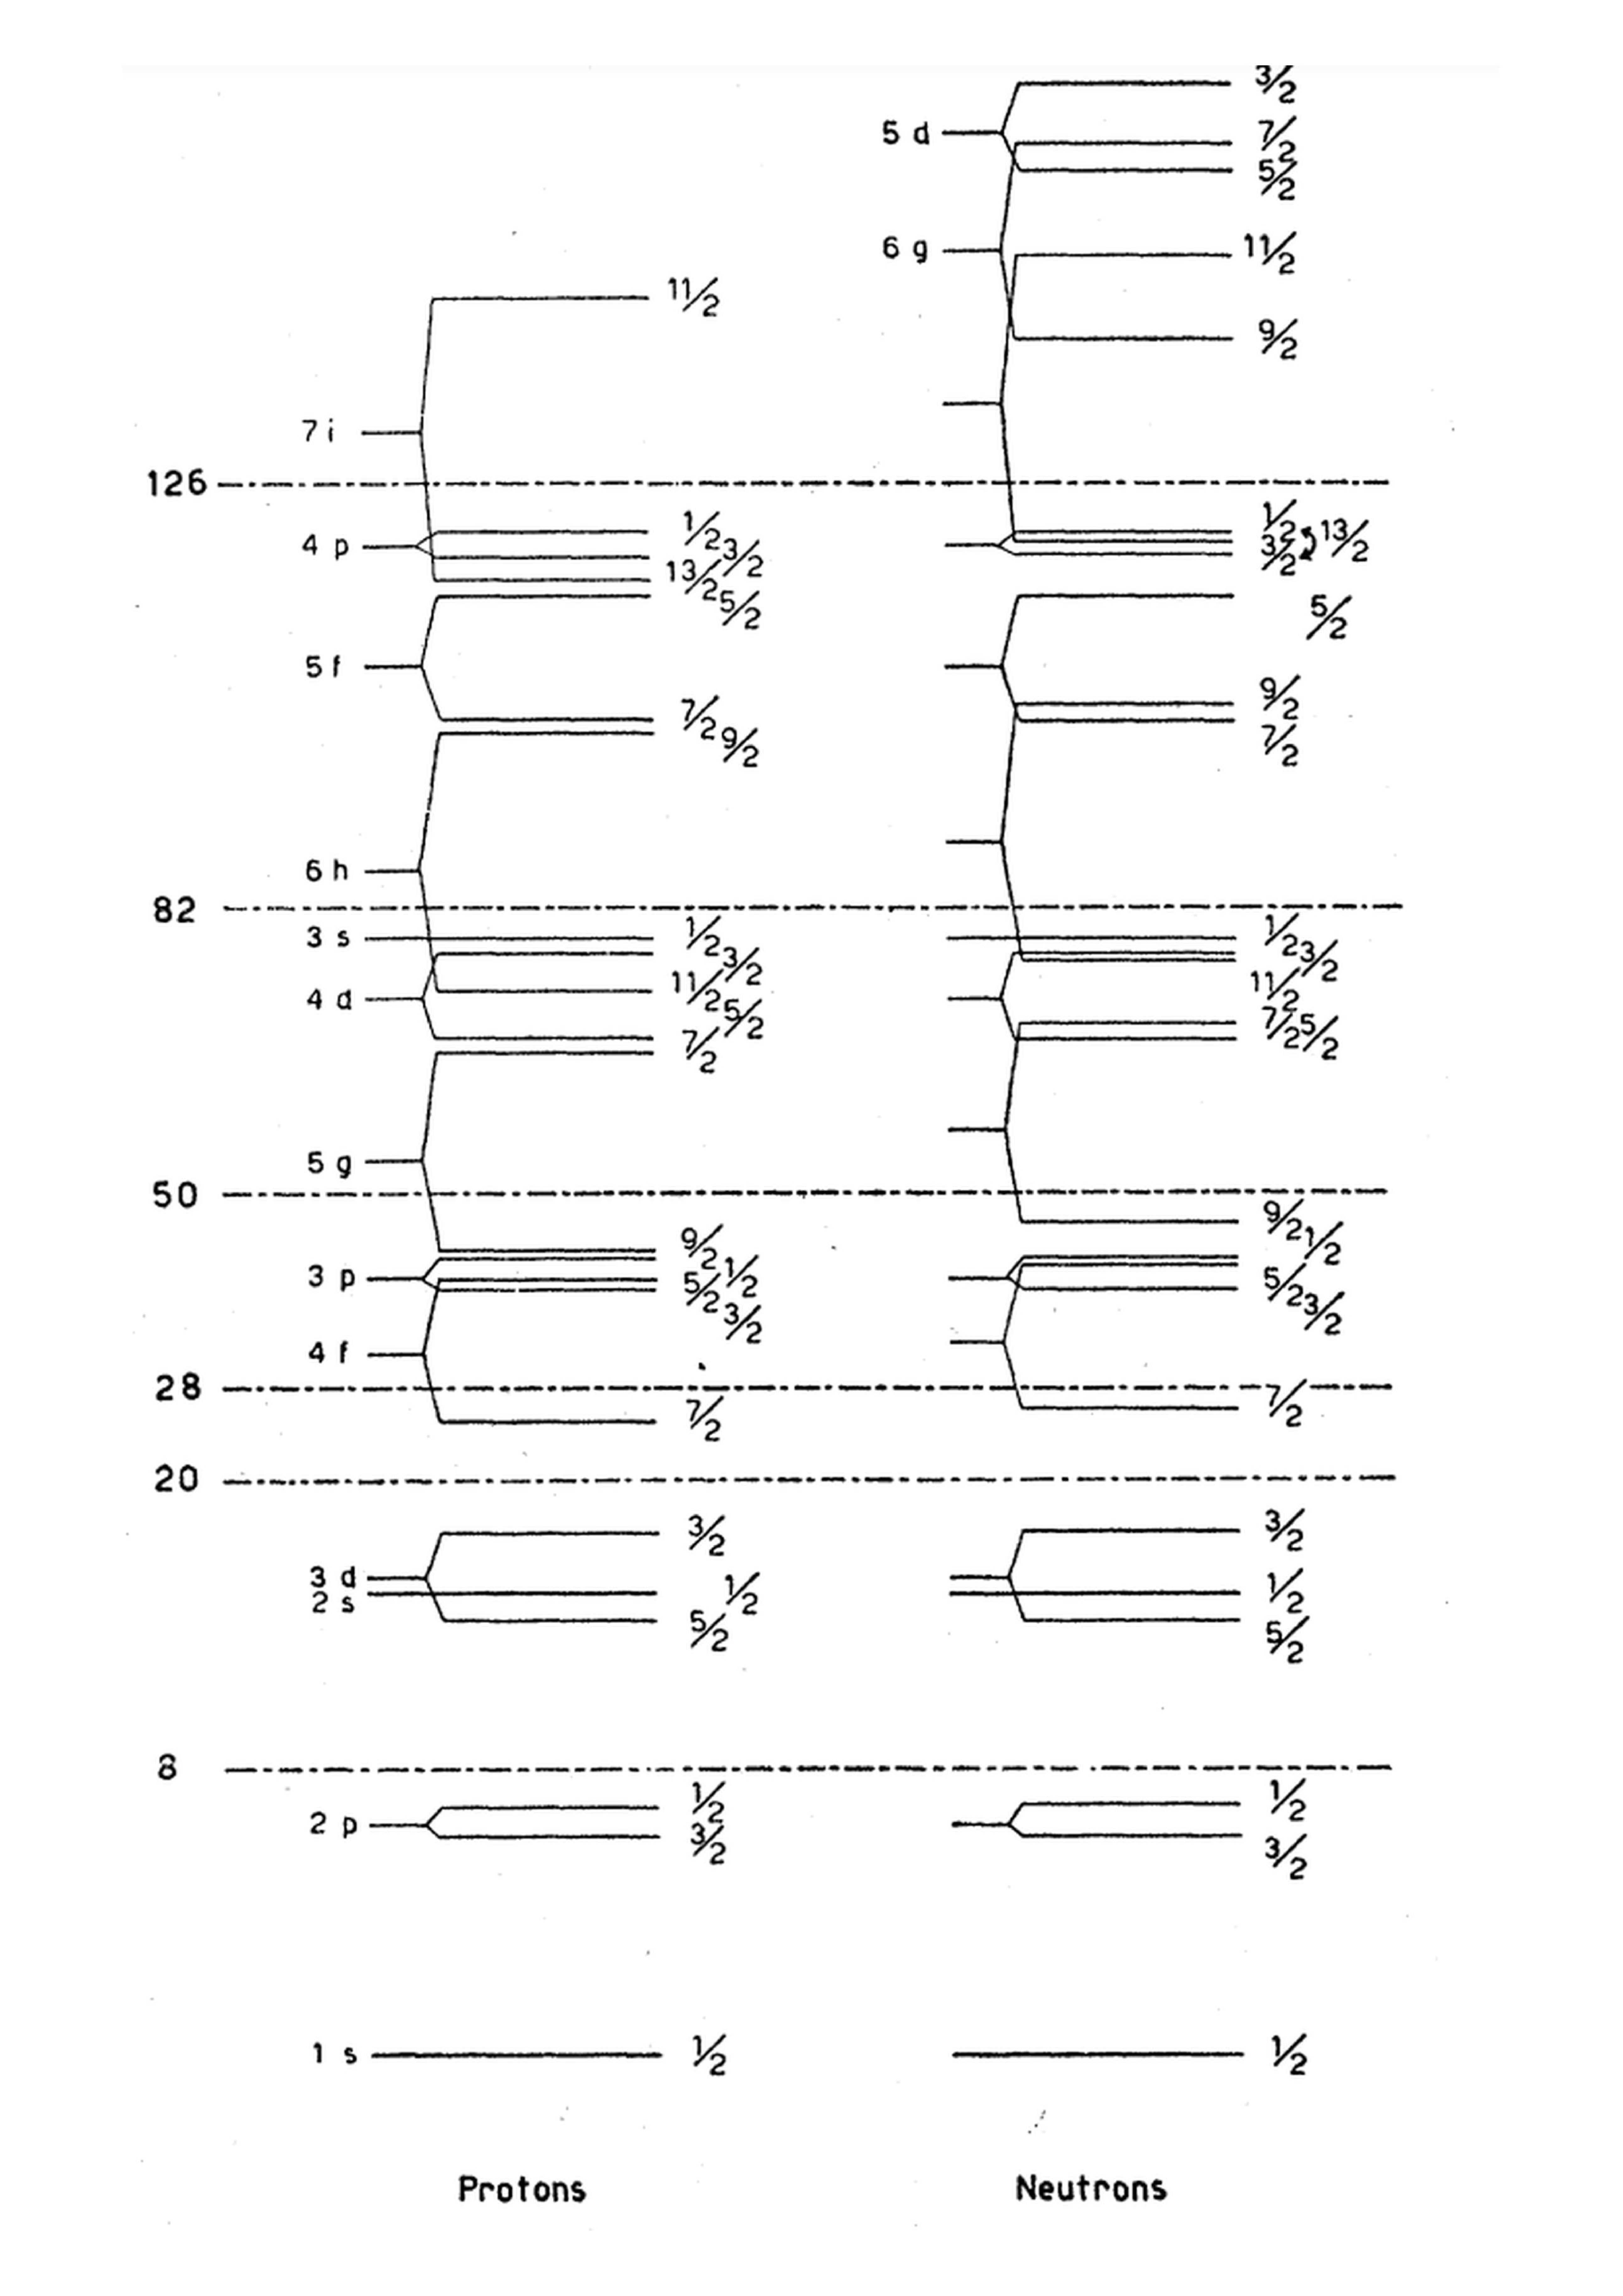
\includepdf[pages=1]{Diagramas Tema 5/Niveles energia modelo de capas.pdf}

\section{Predicciones del modelo de capas. Regla de Nordheim}
Para determinar la $J^P$ de los núcleos a partir del modelo de capas utilizaremos el \textbf{modelo extremo de partícula independiente}. la secuencia de niveles del modelo de capas se va llenando por orden creciente de energía. En el modelo de partícula independiente las propiedades del núcleo vienen determinadas únicamente por el nucleón desapareado, por lo tanto
\begin{equation*}
    J=j \quad \text{donde} \quad P=(-)^l, l=j\pm \frac{1}{2}
\end{equation*}

por lo que el momento angular orbital fija el valor de la paridad del núcleo. \\\\
Este modelo funciona muy bien cerca de la capa cerrada y falla para $A<150$ y $190<A<220$, que en esencia son núcleos muy poco esféricamente simétricos.\\\\
Lejos de capa cerrada el nucleón desapareado también determina las propiedades del núcleo, pero las fuerzas residuales no incluidas en el potencial central efectivo producen fuerzas de emparejamiento muy intensas que modifican los niveles energéticos y acoplan nucleones por pares a $J^P=0^+$
\begin{tcolorbox}[colback=airforceblue!20, colframe=airforceblue, title={Ejemplo: $J^P$ de los isótopos $^{15}\mathrm{O}$ y $^{17}\mathrm{O}$}]
    Experimentalmente medimos que $J^P\qty(^{15}_8\mathrm{O}_7)=\nicefrac{1}{2}^-$ y $J^P\qty(^{17}_8\mathrm{O}_9)=\nicefrac{5}{2}^+$, utilizando el modelo de capas tenemos 
    $$\begin{aligned}
        &^{15}_8\mathrm{O}_7 \xrightarrow[]{} 1p_{\nicefrac{1}{2}} \left \{ \begin{aligned}
            &l=1 \Rightarrow P=-\\
            &j=\nicefrac{1}{2}
        \end{aligned} \right. \Rightarrow J^P=\frac{1}{2}^-\\
        &^{17}_8\mathrm{O}_9 \xrightarrow[]{} 1d_{\nicefrac{5}{2}} \left \{ \begin{aligned}
        &l=2 \Rightarrow P=+ \\
            &j=\nicefrac{5}{2}
        \end{aligned} \right. \Rightarrow J^P=\frac{5}{2}^+
    \end{aligned}$$

    El modelo de capas extremo de partícula independiente es capaz de predecir correctamente la $J^P$ de la mayor parte de los estados fundamentales de los estados con $A$ impar.
\end{tcolorbox}
\subsection{Regla de Nordheim}

EL modelo de capas se  puede utilizar también para obtener información acerca del spin del estado fundamental de núcleos impar-impar. Para eso se utiliza la regla de Nordheim. Llamemos $j_p$ y $l_p$ al spin y al momento angular orbital del protón desapareado y $j_n$ y $j_n$ a los del neutrón desapareado. Así, definimos al número de Nordheim como
\begin{equation}
    N_\mathrm{Nord}=j_p-l_p+j_n-l_n
    \label{eq: numero de nordheim}
\end{equation}

La paridad del núcleo vendrá dada por $P=(-)^{l_n}(-)^{l_p}$. La regla de Nordheim dice 
\begin{itemize}
    \item Si $N_\mathrm{Nord}=0 \Rightarrow J=\abs{j_n-j_p}$, por lo que el spin del protón y del neutrón están antiparalelos y por tanto el núcleo va a intentar poner arriba el neutrón.
    \item Si $N_\mathrm{Nord}=\pm 1 \Rightarrow J=\abs{j_n-j_p}$ ó $j_n+j_p$ en este caso los spines ya son paralelos.
\end{itemize}

La regla de Nordheim, aplicable a núcleos con más de un nucleón fuera de capas cerradas, fue confirmada de forma teórica por De Shalit y Walecka.

\section{Momento dipolar magnético. Líneas de Schmidt}
El modelo de partícula independiente predice que el momento dipolar magnético de un núcleo con $A$ impar es debido exclusivamente al nucleón desapareado. El momento dipolar magnético en unidades del magnetón nuclear es (ecuación \ref{eq: momento magnetico})
\begin{equation}
    \frac{\vec{\mu}}{\mu_N}=\sum_{i=1}^A \qty(g_i^{(l)}\vec{l}_i+g_i^{(s)}\vec{s}_i) \Rightarrow \frac{\vec{\mu}}{\mu_N}=g_j^{(l)}\vec{l}_j+g_j^{(s)}\vec{s}_j
    \label{eq: momento dipolar nucleon desapareado}
\end{equation}

Por definición, sabemos que el valor esperado del momento magnético en el estado de máxima proyección es 
$$\begin{aligned}
    &\mel{jj}{\vec{\mu}}{jj}=\mel{jj}{g^{(l)}\vec{l}+g^{(s)}\vec{s}}{jj}=\mel{jj}{g^{(l)}l\textcolor{red}{+g^{(l)}s-g^{(l)}s}+g^{(s)}s}{jj}=\\&g^{(l)}\mel{jj}{j}{jj}+ \qty(g^{(s)}-g^{(l)}) \mel{jj}{s}{jj}=g^{(l)}j+\qty(g^{(s)}-g^{(l)})\qty(\pm j\frac{1}{2j+1})
\end{aligned}$$
Por lo que la ecuación \ref{eq: momento dipolar nucleon desapareado} será
\begin{equation}
    \frac{\vec{\mu}}{\mu_N}=\qty(g^{(l)}+\qty(g^{(s)}-g^{(l)})\qty(\pm \frac{1}{2l+1}))j
    \label{eq: resultado momento dipolar magnetico nucleon desapareado}
\end{equation}

Donde hemos utilizado el Teorema de Proyección\footnote{Tenemos que $$\expval{s}=\frac{\expval{\vec{s}\cdot \vec{j}}}{\expval{j^2}}\expval{j}, \quad \expval{\vec{s}\cdot \vec{j}}=\frac{1}{2}\qty(\expval{j^2}-\expval{s^2}-\expval{l^2})=\frac{\hbar^2}{2}\qty(j(j+1)+\frac{3}{4}-l(l+1))$$ como $j=l\pm \nicefrac{1}{2}$, $$\expval{s}=\left \{ \begin{aligned}
    &j=l+\frac{1}{2}\Rightarrow \frac{j}{2l+1}\\
    &j=l-\frac{1}{2}\Rightarrow -\frac{j}{2l+1}
\end{aligned} \right.$$} para obtener este resultado.\\\\
Vamos a recordar que las razones giromagéticas de los nucleones son $$
g_i^{(l)}= \left \{\begin{aligned}
    &g_p^{(l)}=1 \\
        &g_n^{(l)}=0
    \end{aligned} \right. \quad \quad \quad g_i^{(s)}= \left \{\begin{aligned}
        &g_p^{(s)}=5.58 \\
        &g_n^{(s)}=-3.82 \end{aligned} \right.$$
\newpage
\noindent

\subsection{Líneas de Schmidt}
En las siguientes figuras hemos representado los valores calculados como líneas sólidas, conocidas como \textbf{líneas de Schmidt}; realizado por él mismo en 1937.  Los valores experimentales caen con los límites de las líneas de Schmidt, pero normalmente tienen valores menores y presentan más dispersión.
\\\\ Una posible mejora se produce por asumir que el valor de las razones giromagnéticas de los nucleones libres y de los nucleones en el núcleo no tienen porqué ser iguales. Para núcleos ligeros el acuerdo entre modelo y experimento es bastante satisfactorio.

\begin{figure}[h!]
    \centering
    % Subfigura para protones impares
    \begin{subfigure}[b]{0.45\textwidth}
        \centering
        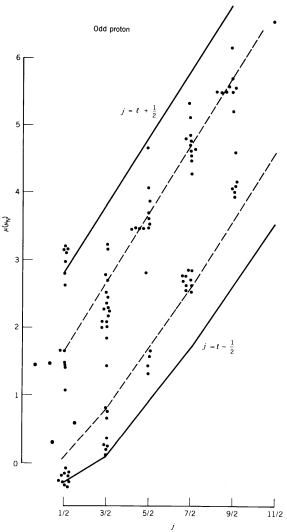
\includegraphics[width=\textwidth]{Diagramas Tema 5/Lineas de Schmidt protones impares.png}
        \caption{Líneas de Schmidt para protones impares.}
        \label{fig:lineas-schmidt-protones}
    \end{subfigure}
    \hfill
    % Subfigura para neutrones impares
    \begin{subfigure}[b]{0.45\textwidth}
        \centering
        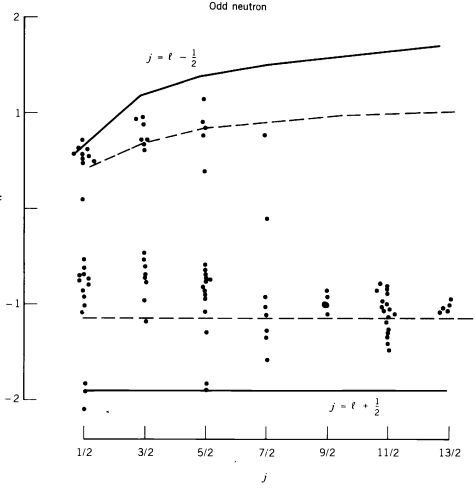
\includegraphics[width=\textwidth]{Diagramas Tema 5/Lineas de Schmidt neutrones impares.png}
        \caption{Líneas de Schmidt para neutrones impares.}
        \label{fig:lineas-schmidt-neutrones}
    \end{subfigure}
    \caption{Líneas de Schmidt para nucleones impares.}
    \label{fig:lineas-schmidt-nucleones}
\end{figure}

\part{Apéndices}
\appendix
\pagestyle{fancy}
\fancyhead[R]{Física Nuclear y de Partículas: Apéndice A}
\fancyhead[L]{4º Grado en Física}
\chapter{Probabilidad de transición en teoría de perturbaciones}
\label{chap: Apendice A}
En teoría de perturbaciones dependiente del tiempo, consideramos transiciones (ya sea en colisiones o en desintegraciones) del estado inicial de un sistema, que denotamos por $\Psi$, a un conjunto de estados finales como resultado de una acción de una perturbación, que denotamos por $V(H')$.\\\\
Nuestro sistema para tiempos $t<0$ viene descrito por un hamiltoniano $H_0$. El sistema está en un estado estacionario de energía $E_m$, que es uno de los autoestados de $H_0$. Por lo tanto 
\begin{equation}
    \Psi(0)=\phi_m \exp{-i \frac{E_mt}{\hbar}}
    \label{eq: estado estacionario}
\end{equation}

Para $t>0$ comienza a actuar la perturbación y se describe con $H=H_0+V(H')$. Eso da lugar a transiciones a otros estados del sistema $\phi_n$. Por lo tanto
\begin{equation}
    \Psi (t)=\sum^\infty _{n=0} c_n(t) \phi_n \exp{-i \frac{E_nt}{\hbar}}
    \label{eq: ecuacion de onda con perturbacion}
\end{equation}
donde las funciones $\phi_n$ son un conjunto completo de autofunciones ortonormales de $H_0$, es decir
\begin{equation}
    H_0\phi_n=E_n\phi_n
    \label{eq: ecuacion de sch independiente del tiempo}
\end{equation}
Por tanto, $c_n(0)=1$ para $n=m$ y cero para los demás valores de $n$. La función de onda de la ecuación \ref{eq: estado estacionario} ha de satisfacer la ecuación de Schrödinger dependiente del tiempo
\begin{equation}
    H\Psi(t)=i\hbar \pdv{\Psi(t)}{t}
    \label{eq: ecuacion de sch dependiente del tiempo}
\end{equation}
Si sustituimos \ref{eq: ecuacion de onda con perturbacion} en \ref{eq: ecuacion de sch dependiente del tiempo}
\begin{equation}
    i\hbar \sum^\infty _{n=0} \qty(\dv{c_n(t)}{t}) \phi_n \exp{-i \frac{E_nt}{\hbar}} =\sum^\infty _{n=0} Vc_n(t) \phi_n \exp{-i \frac{E_nt}{\hbar}}
    \label{eq: desarrollo ESDT 1}
\end{equation}
Multiplicando por $\phi_k^*$ la ecuación \ref{eq: desarrollo ESDT 1} y usando la ortonormalidad $\bra{\phi_k}\ket{\phi_n}=\delta_{kn}$ obtenemos
\begin{equation}
   i\hbar \dv{c_k(t)}{t}= \sum^\infty _{n=0} c_n(t) M_{nk} \exp{-i \frac{E_nt}{\hbar}} \quad \text{siendo} \quad M_{nk}=\int \phi_k^* V \phi_n \dd V
\end{equation}

En teoría de perturbaciones a primer orden la perturbación se supone que es débil y las probabilidades de transición lo suficientemente pequeñas para que durante el tiempo considerado $c_m(t)=1$ y $c_n(t)\simeq 0$ si $n\neq m$. Así, suponiendo que $V$ es constante para $t>0$ e integrando en el tiempo 
\begin{equation}
\begin{aligned}
        c_k(t)=& \frac{-i}{\hbar} \int^t_0 M_{mk} \exp{-i \frac{\qty(E_m-E_k)t}{\hbar}}\dd t=
        \left. \frac{-i}{\hbar} M_{mk} \frac{\hbar}{-i (E_m-E_k)}  \exp{-i \frac{\qty(E_m-E_k)t}{\hbar}}\right |^t_0= \\ &=M_{mk} \exp{-i \frac{\qty(E_m-E_k)}{2\hbar}t} 2i \frac{\sin(\dfrac{E_m-E_k}{\hbar}t)}{E_m-E_k}
\end{aligned}
\end{equation}
La probabilidad de transición por unuidad de tiempo a todos los estados será 
\begin{equation}
    W=\frac{1}{t} \sum_n \abs{c_n(t)}^2=\frac{1}{t} \int^\infty_\infty \abs{c_n(t)}^2 \qty(\dv{N}{E_n}) \dd E_n
    \label{eq: Probabilidad de transicion por unidad de tiempo}
\end{equation}
La primera igualdad representa un conjunto discreto de estados mientras que la segunda representa un conjunto de estados muy próximos entre sí que es lo que ocurre en procesos de colisiones o desintegraciones. $\dfrac{\dd N}{\dd E_n}$ es la densidad de estados por intervalo de energía. Si definimos 
\begin{equation}
    x=\frac{E_k-E_m}{2\hbar}t
\end{equation}
Entonces 
\begin{equation}
    W=\frac{1}{t} 4\abs{M_{mk}}^2 \int^\infty_\infty \frac{t^2}{4\hbar^2} \frac{\sin^2{x}}{x^2} \frac{2\hbar}{t} \dd x=\frac{2}{\hbar} \int^\infty_\infty \qty(\dv{N}{E}) \frac{\sin^2{x}}{x^2} \dd x
\end{equation}
La función $\dfrac{\sin^2{x}}{x^2}$ tiene un máximo para $x=0$ i.e $E_k=E_m$ y el primer cero es en $x=\pm \pi$. La contribución a la intergal más allá de $x=\pm \pi$ es pequeña $\sim 10\%$. El correspondiente intervalo de energía es $\dd E_k=\dfrac{2\pi \hbar}{t} \sim \unit[4 \cdot 10^{-15}]{eV}$ para $t=\unit[1]{s}$. Esto se debe a que la energía se debe conservar dentro de los límites del principio de incertidumbre, $E_k \approx E_m$. Por tanto, la densidad de estados se puede considerar constante sobre el intervbalo $\dd E_n$ y usando que $$\int^\infty_\infty \frac{\sin^2{x}}{x^2} \dd x =\pi $$ se obtiene 
\begin{equation}
    W=\frac{2\pi}{\hbar} \abs{M_\text{if}}^2 \dv{N}{E_\text{f}} \quad \text{con} \quad M_\text{if}=\bra{\phi_\text{f}}V\ket{\phi_\text{i}}
    \label{eq: regla de oro de fermi}
\end{equation}
Es decir, el elemento de matriz en la transición de un estado inicial $i$ a un conjunto de estados finales $f$. $\phi_i$ y $\phi_f$  corresponde a la parte espacial de las funciones de onda. A la densidad de estados finales se les suele denotar como $\dfrac{\dd N}{\dd E_\text{f}}=\rho_\text{f}$ y se denomina espacio fásico. Esta expresión se conoce como la \textbf{regla de oro de Fermi} de la mecánica cuántica no relativista.\\\\
Aunque la deducción de la regla de oro la hemos hecho para teoría de perturbaciones, el resultado es también válido para el caso general.


\pagestyle{fancy}
\fancyhead[R]{Física Nuclear y de Partículas: Apéndice B}
\fancyhead[L]{4º Grado en Física}
\chapter{Detección de partículas. Secciones eficaces y anchuras de desintegración}
\label{chap: Apendice B}
La mayor parte de la información sobre las propiedades de las partículas y sus interacciones viene de datos experimentales de secciones eficaces de colisión y probabilidades (anchuras) de desintegración.\\\\
Consideramos un ejemplo de una colisión
\begin{equation}
    a+b \longrightarrow c+d
    \label{eq: colision}
\end{equation}
Si denotamos como $b$ al blanco y $a$ al proyectil, entonces la \textbf{sección eficaz} de la reacción \ref{eq: colision} se defina como la probabilidad de transición $W$ por unidad de flujo incidente y de partícula en el blanco. Si denotamos $n_a$ a la densidad de partículas del haz incidente y $v_i$ a la velocidad relativa entre los proyectiles y el blanco, entonces el flujo de partículas por unidad de tiempo a trabés de la unidad de área perpendicular al haz será
\begin{equation}
    \phi=n_a v_i
\end{equation}
Si el blanco contiene $n_b$ partículas por unidad de área, todas con la misma sección eficaz efectiva $\sigma$, para que ocurra la reacción \ref{eq: colision}, la probabiliad de que cualquier partícula incidente golpee un blanco es $\sigma n_b$. La probabilidad de transición por cada partícula blanco será entonces
\begin{equation}
    W=\sigma \phi=\sigma \frac{N_a}{V} v_i \quad \text{con} \quad n_a=\frac{N_a}{V}
    \label{eq: Probabilidad de transicion para cada particula blanco}
\end{equation}
Considerando una partícula en el volumen de normalización, $N_a=1$, entonces 
\begin{equation}
    \sigma=\frac{V}{v_i}W \quad \text{con} \quad W=\frac{2\pi}{\hbar} \abs{M_\text{if}}^2\rho_\text{f}
    \label{eq: seccion eficaz}
\end{equation}
La expresión de $W$ es igualmente válida para procesos de desintegración en las que el estado incial es una partícula que se destruya en un estado final
\begin{equation}
    X\longrightarrow c+d
    \label{eq: desintegracion}
\end{equation}
En este caso no se necesita haz para generar la reacción, y por tanto la probabilidad de transición para cada partícula inestable será
\begin{equation}
    W=\lambda
    \label{eq: constante de desintegracion}
\end{equation}
donde $\lambda$ se denomina \textbf{constante de desintegración}.\\\\
En este caso 
\begin{equation}
    \Gamma=\lambda \hbar= 2\pi \abs{M_\text{if}}^2 \rho_\text{f}
    \label{eq: anchura de desintegracion}
\end{equation}
se denomina a \textbf{anchura de desintegración}, como ya vimos en el capítulo 1
\begin{tcolorbox}[colback=applegreen!20, colframe=applegreen, title={Análisis dimensional: Sección eficaz, constante y anchura de desintegración}]
\begin{equation*}
\begin{aligned}
        \qty[\sigma]\equiv \frac{L^3}{LT} \frac{1}{ET} E^2 \frac{1}{L}\equiv L^2 \hspace{1.5cm}
        \qty[\Gamma]\equiv E^2\frac{1}{E}\equiv E \hspace{1.5cm}
        \qty[\lambda]\equiv \frac{1}{ET}E^2 \frac{1}{E}\equiv T^{-1}
\end{aligned}
\end{equation*}
La unidad habitual en la que se suele medir la sección eficaz en física de partículas es el $\unit{barn}\equiv \unit[10^{-28}]{m^2}$ que es del orden de la superficie de un núcleo.

\begin{equation*}
        \qty[\sigma]\equiv \frac{1}{E^4T^4}L^6E^2 \frac{E^2T^2}{L^2} \frac{T}{L} \frac{T}{L}\equiv L^2 
\end{equation*}
Obteniendo de nuevo que es una superficie.
\end{tcolorbox}

En ambos casos, colisión o desintegración, la expresión de $M_\text{if}=\bra{\Psi_\text{f}}H'\ket{\Psi_\text{i}}$, se obtuvo bajo la hipótesis de que $H'\equiv V\ll H_0$, siendo $H_0$ el hamiltoniano sin perturbar. Si $H'$ no fuese una perturbación, $M_\text{if}$ no se puede calcular de manera explícita y la expresión de $W$ se toma como una definición de $M_\text{if}$. En estos casos los datos de secciones eficaces y anchuras de desintegración se usan para determinar el elemento de matriz de transición $M_\text{if}$.
\section{Densidad de estados finales. Casos de interés}
La densidad de estados finales dependerá del número de partículas en el estado final y su carácter relativista o no relativista. Posteriormente analizaremos distintas situaciones, de momento nos ceñimos al proceso \ref{eq: colision}. Denotemos por $E_0$ la energía total en el centro de masas (CM).
\begin{equation}
    E_0=\sqrt{p_\text{f}^2c^2+m_c^2c^4}+\sqrt{p_\text{f}^2c^2+m_d^2c^4} \quad \text{con} \quad \abs{p_c}=\abs{p_d}=p_\text{f}
    \label{eq: energia total en el CM colision}
\end{equation}
\noindent
\begin{minipage}{0.6\textwidth}
Necesitamos conocer el número de estados accesibles con momento entre $p_\text{f}$ y $p_\text{f}+\dd p_\text{f}$ en el ángulo sólido subtendido por el detector $\dd \Omega$. Se trata de la intersección del volumen de un casquete esférico de radio $p_\text{f}$ con el ángulo sólido $\dd \Omega$, es decir $$\dd \Omega\, p_\text{f}^2 \,\dd p_\text{f}$$
\end{minipage}
\hfill
\begin{minipage}{0.35\textwidth}
    \centering
    \includegraphics[]{Diagramas Apendices/B_AnguloSolido.pdf}
    \captionof{figure}{Definición de ángulo sólido.}
\end{minipage}\newpage
El número de estados dependerá del volumen mínimo de la celda unidad. Al trabajar con ondas planas tomamos cajas de lado $L$ y ponemos condiciones de periodicidad, dando lugar a la cuantización del momento lineal,
\begin{equation}
    p_i=n_i2\pi\frac{\hbar}{L} \quad \text{con} \quad n_i=1,2,3...
\end{equation}
Por tanto el volumen de la celda unidad mínima será 
\begin{equation}
    p_xp_yp_X=\frac{h^3}{L^3}=\frac{h^3}{V}
\end{equation}
y por lo tanto la densidad de estados en el estado final será
\begin{equation}
\rho_\mathrm{f}=\dv{N}{E_0}=\dd \Omega\, p_\mathrm{f}^2 \frac{V}{h^3} \dv{p_\mathrm{f}}{E_0} g_\mathrm{f}
\end{equation}
Siendo $g_\mathrm{f}$ un factor que depende del spin (degeneración). Si integramos a todos los ángulos de los productos de la reacción, la integral del ángulo sólido es $4\pi$, entonces
\begin{equation}
    \rho_\mathrm{f}= 4\pi  p_\mathrm{f}^2 \frac{V}{h^3} \dv{p_\mathrm{f}}{E_0} g_\mathrm{f}
\end{equation}
y por tanto
\begin{equation}
    \sigma=\frac{1}{\pi \hbar^4} V^2 \abs{M_\mathrm{if}}^2 \frac{p_\mathrm{f}^2}{v_i} \dv{p_\mathrm{f}}{E_0}g_\mathrm{f}
    \label{eq: seccion eficaz estado final}
\end{equation}

\begin{tcolorbox}[colback=applegreen!20, colframe=applegreen, title={Análisis dimensional: Sección eficaz del estado final}]
\begin{equation*}
        \qty[\sigma]\equiv \frac{1}{E^4T^4}L^6E^2 \frac{E^2T^2}{L^2} \frac{T}{L} \frac{T}{L}\equiv L^2 
\end{equation*}
Obteniendo de nuevo que es una superficie.
\end{tcolorbox}
\subsubsection{Sobre el factor $V^2\abs{M_\mathrm{if}}^2$}
En los textos no suele aparecer el factor de volumen ya que se trabaja con volumen unidad. Ese factor cancela con la normalización de las ondas planas en $M_\mathrm{if}=\dfrac{1}{\sqrt{V}} \bra{\phi_\text{f}}V\ket{\phi_\text{i}} \dfrac{1}{\sqrt{V}}$. Por tanto, se puede escribir simplemente $\abs{M_\mathrm{if}}^2$, siendo consciente de sus dimensiones.\\\\
Vamos ahora a proceder al cálculo explícito de la densidad de estados finales en casos partículares de interés. Este cálculo es tanto aplicable a colisiones como desintegraicones. Analizaremos casos de las partículas en el estado final y un caso con tres partículas.
\newpage
\subsection{Dos partículas en el estado final. $B$ y $C$ relativistas}
\noindent Tenemos la desintegración $$A\longrightarrow B+C$$ la densidad de estados en la energía del estado final es
\begin{equation}
    \rho_\mathrm{f}=4\pi V\frac{p_\mathrm{f}^2}{\qty(2\pi \hbar)^3} \dv{p_\mathrm{f}}{E_0}
\end{equation}
Siendo $E_0=m_Ac^2=\sqrt{p^2_\mathrm{f}c^2+m_B^2c^4}+\sqrt{p^2_\mathrm{f}c^2+m_C^2c^4}$ la energía de la partícula $A$ en reposo. Derivando respecto de $p_\mathrm{f}$ obtenemos$$\dv{E_0}{p_\mathrm{f}}=\frac{p_\mathrm{f}c^2E_0}{E_BE_C}$$
Por lo tanto la densidad de estados será
\begin{equation}
\rho_\mathrm{f}=4\pi V\frac{p_\mathrm{f}^2}{\qty(2\pi \hbar)^3} \frac{E_BE_C}{p_\mathrm{f}c^2E_0}=\frac{V p_\mathrm{f}c}{2\pi^2\qty(\hbar c)^3}  \frac{\qty(E_0-E_c)E_c}{E_0}
    \label{eq: densidad de estados final desintegracion relativista}
\end{equation}
\subsection{Dos partículas en el estado final. $B$ y $C$ no relativistas}
\noindent La desintegración $\alpha$ \footnote{En el límite $m_C\sim 0$ en lugar de ser una desintegración $\alpha$ es una desintegración electromagnética.} de los núcleos pesados es un ejemplo de este tipo de escenario. Tenemos la desintegración $$A\longrightarrow B+C$$ Supongamos que $T=\qty(m_A-m_B-m_C)c^2\ll m_Bc^2,m_Cc^2$ entonces
\begin{equation*}
E_0=m_Ac^2=m_Bc^2+\frac{p_\mathrm{f}^2}{2m_B}+\frac{p_\mathrm{f}^2}{2m_C} \Rightarrow T=\frac{p_\mathrm{f}^2}{2}\qty(\frac{1}{m_B}+\frac{1}{m_C})=\frac{p_\mathrm{f}^2}{2}\frac{m_B+m_C}{m_Bm_C}=\frac{p_\mathrm{f}^2}{2\mu}
\end{equation*}
Obteniendo que el momento en el estado final ha de ser $    p_\mathrm{f}=\qty(2\mu T)^{1/2}$. Derivando la energía del sistema respecto al momento en el estado final obtenemos
\begin{equation}
    \dv{E_0}{p_\mathrm{f}}=\frac{p_\mathrm{f}}{\mu}
\end{equation}
Así la densidad de estados en el estado final será
\begin{equation}
    \rho_\mathrm{f}= \frac{2\pi V T^{1/2}}{\qty(2\pi\hbar c)^3}\qty(2\mu c^2)^{3/2}
    \label{eq: densidad de estados final desintegracion no relativista}
\end{equation}

\subsection{Dos partículas en el estado final. $B$ y $C$ una partícula pesada y una relativista}
Supongamos que $T=\Delta M c^2=\qty(m_A-m_B-m_C)c^2$ y que $m_C\ll m_B$.
\begin{equation}
    E_0=m_Ac^2= m_Bc^2+\cancelto{0}{\frac{p_\mathrm{f}^2}{2m_B}}+\sqrt{m_C^2c^4+p_\mathrm{f}^2c^2}
\end{equation}
Al ser una desintegración a dos cuerpos, el momento ha de ser el mismo para ambas partículas pero la energía cinética se la lleva casi en su totalidad la partícula ligera, por eso podemos despreciar el término de la energía cinética de la partícula $B$.
\\\\
De la expresión del momento final
\begin{equation}
    p_\mathrm{f}=\frac{1}{c}\qty{\qty[(m_A-m_B)c^2]^2-m_C^2c^4}^{1/2} \Rightarrow \dv{E_0}{p_\mathrm{f}}=\frac{p_\mathrm{f}c^2}{\sqrt{m_C^2c^4+p_\mathrm{f}^2c^2}}=\frac{p_\mathrm{f}}{m_A-m_B}
\end{equation}
Por lo que la densidad de estados finales son 
\begin{equation}
    \rho_\mathrm{f}=\frac{4\pi V}{\qty(2\pi\hbar)^3}p_\mathrm{f}\qty(m_A-m_B)=\frac{4\pi V}{\qty(2\pi\hbar c)^3} \qty{\qty[(m_A-m_B)c^2]^2-m_C^2c^4}^{1/2} \qty(m_A-m_B)c^2
\end{equation}
Para el caso límite $m_C\xrightarrow[]{} 0$ ó $m_C=0$
\begin{equation}
    \rho_\mathrm{f}=\frac{4\pi V}{\qty(2\pi\hbar c)^3} \qty[\qty(m_A-m_B)c^2]^2
\end{equation}
\subsection{Tres partículas en el estado final. $m_c,m_d\ll m_b\sim m_a$}
Este problema es una desintegración a tres cuerpos.
\begin{equation}
    A\longrightarrow B+C+D
\end{equation}
Consideremos un núcleo atómico $A$ que emite dos partículas de massa pequeña $C$ y $D$ y una partícula pesada residual $B$ de masa parecida a la inicial. El núcleo residual $B$ se lleva una parte muy pequeña de la energía cinética disponible $\dfrac{p_B^2}{2m_B}\sim 0$. La energía se distribuye entre los fragmentos ligeros y el núcleo residual se lleva el momento necesario para garantizar su conservación. Los momentos de $C$ y $D$ serán diferentes, pero se satisface
\begin{equation}
    E_0=m_Ac^2=m_Bc^2 +\cancelto{0}{\frac{p_\mathrm{f}^2}{2m_B}}+ E_C+E_D \Rightarrow \qty(m_A-m_B)c^2=E_C+E_D
\end{equation}
Donde $E_C$ y $E_D$ son las energías de dos partículas relativistas.\\\\
En este caso debemos calcular la densidad de estados finales para cada uno de los momentos
\begin{equation}
\rho_C=\frac{4\pi V}{\qty(2\pi\hbar)^3} p_C^2 \dv{p_C}{E_0} \quad \text{como} \quad \dv{E_0}{p_C}=\frac{p_Cc^2}{E_C} \Rightarrow \boxed{\rho_C=\frac{4\pi V}{\qty(2\pi\hbar c)^3}  E_C\sqrt{E_C^2-m_C^2c^4}}
\end{equation}
Análogamente
\begin{equation}
    \rho_D=\frac{4\pi V}{\qty(2\pi\hbar c)^3}  E_D\sqrt{E_D^2-m_D^2c^4}
\end{equation}

Para calcular la densidad de estados finales en los que se cumple $E_0=E_C+E_D$, basta con integrar una de las energías
\begin{equation}
    \rho_\mathrm{f}(E_0)=\int^{E_0-m_Dc^2}_{m_Cc^2} \dd E_C \, \rho_C(E_C) \rho_D(E_0-E_C)
\end{equation}
Esta expresión se puede evaluar de forma general en límite en el que $E_0\gg m_Cc^2,m_Dc^2$. Desarrollando la integral obtenemos 
\begin{equation}
    \rho_\mathrm{f}(E_0)=\frac{(4\pi)^2V^2}{\qty(2\pi \hbar c)^6}\frac{E_0^5}{30}
    \label{eq: espacio fasico desintegracion a tres cuerpos}
\end{equation}
\section{Propiedades generales de procesos de desintegración}
En un sistema de partículas inestables \textbf{idénticas}, el número de desintegraciones por unidad de tiempo será proporcional al número de partículas que existen en un determinado instante a través de la constante de desintegración $\lambda$ 
\begin{equation}
    -\dd N(t)=\lambda N(t) \dd t \Rightarrow N(t)=N(t=0)\exp{-\lambda t}
    \label{eq: desintegracion radiactiva}
\end{equation}
Siendo $N(0)$ el número de partículas en el instante inicial.
\\\\
Asociadas a sistemas de partículas inestables, se introducen dos tiempos característicos
\begin{itemize}
    \item \textbf{Semivida} $\tau_{\nicefrac{1}{2}}$: Es el tiempo necesario para que el número de partículas se reduzca a la mitad $$N(\tau_{\nicefrac{1}{2}})=\frac{N(0)}{2}=N(0)\exp{-\lambda \tau_{\nicefrac{1}{2}}} \Rightarrow \tau_{\nicefrac{1}{2}}=\frac{\log(2)}{\lambda}$$
    Es el tiempo que se suele utilizar en Física Nuclear.
    \item \textbf{Vida media} $\tau$: Es el tiempo promedio que una partícula inestable sobrevive en su estado inicial después de ser creada, se calcula como el promedio de vida de las pratículas
    \begin{equation}
        \tau= \frac{ \displaystyle \int^\infty _0 \qty(-\dfrac{\dd N(t)}{\dd t})t\,  \dd t }{\displaystyle \int^\infty _0 \qty(-\dfrac{\dd N(t)}{\dd t}) \, \dd t}
    \end{equation}
    Es el tiempo que se suele utilizar en Física de Partículas.
\end{itemize}
Estas dos magnitudes están relacionadas a través de $\tau_{\nicefrac{1}{2}} =\log(2) \, \tau$ \newpage
\noindent
\begin{minipage}{0.6\textwidth}
    En general un sistema de partículas inestables se puede desintegrar en distintos estados finales, si queremos calcular cómo varía el número de partículas en el estado inicial tenemos
    \begin{equation}
        \dv{N(t)}{t}=-\lambda_1 N(t)-\lambda_2 N(t)
    \end{equation}
    Obteniendo 
    \begin{equation}
        N(t)=N(0)\exp{-(\lambda_1+\lambda_2)t}
    \end{equation}
\end{minipage}
\hfill
\begin{minipage}{0.35\textwidth}
    \centering
    \includegraphics[width=\linewidth]{Diagramas Apendices/Canales.pdf}
    \captionof{figure}{Canales de desintegración de un estado inicial a dos posibles estados finales}
    \label{fig: canales desintegracion}
\end{minipage}\\\\
Por lo tanto $\lambda=\lambda_1+\lambda_2 \equiv \sum_i \lambda_i$ y la vida media será $\tau=\dfrac{1}{\sum_i\lambda_i}$.\\\\
Estos dos canales de desintegración tendrán asociados una sección eficaz $\sigma_i$ y una anchura de desintegración $\Gamma_i$, nos interesa saber la razón que existe entre dos canales de desintegración, es decir, $\dfrac{\Gamma_1}{\Gamma_2}$,
mediante la ecuación \ref{eq: anchura de desintegracion} podemos obtener una expresión analítica
\begin{equation}
    \frac{\Gamma_1}{\Gamma_2}=\frac{M_\mathrm{if}^{(1)} \rho^{(1)}(E_\mathrm{f})}{M_\mathrm{if}^{(2)}\rho^{(2)}(E_\mathrm{f})}
\end{equation}

Se observa que para que dos reacciones tengan espacios fásicos $(\rho^{(i)})$ similares han de tener valores similares de $T^{(1)}\sim T^{(2)}$ para reacciones de scattering; mientras que para desintegraciones, necesitamos  diferencia de masas similares del estado inicial y el final de los distintos procesos $\Delta M_1 ^{(1)} \sim M_1 ^{(2)}$ y $\Delta M_2 ^{(1)} \sim M_2 ^{(2)}$, y valores similares de masa reducida $\mu$, que el caso límite $m_B=m_C \Rightarrow \mu \sim m_C$, es decir valores similares de las masas de las partículas. \\\\
La misma conclusión se puede hacer en el caso relativista.\\\\
\noindent Denominamos \textbf{realación de ramificación} $BR_i$, al cociente
\begin{equation}
    BR_i=\frac{\lambda_i}{\lambda} \frac{\hbar}{\hbar}=\frac{\Gamma_i}{\Gamma} \Rightarrow \Gamma_i=BR_i\Gamma \Rightarrow \sum_i\Gamma_i=\Gamma
\end{equation}
Donde $\Gamma_i$ es la anchura de desintegración de un canal $i$, y se denominan anchuras de desintegración parciales.\\\\
En caso de la Física Nuclear tendrá gran interés el estudio de cadenas de desintegracion.\\\\
\noindent \begin{minipage}{0.6\textwidth}
    Si hacemos el estudio por niveles, obtenemos
    \begin{equation*}
        \dd N_1(t)=-\lambda_1 N_1(t) \Rightarrow N_1(t)=N_1(0)\exp{-\lambda_1t}
    \end{equation*}
    Para el nivel $N_2(t)$, tendremos la contribución de partículas que aparecen como consecuencia de la desintegración del nivel 1 y la desintegración de este propio nivel.
    \begin{equation*}
    \centering
        \begin{aligned}
            &\dd N_2(t)=\lambda_1 N_1(t)-\lambda_2 N_2(t)\dd t \quad \text{si}\quad N_2(0)=0 \xrightarrow[]{} \\  \xrightarrow[]{} & N_2(t)=N_1(0)\frac{\lambda_1}{\lambda_2-\lambda_1} \qty(\exp{-\lambda_1t}-\exp{-\lambda_2t})
        \end{aligned}
    \end{equation*}
\end{minipage}
\hfill
\begin{minipage}{0.35\textwidth}
    \centering
    \includegraphics[]{Diagramas Apendices/CadenaDesintegracion.pdf}
\end{minipage}
\newpage
\section{Distribución de desintegración: Fórmula de Breit-Wigner}
Consideremos un sistema físico de energía $E_
0$ descrito por una función de onda $\Psi(\vec{r})=\Psi(\vec{r},0)$ en $t=0$. Entonces $\Psi(\vec{r},t)=\Psi(\vec{r},0)\exp{-i\dfrac{E_0}{\hbar}t}$. La probabilidad de encontrar al sistema en ese estado de energía $E_0$ es
\begin{equation}
N(t)=\abs{\Psi(\vec{r},t)}^2=\abs{\Psi(\vec{r},0)}^2=N(0)
\end{equation}
Esa probabilidad es independiente del tiempo. Si el estado se desintegra con una constante de desintegración $\lambda$ dicha probabilidad se escribe como
\begin{equation}
    N(t)=N(0)\exp{-\lambda t}
\end{equation}
Y para la función de onda que describe el sistema obtenemos
\begin{equation}
    \Psi(\vec{r},t)=\Psi(\vec{r},0)\exp{-i\frac{E_0}{\hbar}t}\exp{-\frac{\lambda}{2} t}
\end{equation}
Esta expresión sugiere que un estado que no sea estable no vendrá representado por un sólo valor de la energía, $E_0$
\begin{equation}
    \Psi(\vec{r},t)=\Psi(\vec{r},0)\exp{-i\qty(E_0-i\frac{\lambda}{2})\frac{t}{\hbar}}
    \label{eq: funcion de onda estado inestable}
\end{equation}

sino que podrá tomar diferentes valores dependiendo de $\lambda$, es decir, de $\Gamma=\lambda\hbar$. Podemos estudiar cuál es la probabilidad y distintos valores de la energía calculando la transformada de Fourier
\begin{equation}
    \begin{aligned}
        &\Psi(\vec{r},E)=\frac{1}{2\pi}  \displaystyle\int^\infty_0 \Psi(\vec{r},0)\exp{-i\qty(E_0-i\frac{\lambda}{2})\frac{t}{\hbar}} \exp{i\frac{E}{\hbar}t} \dd t\\
        &-\frac{\hbar}{i2\pi} \Psi(\vec{r},0)\frac{1}{(E-E_0)+i\dfrac{\lambda\hbar}{2}}=\frac{k}{(E-E_0)+i\dfrac{\lambda\hbar}{2}}
    \end{aligned}
\end{equation}\\\\
\noindent
\begin{minipage}{0.6\textwidth}
    Como sólo nos interesa la distribución de energía todos los factores en una constante $k$.
Por tanto la distribución de probabilidad de encontrar al sistema con una energía entre $E$ y $E+\dd E$ en el entorno de $E_0$ viene dada por 
\begin{equation}
    P(E)\dd E=\frac{k^2}{(E-E_0)^2+\qty(\dfrac{\Gamma}{2})^2} \dd E
    \label{eq: formula de breit-wigner}
\end{equation}
Donde $k^2=\dfrac{\Gamma}{2\pi}$ para normalizar la probabilidad.
\end{minipage}
\hfill
\begin{minipage}{0.4\textwidth}
        \flushright
    \includegraphics[width=1.0\linewidth]{Diagramas Apendices/Lorentziana.pdf}
    \captionof{figure}{Distribución de la probabilidad}
    \label{fig:enter-label}
\end{minipage}
\clearpage
Es decir, si medimos la energía del sistema ya no encontramos un valor bien definido como en un estado estacionario, sino una distribución de anchura $\Delta E\equiv \Gamma$.\\\\
El valor medio de un conjunto grande de medidas seguirá siendo $E_0$, pero el principio de incertidumbre impone limitaciones en la determinación de la energía de un estado inestable de vida media $\tau=\dfrac{1}{\lambda}$. Así
\begin{equation*}
    \left. \begin{aligned}
        & \Delta E \sim \Gamma \\
        & \Delta t \sim \tau
    \end{aligned} \right \}  \Rightarrow \Delta E \Delta t \sim \hbar
\end{equation*}
\subsection{Scattering Coulombiano}
\noindent
\begin{minipage}{0.6\textwidth}
    El scattering coulombiano de una partícula con energía $E_0$ (cinética), la sección eficaz diferencial viene dado por 
\begin{equation}
    \dv{\sigma}{\Omega}=\qty(\frac{\alpha zZ}{4E_0})^2 \sin^{-4}\qty(\frac{\theta}{2})
\end{equation}
es decir, la sección eficaz disminuye con el cuadrado de la energía $E^{-2}$. Esta fórmula se corresponde con un scattering elástico de partículas estables. 
\end{minipage}
\hfill
\begin{minipage}{0.35\textwidth}
    \centering
    \includegraphics[width=\linewidth]{Diagramas Apendices/ScatteringCoulombiano.pdf}
    \captionof{figure}{Scattering Coulombiano.}
    \label{fig: Scattering Coulombiano}
\end{minipage}
\\\\
En el caso de que se formase un estado inestable que se desintegrase, en el término $\abs{M_\mathrm{if}}^2$ de la sección eficaz $\sigma$ o de la anchura de desintegración $\Gamma$, aparecía la contribución de la exponencial decreciente dependiente de $\lambda$, que generará la aparición de la fórmula de Breit-Wigner, generando aumentos de $\sigma$ o $\Gamma$ para los valores de E a los que se forma la resonancia, si representamos $\sigma \sim P(E)$ 
\\\\
\noindent
\begin{minipage}{0.5\textwidth}
    \begin{tcolorbox}[colback=airforceblue!20, colframe=airforceblue, title={Ejemplo: Aniquilación electrón-positrón}]
En una aniquilación electrón positrón tenemos el fotón resultante puede desintegrarse en $$\gamma \longrightarrow 
\left \{ \begin{aligned}
      &e^-+e^+\\ &\mu^-+\mu^++\\ &\tau^-+\tau^+ 
\end{aligned} \right.$$ cada uno de estos canales es una resonancia y se reflejan sobre la sección eficaz como se muestra en la figura \ref{fig:Resonancias en seccion eficaz}
\end{tcolorbox}
A la hora de medir desintegraciones de una partícula, se buscan los diferentes picos, si aparece algún pico que no se espera eso quiere decir que hay un nuevo canal de desintegración.
\end{minipage}
\hfill
\begin{minipage}{0.45\textwidth}
    \centering
    \includegraphics[width=\linewidth]{Diagramas Apendices/SeccionEficazvsEnergia.pdf}
    \captionof{figure}{Sección eficaz en función de la energía. Los picos representan las diferentes resonancias que tiene una partícula inestable.}
    \label{fig:Resonancias en seccion eficaz}
\end{minipage}
\subsection{Deducción formal de la fórmula de Breit-Wigner}
La fórmula de Breit-Wigner se puede derivar de manera formal, lo que nos permitirá calcular de forma explícita la anchura de desintegración de una resonancia y la sección eficaz resonante.
\\\\
Denotamos por $\phi_0$ la función de ondea de un estado inestable en $t=0$, si recordamos la expresión
\begin{equation}
    i\hbar \dv{c_n(t)}{t}=M_\mathrm{0n} \exp{-i\frac{E_0-E_n}{\hbar}t} c_0(t)
\end{equation}
En el caso de una partícula estable $c_0(t)\simeq 1$, pero en el caso de una partícula inestable $c_0(t)= \exp{-\dfrac{\Gamma}{\hbar}t}$, lo que satisface la condición de contorno de la ley de decaimiento exponencial 
\begin{equation}
    \abs{c_0(t)}^2=\exp{-\dfrac{\Gamma}{\hbar}t}=\exp{-\lambda t}
\end{equation}
Si además trabajamos en el sistema de referencia en el que la partícula se desintegra, la energía disponible del sistema es la de la partícula en resposo. Por tanto
\begin{equation}
    i\hbar \dv{c_n(t)}{t}=M_{0n} \exp{-i\frac{M-E_n}{\hbar}t}\exp{-\dfrac{\Gamma}{2\hbar}t}
\end{equation}
integrando a tiempos mayores que el tiempo característico del sistema, $t\gg \tau$
\begin{equation}
    c_n(t\gg)=\frac{M_{0n}}{(M-E_n)-i\dfrac{\Gamma}{2}}
\end{equation}
Por tanto, la probabilidad de encontrar al sistema inestable $\phi_0$ de masa $M$ en un estado arbitrario $n$ viene dada por 
\begin{equation}
    P_n=\abs{c_n(\infty)}^2=\frac{\abs{M_{0n}}^2}{(M-E_n)^2+\qty(\dfrac{\Gamma}{2})^2}
\end{equation}
Esta expresión se puede reescribir de la forma 
\begin{equation}
    P_n=\frac{2\pi}{\Gamma} \abs{M_{0n}}^2 P(E_n-M) \quad \text{con} \quad P(E-M)=\frac{\dfrac{\Gamma}{2\pi}}{(E-M)^2+\qty(\dfrac{\Gamma}{2})^2}
\end{equation}
Esta probabilidad está normalizada. La función $P(E-M)$, con su máximo en $E=M$ y anchura $\Gamma$, es la fórmula de Breit-Wigner \ref{eq: formula de breit-wigner}. Para obtener la probabilidad de desintegración en un canal determinado de energía $E_n$ se debe sumar a todos los estados cuánticos $n$ accesibles con esa energía. Así la probabilidad de desintegración en un canal $f$ con energía en el intervalo $(E,E+\Delta E)$ será 
\begin{equation}
    P_\mathrm{f}(E)\dd E= \frac{2\pi}{\Gamma} \abs{M_\mathrm{0f}}^2 P(E_n-M) \rho_\mathrm{f}(E)\dd E
\end{equation}
Como ya hemos visto, como $\Gamma$ es en general pequeño en comparación con $M$, $P_\mathrm{f}(E)$ estará muy concentrada entrno a $E=M$ debido a que la función de Breit-Wigner y portanto la densidad de estados en el estado final se puede aproximar pos su valor en $E=M$
\begin{equation}
    P_\mathrm{f}(E)\dd E= \frac{2\pi}{\Gamma}\abs{M_\mathrm{0f}}^2 P(E_n-M) \rho_\mathrm{f}(M)\dd E
\end{equation}
Como $\int P_\mathrm{f}(E) \dd E=\dfrac{\Gamma_\mathrm{f}}{\Gamma}$, entonces
\begin{equation}
    \Gamma_\mathrm{f}=2\pi \abs{M_\mathrm{0f}}^2 \rho_\mathrm{f}(M)
\end{equation}
que como observamos no es más que la regla de oro de Fermi, ya que $\Gamma_\mathrm{f}=\lambda_\mathrm{f}\hbar=W_\mathrm{f}\hbar$ y 
\begin{equation}
    W_\mathrm{f}=\frac{2\pi}{\hbar} \abs{M_\mathrm{0f}}^2 \rho_\mathrm{f}(M)
\end{equation}
Sustituyendo obtenemos la fórmula de Breit-Wigner
\begin{equation}
    P_\mathrm{f}=\frac{1}{2\pi} \frac{\Gamma_\mathrm{f}}{(E-M)^2+\qty(\dfrac{\Gamma}{2})^2}
\end{equation}
En el caso de que se considerase el spin, solo hab´ria que promediar al spin inicial y sumar a los spines finales
\begin{equation}
    \Gamma_\mathrm{f}=\frac{2\pi}{(2s_i+1)} \abs{\overline{M_\mathrm{0f}}}^2\rho_\mathrm{f}(M)
\end{equation}
Donde la barra encima del elemento de matriz indica la suma de los estados finales.
\section{Sección eficaz resonante}
Vamos a estudiar ahora el caso en el que una partícula inestable, resonancia, se forman aislada en un proceso de scattering y posteriormente se desinetra en un canal final $f$
\begin{figure}[h]
    \centering
    \includegraphics[width=0.35\linewidth]{Diagramas Apendices/EstadoLigadoInestable.pdf}
    \caption{Representación de un scattering que se da lugar a una resonancia. En el vértice (1) tiene como observable la sección eficaz $\sigma$, mientras que el vértice (2) tiene como observable la anchura de desintegración $\Gamma$.}
    \label{fig: ScatteringResonancia}
\end{figure}

En primer lugar vamos a describir la formación de la resonancia a parir del estado inicial. Para ello
denotamos $n=1 \Rightarrow i$ y $n=0 \Rightarrow$ Resonancia y recuperamos la expresión exacta de los coeficientes 
\begin{equation}
    i\hbar \dv{c_n(t)}{t}=\sum_{n=0}^\infty c_n(t) M_{nk} \exp{-i\frac{E_n-E_k}{\hbar}t}
\end{equation}
En nuestro caso $c_1(0)=1$ y $c_n(0)=0$ si $n\neq 1$ y por tanto
\begin{equation}
    i\hbar \dv{c_n(t)}{t}=M_\mathrm{01} \exp{-i\frac{E_1-E_0}{\hbar}t} 
\end{equation}
Esta ecuación describe la formación de la resonancia a través del vértice (1), por ejemplo parando el haz $M_{01}=0$. Por tanto proceso completo vendría descrito por 
\begin{equation}
    i\hbar \dv{c_n(t)}{t}=M_\mathrm{01} \exp{-i\frac{E_1-E_0}{\hbar}t} - i\frac{\Gamma}{2}c_0(t)
\end{equation}
El primer sumando corresponde a la colisión mientras que el segundo corresponde a la desintegración.
Si multiplicamos por $\exp{\dfrac{\Gamma}{2\hbar}t}$ e  integramos para $t\gg \dfrac{\hbar}{\Gamma}$ 
\begin{equation*}
    i\hbar \dv{}{t} \qty[c_0(t)\exp{\dfrac{\Gamma}{2\hbar}t}]=M_{01} \exp{-i\dfrac{E_1-E_0+i\dfrac{\Gamma}{2}}{\hbar}t} \Rightarrow c_0(t)=\frac{M_{01} \exp{-i\dfrac{E_1-E_0}{\hbar}t}}{\qty(E_1-E_0)+i\qty(\dfrac{\Gamma}{2})}
\end{equation*}
La probabilidad de que el proceso finalice en un canal $f$ para un estado inicial de energía arbitraria $E$ será
\begin{equation}
    W_\mathrm{f}=\lambda_\mathbf{f}\abs{c_0(t)}^2 \Rightarrow W_\mathrm{f}=\frac{\Gamma_\mathrm{f}}{\hbar}
    \frac{\abs{M_{01}}^2}{\qty(E_1-E_0)^2+\qty(\dfrac{\Gamma}{2})^2}
    \label{eq: probabilidad de transición estado final}
\end{equation}
Para calcular la sección eficaz del proceso recurrimos a la ecuación \ref{eq: seccion eficaz} y sustituyendo \ref{eq: probabilidad de transición estado final}
\begin{equation}
    \sigma_\mathrm{if}=\frac{V}{v_i}\frac{\Gamma_\mathrm{f}}{\hbar}
    \frac{\abs{M_{01}}^2}{\qty(E-E_0)^2+\qty(\dfrac{\Gamma}{2})^2}
\end{equation}
El proceso de formación se puede describir por la regla de oro de Fermi
\begin{equation}
    \Gamma_\mathrm{f}=2\pi \abs{M_\mathrm{01}}^2 \rho_\mathrm{i}(E_0) \quad \text{con} \quad \rho_\mathrm{i}(E_0)=
    \frac{4\pi V}{\qty(2\pi\hbar c)^3} q_\mathrm{i}^2 \dv{q_\mathrm{i}}{E_0}
\end{equation}
siendo $q_\mathrm{i}$ el momento en el CM de las partículas que colisionan $\abs{p_a}=\abs{p_b}=q_\mathrm{i}$, es decir
\begin{equation}
    E_0=Mc^2=\sqrt{q_ic^2+m_a^2c^4}+\sqrt{q_ic^2+m_b^2c^4} \Rightarrow \dv{E_0}{q_i}=q_\mathrm{i}c^2 \frac{E_a+E_b}{E_aE_b}= v_a+v_b=v_i
\end{equation}
En la última igualdad hemos utilizando las expresiones relativistas de la energía y el momento para simplificar la expresión.\\\\
Entonces
\begin{equation}
    \rho_\mathrm{i}(E_0)=\frac{1}{2\pi^2\hbar^3}\frac{V}{v_i}q_\mathrm{i}^2 \Rightarrow \Gamma_\mathrm{i}=2\pi \abs{M_{10}}^2 \frac{1}{2\pi^2\hbar^3}\frac{V}{v_i}q_\mathrm{i}^2
    \label{eq: densidad de estados inicial de una resonancia}
\end{equation}
Y utilizando que los elementos de matriz tienen el mismo módulo, es decir, $\abs{M_{01}}^2=\abs{M_{10}}^2$ obtenemos
\begin{equation}
    \sigma_\mathrm{if}=\frac{\pi \hbar^2}{q_\mathrm{i}^2} \frac{\Gamma_\mathrm{i}\Gamma_\mathrm{f}}{(E-E_0)^2+ \qty(\dfrac{\Gamma}{2})} \xrightarrow[\text{degeneracion}]{}
    \frac{\pi \hbar^2}{q_\mathrm{i}^2} 
    \frac{2j+1}{(2s_1+1)(2s_2+1)}\frac{\overline{\Gamma}_\mathrm{i}\overline{\Gamma}_\mathrm{f}}{(E-E_0)^2+ \qty(\dfrac{\Gamma}{2})}
\end{equation}
Se observa como la sección eficaz se comporta como $q_\mathrm{i}^{-2}\sim E^{-2}$ excepto en las proximidades de la resonancia $E\sim E_0\equiv M$

\pagestyle{fancy}
\fancyhead[R]{Física Nuclear y de Partículas: Apéndice C}
\fancyhead[L]{4º Grado en Física}
\chapter{Factor de Forma. Potencial de Yukawa}
\label{chap: Apendice C}
Vamos a considerar un scattering elástico a través de un potencial de Yukawa
\begin{equation}
    V(r)=\frac{1}{r}\exp{\dfrac{-r}{a}}
    \label{eq: potencial de yukawa}
\end{equation}
Este potencial es de gran interés en Física, como veremos más adelante. La constante $a$ es una longitud característica del sistema que en el límite de $a\xrightarrow{}\infty$ se recupera el potencial Coulombiano.\\\\
De las definiciones de la sección eficaz (diferenciamos la ecuación \ref{eq: seccion eficaz}) podemos escribir la densidad de estados finales de un proceso a dos cuerpos a través de la expresión diferencial de la Ecuación \ref{eq: densidad de estados inicial de una resonancia} 
\begin{equation}
    \dd \rho_\mathrm{f}=\frac{V}{v_i} \frac{1}{\qty(2\pi\hbar)^3}p^2 \dd \Omega
    \label{eq: diferencial de estados finales a dos cuerpos}
\end{equation}
Por lo tanto 
\begin{equation}
    \dv{\sigma}{\Omega}=\frac{V}{v_i} \frac{2\pi}{\hbar} \abs{M_\text{if}}^2 \frac{V}{v_i} \frac{1}{\qty(2\pi\hbar)^3} p^2=\frac{1}{4\pi^2 \hbar^4} m^2\gamma^2 V^2 \abs{M_\mathrm{if}}^2
\end{equation}
donde $$\abs{M_\mathrm{if}}=\displaystyle \int \frac{1}{\sqrt{V}}\exp{i\frac{\vec{k_\mathrm{f}}\cdot \vec{r}}{\hbar}}V(\vec{r}) \frac{1}{\sqrt{V}}\exp{i\frac{\vec{k_\mathrm{f}}\cdot \vec{r}}{\hbar}} \,\dd^3r=\frac{1}{V} \displaystyle \int \exp{-i\frac{\vec{q}\cdot \vec{r}}{\hbar}}V(\vec{r}) \, \dd^3r $$
donde la partícula incidente $\vec{k_\mathrm{i}}$ y la saliente $\vec{k_\mathrm{f}}$ están descritas por ondas planas (aproximación de Born). Podemos tomar $\gamma=1$, lo que no influye en la deducción, así 
\begin{equation}
    \dv{\sigma}{\Omega}=\frac{1}{4\pi^2 \hbar^4} m^2 V^2 \abs{f(\vec{q})}^2 \quad \text{con} \quad f(\vec{q})= \displaystyle \int \exp{-i\frac{\vec{q}\cdot \vec{r}}{\hbar}}V(\vec{r}) \, \dd^3r
    \label{eq: scattering de dos particulas cargadas con el propagador del potencial}
\end{equation}

Consideremos ahora que la interacción se produce con una distribución de carga. Cada elemento de volumen contiene una carga $$Z\,e\, \rho(\vec{r}) \dd^3r$$
siendo $\rho(\vec{r})$ la densida de carga normalizada. La contribución de cada elemento de volumen al potencial vendrá dada por,
\begin{equation}
    \dd V(\vec{r})=-\frac{Z\,e^2}{r^{\prime \prime}} \exp{\frac{r^{\prime \prime}}{a}} \rho(\vec{r^\prime})\, \dd^3r^\prime \quad \text{con}  \quad r^{\prime \prime}=\abs{\vec{r^\prime}}
\end{equation}
Por tanto 
\begin{equation}
    V(\vec{r})=-Ze^2\int \dd^3r^\prime \,\frac{\rho(\vec{r^\prime})}{r^{\prime \prime}} \exp{\frac{r^{\prime \prime}}{a}}
    \label{eq: Potencial con la distribucion de carga}
\end{equation}
Dado que $\vec{r}=\vec{r^\prime}+\vec{r^{\prime \prime}}$, sustituyendo en la ecuación \ref{eq: scattering de dos particulas cargadas con el propagador del potencial} obteneemos
\begin{equation}
    f(\vec{q})=-Ze^2\int \dd^3r \exp{i\frac{\vec{q}\cdot \vec{r^\prime}}{\hbar}} \rho(\vec{r^\prime}) \underbrace{\int \dd^3r \frac{1}{r^{\prime \prime}}\exp{\frac{r^{\prime \prime}}{a}}  \exp{i\frac{\vec{q}\cdot \vec{r^\prime}}{\hbar}}}_{I_2}
\end{equation}
Para un $\vec{r^\prime}$ fijo, $\dd^3r$ se puede reemplazar por $\dd^3r^{\prime \prime}$ en $I_2$ y así,
\begin{equation}
    I_2=\int^\infty_0 r^{\prime \prime } \frac{1}{r^{\prime \prime}}\exp{\frac{r^{\prime \prime}}{a}} \, \dd r^{\prime \prime}\,\underbrace{\int^\pi_0 \exp{i\frac{qr^{\prime \prime}\cos(\theta)}{\hbar}} \sin(\theta)\dd \theta }_{2\dfrac{\sin(qr^{\prime \prime}/\hbar)}{qr^{\prime \prime}/\hbar}}\,\int^{2\pi}_0 \dd \varphi
\end{equation}
Por lo tanto 
\begin{equation}
    I_2=\frac{4\pi}{q/\hbar} \int^\infty_0 \exp{\frac{r^{\prime \prime}}{a}} \sin\qty(\frac{qr^{\prime \prime}}{\hbar}) \dd r^{\prime \prime}=\frac{4\pi}{\qty(\dfrac{q}{\hbar})^2+\qty(\dfrac{1}{a})^2}
    \label{eq: transformada de fourier potencial de yukawa}
\end{equation}
Donde hemos utilizado la integral de Bessel para hayar el resultado final.
Si tomamos el límite de $a\xrightarrow[]{} \infty \Rightarrow I_2=\dfrac{4\pi \hbar^2}{q^2}$ 
Por tanto
\begin{equation}
    f(\vec{q})=\underbrace{Ze^2\dfrac{4\pi \hbar^2}{q^2}}_{V(q)} \underbrace{\int \dd^3r \exp{i\frac{\vec{q}\cdot \vec{r}}{\hbar}} \rho(\vec{r})}_{F(\vec{q})}
\end{equation}
Finalmente
\begin{equation}
    \dv{\sigma}{\Omega}=\frac{1}{4\pi^2\hbar^4} m^2 \abs{V(q)}^2\abs{F(\vec{q})}^2
    \label{eq: Dispersion EM a dos cuerpos con factor de forma}
\end{equation}
Si la distribución fuese puntual $\rho(\vec{r})=\delta(\vec{r})$ y $F(\vec{q})=1$. Sustituyendo el potencial en la ecuación \ref{eq: Dispersion EM a dos cuerpos con factor de forma} obtenemos
\begin{equation}
      \dv{\sigma}{\Omega}=4Z^2 \frac{m^2e^4}{q^4} \abs{F(\vec{q})}^2
    \label{eq: Dispersion relativista EM a dos cuerpos con factor de forma}
\end{equation}
\clearpage
\subsubsection{Información del factor de forma. Radio cuadrático medio}
Estudiemos un poco más en detalle la información que contiene el factor de forma. Para ello utilizaremos 
\begin{equation}
    \exp{i\vec{q}\cdot \vec{r}}= 4\pi \sum^\infty_{\ell=0} \sum^\ell_{m=-\ell} i^\ell j_\ell(q,r)Y_{\ell m}(\Omega_q)Y_{\ell m}(\Omega_r)
    \label{eq: desarrollo en armonicos esfericos exponencial imaginaria}
\end{equation}
Suponiendo que la distribución de carga es esférica $\rho(\vec{r})=\rho(r)$
\begin{equation}
    F(q)= 4\pi \sum^\infty_{\ell=0} \sum^\ell_{m=-\ell} i^\ell \int^\infty_0 r^2 j_\ell(qr) \rho(r)Y_{\ell m}(\Omega_q) \dd r\underbrace{\int Y_{\ell m}(\Omega_r)\dd\Omega_r}_{\sqrt{4\pi}\delta_{\ell 0} \delta_{m 0}}
\end{equation}
Las deltas eliminan los sumatorios y la unidad imaginaria, además como $\ell=0,m=0$, obtenemos
\begin{equation}
    F(q)=4\pi\int^\infty_0 r^2 j_0(qr)\rho(r)\dd r=\frac{4\pi}{q} \int^\infty_0 r \sin(qr)\rho(r)\dd r
    \label{eq: factor de forma deistribucion esferica}
\end{equation}
Estudiemos el límite en el que $q\xrightarrow{} 0 \Rightarrow k_\mathrm{i}\approx k_\mathrm{f}$, es decir, la partícula incidente interacciona muy poco con la distribución de carga. Como $r$ varía sobre el intervalo finito de la distribución
$$q\xrightarrow[]{}0 \Rightarrow qr\xrightarrow{}0 \Rightarrow \sin(qr)|_{q\xrightarrow[]{}0}=qr-\frac{1}{6}q^3r^3+\cdots$$
Así
\begin{equation*}
    \begin{aligned}
        F(q)=&\frac{4\pi}{q}\int^\infty_0 r\qty[qr-\frac{1}{6}q^3r^3+\cdots]\rho(r)\dd r=\frac{4\pi}{q}\int^\infty_0 q\rho(r) r^2\dd r -\frac{1}{6}\frac{4\pi}{q}\int^\infty_0 q^3\rho(r)r^4 \dd r+ \cdots\\
        &=4\pi\int^\infty_0 q\rho(r) r^2\dd r -\frac{1}{6}4\pi q^2\int^\infty_0 \rho(r)r^4 \dd r+ \cdots=\int \rho(r)\dd^3r-\frac{1}{6}q^2\int r^2 \rho(r)\dd^3r
    \end{aligned}
\end{equation*}
Como la distribución está normalizada y la última integral es $\expval{r^2}$ por lo tanto 
\begin{equation}
    F(q)|_{q\xrightarrow{}0}=1-\frac{1}{6} q^2 \expval{r^2} \xrightarrow{q\xrightarrow{}0}1
\end{equation}
Por lo que podemos hayar el radio cuadrático medio de la distribución con el factor de forma
\begin{equation}
    \expval{r^2}=-6\left.\dv{F(q)}{q^2}\right |_{q\xrightarrow{}0}
\end{equation}
\pagestyle{fancy}
\fancyhead[R]{Física Nuclear y de Partículas: Apéndice D}
\fancyhead[L]{4º Grado en Física}
\chapter{Operadores tensoriales irreducibles. Teorema de Wigner-Eckart} \label{chap: Apendice E}
Definimos un operador tensorial irreeducible de orden $k$ como el conjunto de $2k+1$ operadores $$T_q^k \quad \text{con} \quad q=-k,\cdots,k$$ 
que satisfacen las siguientes relaciones de conmutación con operadores de momento angular $\Vec{J}$
\begin{equation}
    \begin{aligned}
        &\qty[J_z,T_q^{(k)}]=\hbar q T_q^{k}\\
        & \qty[J_\pm,T_q^{(k)}]=\hbar \sqrt{(q\mp k)(q\pm k+1)} \, T_{q\pm 1}^{(k)}
    \end{aligned}
\end{equation}
Siendo $J_\pm=J_x \pm i J_y$.

\begin{tcolorbox}[colback=amber!20, colframe=amber, title={Teorema de Wigner-Eckart}]
Un elemento de matriz de un operador tensorial irreducible entre autoestados de momento angular satisface
\begin{equation}
    \mel{jm}{T_q^{(k)}}{j^\prime m^\prime}=\braket{j^\prime m^\prime k q}{j m} \frac{\mel{j}{\abs{T^{(k)}}}{j^\prime}}{\sqrt{2j+1}}
\end{equation}
Donde $\mel{j}{\abs{T^(k)}}{j^\prime}$ se denomina \textit{elemento de matriz reducido} y no depende de $q,m,m^\prime$; y $\braket{j^\prime m^\prime k q}{j m}$ son los coeficientes de Clebsch-Gordan.
\end{tcolorbox}

Un caso particular de tensor irreducible de orden 1 es el momento angular con los operadores escaleras definidos como $$J_{\pm 1}=\pm\frac{1}{\sqrt{2}}\qty(J_x\pm iJ_y)=\mp \frac{J_\pm}{\sqrt{2}}, \quad J_0=J_z $$.
Esta construcción se puede aplicar para cualquier conjunto de operadores definidos en una base irreducible.\\\\
El teorema de Wigner-Eckart es muy útil para el estudio de desintegraciones que involucren hadrones, pues de una tacada podemos determinar qué elementos de matriz serán nulos de manera trivial a través de los Clebsch-Gordan.
\addcontentsline{toc}{chapter}{E. Coeficientes de Clebsch-Gordan}
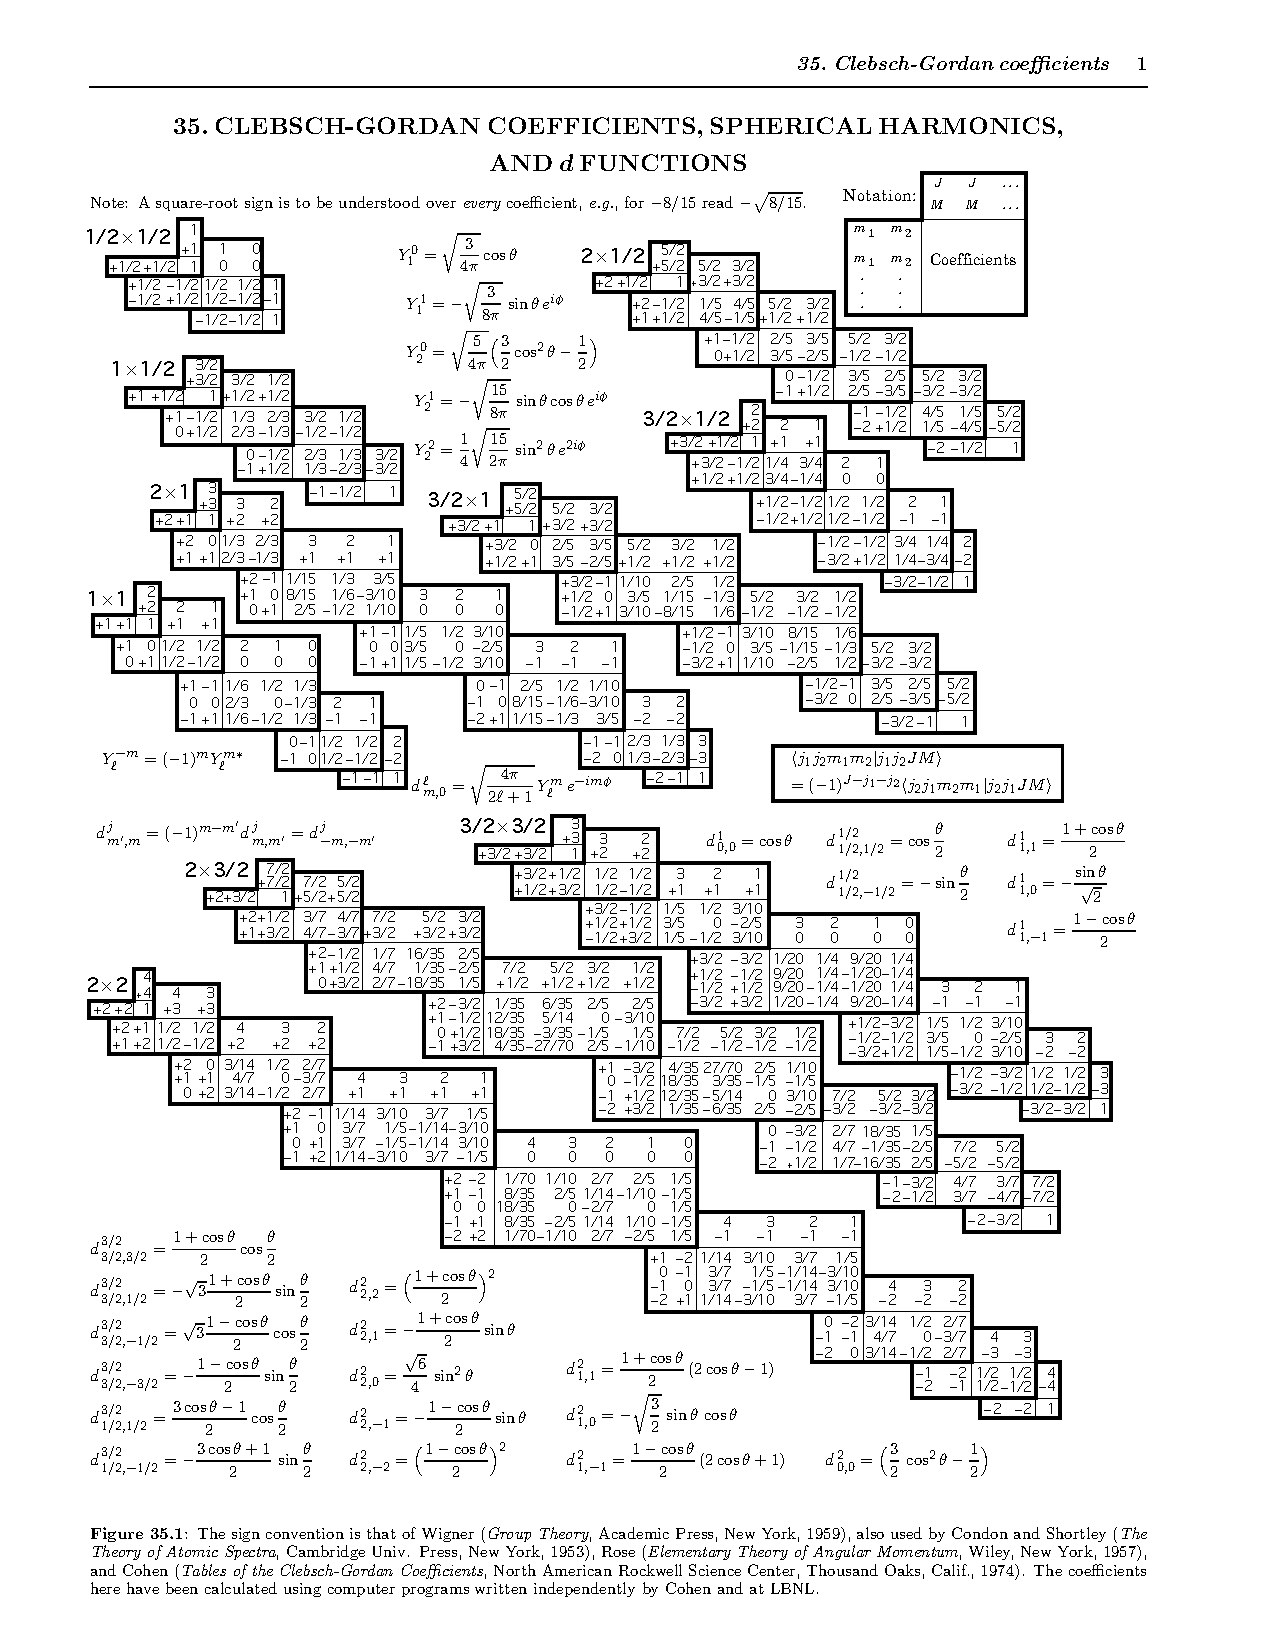
\includepdf[pages=1]{Coeficientes Clebsch-Gordan.pdf}
\end{document}
